\documentclass[./main.tex]{subfiles} 
\begin{document}

\subsection{Adaptive Step Sizes}

\subsubsection{Implemented GASS Algorithms}
Gradient Adaptive Step-Size Algorithms are designed to change the step size as the algorithm progresses. They all rely on optimising gradient descent so as to iterate quickly down a steep gradient, and then remain very stable when in steady state At the start, a large step size is needed in order for the algorithm to converge quickly, but during steady state a small step size helps to reduce the steady state error (as we have observed in previous parts of this coursework).

The LMS algorithm remains the same in structure, but $\mu$ now becomes $\mu(n)$, thus becoming $  \mathbf{w}(n+1) = \mathbf{w}(n) + \mu(n) e(n) \mathbf{x}(n) $. The algorithm to update the weight is defined as $ \mu(n+1) = \mu(n) + \rho e(n) \mathbf{x}^T(n) \boldsymbol{\psi}(n)$. $ \boldsymbol{\psi}(n) $ is defined by three different GASS algorithms, listed below:

\begin{description}
	\item[Matthews \& Xie] $  \boldsymbol{\psi}(n) = e(n-1) \mathbf{x}(n-1) $
	\item[Ang \& Farhang] $  \boldsymbol{\psi}(n) = \alpha  \boldsymbol{\psi}(n - 1) +  e(n-1) \mathbf{x}(n-1) $
	\item[Benveniste] $ \boldsymbol{\psi} = [ \mathbf{I} - \mu(n-1) \mathbf{x}(n-1) \mathbf{x}^T(n-1)  ] \boldsymbol{\psi}(n - 1) + e(n-1) \mathbf{x}(n-1) $
\end{description}

Figure \ref{fig:3_2_a_alpha} shows the Ang \& Farhang method with different values of $\alpha$. If $ \alpha $ is set too high, there runs a risk of the system becoming unstale. We can see this when $\alpha = 0.9$.

Figure \ref{fig:3_2_a} shows the three different variants. The winner appears to be the Benveniste algorithm, which overtakes everyt other algorithm to come in to steady state first. This is followed closely by the Ang \& Farhang filter, and lastly Matthews \& Xie. Overall, they clearly able to converge faster than the standard LMS algorithm, whilst at the same time remaining with a low steady state error.

\begin{figure}[h]
	\centering 
	\resizebox{\textwidth}{!}{% This file was created by matlab2tikz v0.4.7 (commit d4c8764c3916fd1d124533205db34e93e01e5518) running on MATLAB 8.3.
% Copyright (c) 2008--2014, Nico Schlömer <nico.schloemer@gmail.com>
% All rights reserved.
% Minimal pgfplots version: 1.3
% 
% The latest updates can be retrieved from
%   http://www.mathworks.com/matlabcentral/fileexchange/22022-matlab2tikz
% where you can also make suggestions and rate matlab2tikz.
% 
%
% defining custom colors
\definecolor{mycolor1}{rgb}{0.00000,0.00000,0.17241}%
\definecolor{mycolor2}{rgb}{1.00000,0.10345,0.72414}%
\definecolor{mycolor3}{rgb}{1.00000,0.82759,0.00000}%
%
\begin{tikzpicture}

\begin{axis}[%
width=8in,
height=1.5in,
scale only axis,
xmin=1,
xmax=1000,
xlabel={Iteration},
xmajorgrids,
ymin=-1,
ymax=2,
ylabel={Weight Error ($\widehat{w}(n)$)},
ymajorgrids,
title={Ang \& Farhang method for varying $\alpha$ values, and LMS reference},
axis x line*=bottom,
axis y line*=left,
legend style={draw=black,fill=white,legend cell align=left}
]
\addplot [color=blue,solid]
  table[row sep=crcr]{1	0.9\\
2	0.9\\
3	0.9\\
4	0.898063468392716\\
5	0.889510365783805\\
6	0.884624014014892\\
7	0.872939024585259\\
8	0.863750892705501\\
9	0.856884659817126\\
10	0.854509442359012\\
11	0.849349890403534\\
12	0.84369381816522\\
13	0.836821964311709\\
14	0.834936239063943\\
15	0.830877846353067\\
16	0.829046823591762\\
17	0.822908554869576\\
18	0.812240026530122\\
19	0.798932002800025\\
20	0.796655713975507\\
21	0.793852336357437\\
22	0.786788979336184\\
23	0.783319399370575\\
24	0.780264308837222\\
25	0.777741374996702\\
26	0.774067878734302\\
27	0.769033143782356\\
28	0.765130805534964\\
29	0.757979307606796\\
30	0.755418204337953\\
31	0.752557312619419\\
32	0.750261994607432\\
33	0.746900942456865\\
34	0.740567895200356\\
35	0.737726852744418\\
36	0.736502367432628\\
37	0.732877471880847\\
38	0.724964536470961\\
39	0.721789128431343\\
40	0.720961480618713\\
41	0.718519078081759\\
42	0.715346392263514\\
43	0.712553277232312\\
44	0.711032713248978\\
45	0.704802663966331\\
46	0.703467716161464\\
47	0.701739923173923\\
48	0.698360589751634\\
49	0.691765176300399\\
50	0.68669489657583\\
51	0.684704431156961\\
52	0.683210081819328\\
53	0.678074105697867\\
54	0.672936280715157\\
55	0.667174302915542\\
56	0.65680645186523\\
57	0.653883803469256\\
58	0.650050006356659\\
59	0.647944439066232\\
60	0.6451331460614\\
61	0.643703480868166\\
62	0.640220105206158\\
63	0.636095488084079\\
64	0.632595401200337\\
65	0.63026581634817\\
66	0.628265050862176\\
67	0.624893153245689\\
68	0.618891566323761\\
69	0.612366856676795\\
70	0.612014756473539\\
71	0.608540714928466\\
72	0.606209117155105\\
73	0.600273557510342\\
74	0.594867752491725\\
75	0.593894464270728\\
76	0.591243942494446\\
77	0.589141443012189\\
78	0.587481838433709\\
79	0.584603971334838\\
80	0.580456432010172\\
81	0.579183344942319\\
82	0.57737817095233\\
83	0.57504736005463\\
84	0.570388075132772\\
85	0.564577748095757\\
86	0.558673420961386\\
87	0.555893660245998\\
88	0.551946551726602\\
89	0.547460692201647\\
90	0.545089544956598\\
91	0.542292389047789\\
92	0.539271379358745\\
93	0.537901508469391\\
94	0.534056716568729\\
95	0.532095821999424\\
96	0.529471200209997\\
97	0.526762140421016\\
98	0.521787828816175\\
99	0.517229310433593\\
100	0.513877531099947\\
101	0.512713883696568\\
102	0.508704920048779\\
103	0.507345953957028\\
104	0.504351185647916\\
105	0.501369705339306\\
106	0.496764732659361\\
107	0.494503043367232\\
108	0.492653857416263\\
109	0.488587207289299\\
110	0.482771285629106\\
111	0.479418816691183\\
112	0.476933443555698\\
113	0.473269105315236\\
114	0.467939901844577\\
115	0.465066159522414\\
116	0.462721945123255\\
117	0.458954719543276\\
118	0.456164011777971\\
119	0.452959701394648\\
120	0.449058131108952\\
121	0.446961641360704\\
122	0.445534230837925\\
123	0.443386619366317\\
124	0.441370699230678\\
125	0.439393949613508\\
126	0.435956683085206\\
127	0.434670487256592\\
128	0.433199572371431\\
129	0.428920612601756\\
130	0.427856855420996\\
131	0.426417520889931\\
132	0.42311732469951\\
133	0.421524498717014\\
134	0.41881462877076\\
135	0.416293748690601\\
136	0.415112401129399\\
137	0.41401722663809\\
138	0.412389433651668\\
139	0.410064611913287\\
140	0.407375932777808\\
141	0.404787507131864\\
142	0.402258723519272\\
143	0.39952270487811\\
144	0.39593617489506\\
145	0.391383246282232\\
146	0.388477454009048\\
147	0.386857442317713\\
148	0.383946954180323\\
149	0.381329172782539\\
150	0.377841188888615\\
151	0.375676109294928\\
152	0.373102533574536\\
153	0.369020397470551\\
154	0.368806303295876\\
155	0.366412355061939\\
156	0.364795536734818\\
157	0.362703215942528\\
158	0.357055647826827\\
159	0.356154436926353\\
160	0.354422999832303\\
161	0.352812027387414\\
162	0.349769533475324\\
163	0.347480383972933\\
164	0.346233505782209\\
165	0.345242895558272\\
166	0.343838075575617\\
167	0.339485366000638\\
168	0.335559123154563\\
169	0.331846533404787\\
170	0.329324117274174\\
171	0.325808452214275\\
172	0.324746026730445\\
173	0.322023147335607\\
174	0.320228295505891\\
175	0.319002782506494\\
176	0.31764998505903\\
177	0.314864312641482\\
178	0.31347311414704\\
179	0.310446411928752\\
180	0.310188717205737\\
181	0.307311749102126\\
182	0.306938974238001\\
183	0.304592793889421\\
184	0.301884898310672\\
185	0.299556418862356\\
186	0.297481213207481\\
187	0.295406179764299\\
188	0.293513747284829\\
189	0.292969789343225\\
190	0.290342228787596\\
191	0.288608725154421\\
192	0.285980809310556\\
193	0.282107862696112\\
194	0.279569763836268\\
195	0.278630717161968\\
196	0.275872573854475\\
197	0.274359111425492\\
198	0.273082489786246\\
199	0.270508964247593\\
200	0.269468525920387\\
201	0.268546759410345\\
202	0.266413029467622\\
203	0.264737982649135\\
204	0.262191011284938\\
205	0.259430735228204\\
206	0.25634665495106\\
207	0.254172809968588\\
208	0.253111427768983\\
209	0.25224760289739\\
210	0.251383165299208\\
211	0.249173522617797\\
212	0.247456570434453\\
213	0.244224877016274\\
214	0.241690446411711\\
215	0.240984187302277\\
216	0.239480284915596\\
217	0.238705381768088\\
218	0.237042323315926\\
219	0.236851038603678\\
220	0.235127240843081\\
221	0.234771799499662\\
222	0.23413066515187\\
223	0.232696218823275\\
224	0.231430156834283\\
225	0.230611533859484\\
226	0.229141858609003\\
227	0.226212162813138\\
228	0.225960459451843\\
229	0.224939830358737\\
230	0.222662769382954\\
231	0.220872580073595\\
232	0.219729463244829\\
233	0.217767524179935\\
234	0.215536877899623\\
235	0.212167076013699\\
236	0.21100759008824\\
237	0.209149493351456\\
238	0.207891643145014\\
239	0.20682679348894\\
240	0.205638995228459\\
241	0.204338965753053\\
242	0.203075005354655\\
243	0.202523329589431\\
244	0.20092817748786\\
245	0.19932185421537\\
246	0.197718110551496\\
247	0.19685324518034\\
248	0.195461719395536\\
249	0.193608445709636\\
250	0.192749962283207\\
251	0.191358629324326\\
252	0.190571433654329\\
253	0.188674968518346\\
254	0.187705112980578\\
255	0.187065030541377\\
256	0.186389690070259\\
257	0.184607053290465\\
258	0.18255904141026\\
259	0.181641318411197\\
260	0.179848308946298\\
261	0.17900065190892\\
262	0.176495522496022\\
263	0.175542054589693\\
264	0.173738425431657\\
265	0.172521874283517\\
266	0.171193266172479\\
267	0.170794499721545\\
268	0.169221223612417\\
269	0.167109420246054\\
270	0.164672323554695\\
271	0.163719959043568\\
272	0.162823966895045\\
273	0.161564339697358\\
274	0.16066192322757\\
275	0.159900932842582\\
276	0.157895534247643\\
277	0.156844557227764\\
278	0.155485653778517\\
279	0.15477536216664\\
280	0.152838684622595\\
281	0.152258496151472\\
282	0.149904462293112\\
283	0.149142764417432\\
284	0.147646016550849\\
285	0.146093626357734\\
286	0.145153813031855\\
287	0.143599590340034\\
288	0.141324108284106\\
289	0.140624844746672\\
290	0.13927650267002\\
291	0.138358926274837\\
292	0.137545369636866\\
293	0.136559928828642\\
294	0.135039718528965\\
295	0.133557638550399\\
296	0.132113811024686\\
297	0.130954799467809\\
298	0.130000808534372\\
299	0.128488831472524\\
300	0.1275045973853\\
301	0.12620190930544\\
302	0.125313614568886\\
303	0.124393761532116\\
304	0.122957710232534\\
305	0.121889849519885\\
306	0.120049301583009\\
307	0.117754420457463\\
308	0.117099908512702\\
309	0.115038045046618\\
310	0.113991493972262\\
311	0.11196141496527\\
312	0.110658549101239\\
313	0.108632266286138\\
314	0.107167433184033\\
315	0.106219216013914\\
316	0.105658687848085\\
317	0.104122983373128\\
318	0.103589108581532\\
319	0.102169236368133\\
320	0.101868866606053\\
321	0.101171232485705\\
322	0.100157243133516\\
323	0.0997011496099163\\
324	0.0988222183646299\\
325	0.0978988525051838\\
326	0.0966620004942073\\
327	0.096008642694889\\
328	0.0943998881428411\\
329	0.0937001078732861\\
330	0.0924747601840155\\
331	0.0917551445797579\\
332	0.0916130281659909\\
333	0.0909763520008458\\
334	0.0897550694822554\\
335	0.0886651867715369\\
336	0.0879448434373676\\
337	0.0863118014204816\\
338	0.0853071435892527\\
339	0.0849980216077837\\
340	0.0845328707732511\\
341	0.0837945817188848\\
342	0.0827499583988839\\
343	0.0824121494169546\\
344	0.0808186668580507\\
345	0.0792266391006029\\
346	0.0777008055150086\\
347	0.0764715152970864\\
348	0.0758367194284094\\
349	0.0747783320629314\\
350	0.0741244637362221\\
351	0.0724335960014351\\
352	0.071538828909814\\
353	0.0706412543967563\\
354	0.0688066310539588\\
355	0.0685620807099037\\
356	0.0678709600124078\\
357	0.0670481729356699\\
358	0.0662687315698872\\
359	0.0655050814150305\\
360	0.0644400707270647\\
361	0.0637265895064729\\
362	0.0625900787527879\\
363	0.0622012333984217\\
364	0.061656269844468\\
365	0.0601701747194975\\
366	0.0591853431691455\\
367	0.0578737710198983\\
368	0.0574300868679306\\
369	0.0562324317301995\\
370	0.0548581025528579\\
371	0.0538122226491847\\
372	0.0532408082727279\\
373	0.0523284339651081\\
374	0.0513751182914556\\
375	0.0509632909702722\\
376	0.0497081339364812\\
377	0.0495409373566184\\
378	0.0490419975052863\\
379	0.0480031098459549\\
380	0.0471958448351545\\
381	0.0463510070252368\\
382	0.0453770660310466\\
383	0.0440658943761072\\
384	0.0433423830424937\\
385	0.0432103075811349\\
386	0.0421451493259424\\
387	0.0413798261897945\\
388	0.0411275744166739\\
389	0.0407203644391333\\
390	0.0399547963361159\\
391	0.0392377004900201\\
392	0.0389342061787845\\
393	0.0383923269765963\\
394	0.0381942680420357\\
395	0.0377880615292835\\
396	0.0376472950122245\\
397	0.0374654692816326\\
398	0.0365642806474663\\
399	0.036392274235897\\
400	0.0360403660451123\\
401	0.035060855433118\\
402	0.034783211332205\\
403	0.0339747668369433\\
404	0.0329162757537889\\
405	0.0325370005968665\\
406	0.0319730227786513\\
407	0.0317232366339971\\
408	0.0308387161617475\\
409	0.0306182716475801\\
410	0.0292350836629002\\
411	0.0290184830578326\\
412	0.0276267242778678\\
413	0.0265304611662822\\
414	0.0253801177343913\\
415	0.0248547668740413\\
416	0.0245184593935667\\
417	0.0240643344923124\\
418	0.0232163372685855\\
419	0.0230061959499061\\
420	0.0225957469678761\\
421	0.0222143526540898\\
422	0.0216490416105709\\
423	0.0213277004242757\\
424	0.0210821184845381\\
425	0.0203443784436893\\
426	0.0201742460605662\\
427	0.0192765560462814\\
428	0.0188843296338572\\
429	0.0178236772262418\\
430	0.0175083685680839\\
431	0.0167334804420168\\
432	0.0162018920930892\\
433	0.0153125706738763\\
434	0.0143654402786785\\
435	0.0133749625607067\\
436	0.0130290201406407\\
437	0.0125209980889931\\
438	0.0118356307483156\\
439	0.0109594438344012\\
440	0.010508670263456\\
441	0.0101051233557378\\
442	0.00935899466139589\\
443	0.00857297031600623\\
444	0.00841406558985158\\
445	0.00732647244299833\\
446	0.00702725233583357\\
447	0.0067946062325247\\
448	0.00657234282810837\\
449	0.00562301410479193\\
450	0.00490299256581894\\
451	0.00464326958659178\\
452	0.00421335455555105\\
453	0.00369238953347595\\
454	0.00321529201171333\\
455	0.00291159745943659\\
456	0.00217410779700933\\
457	0.00180688480601643\\
458	0.00117640098462213\\
459	0.000727326914557347\\
460	0.000421240927260591\\
461	-0.000149001135964277\\
462	-0.00052475937400509\\
463	-0.00097474277186127\\
464	-0.00134608135142589\\
465	-0.00194000856468435\\
466	-0.00257122250184183\\
467	-0.00320287047153178\\
468	-0.00370186671710038\\
469	-0.00421440461263045\\
470	-0.00461134188639545\\
471	-0.00489956021812576\\
472	-0.00514189429919598\\
473	-0.00559761051580221\\
474	-0.00608230366442564\\
475	-0.00641694215894151\\
476	-0.00661031877622054\\
477	-0.0069506070701516\\
478	-0.00733349755856361\\
479	-0.00783833587221205\\
480	-0.00854397085131531\\
481	-0.00863261698849127\\
482	-0.00915163669786978\\
483	-0.00965206061572021\\
484	-0.0100213662833474\\
485	-0.010379278058067\\
486	-0.0112794661265019\\
487	-0.0115326971764803\\
488	-0.0117142036987173\\
489	-0.0119585556779397\\
490	-0.0124832033865599\\
491	-0.0126138341779247\\
492	-0.0138038000747729\\
493	-0.0146711603761535\\
494	-0.0155181765967762\\
495	-0.0157545382736243\\
496	-0.0159570515626237\\
497	-0.0171447553517249\\
498	-0.0174458746622509\\
499	-0.0179026018057381\\
500	-0.0182757358393442\\
501	-0.0187499849869465\\
502	-0.0191133882626738\\
503	-0.0197651196195322\\
504	-0.0202688103585315\\
505	-0.0205466519696351\\
506	-0.0208257642712766\\
507	-0.0209152179815276\\
508	-0.0210473220772993\\
509	-0.021529122369231\\
510	-0.0219628134947308\\
511	-0.022297713398412\\
512	-0.0229770078604117\\
513	-0.0232817576629875\\
514	-0.0237627974233392\\
515	-0.0241960908698392\\
516	-0.0243686476883553\\
517	-0.0248899719080125\\
518	-0.0253719099346466\\
519	-0.0260890670752013\\
520	-0.0260956882305556\\
521	-0.0260735587008758\\
522	-0.0263303926402779\\
523	-0.0266300249097148\\
524	-0.0273008987205818\\
525	-0.0276048209719221\\
526	-0.0278845960151576\\
527	-0.0282725065950803\\
528	-0.0285510161016923\\
529	-0.0289045166456635\\
530	-0.0294007060734554\\
531	-0.0297143900858208\\
532	-0.0301193421262146\\
533	-0.0308655773312569\\
534	-0.0312842037919271\\
535	-0.031626312411927\\
536	-0.031725662765832\\
537	-0.0318510972881974\\
538	-0.0322244422237704\\
539	-0.0323912964787257\\
540	-0.0329497968259147\\
541	-0.0330351462289016\\
542	-0.0332330432498645\\
543	-0.0335205162550254\\
544	-0.0338986075862143\\
545	-0.0343504843641744\\
546	-0.034763165603889\\
547	-0.0348852704147949\\
548	-0.0352349041263181\\
549	-0.0360175947626892\\
550	-0.0364188463790471\\
551	-0.0367376099763348\\
552	-0.036841331238384\\
553	-0.0372175864965835\\
554	-0.0375794649033375\\
555	-0.0381270448210962\\
556	-0.0383603701857124\\
557	-0.0389704109320937\\
558	-0.0392008989614107\\
559	-0.0394021116710848\\
560	-0.0395080208217858\\
561	-0.0396764160422238\\
562	-0.0400999921881838\\
563	-0.0407797426152926\\
564	-0.0411574337568209\\
565	-0.0411484539494831\\
566	-0.0415253017305497\\
567	-0.0417618613589376\\
568	-0.0422467029248567\\
569	-0.0425616254920947\\
570	-0.0429269004613381\\
571	-0.0432919711172751\\
572	-0.0436643517023366\\
573	-0.04413815118662\\
574	-0.0445514783769649\\
575	-0.0448835083195082\\
576	-0.0450365387518028\\
577	-0.0451772103148966\\
578	-0.0453462911378245\\
579	-0.0455602807752816\\
580	-0.0456371398997054\\
581	-0.046095967638046\\
582	-0.0461998212231979\\
583	-0.0466334845158493\\
584	-0.0471660956026537\\
585	-0.0471938500276762\\
586	-0.0475448095710795\\
587	-0.048133642706243\\
588	-0.0482868798911497\\
589	-0.0484113773418434\\
590	-0.0486115921818852\\
591	-0.0491005817558438\\
592	-0.0493806011434971\\
593	-0.0497197391054968\\
594	-0.0498565010631301\\
595	-0.0500473104500969\\
596	-0.050068364004086\\
597	-0.0505037728170297\\
598	-0.0504980295637045\\
599	-0.0506015993402179\\
600	-0.0506506694768779\\
601	-0.0510619975321628\\
602	-0.0516477405618913\\
603	-0.0518572710204257\\
604	-0.0521759589020435\\
605	-0.0523545134379102\\
606	-0.0526153312700728\\
607	-0.0527429459273675\\
608	-0.0528698009460766\\
609	-0.0531971447930519\\
610	-0.053552971096974\\
611	-0.053976106173217\\
612	-0.0541837324866667\\
613	-0.0543564447147334\\
614	-0.0544403057432422\\
615	-0.0548367918637405\\
616	-0.0551051981498062\\
617	-0.0552011038364423\\
618	-0.0554527081095963\\
619	-0.0557609085501001\\
620	-0.0558509423411984\\
621	-0.0562258567788243\\
622	-0.0563321096110879\\
623	-0.0564844640681433\\
624	-0.056766247653311\\
625	-0.0572826286642577\\
626	-0.0573514885389107\\
627	-0.0575904046958774\\
628	-0.0576156118430828\\
629	-0.0581165081591031\\
630	-0.0582242039347518\\
631	-0.0583176466476238\\
632	-0.0585779992536956\\
633	-0.0586819055392309\\
634	-0.058808187303925\\
635	-0.058952264688716\\
636	-0.0590147735127097\\
637	-0.0591649931988021\\
638	-0.0593159018284648\\
639	-0.059565149688526\\
640	-0.0599371880262095\\
641	-0.0601560057358693\\
642	-0.0605323489258337\\
643	-0.060748679663854\\
644	-0.0609340556830764\\
645	-0.0610826647099687\\
646	-0.0613508636490715\\
647	-0.0615824535160815\\
648	-0.0618533318482092\\
649	-0.0619915472363864\\
650	-0.0621413747388988\\
651	-0.0622637494536095\\
652	-0.0623621181022024\\
653	-0.0626032482436917\\
654	-0.0627023037116625\\
655	-0.0629773793824707\\
656	-0.0632046804431166\\
657	-0.0633740760618448\\
658	-0.0635469024488386\\
659	-0.0636669884259763\\
660	-0.0638192242144981\\
661	-0.0640035316364722\\
662	-0.0641238822925915\\
663	-0.0642006352209989\\
664	-0.0644100154750843\\
665	-0.0648664248066698\\
666	-0.0651925153843234\\
667	-0.06544336075751\\
668	-0.0655881682634811\\
669	-0.0657033282752909\\
670	-0.065878990208149\\
671	-0.0662461860727814\\
672	-0.0663996198568269\\
673	-0.0666320393670256\\
674	-0.0669604213001962\\
675	-0.0670704533389542\\
676	-0.0672934811005069\\
677	-0.0674287427531304\\
678	-0.0677310420332812\\
679	-0.0678076822918167\\
680	-0.0680429046183849\\
681	-0.068294434701613\\
682	-0.0686035045711716\\
683	-0.0687063951159865\\
684	-0.0688044104370054\\
685	-0.0689514476956\\
686	-0.0690146119507119\\
687	-0.0691103217501847\\
688	-0.0693219135696649\\
689	-0.069449418404247\\
690	-0.0696830036319577\\
691	-0.0698568059671432\\
692	-0.0699608250465846\\
693	-0.0701375658840966\\
694	-0.0701450841860281\\
695	-0.0702582549709481\\
696	-0.0703215628127578\\
697	-0.0705003374023002\\
698	-0.0705745678166151\\
699	-0.0707247378353374\\
700	-0.0708731609183705\\
701	-0.0710149530725285\\
702	-0.0713190765267743\\
703	-0.0713704979022562\\
704	-0.0715095183302107\\
705	-0.0716233430960306\\
706	-0.0718596768289229\\
707	-0.0719736520606814\\
708	-0.0721647946708364\\
709	-0.0724527958304314\\
710	-0.0725723455706692\\
711	-0.0727582525266648\\
712	-0.0728610282505912\\
713	-0.0729015872073174\\
714	-0.0729799660900721\\
715	-0.07318322094938\\
716	-0.0732209263666798\\
717	-0.0732850540122889\\
718	-0.0734892344829285\\
719	-0.0737560330774147\\
720	-0.0739448567598\\
721	-0.074067957774311\\
722	-0.0741074965974012\\
723	-0.0741760195042422\\
724	-0.0742895320748467\\
725	-0.0743518131542175\\
726	-0.0744801808529253\\
727	-0.0746826706362235\\
728	-0.0747177854270485\\
729	-0.0750289038456927\\
730	-0.0751838507057988\\
731	-0.0752542123141333\\
732	-0.0753430763669153\\
733	-0.0753609614567203\\
734	-0.0754398558214395\\
735	-0.0756394894096528\\
736	-0.0757570014548042\\
737	-0.0758596969803722\\
738	-0.0759450115664176\\
739	-0.0759778921571351\\
740	-0.0760576559588388\\
741	-0.0762058225457843\\
742	-0.0762718770526307\\
743	-0.0763287823673913\\
744	-0.0765646410452129\\
745	-0.0766864868628883\\
746	-0.0768053875120059\\
747	-0.076907361979707\\
748	-0.0770899038794611\\
749	-0.0771306817612721\\
750	-0.077237319226621\\
751	-0.0773811149046733\\
752	-0.0774572980539563\\
753	-0.0775714937753529\\
754	-0.0776682403403989\\
755	-0.0777058727137511\\
756	-0.0777329001168324\\
757	-0.0778265755035985\\
758	-0.0779537163161059\\
759	-0.0780786830035966\\
760	-0.0782727194026511\\
761	-0.0784387546427361\\
762	-0.0785118596271511\\
763	-0.07854745486388\\
764	-0.0787011187473752\\
765	-0.0787313268108824\\
766	-0.0788155408584934\\
767	-0.0789388225951423\\
768	-0.0789965442667153\\
769	-0.0790597943002778\\
770	-0.0791571280203379\\
771	-0.0791887021390462\\
772	-0.0794682753607009\\
773	-0.0796080137066647\\
774	-0.0797474869432954\\
775	-0.0798967783424495\\
776	-0.0800011298236404\\
777	-0.0800503359606118\\
778	-0.0801100708921837\\
779	-0.0802428190411163\\
780	-0.0802837346927274\\
781	-0.0803868918324138\\
782	-0.0804990635880312\\
783	-0.0807080426508507\\
784	-0.0808218582352257\\
785	-0.0808561911625986\\
786	-0.0810135245430569\\
787	-0.0810872182592808\\
788	-0.0812017326554125\\
789	-0.0812339776125498\\
790	-0.0812888512472995\\
791	-0.0813406741264645\\
792	-0.0814431640359506\\
793	-0.0814720624565322\\
794	-0.0815690089072978\\
795	-0.0817542353307809\\
796	-0.0818817520669153\\
797	-0.0819708590539855\\
798	-0.0820660750151599\\
799	-0.0821864000565643\\
800	-0.0822558164595003\\
801	-0.0823417834875387\\
802	-0.0824505726954108\\
803	-0.0824987424767812\\
804	-0.0825708719527757\\
805	-0.0826407324443791\\
806	-0.0827056942233003\\
807	-0.0828434186975974\\
808	-0.0829581369820758\\
809	-0.0831278247211725\\
810	-0.0832405455240968\\
811	-0.0832671791658285\\
812	-0.0834021828287076\\
813	-0.0834790012104261\\
814	-0.0835301003506176\\
815	-0.0836267210447843\\
816	-0.0836921712006472\\
817	-0.0837740294481915\\
818	-0.0838417079876077\\
819	-0.0839722780219381\\
820	-0.0840639363714801\\
821	-0.0840890215059827\\
822	-0.0842033661229574\\
823	-0.0842355871258339\\
824	-0.0842925610525856\\
825	-0.084413010840288\\
826	-0.0844653448149947\\
827	-0.0845489328757815\\
828	-0.0846070500755838\\
829	-0.0846723019645369\\
830	-0.0847944262402954\\
831	-0.0849825029649132\\
832	-0.0851567636214146\\
833	-0.0851856491212374\\
834	-0.0852647812623767\\
835	-0.0853467326100983\\
836	-0.0854100910098473\\
837	-0.0854907743431976\\
838	-0.0855758277052269\\
839	-0.0856128065945519\\
840	-0.0857113747465892\\
841	-0.0858001860556911\\
842	-0.0858459886476947\\
843	-0.0859010121719291\\
844	-0.0859670244137882\\
845	-0.086006424408447\\
846	-0.0860422110824889\\
847	-0.0861104197466541\\
848	-0.0861887171538137\\
849	-0.0862782300926339\\
850	-0.0863803141800626\\
851	-0.0864167402114908\\
852	-0.0864749167621053\\
853	-0.0865035454664177\\
854	-0.0865600842646623\\
855	-0.08667571294062\\
856	-0.0867434846093138\\
857	-0.0868865479765683\\
858	-0.0869677961738713\\
859	-0.0870289803420722\\
860	-0.0871024939139955\\
861	-0.0871797595489374\\
862	-0.0872091782821395\\
863	-0.087345073492938\\
864	-0.0874260027756726\\
865	-0.0875429824968256\\
866	-0.0875729521858133\\
867	-0.0876041079222121\\
868	-0.0876577383287419\\
869	-0.087684808939583\\
870	-0.0877462206096645\\
871	-0.0878252236371759\\
872	-0.0878961498616171\\
873	-0.0879424260651852\\
874	-0.0880729673063915\\
875	-0.0881292644738571\\
876	-0.0882375677073776\\
877	-0.088319489966272\\
878	-0.0883819273350649\\
879	-0.0884717398397018\\
880	-0.088577895676447\\
881	-0.0885905861898283\\
882	-0.0886632151544923\\
883	-0.0886684846408163\\
884	-0.0886816354069803\\
885	-0.0887071508883902\\
886	-0.0888113985260542\\
887	-0.088846461360008\\
888	-0.0888768366638885\\
889	-0.0890092168551423\\
890	-0.0890183426676249\\
891	-0.0891389477039418\\
892	-0.0891537172219034\\
893	-0.089187470682339\\
894	-0.0892335132435393\\
895	-0.0892974814018878\\
896	-0.0893413086284077\\
897	-0.0893924955320452\\
898	-0.0893982615353938\\
899	-0.0894922293764352\\
900	-0.0895372125914049\\
901	-0.0895463641616324\\
902	-0.0895750989674793\\
903	-0.0895976760021897\\
904	-0.0896985461444496\\
905	-0.0897470011130561\\
906	-0.0897727098649739\\
907	-0.0898859599850456\\
908	-0.089927484082194\\
909	-0.0899549130137315\\
910	-0.0899713791725217\\
911	-0.089993365480317\\
912	-0.0900577681393898\\
913	-0.0901036030416495\\
914	-0.0901595617554889\\
915	-0.0902386490536031\\
916	-0.0902635564427717\\
917	-0.0903220107710625\\
918	-0.0903215561497438\\
919	-0.0903553223295682\\
920	-0.0904446942312337\\
921	-0.0905341682117823\\
922	-0.0906010027631987\\
923	-0.0906550199182007\\
924	-0.0907134178003083\\
925	-0.0907578517828211\\
926	-0.0907906827558129\\
927	-0.090821511168139\\
928	-0.0908573218197644\\
929	-0.0908751118165793\\
930	-0.0909399853949349\\
931	-0.0909706111901384\\
932	-0.0909910607173018\\
933	-0.0910185402122119\\
934	-0.0910572676342347\\
935	-0.0911332950185672\\
936	-0.0911533443007558\\
937	-0.0911861025643809\\
938	-0.0912293429086658\\
939	-0.0912630406311942\\
940	-0.0913050839894562\\
941	-0.0913392540442591\\
942	-0.0913684821073941\\
943	-0.0913937355137188\\
944	-0.0914326542861772\\
945	-0.0914882220666324\\
946	-0.0915299583904827\\
947	-0.0916138985124506\\
948	-0.0916561049365656\\
949	-0.0916938404048292\\
950	-0.0917263556255241\\
951	-0.0917931727342972\\
952	-0.0918724848810745\\
953	-0.0919709953795891\\
954	-0.0919687781553031\\
955	-0.0919864960512535\\
956	-0.0920279647505102\\
957	-0.09205494538091\\
958	-0.0921176674425661\\
959	-0.0921542367797359\\
960	-0.092202633463853\\
961	-0.0922448287065446\\
962	-0.0923019050802446\\
963	-0.0923221251563854\\
964	-0.092419873713839\\
965	-0.0924246702280553\\
966	-0.0924425538738652\\
967	-0.092475977133347\\
968	-0.0925128408094499\\
969	-0.0925285895008177\\
970	-0.0925691248351151\\
971	-0.0925941183904717\\
972	-0.092667919083902\\
973	-0.0927181045208361\\
974	-0.0927290801339541\\
975	-0.0927463592861144\\
976	-0.0928152828063519\\
977	-0.0928718265335318\\
978	-0.0928993111165644\\
979	-0.0929170113204076\\
980	-0.0929313443848022\\
981	-0.0929621950692457\\
982	-0.0929746974401501\\
983	-0.0930458308116877\\
984	-0.0930743212558933\\
985	-0.0931066380415057\\
986	-0.0931247818287205\\
987	-0.0932066033281408\\
988	-0.0932407959944174\\
989	-0.0932724197139991\\
990	-0.0933221560794425\\
991	-0.0933448344614236\\
992	-0.0933988444305821\\
993	-0.0934501134537223\\
994	-0.0935053778647486\\
995	-0.093595416947266\\
996	-0.0936223601702979\\
997	-0.0936607291533761\\
998	-0.093685289861936\\
999	-0.0936973547664498\\
1000	-0.0937127133211531\\
1001	-0.0937562371364216\\
};
\addlegendentry{$\text{LMS: }\mu\text{ =0.010}$};

\addplot [color=red,solid]
  table[row sep=crcr]{1	0.9\\
2	0.9\\
3	0.9\\
4	0.880634683927159\\
5	0.796878906841435\\
6	0.757083551925932\\
7	0.67216035342206\\
8	0.601168637545311\\
9	0.557053467058689\\
10	0.541954706171976\\
11	0.50501814018424\\
12	0.467238854775631\\
13	0.428820589490061\\
14	0.416075622925561\\
15	0.397950310416375\\
16	0.389545801955795\\
17	0.354442988330682\\
18	0.290893414553614\\
19	0.213629284888421\\
20	0.203078594749372\\
21	0.191048729176928\\
22	0.171618058826812\\
23	0.160620093843716\\
24	0.15108183589722\\
25	0.14363467499103\\
26	0.13440048906888\\
27	0.121091323081478\\
28	0.11342581906203\\
29	0.0970932862111228\\
30	0.0923541638311273\\
31	0.084811253842206\\
32	0.0795524777798458\\
33	0.0734346308303847\\
34	0.0624879970281924\\
35	0.0589027058988825\\
36	0.0570812562100066\\
37	0.0472606474097654\\
38	0.0371106151227235\\
39	0.0303602719446335\\
40	0.0295925477888312\\
41	0.0261773896240636\\
42	0.0219105811122321\\
43	0.0191668028616308\\
44	0.0177323503258962\\
45	0.00534552283454637\\
46	0.00269912951088325\\
47	-0.0016377258794541\\
48	-0.00337515130952681\\
49	-0.0130587758092924\\
50	-0.020307956315072\\
51	-0.0228784414770287\\
52	-0.0239522790263941\\
53	-0.0285967889969824\\
54	-0.0347315578159886\\
55	-0.0399053882309631\\
56	-0.0500226382836603\\
57	-0.0506311462661371\\
58	-0.0529609413653824\\
59	-0.0541704249380007\\
60	-0.056083434951687\\
61	-0.0567261825292392\\
62	-0.0581463864935384\\
63	-0.0605194337005797\\
64	-0.0615898985107438\\
65	-0.0629262769867146\\
66	-0.0644878654173363\\
67	-0.0669493025774415\\
68	-0.0702563029056946\\
69	-0.0741312060951392\\
70	-0.0740570809034544\\
71	-0.0749422410595944\\
72	-0.0757056691798935\\
73	-0.0774591442016562\\
74	-0.0794130888267871\\
75	-0.0798085108015402\\
76	-0.0805089938848464\\
77	-0.0811879140112453\\
78	-0.0816579280168487\\
79	-0.0823235774419278\\
80	-0.083706238518115\\
81	-0.0837679761770769\\
82	-0.0841534242719163\\
83	-0.0846480002584575\\
84	-0.0854418031353958\\
85	-0.0874770470940699\\
86	-0.088958339633702\\
87	-0.0895081898670156\\
88	-0.090387446896215\\
89	-0.0911797898726167\\
90	-0.0914137451742478\\
91	-0.0917533694398143\\
92	-0.0920110060218607\\
93	-0.0921632233724384\\
94	-0.0926741088541296\\
95	-0.0928874169707462\\
96	-0.0932744052695051\\
97	-0.09349453475365\\
98	-0.0938161910237474\\
99	-0.0942743245240123\\
100	-0.0945982154174719\\
101	-0.0946868726943085\\
102	-0.0949937891977567\\
103	-0.0951641534690291\\
104	-0.0955073553223229\\
105	-0.0957162085190305\\
106	-0.0960603554601837\\
107	-0.0962217201485857\\
108	-0.0963796894485469\\
109	-0.0966981140627459\\
110	-0.0971309039439686\\
111	-0.0973636046605756\\
112	-0.0974293931593069\\
113	-0.097530823637501\\
114	-0.0977014489648732\\
115	-0.0977878549977029\\
116	-0.0979142923822979\\
117	-0.0980919280877195\\
118	-0.0982085888698885\\
119	-0.0982784984899002\\
120	-0.0985015989421828\\
121	-0.0985719416232237\\
122	-0.0986119700164355\\
123	-0.0986525178916465\\
124	-0.098681901462415\\
125	-0.098729567690632\\
126	-0.0987869395822827\\
127	-0.098843430158703\\
128	-0.0988720202041745\\
129	-0.0990023742362774\\
130	-0.0990259758539608\\
131	-0.0990512645055869\\
132	-0.0991212345016175\\
133	-0.0991640035476639\\
134	-0.0991944508200852\\
135	-0.0992468991727605\\
136	-0.0992694756207589\\
137	-0.0992865817335035\\
138	-0.0993052011809309\\
139	-0.0993675117021989\\
140	-0.0993991356090996\\
141	-0.0994227366076031\\
142	-0.09944482577689\\
143	-0.0994656341940423\\
144	-0.0994977904044724\\
145	-0.0995732619506526\\
146	-0.099598669796885\\
147	-0.0996078911970212\\
148	-0.0996429753981365\\
149	-0.0996748190124295\\
150	-0.0996975584694645\\
151	-0.0997144065888731\\
152	-0.0997254889006983\\
153	-0.0997406531394267\\
154	-0.0997432377516601\\
155	-0.0997538098720738\\
156	-0.0997632482242981\\
157	-0.0997714269516595\\
158	-0.0997888426859151\\
159	-0.0997917342751545\\
160	-0.0998035315516589\\
161	-0.0998110712066997\\
162	-0.0998205256853156\\
163	-0.0998308927303668\\
164	-0.0998336436381816\\
165	-0.0998387719882649\\
166	-0.0998447698720151\\
167	-0.0998640790177736\\
168	-0.0998837534512583\\
169	-0.0998982949864269\\
170	-0.0999025271791556\\
171	-0.0999131621371422\\
172	-0.0999141045344348\\
173	-0.0999181475026507\\
174	-0.0999220142468825\\
175	-0.0999259669735065\\
176	-0.0999277783207578\\
177	-0.0999326023075211\\
178	-0.0999351372562046\\
179	-0.0999409293768202\\
180	-0.0999403080860436\\
181	-0.0999437167847723\\
182	-0.0999441303482937\\
183	-0.0999478832747235\\
184	-0.0999532969918977\\
185	-0.0999571984534313\\
186	-0.099960139784158\\
187	-0.0999623502771448\\
188	-0.0999640175608677\\
189	-0.0999645925107652\\
190	-0.0999668701176926\\
191	-0.0999683509831\\
192	-0.0999701699901203\\
193	-0.0999731732100633\\
194	-0.0999754107885433\\
195	-0.0999757702393237\\
196	-0.0999781421025053\\
197	-0.0999787681654475\\
198	-0.0999797100005769\\
199	-0.0999812131439226\\
200	-0.0999818049150966\\
201	-0.099982127410578\\
202	-0.0999828787958051\\
203	-0.0999839525572362\\
204	-0.0999847323862459\\
205	-0.0999853619511631\\
206	-0.0999870566090798\\
207	-0.0999872539192139\\
208	-0.0999880067341733\\
209	-0.0999882704448879\\
210	-0.0999883465065637\\
211	-0.0999889187925976\\
212	-0.0999898905802441\\
213	-0.0999905391521355\\
214	-0.0999912364075891\\
215	-0.0999912563212607\\
216	-0.0999921914437504\\
217	-0.099992105862159\\
218	-0.0999925162399019\\
219	-0.0999925199079882\\
220	-0.0999927450258001\\
221	-0.0999929653066622\\
222	-0.0999930433713981\\
223	-0.0999935275451909\\
224	-0.0999936150471111\\
225	-0.0999939343245273\\
226	-0.0999943802848987\\
227	-0.0999949576813703\\
228	-0.0999949128389849\\
229	-0.0999949957167992\\
230	-0.0999953689880444\\
231	-0.0999954573503368\\
232	-0.0999956382048998\\
233	-0.099995782142577\\
234	-0.0999959582920515\\
235	-0.0999962102996788\\
236	-0.0999964935405965\\
237	-0.0999967990579161\\
238	-0.0999968678780908\\
239	-0.0999969236558372\\
240	-0.0999970212154376\\
241	-0.0999971062574891\\
242	-0.0999972958923997\\
243	-0.0999973299783686\\
244	-0.0999974368990025\\
245	-0.0999976779816426\\
246	-0.099997799596277\\
247	-0.0999978281044516\\
248	-0.0999978929326291\\
249	-0.0999981242303617\\
250	-0.0999981256728245\\
251	-0.0999981738618195\\
252	-0.099998213891588\\
253	-0.0999983500844465\\
254	-0.0999983660911441\\
255	-0.0999984211748627\\
256	-0.0999984598288002\\
257	-0.0999986033255468\\
258	-0.0999988134251747\\
259	-0.0999989159732292\\
260	-0.0999990167104414\\
261	-0.0999990293041605\\
262	-0.0999990725375308\\
263	-0.0999990880952196\\
264	-0.0999991489615419\\
265	-0.0999991780380526\\
266	-0.0999991950361562\\
267	-0.0999992171202821\\
268	-0.0999992376548213\\
269	-0.0999993136497724\\
270	-0.0999993385354331\\
271	-0.0999993641168299\\
272	-0.0999993856911038\\
273	-0.0999994180224553\\
274	-0.0999994413727654\\
275	-0.0999994553893764\\
276	-0.0999994813498238\\
277	-0.0999995026026698\\
278	-0.0999995322130299\\
279	-0.0999995423151787\\
280	-0.0999995912628193\\
281	-0.0999995958514379\\
282	-0.0999996120139804\\
283	-0.0999996220042355\\
284	-0.0999996669688642\\
285	-0.0999997057521268\\
286	-0.0999997193898033\\
287	-0.0999997363352255\\
288	-0.0999997591237596\\
289	-0.0999997617742172\\
290	-0.0999997741501005\\
291	-0.0999997814947811\\
292	-0.0999997923427617\\
293	-0.0999998007561255\\
294	-0.0999998132587387\\
295	-0.099999824848398\\
296	-0.0999998415767696\\
297	-0.099999844671\\
298	-0.099999851773967\\
299	-0.0999998578951171\\
300	-0.0999998614937446\\
301	-0.0999998649143379\\
302	-0.0999998696666298\\
303	-0.0999998749119114\\
304	-0.0999998863661027\\
305	-0.0999998913951957\\
306	-0.0999999003526346\\
307	-0.0999999074808988\\
308	-0.0999999096032954\\
309	-0.0999999182618644\\
310	-0.0999999256527129\\
311	-0.099999928766114\\
312	-0.0999999363229583\\
313	-0.0999999516032222\\
314	-0.0999999551764873\\
315	-0.0999999578142123\\
316	-0.0999999590416886\\
317	-0.0999999597288731\\
318	-0.0999999607047926\\
319	-0.0999999639423867\\
320	-0.099999964627292\\
321	-0.0999999652909437\\
322	-0.0999999666299324\\
323	-0.0999999667126275\\
324	-0.0999999688283925\\
325	-0.0999999701930828\\
326	-0.0999999715673663\\
327	-0.0999999732848634\\
328	-0.0999999780527455\\
329	-0.0999999785072055\\
330	-0.0999999795933787\\
331	-0.0999999805000554\\
332	-0.0999999805451827\\
333	-0.0999999809919189\\
334	-0.0999999825199468\\
335	-0.0999999831282942\\
336	-0.099999984493747\\
337	-0.099999986000095\\
338	-0.099999986820588\\
339	-0.0999999872837334\\
340	-0.0999999877158215\\
341	-0.0999999881384502\\
342	-0.0999999890723148\\
343	-0.0999999891321804\\
344	-0.0999999902750133\\
345	-0.099999991333689\\
346	-0.099999992618183\\
347	-0.0999999931766499\\
348	-0.0999999935424567\\
349	-0.0999999937719614\\
350	-0.0999999938626672\\
351	-0.0999999943036677\\
352	-0.099999994839607\\
353	-0.099999995107145\\
354	-0.0999999960199549\\
355	-0.0999999962657385\\
356	-0.0999999964024797\\
357	-0.099999996592502\\
358	-0.0999999967419206\\
359	-0.09999999694781\\
360	-0.0999999971300871\\
361	-0.0999999972943729\\
362	-0.099999997407299\\
363	-0.0999999975012313\\
364	-0.0999999975950107\\
365	-0.0999999978359624\\
366	-0.0999999979782406\\
367	-0.09999999817455\\
368	-0.0999999981941803\\
369	-0.0999999983909269\\
370	-0.0999999985706369\\
371	-0.0999999986845227\\
372	-0.0999999987230422\\
373	-0.0999999987723591\\
374	-0.0999999988368857\\
375	-0.0999999988889001\\
376	-0.0999999989986141\\
377	-0.0999999989946792\\
378	-0.0999999990610446\\
379	-0.0999999991078366\\
380	-0.0999999991883792\\
381	-0.099999999238683\\
382	-0.0999999992834862\\
383	-0.0999999993180276\\
384	-0.0999999993567303\\
385	-0.0999999993629227\\
386	-0.0999999993876469\\
387	-0.099999999402684\\
388	-0.0999999994184423\\
389	-0.0999999994322619\\
390	-0.0999999994546311\\
391	-0.0999999994855576\\
392	-0.0999999995016528\\
393	-0.0999999995216008\\
394	-0.0999999995285487\\
395	-0.0999999995468979\\
396	-0.0999999995504668\\
397	-0.0999999995587977\\
398	-0.0999999995978283\\
399	-0.0999999995962646\\
400	-0.0999999996047883\\
401	-0.0999999996293459\\
402	-0.0999999996422548\\
403	-0.0999999996760559\\
404	-0.0999999997022518\\
405	-0.0999999997205832\\
406	-0.099999999740314\\
407	-0.0999999997444379\\
408	-0.099999999753881\\
409	-0.0999999997584007\\
410	-0.0999999997736346\\
411	-0.0999999997765061\\
412	-0.0999999998144112\\
413	-0.0999999998231017\\
414	-0.0999999998364807\\
415	-0.0999999998470497\\
416	-0.0999999998508075\\
417	-0.0999999998554637\\
418	-0.0999999998622204\\
419	-0.0999999998636759\\
420	-0.0999999998688367\\
421	-0.0999999998714385\\
422	-0.0999999998793415\\
423	-0.0999999998807565\\
424	-0.0999999998836619\\
425	-0.0999999998925093\\
426	-0.0999999998951333\\
427	-0.0999999999026862\\
428	-0.0999999999051496\\
429	-0.099999999912324\\
430	-0.0999999999133109\\
431	-0.0999999999169594\\
432	-0.0999999999180238\\
433	-0.0999999999214374\\
434	-0.0999999999271765\\
435	-0.0999999999333797\\
436	-0.0999999999363685\\
437	-0.0999999999408591\\
438	-0.0999999999433975\\
439	-0.0999999999488423\\
440	-0.0999999999492421\\
441	-0.0999999999529546\\
442	-0.0999999999599647\\
443	-0.099999999961369\\
444	-0.0999999999618832\\
445	-0.0999999999680853\\
446	-0.0999999999685179\\
447	-0.0999999999692524\\
448	-0.0999999999693179\\
449	-0.0999999999720496\\
450	-0.0999999999728846\\
451	-0.0999999999738522\\
452	-0.099999999974676\\
453	-0.0999999999751813\\
454	-0.0999999999757726\\
455	-0.0999999999765651\\
456	-0.0999999999807916\\
457	-0.0999999999820115\\
458	-0.0999999999831453\\
459	-0.0999999999835222\\
460	-0.0999999999846553\\
461	-0.0999999999851348\\
462	-0.0999999999852894\\
463	-0.0999999999859247\\
464	-0.0999999999862068\\
465	-0.0999999999862735\\
466	-0.0999999999866187\\
467	-0.0999999999873943\\
468	-0.0999999999882526\\
469	-0.0999999999891212\\
470	-0.0999999999892377\\
471	-0.0999999999895188\\
472	-0.0999999999899058\\
473	-0.0999999999901483\\
474	-0.099999999990916\\
475	-0.0999999999915726\\
476	-0.09999999999144\\
477	-0.0999999999915211\\
478	-0.0999999999917847\\
479	-0.0999999999920039\\
480	-0.0999999999924455\\
481	-0.0999999999925141\\
482	-0.0999999999932714\\
483	-0.0999999999939136\\
484	-0.0999999999939243\\
485	-0.0999999999943947\\
486	-0.0999999999947517\\
487	-0.0999999999947683\\
488	-0.0999999999948686\\
489	-0.0999999999950392\\
490	-0.0999999999952701\\
491	-0.0999999999952914\\
492	-0.0999999999957563\\
493	-0.099999999996447\\
494	-0.0999999999968689\\
495	-0.0999999999969257\\
496	-0.0999999999970035\\
497	-0.0999999999972278\\
498	-0.0999999999972765\\
499	-0.0999999999973454\\
500	-0.0999999999974008\\
501	-0.0999999999975676\\
502	-0.0999999999976128\\
503	-0.0999999999976221\\
504	-0.0999999999977582\\
505	-0.0999999999978074\\
506	-0.0999999999978703\\
507	-0.099999999997857\\
508	-0.0999999999978645\\
509	-0.0999999999980373\\
510	-0.0999999999981244\\
511	-0.0999999999983942\\
512	-0.0999999999985967\\
513	-0.0999999999986352\\
514	-0.0999999999987423\\
515	-0.0999999999988453\\
516	-0.0999999999988359\\
517	-0.0999999999989339\\
518	-0.0999999999989566\\
519	-0.0999999999990567\\
520	-0.0999999999990308\\
521	-0.0999999999990361\\
522	-0.0999999999990467\\
523	-0.0999999999990654\\
524	-0.099999999999107\\
525	-0.0999999999991449\\
526	-0.0999999999992395\\
527	-0.099999999999232\\
528	-0.09999999999924\\
529	-0.0999999999992696\\
530	-0.0999999999993074\\
531	-0.0999999999993145\\
532	-0.0999999999993356\\
533	-0.0999999999995268\\
534	-0.0999999999995669\\
535	-0.0999999999995703\\
536	-0.0999999999995701\\
537	-0.0999999999995799\\
538	-0.099999999999595\\
539	-0.0999999999996062\\
540	-0.0999999999996655\\
541	-0.0999999999996838\\
542	-0.0999999999996971\\
543	-0.0999999999997009\\
544	-0.0999999999997037\\
545	-0.0999999999997229\\
546	-0.0999999999997332\\
547	-0.0999999999997385\\
548	-0.099999999999757\\
549	-0.0999999999998057\\
550	-0.0999999999998383\\
551	-0.0999999999998549\\
552	-0.0999999999998469\\
553	-0.099999999999849\\
554	-0.0999999999998564\\
555	-0.0999999999998833\\
556	-0.099999999999889\\
557	-0.0999999999998945\\
558	-0.0999999999998985\\
559	-0.0999999999999034\\
560	-0.0999999999999052\\
561	-0.0999999999999061\\
562	-0.0999999999999179\\
563	-0.0999999999999384\\
564	-0.0999999999999416\\
565	-0.0999999999999417\\
566	-0.0999999999999461\\
567	-0.0999999999999491\\
568	-0.0999999999999518\\
569	-0.0999999999999568\\
570	-0.0999999999999633\\
571	-0.0999999999999647\\
572	-0.0999999999999657\\
573	-0.0999999999999678\\
574	-0.0999999999999687\\
575	-0.0999999999999712\\
576	-0.0999999999999713\\
577	-0.0999999999999733\\
578	-0.0999999999999742\\
579	-0.0999999999999758\\
580	-0.099999999999976\\
581	-0.0999999999999776\\
582	-0.0999999999999778\\
583	-0.0999999999999793\\
584	-0.0999999999999825\\
585	-0.0999999999999824\\
586	-0.0999999999999833\\
587	-0.0999999999999863\\
588	-0.0999999999999863\\
589	-0.099999999999987\\
590	-0.0999999999999887\\
591	-0.0999999999999904\\
592	-0.0999999999999911\\
593	-0.0999999999999917\\
594	-0.0999999999999918\\
595	-0.0999999999999922\\
596	-0.0999999999999923\\
597	-0.0999999999999929\\
598	-0.0999999999999929\\
599	-0.0999999999999931\\
600	-0.0999999999999931\\
601	-0.0999999999999941\\
602	-0.099999999999995\\
603	-0.0999999999999955\\
604	-0.0999999999999959\\
605	-0.0999999999999962\\
606	-0.0999999999999964\\
607	-0.0999999999999966\\
608	-0.0999999999999966\\
609	-0.0999999999999971\\
610	-0.0999999999999973\\
611	-0.0999999999999976\\
612	-0.0999999999999976\\
613	-0.0999999999999979\\
614	-0.0999999999999979\\
615	-0.0999999999999982\\
616	-0.0999999999999982\\
617	-0.0999999999999984\\
618	-0.0999999999999984\\
619	-0.0999999999999985\\
620	-0.0999999999999985\\
621	-0.0999999999999988\\
622	-0.0999999999999988\\
623	-0.0999999999999989\\
624	-0.0999999999999989\\
625	-0.0999999999999989\\
626	-0.0999999999999989\\
627	-0.0999999999999991\\
628	-0.0999999999999991\\
629	-0.0999999999999991\\
630	-0.0999999999999993\\
631	-0.0999999999999993\\
632	-0.0999999999999993\\
633	-0.0999999999999993\\
634	-0.0999999999999993\\
635	-0.0999999999999994\\
636	-0.0999999999999993\\
637	-0.0999999999999994\\
638	-0.0999999999999994\\
639	-0.0999999999999994\\
640	-0.0999999999999994\\
641	-0.0999999999999994\\
642	-0.0999999999999994\\
643	-0.0999999999999996\\
644	-0.0999999999999996\\
645	-0.0999999999999996\\
646	-0.0999999999999996\\
647	-0.0999999999999996\\
648	-0.0999999999999996\\
649	-0.0999999999999996\\
650	-0.0999999999999996\\
651	-0.0999999999999996\\
652	-0.0999999999999996\\
653	-0.0999999999999996\\
654	-0.0999999999999996\\
655	-0.0999999999999996\\
656	-0.0999999999999996\\
657	-0.0999999999999996\\
658	-0.0999999999999996\\
659	-0.0999999999999996\\
660	-0.0999999999999996\\
661	-0.0999999999999996\\
662	-0.0999999999999996\\
663	-0.0999999999999996\\
664	-0.0999999999999996\\
665	-0.1\\
666	-0.1\\
667	-0.1\\
668	-0.1\\
669	-0.1\\
670	-0.1\\
671	-0.1\\
672	-0.1\\
673	-0.1\\
674	-0.1\\
675	-0.1\\
676	-0.1\\
677	-0.1\\
678	-0.1\\
679	-0.1\\
680	-0.1\\
681	-0.1\\
682	-0.1\\
683	-0.1\\
684	-0.1\\
685	-0.1\\
686	-0.1\\
687	-0.1\\
688	-0.1\\
689	-0.1\\
690	-0.1\\
691	-0.1\\
692	-0.1\\
693	-0.1\\
694	-0.1\\
695	-0.1\\
696	-0.1\\
697	-0.1\\
698	-0.1\\
699	-0.1\\
700	-0.1\\
701	-0.1\\
702	-0.1\\
703	-0.1\\
704	-0.1\\
705	-0.1\\
706	-0.1\\
707	-0.1\\
708	-0.1\\
709	-0.1\\
710	-0.1\\
711	-0.1\\
712	-0.1\\
713	-0.1\\
714	-0.1\\
715	-0.1\\
716	-0.1\\
717	-0.1\\
718	-0.1\\
719	-0.1\\
720	-0.1\\
721	-0.1\\
722	-0.1\\
723	-0.1\\
724	-0.1\\
725	-0.1\\
726	-0.1\\
727	-0.1\\
728	-0.1\\
729	-0.1\\
730	-0.1\\
731	-0.1\\
732	-0.1\\
733	-0.1\\
734	-0.1\\
735	-0.1\\
736	-0.1\\
737	-0.1\\
738	-0.1\\
739	-0.1\\
740	-0.1\\
741	-0.1\\
742	-0.1\\
743	-0.1\\
744	-0.1\\
745	-0.1\\
746	-0.1\\
747	-0.1\\
748	-0.1\\
749	-0.1\\
750	-0.1\\
751	-0.1\\
752	-0.1\\
753	-0.1\\
754	-0.1\\
755	-0.1\\
756	-0.1\\
757	-0.1\\
758	-0.1\\
759	-0.1\\
760	-0.1\\
761	-0.1\\
762	-0.1\\
763	-0.1\\
764	-0.1\\
765	-0.1\\
766	-0.1\\
767	-0.1\\
768	-0.1\\
769	-0.1\\
770	-0.1\\
771	-0.1\\
772	-0.1\\
773	-0.1\\
774	-0.1\\
775	-0.1\\
776	-0.1\\
777	-0.1\\
778	-0.1\\
779	-0.1\\
780	-0.1\\
781	-0.1\\
782	-0.1\\
783	-0.1\\
784	-0.1\\
785	-0.1\\
786	-0.1\\
787	-0.1\\
788	-0.1\\
789	-0.1\\
790	-0.1\\
791	-0.1\\
792	-0.1\\
793	-0.1\\
794	-0.1\\
795	-0.1\\
796	-0.1\\
797	-0.1\\
798	-0.1\\
799	-0.1\\
800	-0.1\\
801	-0.1\\
802	-0.1\\
803	-0.1\\
804	-0.1\\
805	-0.1\\
806	-0.1\\
807	-0.1\\
808	-0.1\\
809	-0.1\\
810	-0.1\\
811	-0.1\\
812	-0.1\\
813	-0.1\\
814	-0.1\\
815	-0.1\\
816	-0.1\\
817	-0.1\\
818	-0.1\\
819	-0.1\\
820	-0.1\\
821	-0.1\\
822	-0.1\\
823	-0.1\\
824	-0.1\\
825	-0.1\\
826	-0.1\\
827	-0.1\\
828	-0.1\\
829	-0.1\\
830	-0.1\\
831	-0.1\\
832	-0.1\\
833	-0.1\\
834	-0.1\\
835	-0.1\\
836	-0.1\\
837	-0.1\\
838	-0.1\\
839	-0.1\\
840	-0.1\\
841	-0.1\\
842	-0.1\\
843	-0.1\\
844	-0.1\\
845	-0.1\\
846	-0.1\\
847	-0.1\\
848	-0.1\\
849	-0.1\\
850	-0.1\\
851	-0.1\\
852	-0.1\\
853	-0.1\\
854	-0.1\\
855	-0.1\\
856	-0.1\\
857	-0.1\\
858	-0.1\\
859	-0.1\\
860	-0.1\\
861	-0.1\\
862	-0.1\\
863	-0.1\\
864	-0.1\\
865	-0.1\\
866	-0.1\\
867	-0.1\\
868	-0.1\\
869	-0.1\\
870	-0.1\\
871	-0.1\\
872	-0.1\\
873	-0.1\\
874	-0.1\\
875	-0.1\\
876	-0.1\\
877	-0.1\\
878	-0.1\\
879	-0.1\\
880	-0.1\\
881	-0.1\\
882	-0.1\\
883	-0.1\\
884	-0.1\\
885	-0.1\\
886	-0.1\\
887	-0.1\\
888	-0.1\\
889	-0.1\\
890	-0.1\\
891	-0.1\\
892	-0.1\\
893	-0.1\\
894	-0.1\\
895	-0.1\\
896	-0.1\\
897	-0.1\\
898	-0.1\\
899	-0.1\\
900	-0.1\\
901	-0.1\\
902	-0.1\\
903	-0.1\\
904	-0.1\\
905	-0.1\\
906	-0.1\\
907	-0.1\\
908	-0.1\\
909	-0.1\\
910	-0.1\\
911	-0.1\\
912	-0.1\\
913	-0.1\\
914	-0.1\\
915	-0.1\\
916	-0.1\\
917	-0.1\\
918	-0.1\\
919	-0.1\\
920	-0.1\\
921	-0.1\\
922	-0.1\\
923	-0.1\\
924	-0.1\\
925	-0.1\\
926	-0.1\\
927	-0.1\\
928	-0.1\\
929	-0.1\\
930	-0.1\\
931	-0.1\\
932	-0.1\\
933	-0.1\\
934	-0.1\\
935	-0.1\\
936	-0.1\\
937	-0.1\\
938	-0.1\\
939	-0.1\\
940	-0.1\\
941	-0.1\\
942	-0.1\\
943	-0.1\\
944	-0.1\\
945	-0.1\\
946	-0.1\\
947	-0.1\\
948	-0.1\\
949	-0.1\\
950	-0.1\\
951	-0.1\\
952	-0.1\\
953	-0.1\\
954	-0.1\\
955	-0.1\\
956	-0.1\\
957	-0.1\\
958	-0.1\\
959	-0.1\\
960	-0.1\\
961	-0.1\\
962	-0.1\\
963	-0.1\\
964	-0.1\\
965	-0.1\\
966	-0.1\\
967	-0.1\\
968	-0.1\\
969	-0.1\\
970	-0.1\\
971	-0.1\\
972	-0.1\\
973	-0.1\\
974	-0.1\\
975	-0.1\\
976	-0.1\\
977	-0.1\\
978	-0.1\\
979	-0.1\\
980	-0.1\\
981	-0.1\\
982	-0.1\\
983	-0.1\\
984	-0.1\\
985	-0.1\\
986	-0.1\\
987	-0.1\\
988	-0.1\\
989	-0.1\\
990	-0.1\\
991	-0.1\\
992	-0.1\\
993	-0.1\\
994	-0.1\\
995	-0.1\\
996	-0.1\\
997	-0.1\\
998	-0.1\\
999	-0.1\\
1000	-0.1\\
1001	-0.1\\
};
\addlegendentry{$\text{LMS: }\mu\text{ =0.100}$};

\addplot [color=green,solid]
  table[row sep=crcr]{1	0.9\\
2	0.9\\
3	0.9\\
4	0.706346839271593\\
5	0.046313968753196\\
6	0.369453635615056\\
7	1.74761555750556\\
8	1.65958552166523\\
9	1.03752122660915\\
10	0.611603040854466\\
11	0.488191201237349\\
12	0.283197791988225\\
13	-0.921212599249008\\
14	-0.946510272382377\\
15	-0.89987489421765\\
16	-0.455462223118051\\
17	-0.275408206019654\\
18	-0.269169737768056\\
19	-0.0724966888327669\\
20	-0.111811404157557\\
21	-0.11027261450805\\
22	-0.0189512464170321\\
23	-0.0250994777297217\\
24	-0.0402609165564237\\
25	-0.0530156391320231\\
26	-0.122648068257035\\
27	-0.138547987435322\\
28	-0.110202478510867\\
29	-0.107791533150507\\
30	-0.103499703958858\\
31	-0.103067593362279\\
32	-0.101752367657723\\
33	-0.0987551260876162\\
34	-0.0871028750721635\\
35	-0.0985619294289227\\
36	-0.0994529176862692\\
37	-0.0958588623183309\\
38	-0.090888308226156\\
39	-0.0931755739039453\\
40	-0.0950197746591381\\
41	-0.10130222668363\\
42	-0.100269899334655\\
43	-0.0943808530673055\\
44	-0.0961732928292003\\
45	-0.0959415585038508\\
46	-0.0961219479747628\\
47	-0.0966593429024397\\
48	-0.0990742725350678\\
49	-0.0978146315554788\\
50	-0.0980748583258144\\
51	-0.0983604065289047\\
52	-0.0993413699600548\\
53	-0.100663415673827\\
54	-0.100662874607\\
55	-0.100629098132533\\
56	-0.100099055597143\\
57	-0.100167145354136\\
58	-0.100082817231467\\
59	-0.100082938298827\\
60	-0.0999039406811837\\
61	-0.0999258179783903\\
62	-0.100018435459441\\
63	-0.10001662396856\\
64	-0.1000105613845\\
65	-0.100013832019184\\
66	-0.100014972640491\\
67	-0.100026314029693\\
68	-0.100025166545345\\
69	-0.10002106922967\\
70	-0.10002125929818\\
71	-0.0999607201406183\\
72	-0.0999960486613795\\
73	-0.100063002607441\\
74	-0.100063261462783\\
75	-0.100030309249559\\
76	-0.099989505507617\\
77	-0.099989388898815\\
78	-0.0999901549267068\\
79	-0.10001792315615\\
80	-0.100013573615057\\
81	-0.10001425220412\\
82	-0.100008845610119\\
83	-0.100008305975091\\
84	-0.100000799981962\\
85	-0.100002622308604\\
86	-0.100000843936079\\
87	-0.0999963505658341\\
88	-0.0999971144701505\\
89	-0.100003767273613\\
90	-0.100006672073187\\
91	-0.0999988489628307\\
92	-0.100010987766623\\
93	-0.100010092734541\\
94	-0.10000996465372\\
95	-0.100008329518149\\
96	-0.100008115404989\\
97	-0.100007866188163\\
98	-0.100005969831108\\
99	-0.100000347822093\\
100	-0.10000347826922\\
101	-0.100002510408892\\
102	-0.100001259398606\\
103	-0.100001486143328\\
104	-0.100001456411936\\
105	-0.100001440292413\\
106	-0.0999971962741393\\
107	-0.0999972721874337\\
108	-0.0999996019079609\\
109	-0.0999992383723606\\
110	-0.0999997688209688\\
111	-0.0999998060867664\\
112	-0.0999998098452443\\
113	-0.0999998478435475\\
114	-0.0999998542727452\\
115	-0.0999999055831796\\
116	-0.0999999152147708\\
117	-0.0999999951297521\\
118	-0.0999999908122913\\
119	-0.0999999909494127\\
120	-0.0999999914138483\\
121	-0.0999999919779654\\
122	-0.0999999923169369\\
123	-0.100000005296962\\
124	-0.10000000330234\\
125	-0.10000000306528\\
126	-0.0999999999451457\\
127	-0.0999999984660054\\
128	-0.0999999991317623\\
129	-0.0999999997214951\\
130	-0.0999999997607404\\
131	-0.0999999997859776\\
132	-0.100000000169466\\
133	-0.100000000163055\\
134	-0.100000000075092\\
135	-0.100000000061967\\
136	-0.10000000011271\\
137	-0.0999999999729576\\
138	-0.0999999999756952\\
139	-0.0999999999768919\\
140	-0.0999999999935381\\
141	-0.100000000036573\\
142	-0.099999999959092\\
143	-0.10000000012685\\
144	-0.0999999997250247\\
145	-0.0999999996768212\\
146	-0.0999999996772857\\
147	-0.0999999999101447\\
148	-0.0999999999001014\\
149	-0.0999999999028022\\
150	-0.0999999999177845\\
151	-0.0999999999481062\\
152	-0.100000000088691\\
153	-0.0999999998758074\\
154	-0.099999999722716\\
155	-0.0999999996968455\\
156	-0.0999999997410983\\
157	-0.0999999997356091\\
158	-0.100000000106317\\
159	-0.100000000083371\\
160	-0.100000000069531\\
161	-0.100000000081776\\
162	-0.0999999999561793\\
163	-0.0999999997797781\\
164	-0.0999999997722346\\
165	-0.0999999998427974\\
166	-0.0999999998570119\\
167	-0.0999999998421639\\
168	-0.0999999999013893\\
169	-0.100000000043006\\
170	-0.100000000043174\\
171	-0.100000000042561\\
172	-0.0999999999623108\\
173	-0.0999999999700986\\
174	-0.0999999999725556\\
175	-0.0999999999741605\\
176	-0.0999999999882381\\
177	-0.099999999984128\\
178	-0.0999999999853963\\
179	-0.099999999993481\\
180	-0.0999999999950709\\
181	-0.100000000005874\\
182	-0.0999999999947067\\
183	-0.0999999999944489\\
184	-0.0999999999944698\\
185	-0.0999999999955363\\
186	-0.0999999999949429\\
187	-0.100000000010196\\
188	-0.0999999999961991\\
189	-0.100000000000466\\
190	-0.100000000000516\\
191	-0.100000000000147\\
192	-0.100000000000437\\
193	-0.100000000000476\\
194	-0.100000000000384\\
195	-0.100000000000407\\
196	-0.0999999999998487\\
197	-0.0999999999998088\\
198	-0.0999999999999233\\
199	-0.0999999999998461\\
200	-0.0999999999997747\\
201	-0.0999999999999808\\
202	-0.100000000000122\\
203	-0.0999999999998096\\
204	-0.100000000000068\\
205	-0.0999999999999722\\
206	-0.100000000000131\\
207	-0.0999999999998692\\
208	-0.0999999999997595\\
209	-0.0999999999997442\\
210	-0.0999999999997723\\
211	-0.0999999999998102\\
212	-0.099999999999838\\
213	-0.0999999999998403\\
214	-0.0999999999998419\\
215	-0.10000000000006\\
216	-0.0999999999999887\\
217	-0.100000000000061\\
218	-0.0999999999999129\\
219	-0.10000000000029\\
220	-0.100000000000289\\
221	-0.100000000000251\\
222	-0.10000000000014\\
223	-0.100000000000143\\
224	-0.10000000000008\\
225	-0.100000000000083\\
226	-0.100000000000085\\
227	-0.100000000000085\\
228	-0.100000000000078\\
229	-0.100000000000035\\
230	-0.100000000000041\\
231	-0.100000000000016\\
232	-0.100000000000021\\
233	-0.0999999999999774\\
234	-0.0999999999999799\\
235	-0.0999999999999833\\
236	-0.0999999999999931\\
237	-0.100000000000001\\
238	-0.0999999999999973\\
239	-0.0999999999999971\\
240	-0.0999999999999993\\
241	-0.0999999999999994\\
242	-0.0999999999999994\\
243	-0.0999999999999996\\
244	-0.0999999999999996\\
245	-0.0999999999999996\\
246	-0.0999999999999996\\
247	-0.1\\
248	-0.1\\
249	-0.1\\
250	-0.1\\
251	-0.1\\
252	-0.1\\
253	-0.1\\
254	-0.1\\
255	-0.1\\
256	-0.1\\
257	-0.1\\
258	-0.1\\
259	-0.1\\
260	-0.1\\
261	-0.1\\
262	-0.1\\
263	-0.1\\
264	-0.1\\
265	-0.1\\
266	-0.1\\
267	-0.1\\
268	-0.1\\
269	-0.1\\
270	-0.1\\
271	-0.1\\
272	-0.1\\
273	-0.1\\
274	-0.1\\
275	-0.1\\
276	-0.1\\
277	-0.1\\
278	-0.1\\
279	-0.1\\
280	-0.1\\
281	-0.1\\
282	-0.1\\
283	-0.1\\
284	-0.1\\
285	-0.1\\
286	-0.1\\
287	-0.1\\
288	-0.1\\
289	-0.1\\
290	-0.1\\
291	-0.1\\
292	-0.1\\
293	-0.1\\
294	-0.1\\
295	-0.1\\
296	-0.1\\
297	-0.1\\
298	-0.1\\
299	-0.1\\
300	-0.1\\
301	-0.1\\
302	-0.1\\
303	-0.1\\
304	-0.1\\
305	-0.1\\
306	-0.1\\
307	-0.1\\
308	-0.1\\
309	-0.1\\
310	-0.1\\
311	-0.1\\
312	-0.1\\
313	-0.1\\
314	-0.1\\
315	-0.1\\
316	-0.1\\
317	-0.1\\
318	-0.1\\
319	-0.1\\
320	-0.1\\
321	-0.1\\
322	-0.1\\
323	-0.1\\
324	-0.1\\
325	-0.1\\
326	-0.1\\
327	-0.1\\
328	-0.1\\
329	-0.1\\
330	-0.1\\
331	-0.1\\
332	-0.1\\
333	-0.1\\
334	-0.1\\
335	-0.1\\
336	-0.1\\
337	-0.1\\
338	-0.1\\
339	-0.1\\
340	-0.1\\
341	-0.1\\
342	-0.1\\
343	-0.1\\
344	-0.1\\
345	-0.1\\
346	-0.1\\
347	-0.1\\
348	-0.1\\
349	-0.1\\
350	-0.1\\
351	-0.1\\
352	-0.1\\
353	-0.1\\
354	-0.1\\
355	-0.1\\
356	-0.1\\
357	-0.1\\
358	-0.1\\
359	-0.1\\
360	-0.1\\
361	-0.1\\
362	-0.1\\
363	-0.1\\
364	-0.1\\
365	-0.1\\
366	-0.1\\
367	-0.1\\
368	-0.1\\
369	-0.1\\
370	-0.1\\
371	-0.1\\
372	-0.1\\
373	-0.1\\
374	-0.1\\
375	-0.1\\
376	-0.1\\
377	-0.1\\
378	-0.1\\
379	-0.1\\
380	-0.1\\
381	-0.1\\
382	-0.1\\
383	-0.1\\
384	-0.1\\
385	-0.1\\
386	-0.1\\
387	-0.1\\
388	-0.1\\
389	-0.1\\
390	-0.1\\
391	-0.1\\
392	-0.1\\
393	-0.1\\
394	-0.1\\
395	-0.1\\
396	-0.1\\
397	-0.1\\
398	-0.1\\
399	-0.1\\
400	-0.1\\
401	-0.1\\
402	-0.1\\
403	-0.1\\
404	-0.1\\
405	-0.1\\
406	-0.1\\
407	-0.1\\
408	-0.1\\
409	-0.1\\
410	-0.1\\
411	-0.1\\
412	-0.1\\
413	-0.1\\
414	-0.1\\
415	-0.1\\
416	-0.1\\
417	-0.1\\
418	-0.1\\
419	-0.1\\
420	-0.1\\
421	-0.1\\
422	-0.1\\
423	-0.1\\
424	-0.1\\
425	-0.1\\
426	-0.1\\
427	-0.1\\
428	-0.1\\
429	-0.1\\
430	-0.1\\
431	-0.1\\
432	-0.1\\
433	-0.1\\
434	-0.1\\
435	-0.1\\
436	-0.1\\
437	-0.1\\
438	-0.1\\
439	-0.1\\
440	-0.1\\
441	-0.1\\
442	-0.1\\
443	-0.1\\
444	-0.1\\
445	-0.1\\
446	-0.1\\
447	-0.1\\
448	-0.1\\
449	-0.1\\
450	-0.1\\
451	-0.1\\
452	-0.1\\
453	-0.1\\
454	-0.1\\
455	-0.1\\
456	-0.1\\
457	-0.1\\
458	-0.1\\
459	-0.1\\
460	-0.1\\
461	-0.1\\
462	-0.1\\
463	-0.1\\
464	-0.1\\
465	-0.1\\
466	-0.1\\
467	-0.1\\
468	-0.1\\
469	-0.1\\
470	-0.1\\
471	-0.1\\
472	-0.1\\
473	-0.1\\
474	-0.1\\
475	-0.1\\
476	-0.1\\
477	-0.1\\
478	-0.1\\
479	-0.1\\
480	-0.1\\
481	-0.1\\
482	-0.1\\
483	-0.1\\
484	-0.1\\
485	-0.1\\
486	-0.1\\
487	-0.1\\
488	-0.1\\
489	-0.1\\
490	-0.1\\
491	-0.1\\
492	-0.1\\
493	-0.1\\
494	-0.1\\
495	-0.1\\
496	-0.1\\
497	-0.1\\
498	-0.1\\
499	-0.1\\
500	-0.1\\
501	-0.1\\
502	-0.1\\
503	-0.1\\
504	-0.1\\
505	-0.1\\
506	-0.1\\
507	-0.1\\
508	-0.1\\
509	-0.1\\
510	-0.1\\
511	-0.1\\
512	-0.1\\
513	-0.1\\
514	-0.1\\
515	-0.1\\
516	-0.1\\
517	-0.1\\
518	-0.1\\
519	-0.1\\
520	-0.1\\
521	-0.1\\
522	-0.1\\
523	-0.1\\
524	-0.1\\
525	-0.1\\
526	-0.1\\
527	-0.1\\
528	-0.1\\
529	-0.1\\
530	-0.1\\
531	-0.1\\
532	-0.1\\
533	-0.1\\
534	-0.1\\
535	-0.1\\
536	-0.1\\
537	-0.1\\
538	-0.1\\
539	-0.1\\
540	-0.1\\
541	-0.1\\
542	-0.1\\
543	-0.1\\
544	-0.1\\
545	-0.1\\
546	-0.1\\
547	-0.1\\
548	-0.1\\
549	-0.1\\
550	-0.1\\
551	-0.1\\
552	-0.1\\
553	-0.1\\
554	-0.1\\
555	-0.1\\
556	-0.1\\
557	-0.1\\
558	-0.1\\
559	-0.1\\
560	-0.1\\
561	-0.1\\
562	-0.1\\
563	-0.1\\
564	-0.1\\
565	-0.1\\
566	-0.1\\
567	-0.1\\
568	-0.1\\
569	-0.1\\
570	-0.1\\
571	-0.1\\
572	-0.1\\
573	-0.1\\
574	-0.1\\
575	-0.1\\
576	-0.1\\
577	-0.1\\
578	-0.1\\
579	-0.1\\
580	-0.1\\
581	-0.1\\
582	-0.1\\
583	-0.1\\
584	-0.1\\
585	-0.1\\
586	-0.1\\
587	-0.1\\
588	-0.1\\
589	-0.1\\
590	-0.1\\
591	-0.1\\
592	-0.1\\
593	-0.1\\
594	-0.1\\
595	-0.1\\
596	-0.1\\
597	-0.1\\
598	-0.1\\
599	-0.1\\
600	-0.1\\
601	-0.1\\
602	-0.1\\
603	-0.1\\
604	-0.1\\
605	-0.1\\
606	-0.1\\
607	-0.1\\
608	-0.1\\
609	-0.1\\
610	-0.1\\
611	-0.1\\
612	-0.1\\
613	-0.1\\
614	-0.1\\
615	-0.1\\
616	-0.1\\
617	-0.1\\
618	-0.1\\
619	-0.1\\
620	-0.1\\
621	-0.1\\
622	-0.1\\
623	-0.1\\
624	-0.1\\
625	-0.1\\
626	-0.1\\
627	-0.1\\
628	-0.1\\
629	-0.1\\
630	-0.1\\
631	-0.1\\
632	-0.1\\
633	-0.1\\
634	-0.1\\
635	-0.1\\
636	-0.1\\
637	-0.1\\
638	-0.1\\
639	-0.1\\
640	-0.1\\
641	-0.1\\
642	-0.1\\
643	-0.1\\
644	-0.1\\
645	-0.1\\
646	-0.1\\
647	-0.1\\
648	-0.1\\
649	-0.1\\
650	-0.1\\
651	-0.1\\
652	-0.1\\
653	-0.1\\
654	-0.1\\
655	-0.1\\
656	-0.1\\
657	-0.1\\
658	-0.1\\
659	-0.1\\
660	-0.1\\
661	-0.1\\
662	-0.1\\
663	-0.1\\
664	-0.1\\
665	-0.1\\
666	-0.1\\
667	-0.1\\
668	-0.1\\
669	-0.1\\
670	-0.1\\
671	-0.1\\
672	-0.1\\
673	-0.1\\
674	-0.1\\
675	-0.1\\
676	-0.1\\
677	-0.1\\
678	-0.1\\
679	-0.1\\
680	-0.1\\
681	-0.1\\
682	-0.1\\
683	-0.1\\
684	-0.1\\
685	-0.1\\
686	-0.1\\
687	-0.1\\
688	-0.1\\
689	-0.1\\
690	-0.1\\
691	-0.1\\
692	-0.1\\
693	-0.1\\
694	-0.1\\
695	-0.1\\
696	-0.1\\
697	-0.1\\
698	-0.1\\
699	-0.1\\
700	-0.1\\
701	-0.1\\
702	-0.1\\
703	-0.1\\
704	-0.1\\
705	-0.1\\
706	-0.1\\
707	-0.1\\
708	-0.1\\
709	-0.1\\
710	-0.1\\
711	-0.1\\
712	-0.1\\
713	-0.1\\
714	-0.1\\
715	-0.1\\
716	-0.1\\
717	-0.1\\
718	-0.1\\
719	-0.1\\
720	-0.1\\
721	-0.1\\
722	-0.1\\
723	-0.1\\
724	-0.1\\
725	-0.1\\
726	-0.1\\
727	-0.1\\
728	-0.1\\
729	-0.1\\
730	-0.1\\
731	-0.1\\
732	-0.1\\
733	-0.1\\
734	-0.1\\
735	-0.1\\
736	-0.1\\
737	-0.1\\
738	-0.1\\
739	-0.1\\
740	-0.1\\
741	-0.1\\
742	-0.1\\
743	-0.1\\
744	-0.1\\
745	-0.1\\
746	-0.1\\
747	-0.1\\
748	-0.1\\
749	-0.1\\
750	-0.1\\
751	-0.1\\
752	-0.1\\
753	-0.1\\
754	-0.1\\
755	-0.1\\
756	-0.1\\
757	-0.1\\
758	-0.1\\
759	-0.1\\
760	-0.1\\
761	-0.1\\
762	-0.1\\
763	-0.1\\
764	-0.1\\
765	-0.1\\
766	-0.1\\
767	-0.1\\
768	-0.1\\
769	-0.1\\
770	-0.1\\
771	-0.1\\
772	-0.1\\
773	-0.1\\
774	-0.1\\
775	-0.1\\
776	-0.1\\
777	-0.1\\
778	-0.1\\
779	-0.1\\
780	-0.1\\
781	-0.1\\
782	-0.1\\
783	-0.1\\
784	-0.1\\
785	-0.1\\
786	-0.1\\
787	-0.1\\
788	-0.1\\
789	-0.1\\
790	-0.1\\
791	-0.1\\
792	-0.1\\
793	-0.1\\
794	-0.1\\
795	-0.1\\
796	-0.1\\
797	-0.1\\
798	-0.1\\
799	-0.1\\
800	-0.1\\
801	-0.1\\
802	-0.1\\
803	-0.1\\
804	-0.1\\
805	-0.1\\
806	-0.1\\
807	-0.1\\
808	-0.1\\
809	-0.1\\
810	-0.1\\
811	-0.1\\
812	-0.1\\
813	-0.1\\
814	-0.1\\
815	-0.1\\
816	-0.1\\
817	-0.1\\
818	-0.1\\
819	-0.1\\
820	-0.1\\
821	-0.1\\
822	-0.1\\
823	-0.1\\
824	-0.1\\
825	-0.1\\
826	-0.1\\
827	-0.1\\
828	-0.1\\
829	-0.1\\
830	-0.1\\
831	-0.1\\
832	-0.1\\
833	-0.1\\
834	-0.1\\
835	-0.1\\
836	-0.1\\
837	-0.1\\
838	-0.1\\
839	-0.1\\
840	-0.1\\
841	-0.1\\
842	-0.1\\
843	-0.1\\
844	-0.1\\
845	-0.1\\
846	-0.1\\
847	-0.1\\
848	-0.1\\
849	-0.1\\
850	-0.1\\
851	-0.1\\
852	-0.1\\
853	-0.1\\
854	-0.1\\
855	-0.1\\
856	-0.1\\
857	-0.1\\
858	-0.1\\
859	-0.1\\
860	-0.1\\
861	-0.1\\
862	-0.1\\
863	-0.1\\
864	-0.1\\
865	-0.1\\
866	-0.1\\
867	-0.1\\
868	-0.1\\
869	-0.1\\
870	-0.1\\
871	-0.1\\
872	-0.1\\
873	-0.1\\
874	-0.1\\
875	-0.1\\
876	-0.1\\
877	-0.1\\
878	-0.1\\
879	-0.1\\
880	-0.1\\
881	-0.1\\
882	-0.1\\
883	-0.1\\
884	-0.1\\
885	-0.1\\
886	-0.1\\
887	-0.1\\
888	-0.1\\
889	-0.1\\
890	-0.1\\
891	-0.1\\
892	-0.1\\
893	-0.1\\
894	-0.1\\
895	-0.1\\
896	-0.1\\
897	-0.1\\
898	-0.1\\
899	-0.1\\
900	-0.1\\
901	-0.1\\
902	-0.1\\
903	-0.1\\
904	-0.1\\
905	-0.1\\
906	-0.1\\
907	-0.1\\
908	-0.1\\
909	-0.1\\
910	-0.1\\
911	-0.1\\
912	-0.1\\
913	-0.1\\
914	-0.1\\
915	-0.1\\
916	-0.1\\
917	-0.1\\
918	-0.1\\
919	-0.1\\
920	-0.1\\
921	-0.1\\
922	-0.1\\
923	-0.1\\
924	-0.1\\
925	-0.1\\
926	-0.1\\
927	-0.1\\
928	-0.1\\
929	-0.1\\
930	-0.1\\
931	-0.1\\
932	-0.1\\
933	-0.1\\
934	-0.1\\
935	-0.1\\
936	-0.1\\
937	-0.1\\
938	-0.1\\
939	-0.1\\
940	-0.1\\
941	-0.1\\
942	-0.1\\
943	-0.1\\
944	-0.1\\
945	-0.1\\
946	-0.1\\
947	-0.1\\
948	-0.1\\
949	-0.1\\
950	-0.1\\
951	-0.1\\
952	-0.1\\
953	-0.1\\
954	-0.1\\
955	-0.1\\
956	-0.1\\
957	-0.1\\
958	-0.1\\
959	-0.1\\
960	-0.1\\
961	-0.1\\
962	-0.1\\
963	-0.1\\
964	-0.1\\
965	-0.1\\
966	-0.1\\
967	-0.1\\
968	-0.1\\
969	-0.1\\
970	-0.1\\
971	-0.1\\
972	-0.1\\
973	-0.1\\
974	-0.1\\
975	-0.1\\
976	-0.1\\
977	-0.1\\
978	-0.1\\
979	-0.1\\
980	-0.1\\
981	-0.1\\
982	-0.1\\
983	-0.1\\
984	-0.1\\
985	-0.1\\
986	-0.1\\
987	-0.1\\
988	-0.1\\
989	-0.1\\
990	-0.1\\
991	-0.1\\
992	-0.1\\
993	-0.1\\
994	-0.1\\
995	-0.1\\
996	-0.1\\
997	-0.1\\
998	-0.1\\
999	-0.1\\
1000	-0.1\\
1001	-0.1\\
};
\addlegendentry{$\alpha\text{ = 0.010}$};

\addplot [color=mycolor1,solid]
  table[row sep=crcr]{1	0.9\\
2	0.9\\
3	0.9\\
4	0.706346839271593\\
5	0.046313968753196\\
6	0.369453635615056\\
7	1.74805962212217\\
8	1.66054950655168\\
9	1.04463389973751\\
10	0.634467162272963\\
11	0.511853620492081\\
12	0.308463590100056\\
13	-0.91345462711684\\
14	-0.934906240148331\\
15	-0.88842258646005\\
16	-0.467648274678839\\
17	-0.2888851428756\\
18	-0.283127570267116\\
19	-0.0807096628598973\\
20	-0.114185953465164\\
21	-0.112212903279478\\
22	-0.022107282463146\\
23	-0.0246583224541149\\
24	-0.0414799180913226\\
25	-0.0511592861008837\\
26	-0.124222894297096\\
27	-0.13715925949957\\
28	-0.112321571788253\\
29	-0.109610436586229\\
30	-0.105016794194198\\
31	-0.104421259567432\\
32	-0.103048836994779\\
33	-0.0983872731656793\\
34	-0.0867382392495631\\
35	-0.0982286270250602\\
36	-0.0990930205699324\\
37	-0.0954950692941789\\
38	-0.0905775230138781\\
39	-0.0931876077901631\\
40	-0.0950106930951341\\
41	-0.101173228443478\\
42	-0.100296153934598\\
43	-0.0943654482840859\\
44	-0.0961528211580861\\
45	-0.0959127044457025\\
46	-0.0960547537871633\\
47	-0.0966176019924988\\
48	-0.0990643753485762\\
49	-0.0978349879544069\\
50	-0.0980900552033149\\
51	-0.0983745541384513\\
52	-0.0993534600013248\\
53	-0.100666403203376\\
54	-0.10063642873904\\
55	-0.100610092870914\\
56	-0.100151029432193\\
57	-0.100198527382854\\
58	-0.100040265061051\\
59	-0.100041182880765\\
60	-0.0999382486265151\\
61	-0.0999490932864429\\
62	-0.10000094178435\\
63	-0.100003336399155\\
64	-0.100000135273508\\
65	-0.100001459018983\\
66	-0.100002683989065\\
67	-0.100014311504015\\
68	-0.10001324152844\\
69	-0.100009872673895\\
70	-0.100010050223452\\
71	-0.0999833547707213\\
72	-0.0999986346360163\\
73	-0.100025341540382\\
74	-0.100026788414837\\
75	-0.100012618506013\\
76	-0.0999965686405442\\
77	-0.0999962415794636\\
78	-0.0999967639142697\\
79	-0.100004149317314\\
80	-0.100003120265011\\
81	-0.100003547439445\\
82	-0.100002272301373\\
83	-0.100002138829484\\
84	-0.100000253682216\\
85	-0.100000744162497\\
86	-0.100000262988026\\
87	-0.0999989067462553\\
88	-0.0999991560452177\\
89	-0.100001017353835\\
90	-0.100001885852135\\
91	-0.0999997045408964\\
92	-0.100002832201034\\
93	-0.100002636946126\\
94	-0.100002607910707\\
95	-0.100002194704735\\
96	-0.100002145585056\\
97	-0.100002081271847\\
98	-0.100001610967139\\
99	-0.100000115523555\\
100	-0.100000835331077\\
101	-0.100000586156808\\
102	-0.100000288641464\\
103	-0.100000336613929\\
104	-0.100000330768904\\
105	-0.100000326874191\\
106	-0.0999994077299041\\
107	-0.0999994247707351\\
108	-0.099999893815891\\
109	-0.0999998187603729\\
110	-0.0999999416247238\\
111	-0.0999999524975909\\
112	-0.0999999534748285\\
113	-0.0999999620473543\\
114	-0.0999999639269645\\
115	-0.0999999755159117\\
116	-0.0999999785403775\\
117	-0.0999999985443896\\
118	-0.0999999982737314\\
119	-0.0999999983549665\\
120	-0.0999999984284695\\
121	-0.0999999985218674\\
122	-0.099999998585406\\
123	-0.100000000829659\\
124	-0.100000000499869\\
125	-0.100000000466354\\
126	-0.100000000011704\\
127	-0.0999999997625541\\
128	-0.0999999998589229\\
129	-0.0999999999486997\\
130	-0.0999999999559945\\
131	-0.0999999999601886\\
132	-0.100000000031124\\
133	-0.100000000030004\\
134	-0.100000000014914\\
135	-0.100000000011641\\
136	-0.100000000020622\\
137	-0.0999999999988272\\
138	-0.0999999999985707\\
139	-0.0999999999983575\\
140	-0.0999999999999029\\
141	-0.100000000005169\\
142	-0.0999999999961714\\
143	-0.100000000013907\\
144	-0.0999999999731042\\
145	-0.099999999968335\\
146	-0.099999999968216\\
147	-0.0999999999902457\\
148	-0.0999999999900282\\
149	-0.0999999999902849\\
150	-0.0999999999914998\\
151	-0.0999999999944841\\
152	-0.100000000008831\\
153	-0.0999999999882956\\
154	-0.0999999999743615\\
155	-0.0999999999721585\\
156	-0.0999999999760181\\
157	-0.099999999975541\\
158	-0.100000000008467\\
159	-0.100000000006489\\
160	-0.100000000005478\\
161	-0.100000000006399\\
162	-0.0999999999970148\\
163	-0.0999999999830645\\
164	-0.0999999999825079\\
165	-0.0999999999876564\\
166	-0.0999999999888164\\
167	-0.0999999999878308\\
168	-0.0999999999922169\\
169	-0.100000000002771\\
170	-0.100000000002811\\
171	-0.100000000002771\\
172	-0.099999999997782\\
173	-0.0999999999983215\\
174	-0.0999999999984059\\
175	-0.0999999999985002\\
176	-0.0999999999992793\\
177	-0.0999999999990348\\
178	-0.0999999999991107\\
179	-0.0999999999995786\\
180	-0.0999999999996767\\
181	-0.100000000000358\\
182	-0.0999999999996729\\
183	-0.0999999999996577\\
184	-0.0999999999996589\\
185	-0.0999999999997234\\
186	-0.0999999999997003\\
187	-0.100000000000545\\
188	-0.0999999999998359\\
189	-0.100000000000041\\
190	-0.100000000000041\\
191	-0.100000000000022\\
192	-0.100000000000027\\
193	-0.100000000000028\\
194	-0.100000000000024\\
195	-0.100000000000019\\
196	-0.100000000000001\\
197	-0.0999999999999998\\
198	-0.1\\
199	-0.0999999999999946\\
200	-0.099999999999994\\
201	-0.1\\
202	-0.100000000000001\\
203	-0.0999999999999982\\
204	-0.100000000000001\\
205	-0.1\\
206	-0.100000000000001\\
207	-0.0999999999999988\\
208	-0.099999999999998\\
209	-0.0999999999999979\\
210	-0.0999999999999979\\
211	-0.0999999999999982\\
212	-0.0999999999999985\\
213	-0.0999999999999985\\
214	-0.0999999999999985\\
215	-0.1\\
216	-0.0999999999999998\\
217	-0.1\\
218	-0.0999999999999994\\
219	-0.100000000000002\\
220	-0.100000000000002\\
221	-0.100000000000002\\
222	-0.100000000000001\\
223	-0.100000000000001\\
224	-0.1\\
225	-0.1\\
226	-0.1\\
227	-0.1\\
228	-0.1\\
229	-0.1\\
230	-0.1\\
231	-0.1\\
232	-0.1\\
233	-0.0999999999999998\\
234	-0.0999999999999998\\
235	-0.1\\
236	-0.1\\
237	-0.1\\
238	-0.1\\
239	-0.1\\
240	-0.1\\
241	-0.1\\
242	-0.1\\
243	-0.1\\
244	-0.1\\
245	-0.1\\
246	-0.1\\
247	-0.1\\
248	-0.1\\
249	-0.1\\
250	-0.1\\
251	-0.1\\
252	-0.1\\
253	-0.1\\
254	-0.1\\
255	-0.1\\
256	-0.1\\
257	-0.1\\
258	-0.1\\
259	-0.1\\
260	-0.1\\
261	-0.1\\
262	-0.1\\
263	-0.1\\
264	-0.1\\
265	-0.1\\
266	-0.1\\
267	-0.1\\
268	-0.1\\
269	-0.1\\
270	-0.1\\
271	-0.1\\
272	-0.1\\
273	-0.1\\
274	-0.1\\
275	-0.1\\
276	-0.1\\
277	-0.1\\
278	-0.1\\
279	-0.1\\
280	-0.1\\
281	-0.1\\
282	-0.1\\
283	-0.1\\
284	-0.1\\
285	-0.1\\
286	-0.1\\
287	-0.1\\
288	-0.1\\
289	-0.1\\
290	-0.1\\
291	-0.1\\
292	-0.1\\
293	-0.1\\
294	-0.1\\
295	-0.1\\
296	-0.1\\
297	-0.1\\
298	-0.1\\
299	-0.1\\
300	-0.1\\
301	-0.1\\
302	-0.1\\
303	-0.1\\
304	-0.1\\
305	-0.1\\
306	-0.1\\
307	-0.1\\
308	-0.1\\
309	-0.1\\
310	-0.1\\
311	-0.1\\
312	-0.1\\
313	-0.1\\
314	-0.1\\
315	-0.1\\
316	-0.1\\
317	-0.1\\
318	-0.1\\
319	-0.1\\
320	-0.1\\
321	-0.1\\
322	-0.1\\
323	-0.1\\
324	-0.1\\
325	-0.1\\
326	-0.1\\
327	-0.1\\
328	-0.1\\
329	-0.1\\
330	-0.1\\
331	-0.1\\
332	-0.1\\
333	-0.1\\
334	-0.1\\
335	-0.1\\
336	-0.1\\
337	-0.1\\
338	-0.1\\
339	-0.1\\
340	-0.1\\
341	-0.1\\
342	-0.1\\
343	-0.1\\
344	-0.1\\
345	-0.1\\
346	-0.1\\
347	-0.1\\
348	-0.1\\
349	-0.1\\
350	-0.1\\
351	-0.1\\
352	-0.1\\
353	-0.1\\
354	-0.1\\
355	-0.1\\
356	-0.1\\
357	-0.1\\
358	-0.1\\
359	-0.1\\
360	-0.1\\
361	-0.1\\
362	-0.1\\
363	-0.1\\
364	-0.1\\
365	-0.1\\
366	-0.1\\
367	-0.1\\
368	-0.1\\
369	-0.1\\
370	-0.1\\
371	-0.1\\
372	-0.1\\
373	-0.1\\
374	-0.1\\
375	-0.1\\
376	-0.1\\
377	-0.1\\
378	-0.1\\
379	-0.1\\
380	-0.1\\
381	-0.1\\
382	-0.1\\
383	-0.1\\
384	-0.1\\
385	-0.1\\
386	-0.1\\
387	-0.1\\
388	-0.1\\
389	-0.1\\
390	-0.1\\
391	-0.1\\
392	-0.1\\
393	-0.1\\
394	-0.1\\
395	-0.1\\
396	-0.1\\
397	-0.1\\
398	-0.1\\
399	-0.1\\
400	-0.1\\
401	-0.1\\
402	-0.1\\
403	-0.1\\
404	-0.1\\
405	-0.1\\
406	-0.1\\
407	-0.1\\
408	-0.1\\
409	-0.1\\
410	-0.1\\
411	-0.1\\
412	-0.1\\
413	-0.1\\
414	-0.1\\
415	-0.1\\
416	-0.1\\
417	-0.1\\
418	-0.1\\
419	-0.1\\
420	-0.1\\
421	-0.1\\
422	-0.1\\
423	-0.1\\
424	-0.1\\
425	-0.1\\
426	-0.1\\
427	-0.1\\
428	-0.1\\
429	-0.1\\
430	-0.1\\
431	-0.1\\
432	-0.1\\
433	-0.1\\
434	-0.1\\
435	-0.1\\
436	-0.1\\
437	-0.1\\
438	-0.1\\
439	-0.1\\
440	-0.1\\
441	-0.1\\
442	-0.1\\
443	-0.1\\
444	-0.1\\
445	-0.1\\
446	-0.1\\
447	-0.1\\
448	-0.1\\
449	-0.1\\
450	-0.1\\
451	-0.1\\
452	-0.1\\
453	-0.1\\
454	-0.1\\
455	-0.1\\
456	-0.1\\
457	-0.1\\
458	-0.1\\
459	-0.1\\
460	-0.1\\
461	-0.1\\
462	-0.1\\
463	-0.1\\
464	-0.1\\
465	-0.1\\
466	-0.1\\
467	-0.1\\
468	-0.1\\
469	-0.1\\
470	-0.1\\
471	-0.1\\
472	-0.1\\
473	-0.1\\
474	-0.1\\
475	-0.1\\
476	-0.1\\
477	-0.1\\
478	-0.1\\
479	-0.1\\
480	-0.1\\
481	-0.1\\
482	-0.1\\
483	-0.1\\
484	-0.1\\
485	-0.1\\
486	-0.1\\
487	-0.1\\
488	-0.1\\
489	-0.1\\
490	-0.1\\
491	-0.1\\
492	-0.1\\
493	-0.1\\
494	-0.1\\
495	-0.1\\
496	-0.1\\
497	-0.1\\
498	-0.1\\
499	-0.1\\
500	-0.1\\
501	-0.1\\
502	-0.1\\
503	-0.1\\
504	-0.1\\
505	-0.1\\
506	-0.1\\
507	-0.1\\
508	-0.1\\
509	-0.1\\
510	-0.1\\
511	-0.1\\
512	-0.1\\
513	-0.1\\
514	-0.1\\
515	-0.1\\
516	-0.1\\
517	-0.1\\
518	-0.1\\
519	-0.1\\
520	-0.1\\
521	-0.1\\
522	-0.1\\
523	-0.1\\
524	-0.1\\
525	-0.1\\
526	-0.1\\
527	-0.1\\
528	-0.1\\
529	-0.1\\
530	-0.1\\
531	-0.1\\
532	-0.1\\
533	-0.1\\
534	-0.1\\
535	-0.1\\
536	-0.1\\
537	-0.1\\
538	-0.1\\
539	-0.1\\
540	-0.1\\
541	-0.1\\
542	-0.1\\
543	-0.1\\
544	-0.1\\
545	-0.1\\
546	-0.1\\
547	-0.1\\
548	-0.1\\
549	-0.1\\
550	-0.1\\
551	-0.1\\
552	-0.1\\
553	-0.1\\
554	-0.1\\
555	-0.1\\
556	-0.1\\
557	-0.1\\
558	-0.1\\
559	-0.1\\
560	-0.1\\
561	-0.1\\
562	-0.1\\
563	-0.1\\
564	-0.1\\
565	-0.1\\
566	-0.1\\
567	-0.1\\
568	-0.1\\
569	-0.1\\
570	-0.1\\
571	-0.1\\
572	-0.1\\
573	-0.1\\
574	-0.1\\
575	-0.1\\
576	-0.1\\
577	-0.1\\
578	-0.1\\
579	-0.1\\
580	-0.1\\
581	-0.1\\
582	-0.1\\
583	-0.1\\
584	-0.1\\
585	-0.1\\
586	-0.1\\
587	-0.1\\
588	-0.1\\
589	-0.1\\
590	-0.1\\
591	-0.1\\
592	-0.1\\
593	-0.1\\
594	-0.1\\
595	-0.1\\
596	-0.1\\
597	-0.1\\
598	-0.1\\
599	-0.1\\
600	-0.1\\
601	-0.1\\
602	-0.1\\
603	-0.1\\
604	-0.1\\
605	-0.1\\
606	-0.1\\
607	-0.1\\
608	-0.1\\
609	-0.1\\
610	-0.1\\
611	-0.1\\
612	-0.1\\
613	-0.1\\
614	-0.1\\
615	-0.1\\
616	-0.1\\
617	-0.1\\
618	-0.1\\
619	-0.1\\
620	-0.1\\
621	-0.1\\
622	-0.1\\
623	-0.1\\
624	-0.1\\
625	-0.1\\
626	-0.1\\
627	-0.1\\
628	-0.1\\
629	-0.1\\
630	-0.1\\
631	-0.1\\
632	-0.1\\
633	-0.1\\
634	-0.1\\
635	-0.1\\
636	-0.1\\
637	-0.1\\
638	-0.1\\
639	-0.1\\
640	-0.1\\
641	-0.1\\
642	-0.1\\
643	-0.1\\
644	-0.1\\
645	-0.1\\
646	-0.1\\
647	-0.1\\
648	-0.1\\
649	-0.1\\
650	-0.1\\
651	-0.1\\
652	-0.1\\
653	-0.1\\
654	-0.1\\
655	-0.1\\
656	-0.1\\
657	-0.1\\
658	-0.1\\
659	-0.1\\
660	-0.1\\
661	-0.1\\
662	-0.1\\
663	-0.1\\
664	-0.1\\
665	-0.1\\
666	-0.1\\
667	-0.1\\
668	-0.1\\
669	-0.1\\
670	-0.1\\
671	-0.1\\
672	-0.1\\
673	-0.1\\
674	-0.1\\
675	-0.1\\
676	-0.1\\
677	-0.1\\
678	-0.1\\
679	-0.1\\
680	-0.1\\
681	-0.1\\
682	-0.1\\
683	-0.1\\
684	-0.1\\
685	-0.1\\
686	-0.1\\
687	-0.1\\
688	-0.1\\
689	-0.1\\
690	-0.1\\
691	-0.1\\
692	-0.1\\
693	-0.1\\
694	-0.1\\
695	-0.1\\
696	-0.1\\
697	-0.1\\
698	-0.1\\
699	-0.1\\
700	-0.1\\
701	-0.1\\
702	-0.1\\
703	-0.1\\
704	-0.1\\
705	-0.1\\
706	-0.1\\
707	-0.1\\
708	-0.1\\
709	-0.1\\
710	-0.1\\
711	-0.1\\
712	-0.1\\
713	-0.1\\
714	-0.1\\
715	-0.1\\
716	-0.1\\
717	-0.1\\
718	-0.1\\
719	-0.1\\
720	-0.1\\
721	-0.1\\
722	-0.1\\
723	-0.1\\
724	-0.1\\
725	-0.1\\
726	-0.1\\
727	-0.1\\
728	-0.1\\
729	-0.1\\
730	-0.1\\
731	-0.1\\
732	-0.1\\
733	-0.1\\
734	-0.1\\
735	-0.1\\
736	-0.1\\
737	-0.1\\
738	-0.1\\
739	-0.1\\
740	-0.1\\
741	-0.1\\
742	-0.1\\
743	-0.1\\
744	-0.1\\
745	-0.1\\
746	-0.1\\
747	-0.1\\
748	-0.1\\
749	-0.1\\
750	-0.1\\
751	-0.1\\
752	-0.1\\
753	-0.1\\
754	-0.1\\
755	-0.1\\
756	-0.1\\
757	-0.1\\
758	-0.1\\
759	-0.1\\
760	-0.1\\
761	-0.1\\
762	-0.1\\
763	-0.1\\
764	-0.1\\
765	-0.1\\
766	-0.1\\
767	-0.1\\
768	-0.1\\
769	-0.1\\
770	-0.1\\
771	-0.1\\
772	-0.1\\
773	-0.1\\
774	-0.1\\
775	-0.1\\
776	-0.1\\
777	-0.1\\
778	-0.1\\
779	-0.1\\
780	-0.1\\
781	-0.1\\
782	-0.1\\
783	-0.1\\
784	-0.1\\
785	-0.1\\
786	-0.1\\
787	-0.1\\
788	-0.1\\
789	-0.1\\
790	-0.1\\
791	-0.1\\
792	-0.1\\
793	-0.1\\
794	-0.1\\
795	-0.1\\
796	-0.1\\
797	-0.1\\
798	-0.1\\
799	-0.1\\
800	-0.1\\
801	-0.1\\
802	-0.1\\
803	-0.1\\
804	-0.1\\
805	-0.1\\
806	-0.1\\
807	-0.1\\
808	-0.1\\
809	-0.1\\
810	-0.1\\
811	-0.1\\
812	-0.1\\
813	-0.1\\
814	-0.1\\
815	-0.1\\
816	-0.1\\
817	-0.1\\
818	-0.1\\
819	-0.1\\
820	-0.1\\
821	-0.1\\
822	-0.1\\
823	-0.1\\
824	-0.1\\
825	-0.1\\
826	-0.1\\
827	-0.1\\
828	-0.1\\
829	-0.1\\
830	-0.1\\
831	-0.1\\
832	-0.1\\
833	-0.1\\
834	-0.1\\
835	-0.1\\
836	-0.1\\
837	-0.1\\
838	-0.1\\
839	-0.1\\
840	-0.1\\
841	-0.1\\
842	-0.1\\
843	-0.1\\
844	-0.1\\
845	-0.1\\
846	-0.1\\
847	-0.1\\
848	-0.1\\
849	-0.1\\
850	-0.1\\
851	-0.1\\
852	-0.1\\
853	-0.1\\
854	-0.1\\
855	-0.1\\
856	-0.1\\
857	-0.1\\
858	-0.1\\
859	-0.1\\
860	-0.1\\
861	-0.1\\
862	-0.1\\
863	-0.1\\
864	-0.1\\
865	-0.1\\
866	-0.1\\
867	-0.1\\
868	-0.1\\
869	-0.1\\
870	-0.1\\
871	-0.1\\
872	-0.1\\
873	-0.1\\
874	-0.1\\
875	-0.1\\
876	-0.1\\
877	-0.1\\
878	-0.1\\
879	-0.1\\
880	-0.1\\
881	-0.1\\
882	-0.1\\
883	-0.1\\
884	-0.1\\
885	-0.1\\
886	-0.1\\
887	-0.1\\
888	-0.1\\
889	-0.1\\
890	-0.1\\
891	-0.1\\
892	-0.1\\
893	-0.1\\
894	-0.1\\
895	-0.1\\
896	-0.1\\
897	-0.1\\
898	-0.1\\
899	-0.1\\
900	-0.1\\
901	-0.1\\
902	-0.1\\
903	-0.1\\
904	-0.1\\
905	-0.1\\
906	-0.1\\
907	-0.1\\
908	-0.1\\
909	-0.1\\
910	-0.1\\
911	-0.1\\
912	-0.1\\
913	-0.1\\
914	-0.1\\
915	-0.1\\
916	-0.1\\
917	-0.1\\
918	-0.1\\
919	-0.1\\
920	-0.1\\
921	-0.1\\
922	-0.1\\
923	-0.1\\
924	-0.1\\
925	-0.1\\
926	-0.1\\
927	-0.1\\
928	-0.1\\
929	-0.1\\
930	-0.1\\
931	-0.1\\
932	-0.1\\
933	-0.1\\
934	-0.1\\
935	-0.1\\
936	-0.1\\
937	-0.1\\
938	-0.1\\
939	-0.1\\
940	-0.1\\
941	-0.1\\
942	-0.1\\
943	-0.1\\
944	-0.1\\
945	-0.1\\
946	-0.1\\
947	-0.1\\
948	-0.1\\
949	-0.1\\
950	-0.1\\
951	-0.1\\
952	-0.1\\
953	-0.1\\
954	-0.1\\
955	-0.1\\
956	-0.1\\
957	-0.1\\
958	-0.1\\
959	-0.1\\
960	-0.1\\
961	-0.1\\
962	-0.1\\
963	-0.1\\
964	-0.1\\
965	-0.1\\
966	-0.1\\
967	-0.1\\
968	-0.1\\
969	-0.1\\
970	-0.1\\
971	-0.1\\
972	-0.1\\
973	-0.1\\
974	-0.1\\
975	-0.1\\
976	-0.1\\
977	-0.1\\
978	-0.1\\
979	-0.1\\
980	-0.1\\
981	-0.1\\
982	-0.1\\
983	-0.1\\
984	-0.1\\
985	-0.1\\
986	-0.1\\
987	-0.1\\
988	-0.1\\
989	-0.1\\
990	-0.1\\
991	-0.1\\
992	-0.1\\
993	-0.1\\
994	-0.1\\
995	-0.1\\
996	-0.1\\
997	-0.1\\
998	-0.1\\
999	-0.1\\
1000	-0.1\\
1001	-0.1\\
};
\addlegendentry{$\alpha\text{ = 0.500}$};

\addplot [color=mycolor2,solid]
  table[row sep=crcr]{1	0.9\\
2	0.9\\
3	0.9\\
4	0.706346839271593\\
5	0.046313968753196\\
6	0.369453635615056\\
7	1.74833149841805\\
8	1.6611518625334\\
9	1.05203258634189\\
10	0.638087605203383\\
11	0.514159584693598\\
12	0.314140420047027\\
13	-0.899135864777342\\
14	-0.925299589863194\\
15	-0.878582067994462\\
16	-0.470697521589485\\
17	-0.29991607946158\\
18	-0.294140953839636\\
19	-0.0870035555442558\\
20	-0.119156957514809\\
21	-0.116789210600767\\
22	-0.0195806994218138\\
23	-0.0201244665047596\\
24	-0.0390914269315533\\
25	-0.048220302406459\\
26	-0.126617848917382\\
27	-0.138642488812929\\
28	-0.114618217535478\\
29	-0.111411096036898\\
30	-0.106494961568415\\
31	-0.105732090109014\\
32	-0.104296605231065\\
33	-0.0979418395550296\\
34	-0.0863182949921878\\
35	-0.0979085974918635\\
36	-0.0987849061945318\\
37	-0.0951767296651205\\
38	-0.0902978435055569\\
39	-0.0931844644278096\\
40	-0.0949729506798732\\
41	-0.101090277543804\\
42	-0.100280815435186\\
43	-0.0943395676311308\\
44	-0.0961235691485219\\
45	-0.0958834526890676\\
46	-0.0960123267037384\\
47	-0.096589603336562\\
48	-0.0990580503718327\\
49	-0.0978455717519082\\
50	-0.0980981207203907\\
51	-0.0983814550055407\\
52	-0.0993610950488296\\
53	-0.100670602013617\\
54	-0.10062256377529\\
55	-0.100600783597108\\
56	-0.100179370437964\\
57	-0.100215799832834\\
58	-0.10002004701183\\
59	-0.100021651138828\\
60	-0.0999525521753163\\
61	-0.0999591051050036\\
62	-0.0999946866915342\\
63	-0.0999985074894955\\
64	-0.0999964202960717\\
65	-0.0999970795816457\\
66	-0.0999983336742847\\
67	-0.10001003789192\\
68	-0.100008997545038\\
69	-0.100005878676758\\
70	-0.100006050114309\\
71	-0.0999908948242323\\
72	-0.0999994553460365\\
73	-0.100013516642161\\
74	-0.100015035194639\\
75	-0.100006768865794\\
76	-0.099998201785886\\
77	-0.0999978413423079\\
78	-0.0999983119525003\\
79	-0.100001131016677\\
80	-0.100000826560727\\
81	-0.100001203613794\\
82	-0.100000791287603\\
83	-0.100000741521788\\
84	-0.100000071177312\\
85	-0.100000282924474\\
86	-0.10000010096365\\
87	-0.0999995567841674\\
88	-0.0999996703923882\\
89	-0.100000375476126\\
90	-0.100000722356062\\
91	-0.0999998899050144\\
92	-0.100001024401379\\
93	-0.10000096151497\\
94	-0.100000952522658\\
95	-0.100000804980637\\
96	-0.100000788376266\\
97	-0.100000765380534\\
98	-0.100000599753512\\
99	-0.100000048970612\\
100	-0.100000291094538\\
101	-0.100000200222221\\
102	-0.10000009673448\\
103	-0.100000112737234\\
104	-0.100000111182182\\
105	-0.100000109656017\\
106	-0.0999998103172813\\
107	-0.0999998159349174\\
108	-0.0999999618674866\\
109	-0.0999999382875966\\
110	-0.0999999793975673\\
111	-0.0999999833983724\\
112	-0.0999999837007181\\
113	-0.0999999865903046\\
114	-0.0999999872337408\\
115	-0.0999999910803803\\
116	-0.0999999922600343\\
117	-0.0999999993533881\\
118	-0.0999999994086075\\
119	-0.0999999994837874\\
120	-0.0999999994984498\\
121	-0.0999999995272791\\
122	-0.0999999995473784\\
123	-0.100000000200904\\
124	-0.100000000147176\\
125	-0.100000000141699\\
126	-0.10000000001147\\
127	-0.0999999999493454\\
128	-0.0999999999704816\\
129	-0.0999999999891209\\
130	-0.0999999999910356\\
131	-0.0999999999916527\\
132	-0.100000000008726\\
133	-0.100000000008486\\
134	-0.10000000000466\\
135	-0.100000000004128\\
136	-0.100000000006457\\
137	-0.100000000001883\\
138	-0.100000000001309\\
139	-0.100000000000929\\
140	-0.100000000000725\\
141	-0.10000000000164\\
142	-0.100000000000059\\
143	-0.100000000002488\\
144	-0.0999999999961589\\
145	-0.0999999999952983\\
146	-0.0999999999951333\\
147	-0.0999999999984943\\
148	-0.0999999999985288\\
149	-0.0999999999985627\\
150	-0.099999999998536\\
151	-0.0999999999990088\\
152	-0.100000000001485\\
153	-0.0999999999982336\\
154	-0.0999999999962232\\
155	-0.0999999999958685\\
156	-0.0999999999964304\\
157	-0.0999999999963448\\
158	-0.100000000001175\\
159	-0.100000000000894\\
160	-0.100000000000763\\
161	-0.100000000000869\\
162	-0.0999999999995685\\
163	-0.0999999999977145\\
164	-0.0999999999976543\\
165	-0.0999999999983119\\
166	-0.0999999999984693\\
167	-0.099999999998432\\
168	-0.0999999999990144\\
169	-0.100000000000322\\
170	-0.100000000000345\\
171	-0.100000000000338\\
172	-0.0999999999997688\\
173	-0.0999999999998372\\
174	-0.0999999999998288\\
175	-0.0999999999998417\\
176	-0.099999999999923\\
177	-0.0999999999998892\\
178	-0.0999999999998982\\
179	-0.0999999999999505\\
180	-0.0999999999999627\\
181	-0.100000000000041\\
182	-0.099999999999963\\
183	-0.0999999999999607\\
184	-0.0999999999999609\\
185	-0.0999999999999683\\
186	-0.0999999999999668\\
187	-0.100000000000056\\
188	-0.099999999999986\\
189	-0.100000000000006\\
190	-0.100000000000006\\
191	-0.100000000000003\\
192	-0.100000000000003\\
193	-0.100000000000003\\
194	-0.100000000000003\\
195	-0.100000000000002\\
196	-0.100000000000001\\
197	-0.100000000000001\\
198	-0.1\\
199	-0.0999999999999996\\
200	-0.0999999999999998\\
201	-0.1\\
202	-0.1\\
203	-0.1\\
204	-0.1\\
205	-0.1\\
206	-0.0999999999999998\\
207	-0.1\\
208	-0.1\\
209	-0.1\\
210	-0.1\\
211	-0.1\\
212	-0.1\\
213	-0.1\\
214	-0.1\\
215	-0.1\\
216	-0.1\\
217	-0.1\\
218	-0.1\\
219	-0.1\\
220	-0.1\\
221	-0.1\\
222	-0.1\\
223	-0.1\\
224	-0.1\\
225	-0.1\\
226	-0.1\\
227	-0.1\\
228	-0.1\\
229	-0.1\\
230	-0.1\\
231	-0.1\\
232	-0.1\\
233	-0.1\\
234	-0.1\\
235	-0.1\\
236	-0.1\\
237	-0.1\\
238	-0.1\\
239	-0.1\\
240	-0.1\\
241	-0.1\\
242	-0.1\\
243	-0.1\\
244	-0.1\\
245	-0.1\\
246	-0.1\\
247	-0.1\\
248	-0.1\\
249	-0.1\\
250	-0.1\\
251	-0.1\\
252	-0.1\\
253	-0.1\\
254	-0.1\\
255	-0.1\\
256	-0.1\\
257	-0.1\\
258	-0.1\\
259	-0.1\\
260	-0.1\\
261	-0.1\\
262	-0.1\\
263	-0.1\\
264	-0.1\\
265	-0.1\\
266	-0.1\\
267	-0.1\\
268	-0.1\\
269	-0.1\\
270	-0.1\\
271	-0.1\\
272	-0.1\\
273	-0.1\\
274	-0.1\\
275	-0.1\\
276	-0.1\\
277	-0.1\\
278	-0.1\\
279	-0.1\\
280	-0.1\\
281	-0.1\\
282	-0.1\\
283	-0.1\\
284	-0.1\\
285	-0.1\\
286	-0.1\\
287	-0.1\\
288	-0.1\\
289	-0.1\\
290	-0.1\\
291	-0.1\\
292	-0.1\\
293	-0.1\\
294	-0.1\\
295	-0.1\\
296	-0.1\\
297	-0.1\\
298	-0.1\\
299	-0.1\\
300	-0.1\\
301	-0.1\\
302	-0.1\\
303	-0.1\\
304	-0.1\\
305	-0.1\\
306	-0.1\\
307	-0.1\\
308	-0.1\\
309	-0.1\\
310	-0.1\\
311	-0.1\\
312	-0.1\\
313	-0.1\\
314	-0.1\\
315	-0.1\\
316	-0.1\\
317	-0.1\\
318	-0.1\\
319	-0.1\\
320	-0.1\\
321	-0.1\\
322	-0.1\\
323	-0.1\\
324	-0.1\\
325	-0.1\\
326	-0.1\\
327	-0.1\\
328	-0.1\\
329	-0.1\\
330	-0.1\\
331	-0.1\\
332	-0.1\\
333	-0.1\\
334	-0.1\\
335	-0.1\\
336	-0.1\\
337	-0.1\\
338	-0.1\\
339	-0.1\\
340	-0.1\\
341	-0.1\\
342	-0.1\\
343	-0.1\\
344	-0.1\\
345	-0.1\\
346	-0.1\\
347	-0.1\\
348	-0.1\\
349	-0.1\\
350	-0.1\\
351	-0.1\\
352	-0.1\\
353	-0.1\\
354	-0.1\\
355	-0.1\\
356	-0.1\\
357	-0.1\\
358	-0.1\\
359	-0.1\\
360	-0.1\\
361	-0.1\\
362	-0.1\\
363	-0.1\\
364	-0.1\\
365	-0.1\\
366	-0.1\\
367	-0.1\\
368	-0.1\\
369	-0.1\\
370	-0.1\\
371	-0.1\\
372	-0.1\\
373	-0.1\\
374	-0.1\\
375	-0.1\\
376	-0.1\\
377	-0.1\\
378	-0.1\\
379	-0.1\\
380	-0.1\\
381	-0.1\\
382	-0.1\\
383	-0.1\\
384	-0.1\\
385	-0.1\\
386	-0.1\\
387	-0.1\\
388	-0.1\\
389	-0.1\\
390	-0.1\\
391	-0.1\\
392	-0.1\\
393	-0.1\\
394	-0.1\\
395	-0.1\\
396	-0.1\\
397	-0.1\\
398	-0.1\\
399	-0.1\\
400	-0.1\\
401	-0.1\\
402	-0.1\\
403	-0.1\\
404	-0.1\\
405	-0.1\\
406	-0.1\\
407	-0.1\\
408	-0.1\\
409	-0.1\\
410	-0.1\\
411	-0.1\\
412	-0.1\\
413	-0.1\\
414	-0.1\\
415	-0.1\\
416	-0.1\\
417	-0.1\\
418	-0.1\\
419	-0.1\\
420	-0.1\\
421	-0.1\\
422	-0.1\\
423	-0.1\\
424	-0.1\\
425	-0.1\\
426	-0.1\\
427	-0.1\\
428	-0.1\\
429	-0.1\\
430	-0.1\\
431	-0.1\\
432	-0.1\\
433	-0.1\\
434	-0.1\\
435	-0.1\\
436	-0.1\\
437	-0.1\\
438	-0.1\\
439	-0.1\\
440	-0.1\\
441	-0.1\\
442	-0.1\\
443	-0.1\\
444	-0.1\\
445	-0.1\\
446	-0.1\\
447	-0.1\\
448	-0.1\\
449	-0.1\\
450	-0.1\\
451	-0.1\\
452	-0.1\\
453	-0.1\\
454	-0.1\\
455	-0.1\\
456	-0.1\\
457	-0.1\\
458	-0.1\\
459	-0.1\\
460	-0.1\\
461	-0.1\\
462	-0.1\\
463	-0.1\\
464	-0.1\\
465	-0.1\\
466	-0.1\\
467	-0.1\\
468	-0.1\\
469	-0.1\\
470	-0.1\\
471	-0.1\\
472	-0.1\\
473	-0.1\\
474	-0.1\\
475	-0.1\\
476	-0.1\\
477	-0.1\\
478	-0.1\\
479	-0.1\\
480	-0.1\\
481	-0.1\\
482	-0.1\\
483	-0.1\\
484	-0.1\\
485	-0.1\\
486	-0.1\\
487	-0.1\\
488	-0.1\\
489	-0.1\\
490	-0.1\\
491	-0.1\\
492	-0.1\\
493	-0.1\\
494	-0.1\\
495	-0.1\\
496	-0.1\\
497	-0.1\\
498	-0.1\\
499	-0.1\\
500	-0.1\\
501	-0.1\\
502	-0.1\\
503	-0.1\\
504	-0.1\\
505	-0.1\\
506	-0.1\\
507	-0.1\\
508	-0.1\\
509	-0.1\\
510	-0.1\\
511	-0.1\\
512	-0.1\\
513	-0.1\\
514	-0.1\\
515	-0.1\\
516	-0.1\\
517	-0.1\\
518	-0.1\\
519	-0.1\\
520	-0.1\\
521	-0.1\\
522	-0.1\\
523	-0.1\\
524	-0.1\\
525	-0.1\\
526	-0.1\\
527	-0.1\\
528	-0.1\\
529	-0.1\\
530	-0.1\\
531	-0.1\\
532	-0.1\\
533	-0.1\\
534	-0.1\\
535	-0.1\\
536	-0.1\\
537	-0.1\\
538	-0.1\\
539	-0.1\\
540	-0.1\\
541	-0.1\\
542	-0.1\\
543	-0.1\\
544	-0.1\\
545	-0.1\\
546	-0.1\\
547	-0.1\\
548	-0.1\\
549	-0.1\\
550	-0.1\\
551	-0.1\\
552	-0.1\\
553	-0.1\\
554	-0.1\\
555	-0.1\\
556	-0.1\\
557	-0.1\\
558	-0.1\\
559	-0.1\\
560	-0.1\\
561	-0.1\\
562	-0.1\\
563	-0.1\\
564	-0.1\\
565	-0.1\\
566	-0.1\\
567	-0.1\\
568	-0.1\\
569	-0.1\\
570	-0.1\\
571	-0.1\\
572	-0.1\\
573	-0.1\\
574	-0.1\\
575	-0.1\\
576	-0.1\\
577	-0.1\\
578	-0.1\\
579	-0.1\\
580	-0.1\\
581	-0.1\\
582	-0.1\\
583	-0.1\\
584	-0.1\\
585	-0.1\\
586	-0.1\\
587	-0.1\\
588	-0.1\\
589	-0.1\\
590	-0.1\\
591	-0.1\\
592	-0.1\\
593	-0.1\\
594	-0.1\\
595	-0.1\\
596	-0.1\\
597	-0.1\\
598	-0.1\\
599	-0.1\\
600	-0.1\\
601	-0.1\\
602	-0.1\\
603	-0.1\\
604	-0.1\\
605	-0.1\\
606	-0.1\\
607	-0.1\\
608	-0.1\\
609	-0.1\\
610	-0.1\\
611	-0.1\\
612	-0.1\\
613	-0.1\\
614	-0.1\\
615	-0.1\\
616	-0.1\\
617	-0.1\\
618	-0.1\\
619	-0.1\\
620	-0.1\\
621	-0.1\\
622	-0.1\\
623	-0.1\\
624	-0.1\\
625	-0.1\\
626	-0.1\\
627	-0.1\\
628	-0.1\\
629	-0.1\\
630	-0.1\\
631	-0.1\\
632	-0.1\\
633	-0.1\\
634	-0.1\\
635	-0.1\\
636	-0.1\\
637	-0.1\\
638	-0.1\\
639	-0.1\\
640	-0.1\\
641	-0.1\\
642	-0.1\\
643	-0.1\\
644	-0.1\\
645	-0.1\\
646	-0.1\\
647	-0.1\\
648	-0.1\\
649	-0.1\\
650	-0.1\\
651	-0.1\\
652	-0.1\\
653	-0.1\\
654	-0.1\\
655	-0.1\\
656	-0.1\\
657	-0.1\\
658	-0.1\\
659	-0.1\\
660	-0.1\\
661	-0.1\\
662	-0.1\\
663	-0.1\\
664	-0.1\\
665	-0.1\\
666	-0.1\\
667	-0.1\\
668	-0.1\\
669	-0.1\\
670	-0.1\\
671	-0.1\\
672	-0.1\\
673	-0.1\\
674	-0.1\\
675	-0.1\\
676	-0.1\\
677	-0.1\\
678	-0.1\\
679	-0.1\\
680	-0.1\\
681	-0.1\\
682	-0.1\\
683	-0.1\\
684	-0.1\\
685	-0.1\\
686	-0.1\\
687	-0.1\\
688	-0.1\\
689	-0.1\\
690	-0.1\\
691	-0.1\\
692	-0.1\\
693	-0.1\\
694	-0.1\\
695	-0.1\\
696	-0.1\\
697	-0.1\\
698	-0.1\\
699	-0.1\\
700	-0.1\\
701	-0.1\\
702	-0.1\\
703	-0.1\\
704	-0.1\\
705	-0.1\\
706	-0.1\\
707	-0.1\\
708	-0.1\\
709	-0.1\\
710	-0.1\\
711	-0.1\\
712	-0.1\\
713	-0.1\\
714	-0.1\\
715	-0.1\\
716	-0.1\\
717	-0.1\\
718	-0.1\\
719	-0.1\\
720	-0.1\\
721	-0.1\\
722	-0.1\\
723	-0.1\\
724	-0.1\\
725	-0.1\\
726	-0.1\\
727	-0.1\\
728	-0.1\\
729	-0.1\\
730	-0.1\\
731	-0.1\\
732	-0.1\\
733	-0.1\\
734	-0.1\\
735	-0.1\\
736	-0.1\\
737	-0.1\\
738	-0.1\\
739	-0.1\\
740	-0.1\\
741	-0.1\\
742	-0.1\\
743	-0.1\\
744	-0.1\\
745	-0.1\\
746	-0.1\\
747	-0.1\\
748	-0.1\\
749	-0.1\\
750	-0.1\\
751	-0.1\\
752	-0.1\\
753	-0.1\\
754	-0.1\\
755	-0.1\\
756	-0.1\\
757	-0.1\\
758	-0.1\\
759	-0.1\\
760	-0.1\\
761	-0.1\\
762	-0.1\\
763	-0.1\\
764	-0.1\\
765	-0.1\\
766	-0.1\\
767	-0.1\\
768	-0.1\\
769	-0.1\\
770	-0.1\\
771	-0.1\\
772	-0.1\\
773	-0.1\\
774	-0.1\\
775	-0.1\\
776	-0.1\\
777	-0.1\\
778	-0.1\\
779	-0.1\\
780	-0.1\\
781	-0.1\\
782	-0.1\\
783	-0.1\\
784	-0.1\\
785	-0.1\\
786	-0.1\\
787	-0.1\\
788	-0.1\\
789	-0.1\\
790	-0.1\\
791	-0.1\\
792	-0.1\\
793	-0.1\\
794	-0.1\\
795	-0.1\\
796	-0.1\\
797	-0.1\\
798	-0.1\\
799	-0.1\\
800	-0.1\\
801	-0.1\\
802	-0.1\\
803	-0.1\\
804	-0.1\\
805	-0.1\\
806	-0.1\\
807	-0.1\\
808	-0.1\\
809	-0.1\\
810	-0.1\\
811	-0.1\\
812	-0.1\\
813	-0.1\\
814	-0.1\\
815	-0.1\\
816	-0.1\\
817	-0.1\\
818	-0.1\\
819	-0.1\\
820	-0.1\\
821	-0.1\\
822	-0.1\\
823	-0.1\\
824	-0.1\\
825	-0.1\\
826	-0.1\\
827	-0.1\\
828	-0.1\\
829	-0.1\\
830	-0.1\\
831	-0.1\\
832	-0.1\\
833	-0.1\\
834	-0.1\\
835	-0.1\\
836	-0.1\\
837	-0.1\\
838	-0.1\\
839	-0.1\\
840	-0.1\\
841	-0.1\\
842	-0.1\\
843	-0.1\\
844	-0.1\\
845	-0.1\\
846	-0.1\\
847	-0.1\\
848	-0.1\\
849	-0.1\\
850	-0.1\\
851	-0.1\\
852	-0.1\\
853	-0.1\\
854	-0.1\\
855	-0.1\\
856	-0.1\\
857	-0.1\\
858	-0.1\\
859	-0.1\\
860	-0.1\\
861	-0.1\\
862	-0.1\\
863	-0.1\\
864	-0.1\\
865	-0.1\\
866	-0.1\\
867	-0.1\\
868	-0.1\\
869	-0.1\\
870	-0.1\\
871	-0.1\\
872	-0.1\\
873	-0.1\\
874	-0.1\\
875	-0.1\\
876	-0.1\\
877	-0.1\\
878	-0.1\\
879	-0.1\\
880	-0.1\\
881	-0.1\\
882	-0.1\\
883	-0.1\\
884	-0.1\\
885	-0.1\\
886	-0.1\\
887	-0.1\\
888	-0.1\\
889	-0.1\\
890	-0.1\\
891	-0.1\\
892	-0.1\\
893	-0.1\\
894	-0.1\\
895	-0.1\\
896	-0.1\\
897	-0.1\\
898	-0.1\\
899	-0.1\\
900	-0.1\\
901	-0.1\\
902	-0.1\\
903	-0.1\\
904	-0.1\\
905	-0.1\\
906	-0.1\\
907	-0.1\\
908	-0.1\\
909	-0.1\\
910	-0.1\\
911	-0.1\\
912	-0.1\\
913	-0.1\\
914	-0.1\\
915	-0.1\\
916	-0.1\\
917	-0.1\\
918	-0.1\\
919	-0.1\\
920	-0.1\\
921	-0.1\\
922	-0.1\\
923	-0.1\\
924	-0.1\\
925	-0.1\\
926	-0.1\\
927	-0.1\\
928	-0.1\\
929	-0.1\\
930	-0.1\\
931	-0.1\\
932	-0.1\\
933	-0.1\\
934	-0.1\\
935	-0.1\\
936	-0.1\\
937	-0.1\\
938	-0.1\\
939	-0.1\\
940	-0.1\\
941	-0.1\\
942	-0.1\\
943	-0.1\\
944	-0.1\\
945	-0.1\\
946	-0.1\\
947	-0.1\\
948	-0.1\\
949	-0.1\\
950	-0.1\\
951	-0.1\\
952	-0.1\\
953	-0.1\\
954	-0.1\\
955	-0.1\\
956	-0.1\\
957	-0.1\\
958	-0.1\\
959	-0.1\\
960	-0.1\\
961	-0.1\\
962	-0.1\\
963	-0.1\\
964	-0.1\\
965	-0.1\\
966	-0.1\\
967	-0.1\\
968	-0.1\\
969	-0.1\\
970	-0.1\\
971	-0.1\\
972	-0.1\\
973	-0.1\\
974	-0.1\\
975	-0.1\\
976	-0.1\\
977	-0.1\\
978	-0.1\\
979	-0.1\\
980	-0.1\\
981	-0.1\\
982	-0.1\\
983	-0.1\\
984	-0.1\\
985	-0.1\\
986	-0.1\\
987	-0.1\\
988	-0.1\\
989	-0.1\\
990	-0.1\\
991	-0.1\\
992	-0.1\\
993	-0.1\\
994	-0.1\\
995	-0.1\\
996	-0.1\\
997	-0.1\\
998	-0.1\\
999	-0.1\\
1000	-0.1\\
1001	-0.1\\
};
\addlegendentry{$\alpha\text{ = 0.800}$};

\addplot [color=mycolor3,solid]
  table[row sep=crcr]{1	0.9\\
2	0.9\\
3	0.9\\
4	0.706346839271593\\
5	0.046313968753196\\
6	0.369453635615056\\
7	1.74842212385001\\
8	1.66135469086745\\
9	1.05501750632842\\
10	0.637386554462775\\
11	0.512691296452237\\
12	0.314089684644962\\
13	-0.891800627785153\\
14	-0.920542869563361\\
15	-0.873704316153165\\
16	-0.471860869264352\\
17	-0.305066864941818\\
18	-0.299260011122801\\
19	-0.0897507008296772\\
20	-0.121532872687761\\
21	-0.118990867778838\\
22	-0.0181488880882582\\
23	-0.017890536943877\\
24	-0.0378223167887303\\
25	-0.0468628098613635\\
26	-0.127711134355507\\
27	-0.13944866297595\\
28	-0.115621438264294\\
29	-0.112188637327699\\
30	-0.10713370726398\\
31	-0.106297132362365\\
32	-0.104835803926392\\
33	-0.0977492017898799\\
34	-0.0861428311167539\\
35	-0.0977739940437716\\
36	-0.0986561637084612\\
37	-0.0950434790100843\\
38	-0.0901815140411389\\
39	-0.0931832206314513\\
40	-0.0949584466858413\\
41	-0.101053372456451\\
42	-0.100269222856629\\
43	-0.0943304622361664\\
44	-0.0961116999461403\\
45	-0.0958738946807054\\
46	-0.0959983914603556\\
47	-0.096580730199091\\
48	-0.0990560881051354\\
49	-0.0978509861785296\\
50	-0.0981024539487843\\
51	-0.0983850174031614\\
52	-0.099364566525091\\
53	-0.100672013502624\\
54	-0.100616990727385\\
55	-0.100596962319062\\
56	-0.10018941609262\\
57	-0.100221911205265\\
58	-0.100013352278593\\
59	-0.100015231481001\\
60	-0.0999569767489193\\
61	-0.0999622606062364\\
62	-0.0999929544326127\\
63	-0.0999971510535739\\
64	-0.099995391443376\\
65	-0.0999958700269579\\
66	-0.0999971307380736\\
67	-0.100008840869083\\
68	-0.100007810011682\\
69	-0.100004762870805\\
70	-0.100004932193775\\
71	-0.0999929200067887\\
72	-0.0999996676946383\\
73	-0.100010443742771\\
74	-0.100011936865729\\
75	-0.100005202602689\\
76	-0.0999985436586562\\
77	-0.0999981794779506\\
78	-0.0999986397426422\\
79	-0.100000517781973\\
80	-0.100000361252642\\
81	-0.100000728455295\\
82	-0.100000486731202\\
83	-0.100000453509083\\
84	-0.100000027252933\\
85	-0.10000018339129\\
86	-0.100000063861807\\
87	-0.0999996984237347\\
88	-0.0999997818354735\\
89	-0.100000242254154\\
90	-0.100000475544831\\
91	-0.0999999259986166\\
92	-0.10000066059673\\
93	-0.100000621741367\\
94	-0.10000061658874\\
95	-0.100000521916469\\
96	-0.100000511450474\\
97	-0.100000496791426\\
98	-0.100000391277221\\
99	-0.100000033380223\\
100	-0.100000185541037\\
101	-0.100000126533347\\
102	-0.10000006052692\\
103	-0.100000070844935\\
104	-0.100000070059893\\
105	-0.100000068973848\\
106	-0.0999998828523366\\
107	-0.0999998863491879\\
108	-0.0999999755469864\\
109	-0.0999999610955825\\
110	-0.0999999868565545\\
111	-0.0999999894294484\\
112	-0.0999999895929633\\
113	-0.0999999914237195\\
114	-0.0999999918025658\\
115	-0.0999999941994908\\
116	-0.0999999949794146\\
117	-0.0999999995285573\\
118	-0.0999999995968009\\
119	-0.0999999996707454\\
120	-0.0999999996760007\\
121	-0.0999999996941732\\
122	-0.0999999997073761\\
123	-0.100000000103178\\
124	-0.100000000090639\\
125	-0.10000000008928\\
126	-0.100000000009992\\
127	-0.0999999999759472\\
128	-0.0999999999867806\\
129	-0.0999999999954431\\
130	-0.0999999999965381\\
131	-0.0999999999966121\\
132	-0.100000000005413\\
133	-0.100000000005306\\
134	-0.100000000003103\\
135	-0.100000000003051\\
136	-0.100000000004408\\
137	-0.100000000002242\\
138	-0.10000000000163\\
139	-0.100000000001231\\
140	-0.100000000000825\\
141	-0.100000000001232\\
142	-0.100000000000487\\
143	-0.100000000001251\\
144	-0.0999999999985375\\
145	-0.0999999999980741\\
146	-0.099999999997905\\
147	-0.0999999999993896\\
148	-0.0999999999994164\\
149	-0.0999999999994278\\
150	-0.0999999999992749\\
151	-0.0999999999994905\\
152	-0.100000000000731\\
153	-0.099999999999221\\
154	-0.0999999999983838\\
155	-0.0999999999982023\\
156	-0.099999999998449\\
157	-0.0999999999984\\
158	-0.100000000000518\\
159	-0.1000000000004\\
160	-0.100000000000343\\
161	-0.100000000000376\\
162	-0.0999999999997732\\
163	-0.0999999999990139\\
164	-0.0999999999989978\\
165	-0.0999999999992675\\
166	-0.0999999999993335\\
167	-0.0999999999993779\\
168	-0.0999999999996298\\
169	-0.100000000000127\\
170	-0.100000000000148\\
171	-0.100000000000144\\
172	-0.09999999999992\\
173	-0.0999999999999479\\
174	-0.0999999999999349\\
175	-0.0999999999999417\\
176	-0.0999999999999724\\
177	-0.0999999999999549\\
178	-0.0999999999999589\\
179	-0.0999999999999801\\
180	-0.0999999999999858\\
181	-0.100000000000016\\
182	-0.0999999999999855\\
183	-0.0999999999999842\\
184	-0.0999999999999847\\
185	-0.0999999999999873\\
186	-0.099999999999987\\
187	-0.100000000000021\\
188	-0.0999999999999952\\
189	-0.100000000000002\\
190	-0.100000000000002\\
191	-0.100000000000001\\
192	-0.100000000000001\\
193	-0.100000000000001\\
194	-0.100000000000001\\
195	-0.100000000000001\\
196	-0.1\\
197	-0.1\\
198	-0.1\\
199	-0.1\\
200	-0.1\\
201	-0.1\\
202	-0.1\\
203	-0.1\\
204	-0.1\\
205	-0.1\\
206	-0.1\\
207	-0.1\\
208	-0.1\\
209	-0.1\\
210	-0.1\\
211	-0.1\\
212	-0.1\\
213	-0.1\\
214	-0.1\\
215	-0.1\\
216	-0.1\\
217	-0.1\\
218	-0.1\\
219	-0.1\\
220	-0.1\\
221	-0.1\\
222	-0.1\\
223	-0.1\\
224	-0.1\\
225	-0.1\\
226	-0.1\\
227	-0.1\\
228	-0.1\\
229	-0.1\\
230	-0.1\\
231	-0.1\\
232	-0.1\\
233	-0.1\\
234	-0.1\\
235	-0.1\\
236	-0.1\\
237	-0.1\\
238	-0.1\\
239	-0.1\\
240	-0.1\\
241	-0.1\\
242	-0.1\\
243	-0.1\\
244	-0.1\\
245	-0.1\\
246	-0.1\\
247	-0.1\\
248	-0.1\\
249	-0.1\\
250	-0.1\\
251	-0.1\\
252	-0.1\\
253	-0.1\\
254	-0.1\\
255	-0.1\\
256	-0.1\\
257	-0.1\\
258	-0.1\\
259	-0.1\\
260	-0.1\\
261	-0.1\\
262	-0.1\\
263	-0.1\\
264	-0.1\\
265	-0.1\\
266	-0.1\\
267	-0.1\\
268	-0.1\\
269	-0.1\\
270	-0.1\\
271	-0.1\\
272	-0.1\\
273	-0.1\\
274	-0.1\\
275	-0.1\\
276	-0.1\\
277	-0.1\\
278	-0.1\\
279	-0.1\\
280	-0.1\\
281	-0.1\\
282	-0.1\\
283	-0.1\\
284	-0.1\\
285	-0.1\\
286	-0.1\\
287	-0.1\\
288	-0.1\\
289	-0.1\\
290	-0.1\\
291	-0.1\\
292	-0.1\\
293	-0.1\\
294	-0.1\\
295	-0.1\\
296	-0.1\\
297	-0.1\\
298	-0.1\\
299	-0.1\\
300	-0.1\\
301	-0.1\\
302	-0.1\\
303	-0.1\\
304	-0.1\\
305	-0.1\\
306	-0.1\\
307	-0.1\\
308	-0.1\\
309	-0.1\\
310	-0.1\\
311	-0.1\\
312	-0.1\\
313	-0.1\\
314	-0.1\\
315	-0.1\\
316	-0.1\\
317	-0.1\\
318	-0.1\\
319	-0.1\\
320	-0.1\\
321	-0.1\\
322	-0.1\\
323	-0.1\\
324	-0.1\\
325	-0.1\\
326	-0.1\\
327	-0.1\\
328	-0.1\\
329	-0.1\\
330	-0.1\\
331	-0.1\\
332	-0.1\\
333	-0.1\\
334	-0.1\\
335	-0.1\\
336	-0.1\\
337	-0.1\\
338	-0.1\\
339	-0.1\\
340	-0.1\\
341	-0.1\\
342	-0.1\\
343	-0.1\\
344	-0.1\\
345	-0.1\\
346	-0.1\\
347	-0.1\\
348	-0.1\\
349	-0.1\\
350	-0.1\\
351	-0.1\\
352	-0.1\\
353	-0.1\\
354	-0.1\\
355	-0.1\\
356	-0.1\\
357	-0.1\\
358	-0.1\\
359	-0.1\\
360	-0.1\\
361	-0.1\\
362	-0.1\\
363	-0.1\\
364	-0.1\\
365	-0.1\\
366	-0.1\\
367	-0.1\\
368	-0.1\\
369	-0.1\\
370	-0.1\\
371	-0.1\\
372	-0.1\\
373	-0.1\\
374	-0.1\\
375	-0.1\\
376	-0.1\\
377	-0.1\\
378	-0.1\\
379	-0.1\\
380	-0.1\\
381	-0.1\\
382	-0.1\\
383	-0.1\\
384	-0.1\\
385	-0.1\\
386	-0.1\\
387	-0.1\\
388	-0.1\\
389	-0.1\\
390	-0.1\\
391	-0.1\\
392	-0.1\\
393	-0.1\\
394	-0.1\\
395	-0.1\\
396	-0.1\\
397	-0.1\\
398	-0.1\\
399	-0.1\\
400	-0.1\\
401	-0.1\\
402	-0.1\\
403	-0.1\\
404	-0.1\\
405	-0.1\\
406	-0.1\\
407	-0.1\\
408	-0.1\\
409	-0.1\\
410	-0.1\\
411	-0.1\\
412	-0.1\\
413	-0.1\\
414	-0.1\\
415	-0.1\\
416	-0.1\\
417	-0.1\\
418	-0.1\\
419	-0.1\\
420	-0.1\\
421	-0.1\\
422	-0.1\\
423	-0.1\\
424	-0.1\\
425	-0.1\\
426	-0.1\\
427	-0.1\\
428	-0.1\\
429	-0.1\\
430	-0.1\\
431	-0.1\\
432	-0.1\\
433	-0.1\\
434	-0.1\\
435	-0.1\\
436	-0.1\\
437	-0.1\\
438	-0.1\\
439	-0.1\\
440	-0.1\\
441	-0.1\\
442	-0.1\\
443	-0.1\\
444	-0.1\\
445	-0.1\\
446	-0.1\\
447	-0.1\\
448	-0.1\\
449	-0.1\\
450	-0.1\\
451	-0.1\\
452	-0.1\\
453	-0.1\\
454	-0.1\\
455	-0.1\\
456	-0.1\\
457	-0.1\\
458	-0.1\\
459	-0.1\\
460	-0.1\\
461	-0.1\\
462	-0.1\\
463	-0.1\\
464	-0.1\\
465	-0.1\\
466	-0.1\\
467	-0.1\\
468	-0.1\\
469	-0.1\\
470	-0.1\\
471	-0.1\\
472	-0.1\\
473	-0.1\\
474	-0.1\\
475	-0.1\\
476	-0.1\\
477	-0.1\\
478	-0.1\\
479	-0.1\\
480	-0.1\\
481	-0.1\\
482	-0.1\\
483	-0.1\\
484	-0.1\\
485	-0.1\\
486	-0.1\\
487	-0.1\\
488	-0.1\\
489	-0.1\\
490	-0.1\\
491	-0.1\\
492	-0.1\\
493	-0.1\\
494	-0.1\\
495	-0.1\\
496	-0.1\\
497	-0.1\\
498	-0.1\\
499	-0.1\\
500	-0.1\\
501	-0.1\\
502	-0.1\\
503	-0.1\\
504	-0.1\\
505	-0.1\\
506	-0.1\\
507	-0.1\\
508	-0.1\\
509	-0.1\\
510	-0.1\\
511	-0.1\\
512	-0.1\\
513	-0.1\\
514	-0.1\\
515	-0.1\\
516	-0.1\\
517	-0.1\\
518	-0.1\\
519	-0.1\\
520	-0.1\\
521	-0.1\\
522	-0.1\\
523	-0.1\\
524	-0.1\\
525	-0.1\\
526	-0.1\\
527	-0.1\\
528	-0.1\\
529	-0.1\\
530	-0.1\\
531	-0.1\\
532	-0.1\\
533	-0.1\\
534	-0.1\\
535	-0.1\\
536	-0.1\\
537	-0.1\\
538	-0.1\\
539	-0.1\\
540	-0.1\\
541	-0.1\\
542	-0.1\\
543	-0.1\\
544	-0.1\\
545	-0.1\\
546	-0.1\\
547	-0.1\\
548	-0.1\\
549	-0.1\\
550	-0.1\\
551	-0.1\\
552	-0.1\\
553	-0.1\\
554	-0.1\\
555	-0.1\\
556	-0.1\\
557	-0.1\\
558	-0.1\\
559	-0.1\\
560	-0.1\\
561	-0.1\\
562	-0.1\\
563	-0.1\\
564	-0.1\\
565	-0.1\\
566	-0.1\\
567	-0.1\\
568	-0.1\\
569	-0.1\\
570	-0.1\\
571	-0.1\\
572	-0.1\\
573	-0.1\\
574	-0.1\\
575	-0.1\\
576	-0.1\\
577	-0.1\\
578	-0.1\\
579	-0.1\\
580	-0.1\\
581	-0.1\\
582	-0.1\\
583	-0.1\\
584	-0.1\\
585	-0.1\\
586	-0.1\\
587	-0.1\\
588	-0.1\\
589	-0.1\\
590	-0.1\\
591	-0.1\\
592	-0.1\\
593	-0.1\\
594	-0.1\\
595	-0.1\\
596	-0.1\\
597	-0.1\\
598	-0.1\\
599	-0.1\\
600	-0.1\\
601	-0.1\\
602	-0.1\\
603	-0.1\\
604	-0.1\\
605	-0.1\\
606	-0.1\\
607	-0.1\\
608	-0.1\\
609	-0.1\\
610	-0.1\\
611	-0.1\\
612	-0.1\\
613	-0.1\\
614	-0.1\\
615	-0.1\\
616	-0.1\\
617	-0.1\\
618	-0.1\\
619	-0.1\\
620	-0.1\\
621	-0.1\\
622	-0.1\\
623	-0.1\\
624	-0.1\\
625	-0.1\\
626	-0.1\\
627	-0.1\\
628	-0.1\\
629	-0.1\\
630	-0.1\\
631	-0.1\\
632	-0.1\\
633	-0.1\\
634	-0.1\\
635	-0.1\\
636	-0.1\\
637	-0.1\\
638	-0.1\\
639	-0.1\\
640	-0.1\\
641	-0.1\\
642	-0.1\\
643	-0.1\\
644	-0.1\\
645	-0.1\\
646	-0.1\\
647	-0.1\\
648	-0.1\\
649	-0.1\\
650	-0.1\\
651	-0.1\\
652	-0.1\\
653	-0.1\\
654	-0.1\\
655	-0.1\\
656	-0.1\\
657	-0.1\\
658	-0.1\\
659	-0.1\\
660	-0.1\\
661	-0.1\\
662	-0.1\\
663	-0.1\\
664	-0.1\\
665	-0.1\\
666	-0.1\\
667	-0.1\\
668	-0.1\\
669	-0.1\\
670	-0.1\\
671	-0.1\\
672	-0.1\\
673	-0.1\\
674	-0.1\\
675	-0.1\\
676	-0.1\\
677	-0.1\\
678	-0.1\\
679	-0.1\\
680	-0.1\\
681	-0.1\\
682	-0.1\\
683	-0.1\\
684	-0.1\\
685	-0.1\\
686	-0.1\\
687	-0.1\\
688	-0.1\\
689	-0.1\\
690	-0.1\\
691	-0.1\\
692	-0.1\\
693	-0.1\\
694	-0.1\\
695	-0.1\\
696	-0.1\\
697	-0.1\\
698	-0.1\\
699	-0.1\\
700	-0.1\\
701	-0.1\\
702	-0.1\\
703	-0.1\\
704	-0.1\\
705	-0.1\\
706	-0.1\\
707	-0.1\\
708	-0.1\\
709	-0.1\\
710	-0.1\\
711	-0.1\\
712	-0.1\\
713	-0.1\\
714	-0.1\\
715	-0.1\\
716	-0.1\\
717	-0.1\\
718	-0.1\\
719	-0.1\\
720	-0.1\\
721	-0.1\\
722	-0.1\\
723	-0.1\\
724	-0.1\\
725	-0.1\\
726	-0.1\\
727	-0.1\\
728	-0.1\\
729	-0.1\\
730	-0.1\\
731	-0.1\\
732	-0.1\\
733	-0.1\\
734	-0.1\\
735	-0.1\\
736	-0.1\\
737	-0.1\\
738	-0.1\\
739	-0.1\\
740	-0.1\\
741	-0.1\\
742	-0.1\\
743	-0.1\\
744	-0.1\\
745	-0.1\\
746	-0.1\\
747	-0.1\\
748	-0.1\\
749	-0.1\\
750	-0.1\\
751	-0.1\\
752	-0.1\\
753	-0.1\\
754	-0.1\\
755	-0.1\\
756	-0.1\\
757	-0.1\\
758	-0.1\\
759	-0.1\\
760	-0.1\\
761	-0.1\\
762	-0.1\\
763	-0.1\\
764	-0.1\\
765	-0.1\\
766	-0.1\\
767	-0.1\\
768	-0.1\\
769	-0.1\\
770	-0.1\\
771	-0.1\\
772	-0.1\\
773	-0.1\\
774	-0.1\\
775	-0.1\\
776	-0.1\\
777	-0.1\\
778	-0.1\\
779	-0.1\\
780	-0.1\\
781	-0.1\\
782	-0.1\\
783	-0.1\\
784	-0.1\\
785	-0.1\\
786	-0.1\\
787	-0.1\\
788	-0.1\\
789	-0.1\\
790	-0.1\\
791	-0.1\\
792	-0.1\\
793	-0.1\\
794	-0.1\\
795	-0.1\\
796	-0.1\\
797	-0.1\\
798	-0.1\\
799	-0.1\\
800	-0.1\\
801	-0.1\\
802	-0.1\\
803	-0.1\\
804	-0.1\\
805	-0.1\\
806	-0.1\\
807	-0.1\\
808	-0.1\\
809	-0.1\\
810	-0.1\\
811	-0.1\\
812	-0.1\\
813	-0.1\\
814	-0.1\\
815	-0.1\\
816	-0.1\\
817	-0.1\\
818	-0.1\\
819	-0.1\\
820	-0.1\\
821	-0.1\\
822	-0.1\\
823	-0.1\\
824	-0.1\\
825	-0.1\\
826	-0.1\\
827	-0.1\\
828	-0.1\\
829	-0.1\\
830	-0.1\\
831	-0.1\\
832	-0.1\\
833	-0.1\\
834	-0.1\\
835	-0.1\\
836	-0.1\\
837	-0.1\\
838	-0.1\\
839	-0.1\\
840	-0.1\\
841	-0.1\\
842	-0.1\\
843	-0.1\\
844	-0.1\\
845	-0.1\\
846	-0.1\\
847	-0.1\\
848	-0.1\\
849	-0.1\\
850	-0.1\\
851	-0.1\\
852	-0.1\\
853	-0.1\\
854	-0.1\\
855	-0.1\\
856	-0.1\\
857	-0.1\\
858	-0.1\\
859	-0.1\\
860	-0.1\\
861	-0.1\\
862	-0.1\\
863	-0.1\\
864	-0.1\\
865	-0.1\\
866	-0.1\\
867	-0.1\\
868	-0.1\\
869	-0.1\\
870	-0.1\\
871	-0.1\\
872	-0.1\\
873	-0.1\\
874	-0.1\\
875	-0.1\\
876	-0.1\\
877	-0.1\\
878	-0.1\\
879	-0.1\\
880	-0.1\\
881	-0.1\\
882	-0.1\\
883	-0.1\\
884	-0.1\\
885	-0.1\\
886	-0.1\\
887	-0.1\\
888	-0.1\\
889	-0.1\\
890	-0.1\\
891	-0.1\\
892	-0.1\\
893	-0.1\\
894	-0.1\\
895	-0.1\\
896	-0.1\\
897	-0.1\\
898	-0.1\\
899	-0.1\\
900	-0.1\\
901	-0.1\\
902	-0.1\\
903	-0.1\\
904	-0.1\\
905	-0.1\\
906	-0.1\\
907	-0.1\\
908	-0.1\\
909	-0.1\\
910	-0.1\\
911	-0.1\\
912	-0.1\\
913	-0.1\\
914	-0.1\\
915	-0.1\\
916	-0.1\\
917	-0.1\\
918	-0.1\\
919	-0.1\\
920	-0.1\\
921	-0.1\\
922	-0.1\\
923	-0.1\\
924	-0.1\\
925	-0.1\\
926	-0.1\\
927	-0.1\\
928	-0.1\\
929	-0.1\\
930	-0.1\\
931	-0.1\\
932	-0.1\\
933	-0.1\\
934	-0.1\\
935	-0.1\\
936	-0.1\\
937	-0.1\\
938	-0.1\\
939	-0.1\\
940	-0.1\\
941	-0.1\\
942	-0.1\\
943	-0.1\\
944	-0.1\\
945	-0.1\\
946	-0.1\\
947	-0.1\\
948	-0.1\\
949	-0.1\\
950	-0.1\\
951	-0.1\\
952	-0.1\\
953	-0.1\\
954	-0.1\\
955	-0.1\\
956	-0.1\\
957	-0.1\\
958	-0.1\\
959	-0.1\\
960	-0.1\\
961	-0.1\\
962	-0.1\\
963	-0.1\\
964	-0.1\\
965	-0.1\\
966	-0.1\\
967	-0.1\\
968	-0.1\\
969	-0.1\\
970	-0.1\\
971	-0.1\\
972	-0.1\\
973	-0.1\\
974	-0.1\\
975	-0.1\\
976	-0.1\\
977	-0.1\\
978	-0.1\\
979	-0.1\\
980	-0.1\\
981	-0.1\\
982	-0.1\\
983	-0.1\\
984	-0.1\\
985	-0.1\\
986	-0.1\\
987	-0.1\\
988	-0.1\\
989	-0.1\\
990	-0.1\\
991	-0.1\\
992	-0.1\\
993	-0.1\\
994	-0.1\\
995	-0.1\\
996	-0.1\\
997	-0.1\\
998	-0.1\\
999	-0.1\\
1000	-0.1\\
1001	-0.1\\
};
\addlegendentry{$\alpha\text{ = 0.900}$};

\end{axis}
\end{tikzpicture}%}
	\caption{\textit{LMS filter error (dB) for the given AR process, averaged over 100 independent trials}}
	\label{fig:3_2_a_alpha}
\end{figure}

\begin{figure}[h]
	\centering 
	\resizebox{\textwidth}{!}{% This file was created by matlab2tikz v0.4.7 (commit d4c8764c3916fd1d124533205db34e93e01e5518) running on MATLAB 8.3.
% Copyright (c) 2008--2014, Nico Schlömer <nico.schloemer@gmail.com>
% All rights reserved.
% Minimal pgfplots version: 1.3
% 
% The latest updates can be retrieved from
%   http://www.mathworks.com/matlabcentral/fileexchange/22022-matlab2tikz
% where you can also make suggestions and rate matlab2tikz.
% 
%
% defining custom colors
\definecolor{mycolor1}{rgb}{0.00000,0.00000,0.17241}%
\definecolor{mycolor2}{rgb}{1.00000,0.10345,0.72414}%
\definecolor{mycolor3}{rgb}{1.00000,0.82759,0.00000}%
\definecolor{mycolor4}{rgb}{0.00000,0.34483,0.00000}%
\definecolor{mycolor5}{rgb}{0.51724,0.51724,1.00000}%
%
\begin{tikzpicture}

\begin{axis}[%
width=8in,
height=1.5in,
scale only axis,
xmin=0,
xmax=350,
xlabel={Iteration},
xmajorgrids,
ymin=-0.2,
ymax=1.2,
ylabel={Weight Error ($\widehat{w}(n)$)},
ymajorgrids,
title={GASS Methods tested across $\rho$ values, and LMS reference},
axis x line*=bottom,
axis y line*=left,
legend style={draw=black,fill=white,legend cell align=left}
]
\addplot [color=blue,solid]
  table[row sep=crcr]{1	0.9\\
2	0.9\\
3	0.9\\
4	0.898063468392716\\
5	0.889510365783805\\
6	0.884624014014892\\
7	0.872939024585259\\
8	0.863750892705501\\
9	0.856884659817126\\
10	0.854509442359012\\
11	0.849349890403534\\
12	0.84369381816522\\
13	0.836821964311709\\
14	0.834936239063943\\
15	0.830877846353067\\
16	0.829046823591762\\
17	0.822908554869576\\
18	0.812240026530122\\
19	0.798932002800025\\
20	0.796655713975507\\
21	0.793852336357437\\
22	0.786788979336184\\
23	0.783319399370575\\
24	0.780264308837222\\
25	0.777741374996702\\
26	0.774067878734302\\
27	0.769033143782356\\
28	0.765130805534964\\
29	0.757979307606796\\
30	0.755418204337953\\
31	0.752557312619419\\
32	0.750261994607432\\
33	0.746900942456865\\
34	0.740567895200356\\
35	0.737726852744418\\
36	0.736502367432628\\
37	0.732877471880847\\
38	0.724964536470961\\
39	0.721789128431343\\
40	0.720961480618713\\
41	0.718519078081759\\
42	0.715346392263514\\
43	0.712553277232312\\
44	0.711032713248978\\
45	0.704802663966331\\
46	0.703467716161464\\
47	0.701739923173923\\
48	0.698360589751634\\
49	0.691765176300399\\
50	0.68669489657583\\
51	0.684704431156961\\
52	0.683210081819328\\
53	0.678074105697867\\
54	0.672936280715157\\
55	0.667174302915542\\
56	0.65680645186523\\
57	0.653883803469256\\
58	0.650050006356659\\
59	0.647944439066232\\
60	0.6451331460614\\
61	0.643703480868166\\
62	0.640220105206158\\
63	0.636095488084079\\
64	0.632595401200337\\
65	0.63026581634817\\
66	0.628265050862176\\
67	0.624893153245689\\
68	0.618891566323761\\
69	0.612366856676795\\
70	0.612014756473539\\
71	0.608540714928466\\
72	0.606209117155105\\
73	0.600273557510342\\
74	0.594867752491725\\
75	0.593894464270728\\
76	0.591243942494446\\
77	0.589141443012189\\
78	0.587481838433709\\
79	0.584603971334838\\
80	0.580456432010172\\
81	0.579183344942319\\
82	0.57737817095233\\
83	0.57504736005463\\
84	0.570388075132772\\
85	0.564577748095757\\
86	0.558673420961386\\
87	0.555893660245998\\
88	0.551946551726602\\
89	0.547460692201647\\
90	0.545089544956598\\
91	0.542292389047789\\
92	0.539271379358745\\
93	0.537901508469391\\
94	0.534056716568729\\
95	0.532095821999424\\
96	0.529471200209997\\
97	0.526762140421016\\
98	0.521787828816175\\
99	0.517229310433593\\
100	0.513877531099947\\
101	0.512713883696568\\
102	0.508704920048779\\
103	0.507345953957028\\
104	0.504351185647916\\
105	0.501369705339306\\
106	0.496764732659361\\
107	0.494503043367232\\
108	0.492653857416263\\
109	0.488587207289299\\
110	0.482771285629106\\
111	0.479418816691183\\
112	0.476933443555698\\
113	0.473269105315236\\
114	0.467939901844577\\
115	0.465066159522414\\
116	0.462721945123255\\
117	0.458954719543276\\
118	0.456164011777971\\
119	0.452959701394648\\
120	0.449058131108952\\
121	0.446961641360704\\
122	0.445534230837925\\
123	0.443386619366317\\
124	0.441370699230678\\
125	0.439393949613508\\
126	0.435956683085206\\
127	0.434670487256592\\
128	0.433199572371431\\
129	0.428920612601756\\
130	0.427856855420996\\
131	0.426417520889931\\
132	0.42311732469951\\
133	0.421524498717014\\
134	0.41881462877076\\
135	0.416293748690601\\
136	0.415112401129399\\
137	0.41401722663809\\
138	0.412389433651668\\
139	0.410064611913287\\
140	0.407375932777808\\
141	0.404787507131864\\
142	0.402258723519272\\
143	0.39952270487811\\
144	0.39593617489506\\
145	0.391383246282232\\
146	0.388477454009048\\
147	0.386857442317713\\
148	0.383946954180323\\
149	0.381329172782539\\
150	0.377841188888615\\
151	0.375676109294928\\
152	0.373102533574536\\
153	0.369020397470551\\
154	0.368806303295876\\
155	0.366412355061939\\
156	0.364795536734818\\
157	0.362703215942528\\
158	0.357055647826827\\
159	0.356154436926353\\
160	0.354422999832303\\
161	0.352812027387414\\
162	0.349769533475324\\
163	0.347480383972933\\
164	0.346233505782209\\
165	0.345242895558272\\
166	0.343838075575617\\
167	0.339485366000638\\
168	0.335559123154563\\
169	0.331846533404787\\
170	0.329324117274174\\
171	0.325808452214275\\
172	0.324746026730445\\
173	0.322023147335607\\
174	0.320228295505891\\
175	0.319002782506494\\
176	0.31764998505903\\
177	0.314864312641482\\
178	0.31347311414704\\
179	0.310446411928752\\
180	0.310188717205737\\
181	0.307311749102126\\
182	0.306938974238001\\
183	0.304592793889421\\
184	0.301884898310672\\
185	0.299556418862356\\
186	0.297481213207481\\
187	0.295406179764299\\
188	0.293513747284829\\
189	0.292969789343225\\
190	0.290342228787596\\
191	0.288608725154421\\
192	0.285980809310556\\
193	0.282107862696112\\
194	0.279569763836268\\
195	0.278630717161968\\
196	0.275872573854475\\
197	0.274359111425492\\
198	0.273082489786246\\
199	0.270508964247593\\
200	0.269468525920387\\
201	0.268546759410345\\
202	0.266413029467622\\
203	0.264737982649135\\
204	0.262191011284938\\
205	0.259430735228204\\
206	0.25634665495106\\
207	0.254172809968588\\
208	0.253111427768983\\
209	0.25224760289739\\
210	0.251383165299208\\
211	0.249173522617797\\
212	0.247456570434453\\
213	0.244224877016274\\
214	0.241690446411711\\
215	0.240984187302277\\
216	0.239480284915596\\
217	0.238705381768088\\
218	0.237042323315926\\
219	0.236851038603678\\
220	0.235127240843081\\
221	0.234771799499662\\
222	0.23413066515187\\
223	0.232696218823275\\
224	0.231430156834283\\
225	0.230611533859484\\
226	0.229141858609003\\
227	0.226212162813138\\
228	0.225960459451843\\
229	0.224939830358737\\
230	0.222662769382954\\
231	0.220872580073595\\
232	0.219729463244829\\
233	0.217767524179935\\
234	0.215536877899623\\
235	0.212167076013699\\
236	0.21100759008824\\
237	0.209149493351456\\
238	0.207891643145014\\
239	0.20682679348894\\
240	0.205638995228459\\
241	0.204338965753053\\
242	0.203075005354655\\
243	0.202523329589431\\
244	0.20092817748786\\
245	0.19932185421537\\
246	0.197718110551496\\
247	0.19685324518034\\
248	0.195461719395536\\
249	0.193608445709636\\
250	0.192749962283207\\
251	0.191358629324326\\
252	0.190571433654329\\
253	0.188674968518346\\
254	0.187705112980578\\
255	0.187065030541377\\
256	0.186389690070259\\
257	0.184607053290465\\
258	0.18255904141026\\
259	0.181641318411197\\
260	0.179848308946298\\
261	0.17900065190892\\
262	0.176495522496022\\
263	0.175542054589693\\
264	0.173738425431657\\
265	0.172521874283517\\
266	0.171193266172479\\
267	0.170794499721545\\
268	0.169221223612417\\
269	0.167109420246054\\
270	0.164672323554695\\
271	0.163719959043568\\
272	0.162823966895045\\
273	0.161564339697358\\
274	0.16066192322757\\
275	0.159900932842582\\
276	0.157895534247643\\
277	0.156844557227764\\
278	0.155485653778517\\
279	0.15477536216664\\
280	0.152838684622595\\
281	0.152258496151472\\
282	0.149904462293112\\
283	0.149142764417432\\
284	0.147646016550849\\
285	0.146093626357734\\
286	0.145153813031855\\
287	0.143599590340034\\
288	0.141324108284106\\
289	0.140624844746672\\
290	0.13927650267002\\
291	0.138358926274837\\
292	0.137545369636866\\
293	0.136559928828642\\
294	0.135039718528965\\
295	0.133557638550399\\
296	0.132113811024686\\
297	0.130954799467809\\
298	0.130000808534372\\
299	0.128488831472524\\
300	0.1275045973853\\
301	0.12620190930544\\
302	0.125313614568886\\
303	0.124393761532116\\
304	0.122957710232534\\
305	0.121889849519885\\
306	0.120049301583009\\
307	0.117754420457463\\
308	0.117099908512702\\
309	0.115038045046618\\
310	0.113991493972262\\
311	0.11196141496527\\
312	0.110658549101239\\
313	0.108632266286138\\
314	0.107167433184033\\
315	0.106219216013914\\
316	0.105658687848085\\
317	0.104122983373128\\
318	0.103589108581532\\
319	0.102169236368133\\
320	0.101868866606053\\
321	0.101171232485705\\
322	0.100157243133516\\
323	0.0997011496099163\\
324	0.0988222183646299\\
325	0.0978988525051838\\
326	0.0966620004942073\\
327	0.096008642694889\\
328	0.0943998881428411\\
329	0.0937001078732861\\
330	0.0924747601840155\\
331	0.0917551445797579\\
332	0.0916130281659909\\
333	0.0909763520008458\\
334	0.0897550694822554\\
335	0.0886651867715369\\
336	0.0879448434373676\\
337	0.0863118014204816\\
338	0.0853071435892527\\
339	0.0849980216077837\\
340	0.0845328707732511\\
341	0.0837945817188848\\
342	0.0827499583988839\\
343	0.0824121494169546\\
344	0.0808186668580507\\
345	0.0792266391006029\\
346	0.0777008055150086\\
347	0.0764715152970864\\
348	0.0758367194284094\\
349	0.0747783320629314\\
350	0.0741244637362221\\
351	0.0724335960014351\\
352	0.071538828909814\\
353	0.0706412543967563\\
354	0.0688066310539588\\
355	0.0685620807099037\\
356	0.0678709600124078\\
357	0.0670481729356699\\
358	0.0662687315698872\\
359	0.0655050814150305\\
360	0.0644400707270647\\
361	0.0637265895064729\\
362	0.0625900787527879\\
363	0.0622012333984217\\
364	0.061656269844468\\
365	0.0601701747194975\\
366	0.0591853431691455\\
367	0.0578737710198983\\
368	0.0574300868679306\\
369	0.0562324317301995\\
370	0.0548581025528579\\
371	0.0538122226491847\\
372	0.0532408082727279\\
373	0.0523284339651081\\
374	0.0513751182914556\\
375	0.0509632909702722\\
376	0.0497081339364812\\
377	0.0495409373566184\\
378	0.0490419975052863\\
379	0.0480031098459549\\
380	0.0471958448351545\\
381	0.0463510070252368\\
382	0.0453770660310466\\
383	0.0440658943761072\\
384	0.0433423830424937\\
385	0.0432103075811349\\
386	0.0421451493259424\\
387	0.0413798261897945\\
388	0.0411275744166739\\
389	0.0407203644391333\\
390	0.0399547963361159\\
391	0.0392377004900201\\
392	0.0389342061787845\\
393	0.0383923269765963\\
394	0.0381942680420357\\
395	0.0377880615292835\\
396	0.0376472950122245\\
397	0.0374654692816326\\
398	0.0365642806474663\\
399	0.036392274235897\\
400	0.0360403660451123\\
401	0.035060855433118\\
402	0.034783211332205\\
403	0.0339747668369433\\
404	0.0329162757537889\\
405	0.0325370005968665\\
406	0.0319730227786513\\
407	0.0317232366339971\\
408	0.0308387161617475\\
409	0.0306182716475801\\
410	0.0292350836629002\\
411	0.0290184830578326\\
412	0.0276267242778678\\
413	0.0265304611662822\\
414	0.0253801177343913\\
415	0.0248547668740413\\
416	0.0245184593935667\\
417	0.0240643344923124\\
418	0.0232163372685855\\
419	0.0230061959499061\\
420	0.0225957469678761\\
421	0.0222143526540898\\
422	0.0216490416105709\\
423	0.0213277004242757\\
424	0.0210821184845381\\
425	0.0203443784436893\\
426	0.0201742460605662\\
427	0.0192765560462814\\
428	0.0188843296338572\\
429	0.0178236772262418\\
430	0.0175083685680839\\
431	0.0167334804420168\\
432	0.0162018920930892\\
433	0.0153125706738763\\
434	0.0143654402786785\\
435	0.0133749625607067\\
436	0.0130290201406407\\
437	0.0125209980889931\\
438	0.0118356307483156\\
439	0.0109594438344012\\
440	0.010508670263456\\
441	0.0101051233557378\\
442	0.00935899466139589\\
443	0.00857297031600623\\
444	0.00841406558985158\\
445	0.00732647244299833\\
446	0.00702725233583357\\
447	0.0067946062325247\\
448	0.00657234282810837\\
449	0.00562301410479193\\
450	0.00490299256581894\\
451	0.00464326958659178\\
452	0.00421335455555105\\
453	0.00369238953347595\\
454	0.00321529201171333\\
455	0.00291159745943659\\
456	0.00217410779700933\\
457	0.00180688480601643\\
458	0.00117640098462213\\
459	0.000727326914557347\\
460	0.000421240927260591\\
461	-0.000149001135964277\\
462	-0.00052475937400509\\
463	-0.00097474277186127\\
464	-0.00134608135142589\\
465	-0.00194000856468435\\
466	-0.00257122250184183\\
467	-0.00320287047153178\\
468	-0.00370186671710038\\
469	-0.00421440461263045\\
470	-0.00461134188639545\\
471	-0.00489956021812576\\
472	-0.00514189429919598\\
473	-0.00559761051580221\\
474	-0.00608230366442564\\
475	-0.00641694215894151\\
476	-0.00661031877622054\\
477	-0.0069506070701516\\
478	-0.00733349755856361\\
479	-0.00783833587221205\\
480	-0.00854397085131531\\
481	-0.00863261698849127\\
482	-0.00915163669786978\\
483	-0.00965206061572021\\
484	-0.0100213662833474\\
485	-0.010379278058067\\
486	-0.0112794661265019\\
487	-0.0115326971764803\\
488	-0.0117142036987173\\
489	-0.0119585556779397\\
490	-0.0124832033865599\\
491	-0.0126138341779247\\
492	-0.0138038000747729\\
493	-0.0146711603761535\\
494	-0.0155181765967762\\
495	-0.0157545382736243\\
496	-0.0159570515626237\\
497	-0.0171447553517249\\
498	-0.0174458746622509\\
499	-0.0179026018057381\\
500	-0.0182757358393442\\
501	-0.0187499849869465\\
502	-0.0191133882626738\\
503	-0.0197651196195322\\
504	-0.0202688103585315\\
505	-0.0205466519696351\\
506	-0.0208257642712766\\
507	-0.0209152179815276\\
508	-0.0210473220772993\\
509	-0.021529122369231\\
510	-0.0219628134947308\\
511	-0.022297713398412\\
512	-0.0229770078604117\\
513	-0.0232817576629875\\
514	-0.0237627974233392\\
515	-0.0241960908698392\\
516	-0.0243686476883553\\
517	-0.0248899719080125\\
518	-0.0253719099346466\\
519	-0.0260890670752013\\
520	-0.0260956882305556\\
521	-0.0260735587008758\\
522	-0.0263303926402779\\
523	-0.0266300249097148\\
524	-0.0273008987205818\\
525	-0.0276048209719221\\
526	-0.0278845960151576\\
527	-0.0282725065950803\\
528	-0.0285510161016923\\
529	-0.0289045166456635\\
530	-0.0294007060734554\\
531	-0.0297143900858208\\
532	-0.0301193421262146\\
533	-0.0308655773312569\\
534	-0.0312842037919271\\
535	-0.031626312411927\\
536	-0.031725662765832\\
537	-0.0318510972881974\\
538	-0.0322244422237704\\
539	-0.0323912964787257\\
540	-0.0329497968259147\\
541	-0.0330351462289016\\
542	-0.0332330432498645\\
543	-0.0335205162550254\\
544	-0.0338986075862143\\
545	-0.0343504843641744\\
546	-0.034763165603889\\
547	-0.0348852704147949\\
548	-0.0352349041263181\\
549	-0.0360175947626892\\
550	-0.0364188463790471\\
551	-0.0367376099763348\\
552	-0.036841331238384\\
553	-0.0372175864965835\\
554	-0.0375794649033375\\
555	-0.0381270448210962\\
556	-0.0383603701857124\\
557	-0.0389704109320937\\
558	-0.0392008989614107\\
559	-0.0394021116710848\\
560	-0.0395080208217858\\
561	-0.0396764160422238\\
562	-0.0400999921881838\\
563	-0.0407797426152926\\
564	-0.0411574337568209\\
565	-0.0411484539494831\\
566	-0.0415253017305497\\
567	-0.0417618613589376\\
568	-0.0422467029248567\\
569	-0.0425616254920947\\
570	-0.0429269004613381\\
571	-0.0432919711172751\\
572	-0.0436643517023366\\
573	-0.04413815118662\\
574	-0.0445514783769649\\
575	-0.0448835083195082\\
576	-0.0450365387518028\\
577	-0.0451772103148966\\
578	-0.0453462911378245\\
579	-0.0455602807752816\\
580	-0.0456371398997054\\
581	-0.046095967638046\\
582	-0.0461998212231979\\
583	-0.0466334845158493\\
584	-0.0471660956026537\\
585	-0.0471938500276762\\
586	-0.0475448095710795\\
587	-0.048133642706243\\
588	-0.0482868798911497\\
589	-0.0484113773418434\\
590	-0.0486115921818852\\
591	-0.0491005817558438\\
592	-0.0493806011434971\\
593	-0.0497197391054968\\
594	-0.0498565010631301\\
595	-0.0500473104500969\\
596	-0.050068364004086\\
597	-0.0505037728170297\\
598	-0.0504980295637045\\
599	-0.0506015993402179\\
600	-0.0506506694768779\\
601	-0.0510619975321628\\
602	-0.0516477405618913\\
603	-0.0518572710204257\\
604	-0.0521759589020435\\
605	-0.0523545134379102\\
606	-0.0526153312700728\\
607	-0.0527429459273675\\
608	-0.0528698009460766\\
609	-0.0531971447930519\\
610	-0.053552971096974\\
611	-0.053976106173217\\
612	-0.0541837324866667\\
613	-0.0543564447147334\\
614	-0.0544403057432422\\
615	-0.0548367918637405\\
616	-0.0551051981498062\\
617	-0.0552011038364423\\
618	-0.0554527081095963\\
619	-0.0557609085501001\\
620	-0.0558509423411984\\
621	-0.0562258567788243\\
622	-0.0563321096110879\\
623	-0.0564844640681433\\
624	-0.056766247653311\\
625	-0.0572826286642577\\
626	-0.0573514885389107\\
627	-0.0575904046958774\\
628	-0.0576156118430828\\
629	-0.0581165081591031\\
630	-0.0582242039347518\\
631	-0.0583176466476238\\
632	-0.0585779992536956\\
633	-0.0586819055392309\\
634	-0.058808187303925\\
635	-0.058952264688716\\
636	-0.0590147735127097\\
637	-0.0591649931988021\\
638	-0.0593159018284648\\
639	-0.059565149688526\\
640	-0.0599371880262095\\
641	-0.0601560057358693\\
642	-0.0605323489258337\\
643	-0.060748679663854\\
644	-0.0609340556830764\\
645	-0.0610826647099687\\
646	-0.0613508636490715\\
647	-0.0615824535160815\\
648	-0.0618533318482092\\
649	-0.0619915472363864\\
650	-0.0621413747388988\\
651	-0.0622637494536095\\
652	-0.0623621181022024\\
653	-0.0626032482436917\\
654	-0.0627023037116625\\
655	-0.0629773793824707\\
656	-0.0632046804431166\\
657	-0.0633740760618448\\
658	-0.0635469024488386\\
659	-0.0636669884259763\\
660	-0.0638192242144981\\
661	-0.0640035316364722\\
662	-0.0641238822925915\\
663	-0.0642006352209989\\
664	-0.0644100154750843\\
665	-0.0648664248066698\\
666	-0.0651925153843234\\
667	-0.06544336075751\\
668	-0.0655881682634811\\
669	-0.0657033282752909\\
670	-0.065878990208149\\
671	-0.0662461860727814\\
672	-0.0663996198568269\\
673	-0.0666320393670256\\
674	-0.0669604213001962\\
675	-0.0670704533389542\\
676	-0.0672934811005069\\
677	-0.0674287427531304\\
678	-0.0677310420332812\\
679	-0.0678076822918167\\
680	-0.0680429046183849\\
681	-0.068294434701613\\
682	-0.0686035045711716\\
683	-0.0687063951159865\\
684	-0.0688044104370054\\
685	-0.0689514476956\\
686	-0.0690146119507119\\
687	-0.0691103217501847\\
688	-0.0693219135696649\\
689	-0.069449418404247\\
690	-0.0696830036319577\\
691	-0.0698568059671432\\
692	-0.0699608250465846\\
693	-0.0701375658840966\\
694	-0.0701450841860281\\
695	-0.0702582549709481\\
696	-0.0703215628127578\\
697	-0.0705003374023002\\
698	-0.0705745678166151\\
699	-0.0707247378353374\\
700	-0.0708731609183705\\
701	-0.0710149530725285\\
702	-0.0713190765267743\\
703	-0.0713704979022562\\
704	-0.0715095183302107\\
705	-0.0716233430960306\\
706	-0.0718596768289229\\
707	-0.0719736520606814\\
708	-0.0721647946708364\\
709	-0.0724527958304314\\
710	-0.0725723455706692\\
711	-0.0727582525266648\\
712	-0.0728610282505912\\
713	-0.0729015872073174\\
714	-0.0729799660900721\\
715	-0.07318322094938\\
716	-0.0732209263666798\\
717	-0.0732850540122889\\
718	-0.0734892344829285\\
719	-0.0737560330774147\\
720	-0.0739448567598\\
721	-0.074067957774311\\
722	-0.0741074965974012\\
723	-0.0741760195042422\\
724	-0.0742895320748467\\
725	-0.0743518131542175\\
726	-0.0744801808529253\\
727	-0.0746826706362235\\
728	-0.0747177854270485\\
729	-0.0750289038456927\\
730	-0.0751838507057988\\
731	-0.0752542123141333\\
732	-0.0753430763669153\\
733	-0.0753609614567203\\
734	-0.0754398558214395\\
735	-0.0756394894096528\\
736	-0.0757570014548042\\
737	-0.0758596969803722\\
738	-0.0759450115664176\\
739	-0.0759778921571351\\
740	-0.0760576559588388\\
741	-0.0762058225457843\\
742	-0.0762718770526307\\
743	-0.0763287823673913\\
744	-0.0765646410452129\\
745	-0.0766864868628883\\
746	-0.0768053875120059\\
747	-0.076907361979707\\
748	-0.0770899038794611\\
749	-0.0771306817612721\\
750	-0.077237319226621\\
751	-0.0773811149046733\\
752	-0.0774572980539563\\
753	-0.0775714937753529\\
754	-0.0776682403403989\\
755	-0.0777058727137511\\
756	-0.0777329001168324\\
757	-0.0778265755035985\\
758	-0.0779537163161059\\
759	-0.0780786830035966\\
760	-0.0782727194026511\\
761	-0.0784387546427361\\
762	-0.0785118596271511\\
763	-0.07854745486388\\
764	-0.0787011187473752\\
765	-0.0787313268108824\\
766	-0.0788155408584934\\
767	-0.0789388225951423\\
768	-0.0789965442667153\\
769	-0.0790597943002778\\
770	-0.0791571280203379\\
771	-0.0791887021390462\\
772	-0.0794682753607009\\
773	-0.0796080137066647\\
774	-0.0797474869432954\\
775	-0.0798967783424495\\
776	-0.0800011298236404\\
777	-0.0800503359606118\\
778	-0.0801100708921837\\
779	-0.0802428190411163\\
780	-0.0802837346927274\\
781	-0.0803868918324138\\
782	-0.0804990635880312\\
783	-0.0807080426508507\\
784	-0.0808218582352257\\
785	-0.0808561911625986\\
786	-0.0810135245430569\\
787	-0.0810872182592808\\
788	-0.0812017326554125\\
789	-0.0812339776125498\\
790	-0.0812888512472995\\
791	-0.0813406741264645\\
792	-0.0814431640359506\\
793	-0.0814720624565322\\
794	-0.0815690089072978\\
795	-0.0817542353307809\\
796	-0.0818817520669153\\
797	-0.0819708590539855\\
798	-0.0820660750151599\\
799	-0.0821864000565643\\
800	-0.0822558164595003\\
801	-0.0823417834875387\\
802	-0.0824505726954108\\
803	-0.0824987424767812\\
804	-0.0825708719527757\\
805	-0.0826407324443791\\
806	-0.0827056942233003\\
807	-0.0828434186975974\\
808	-0.0829581369820758\\
809	-0.0831278247211725\\
810	-0.0832405455240968\\
811	-0.0832671791658285\\
812	-0.0834021828287076\\
813	-0.0834790012104261\\
814	-0.0835301003506176\\
815	-0.0836267210447843\\
816	-0.0836921712006472\\
817	-0.0837740294481915\\
818	-0.0838417079876077\\
819	-0.0839722780219381\\
820	-0.0840639363714801\\
821	-0.0840890215059827\\
822	-0.0842033661229574\\
823	-0.0842355871258339\\
824	-0.0842925610525856\\
825	-0.084413010840288\\
826	-0.0844653448149947\\
827	-0.0845489328757815\\
828	-0.0846070500755838\\
829	-0.0846723019645369\\
830	-0.0847944262402954\\
831	-0.0849825029649132\\
832	-0.0851567636214146\\
833	-0.0851856491212374\\
834	-0.0852647812623767\\
835	-0.0853467326100983\\
836	-0.0854100910098473\\
837	-0.0854907743431976\\
838	-0.0855758277052269\\
839	-0.0856128065945519\\
840	-0.0857113747465892\\
841	-0.0858001860556911\\
842	-0.0858459886476947\\
843	-0.0859010121719291\\
844	-0.0859670244137882\\
845	-0.086006424408447\\
846	-0.0860422110824889\\
847	-0.0861104197466541\\
848	-0.0861887171538137\\
849	-0.0862782300926339\\
850	-0.0863803141800626\\
851	-0.0864167402114908\\
852	-0.0864749167621053\\
853	-0.0865035454664177\\
854	-0.0865600842646623\\
855	-0.08667571294062\\
856	-0.0867434846093138\\
857	-0.0868865479765683\\
858	-0.0869677961738713\\
859	-0.0870289803420722\\
860	-0.0871024939139955\\
861	-0.0871797595489374\\
862	-0.0872091782821395\\
863	-0.087345073492938\\
864	-0.0874260027756726\\
865	-0.0875429824968256\\
866	-0.0875729521858133\\
867	-0.0876041079222121\\
868	-0.0876577383287419\\
869	-0.087684808939583\\
870	-0.0877462206096645\\
871	-0.0878252236371759\\
872	-0.0878961498616171\\
873	-0.0879424260651852\\
874	-0.0880729673063915\\
875	-0.0881292644738571\\
876	-0.0882375677073776\\
877	-0.088319489966272\\
878	-0.0883819273350649\\
879	-0.0884717398397018\\
880	-0.088577895676447\\
881	-0.0885905861898283\\
882	-0.0886632151544923\\
883	-0.0886684846408163\\
884	-0.0886816354069803\\
885	-0.0887071508883902\\
886	-0.0888113985260542\\
887	-0.088846461360008\\
888	-0.0888768366638885\\
889	-0.0890092168551423\\
890	-0.0890183426676249\\
891	-0.0891389477039418\\
892	-0.0891537172219034\\
893	-0.089187470682339\\
894	-0.0892335132435393\\
895	-0.0892974814018878\\
896	-0.0893413086284077\\
897	-0.0893924955320452\\
898	-0.0893982615353938\\
899	-0.0894922293764352\\
900	-0.0895372125914049\\
901	-0.0895463641616324\\
902	-0.0895750989674793\\
903	-0.0895976760021897\\
904	-0.0896985461444496\\
905	-0.0897470011130561\\
906	-0.0897727098649739\\
907	-0.0898859599850456\\
908	-0.089927484082194\\
909	-0.0899549130137315\\
910	-0.0899713791725217\\
911	-0.089993365480317\\
912	-0.0900577681393898\\
913	-0.0901036030416495\\
914	-0.0901595617554889\\
915	-0.0902386490536031\\
916	-0.0902635564427717\\
917	-0.0903220107710625\\
918	-0.0903215561497438\\
919	-0.0903553223295682\\
920	-0.0904446942312337\\
921	-0.0905341682117823\\
922	-0.0906010027631987\\
923	-0.0906550199182007\\
924	-0.0907134178003083\\
925	-0.0907578517828211\\
926	-0.0907906827558129\\
927	-0.090821511168139\\
928	-0.0908573218197644\\
929	-0.0908751118165793\\
930	-0.0909399853949349\\
931	-0.0909706111901384\\
932	-0.0909910607173018\\
933	-0.0910185402122119\\
934	-0.0910572676342347\\
935	-0.0911332950185672\\
936	-0.0911533443007558\\
937	-0.0911861025643809\\
938	-0.0912293429086658\\
939	-0.0912630406311942\\
940	-0.0913050839894562\\
941	-0.0913392540442591\\
942	-0.0913684821073941\\
943	-0.0913937355137188\\
944	-0.0914326542861772\\
945	-0.0914882220666324\\
946	-0.0915299583904827\\
947	-0.0916138985124506\\
948	-0.0916561049365656\\
949	-0.0916938404048292\\
950	-0.0917263556255241\\
951	-0.0917931727342972\\
952	-0.0918724848810745\\
953	-0.0919709953795891\\
954	-0.0919687781553031\\
955	-0.0919864960512535\\
956	-0.0920279647505102\\
957	-0.09205494538091\\
958	-0.0921176674425661\\
959	-0.0921542367797359\\
960	-0.092202633463853\\
961	-0.0922448287065446\\
962	-0.0923019050802446\\
963	-0.0923221251563854\\
964	-0.092419873713839\\
965	-0.0924246702280553\\
966	-0.0924425538738652\\
967	-0.092475977133347\\
968	-0.0925128408094499\\
969	-0.0925285895008177\\
970	-0.0925691248351151\\
971	-0.0925941183904717\\
972	-0.092667919083902\\
973	-0.0927181045208361\\
974	-0.0927290801339541\\
975	-0.0927463592861144\\
976	-0.0928152828063519\\
977	-0.0928718265335318\\
978	-0.0928993111165644\\
979	-0.0929170113204076\\
980	-0.0929313443848022\\
981	-0.0929621950692457\\
982	-0.0929746974401501\\
983	-0.0930458308116877\\
984	-0.0930743212558933\\
985	-0.0931066380415057\\
986	-0.0931247818287205\\
987	-0.0932066033281408\\
988	-0.0932407959944174\\
989	-0.0932724197139991\\
990	-0.0933221560794425\\
991	-0.0933448344614236\\
992	-0.0933988444305821\\
993	-0.0934501134537223\\
994	-0.0935053778647486\\
995	-0.093595416947266\\
996	-0.0936223601702979\\
997	-0.0936607291533761\\
998	-0.093685289861936\\
999	-0.0936973547664498\\
1000	-0.0937127133211531\\
1001	-0.0937562371364216\\
};
\addlegendentry{$\text{LMS: }\mu\text{ = 0.010}$};

\addplot [color=red,solid]
  table[row sep=crcr]{1	0.9\\
2	0.9\\
3	0.9\\
4	0.880634683927159\\
5	0.796878906841435\\
6	0.757083551925932\\
7	0.67216035342206\\
8	0.601168637545311\\
9	0.557053467058689\\
10	0.541954706171976\\
11	0.50501814018424\\
12	0.467238854775631\\
13	0.428820589490061\\
14	0.416075622925561\\
15	0.397950310416375\\
16	0.389545801955795\\
17	0.354442988330682\\
18	0.290893414553614\\
19	0.213629284888421\\
20	0.203078594749372\\
21	0.191048729176928\\
22	0.171618058826812\\
23	0.160620093843716\\
24	0.15108183589722\\
25	0.14363467499103\\
26	0.13440048906888\\
27	0.121091323081478\\
28	0.11342581906203\\
29	0.0970932862111228\\
30	0.0923541638311273\\
31	0.084811253842206\\
32	0.0795524777798458\\
33	0.0734346308303847\\
34	0.0624879970281924\\
35	0.0589027058988825\\
36	0.0570812562100066\\
37	0.0472606474097654\\
38	0.0371106151227235\\
39	0.0303602719446335\\
40	0.0295925477888312\\
41	0.0261773896240636\\
42	0.0219105811122321\\
43	0.0191668028616308\\
44	0.0177323503258962\\
45	0.00534552283454637\\
46	0.00269912951088325\\
47	-0.0016377258794541\\
48	-0.00337515130952681\\
49	-0.0130587758092924\\
50	-0.020307956315072\\
51	-0.0228784414770287\\
52	-0.0239522790263941\\
53	-0.0285967889969824\\
54	-0.0347315578159886\\
55	-0.0399053882309631\\
56	-0.0500226382836603\\
57	-0.0506311462661371\\
58	-0.0529609413653824\\
59	-0.0541704249380007\\
60	-0.056083434951687\\
61	-0.0567261825292392\\
62	-0.0581463864935384\\
63	-0.0605194337005797\\
64	-0.0615898985107438\\
65	-0.0629262769867146\\
66	-0.0644878654173363\\
67	-0.0669493025774415\\
68	-0.0702563029056946\\
69	-0.0741312060951392\\
70	-0.0740570809034544\\
71	-0.0749422410595944\\
72	-0.0757056691798935\\
73	-0.0774591442016562\\
74	-0.0794130888267871\\
75	-0.0798085108015402\\
76	-0.0805089938848464\\
77	-0.0811879140112453\\
78	-0.0816579280168487\\
79	-0.0823235774419278\\
80	-0.083706238518115\\
81	-0.0837679761770769\\
82	-0.0841534242719163\\
83	-0.0846480002584575\\
84	-0.0854418031353958\\
85	-0.0874770470940699\\
86	-0.088958339633702\\
87	-0.0895081898670156\\
88	-0.090387446896215\\
89	-0.0911797898726167\\
90	-0.0914137451742478\\
91	-0.0917533694398143\\
92	-0.0920110060218607\\
93	-0.0921632233724384\\
94	-0.0926741088541296\\
95	-0.0928874169707462\\
96	-0.0932744052695051\\
97	-0.09349453475365\\
98	-0.0938161910237474\\
99	-0.0942743245240123\\
100	-0.0945982154174719\\
101	-0.0946868726943085\\
102	-0.0949937891977567\\
103	-0.0951641534690291\\
104	-0.0955073553223229\\
105	-0.0957162085190305\\
106	-0.0960603554601837\\
107	-0.0962217201485857\\
108	-0.0963796894485469\\
109	-0.0966981140627459\\
110	-0.0971309039439686\\
111	-0.0973636046605756\\
112	-0.0974293931593069\\
113	-0.097530823637501\\
114	-0.0977014489648732\\
115	-0.0977878549977029\\
116	-0.0979142923822979\\
117	-0.0980919280877195\\
118	-0.0982085888698885\\
119	-0.0982784984899002\\
120	-0.0985015989421828\\
121	-0.0985719416232237\\
122	-0.0986119700164355\\
123	-0.0986525178916465\\
124	-0.098681901462415\\
125	-0.098729567690632\\
126	-0.0987869395822827\\
127	-0.098843430158703\\
128	-0.0988720202041745\\
129	-0.0990023742362774\\
130	-0.0990259758539608\\
131	-0.0990512645055869\\
132	-0.0991212345016175\\
133	-0.0991640035476639\\
134	-0.0991944508200852\\
135	-0.0992468991727605\\
136	-0.0992694756207589\\
137	-0.0992865817335035\\
138	-0.0993052011809309\\
139	-0.0993675117021989\\
140	-0.0993991356090996\\
141	-0.0994227366076031\\
142	-0.09944482577689\\
143	-0.0994656341940423\\
144	-0.0994977904044724\\
145	-0.0995732619506526\\
146	-0.099598669796885\\
147	-0.0996078911970212\\
148	-0.0996429753981365\\
149	-0.0996748190124295\\
150	-0.0996975584694645\\
151	-0.0997144065888731\\
152	-0.0997254889006983\\
153	-0.0997406531394267\\
154	-0.0997432377516601\\
155	-0.0997538098720738\\
156	-0.0997632482242981\\
157	-0.0997714269516595\\
158	-0.0997888426859151\\
159	-0.0997917342751545\\
160	-0.0998035315516589\\
161	-0.0998110712066997\\
162	-0.0998205256853156\\
163	-0.0998308927303668\\
164	-0.0998336436381816\\
165	-0.0998387719882649\\
166	-0.0998447698720151\\
167	-0.0998640790177736\\
168	-0.0998837534512583\\
169	-0.0998982949864269\\
170	-0.0999025271791556\\
171	-0.0999131621371422\\
172	-0.0999141045344348\\
173	-0.0999181475026507\\
174	-0.0999220142468825\\
175	-0.0999259669735065\\
176	-0.0999277783207578\\
177	-0.0999326023075211\\
178	-0.0999351372562046\\
179	-0.0999409293768202\\
180	-0.0999403080860436\\
181	-0.0999437167847723\\
182	-0.0999441303482937\\
183	-0.0999478832747235\\
184	-0.0999532969918977\\
185	-0.0999571984534313\\
186	-0.099960139784158\\
187	-0.0999623502771448\\
188	-0.0999640175608677\\
189	-0.0999645925107652\\
190	-0.0999668701176926\\
191	-0.0999683509831\\
192	-0.0999701699901203\\
193	-0.0999731732100633\\
194	-0.0999754107885433\\
195	-0.0999757702393237\\
196	-0.0999781421025053\\
197	-0.0999787681654475\\
198	-0.0999797100005769\\
199	-0.0999812131439226\\
200	-0.0999818049150966\\
201	-0.099982127410578\\
202	-0.0999828787958051\\
203	-0.0999839525572362\\
204	-0.0999847323862459\\
205	-0.0999853619511631\\
206	-0.0999870566090798\\
207	-0.0999872539192139\\
208	-0.0999880067341733\\
209	-0.0999882704448879\\
210	-0.0999883465065637\\
211	-0.0999889187925976\\
212	-0.0999898905802441\\
213	-0.0999905391521355\\
214	-0.0999912364075891\\
215	-0.0999912563212607\\
216	-0.0999921914437504\\
217	-0.099992105862159\\
218	-0.0999925162399019\\
219	-0.0999925199079882\\
220	-0.0999927450258001\\
221	-0.0999929653066622\\
222	-0.0999930433713981\\
223	-0.0999935275451909\\
224	-0.0999936150471111\\
225	-0.0999939343245273\\
226	-0.0999943802848987\\
227	-0.0999949576813703\\
228	-0.0999949128389849\\
229	-0.0999949957167992\\
230	-0.0999953689880444\\
231	-0.0999954573503368\\
232	-0.0999956382048998\\
233	-0.099995782142577\\
234	-0.0999959582920515\\
235	-0.0999962102996788\\
236	-0.0999964935405965\\
237	-0.0999967990579161\\
238	-0.0999968678780908\\
239	-0.0999969236558372\\
240	-0.0999970212154376\\
241	-0.0999971062574891\\
242	-0.0999972958923997\\
243	-0.0999973299783686\\
244	-0.0999974368990025\\
245	-0.0999976779816426\\
246	-0.099997799596277\\
247	-0.0999978281044516\\
248	-0.0999978929326291\\
249	-0.0999981242303617\\
250	-0.0999981256728245\\
251	-0.0999981738618195\\
252	-0.099998213891588\\
253	-0.0999983500844465\\
254	-0.0999983660911441\\
255	-0.0999984211748627\\
256	-0.0999984598288002\\
257	-0.0999986033255468\\
258	-0.0999988134251747\\
259	-0.0999989159732292\\
260	-0.0999990167104414\\
261	-0.0999990293041605\\
262	-0.0999990725375308\\
263	-0.0999990880952196\\
264	-0.0999991489615419\\
265	-0.0999991780380526\\
266	-0.0999991950361562\\
267	-0.0999992171202821\\
268	-0.0999992376548213\\
269	-0.0999993136497724\\
270	-0.0999993385354331\\
271	-0.0999993641168299\\
272	-0.0999993856911038\\
273	-0.0999994180224553\\
274	-0.0999994413727654\\
275	-0.0999994553893764\\
276	-0.0999994813498238\\
277	-0.0999995026026698\\
278	-0.0999995322130299\\
279	-0.0999995423151787\\
280	-0.0999995912628193\\
281	-0.0999995958514379\\
282	-0.0999996120139804\\
283	-0.0999996220042355\\
284	-0.0999996669688642\\
285	-0.0999997057521268\\
286	-0.0999997193898033\\
287	-0.0999997363352255\\
288	-0.0999997591237596\\
289	-0.0999997617742172\\
290	-0.0999997741501005\\
291	-0.0999997814947811\\
292	-0.0999997923427617\\
293	-0.0999998007561255\\
294	-0.0999998132587387\\
295	-0.099999824848398\\
296	-0.0999998415767696\\
297	-0.099999844671\\
298	-0.099999851773967\\
299	-0.0999998578951171\\
300	-0.0999998614937446\\
301	-0.0999998649143379\\
302	-0.0999998696666298\\
303	-0.0999998749119114\\
304	-0.0999998863661027\\
305	-0.0999998913951957\\
306	-0.0999999003526346\\
307	-0.0999999074808988\\
308	-0.0999999096032954\\
309	-0.0999999182618644\\
310	-0.0999999256527129\\
311	-0.099999928766114\\
312	-0.0999999363229583\\
313	-0.0999999516032222\\
314	-0.0999999551764873\\
315	-0.0999999578142123\\
316	-0.0999999590416886\\
317	-0.0999999597288731\\
318	-0.0999999607047926\\
319	-0.0999999639423867\\
320	-0.099999964627292\\
321	-0.0999999652909437\\
322	-0.0999999666299324\\
323	-0.0999999667126275\\
324	-0.0999999688283925\\
325	-0.0999999701930828\\
326	-0.0999999715673663\\
327	-0.0999999732848634\\
328	-0.0999999780527455\\
329	-0.0999999785072055\\
330	-0.0999999795933787\\
331	-0.0999999805000554\\
332	-0.0999999805451827\\
333	-0.0999999809919189\\
334	-0.0999999825199468\\
335	-0.0999999831282942\\
336	-0.099999984493747\\
337	-0.099999986000095\\
338	-0.099999986820588\\
339	-0.0999999872837334\\
340	-0.0999999877158215\\
341	-0.0999999881384502\\
342	-0.0999999890723148\\
343	-0.0999999891321804\\
344	-0.0999999902750133\\
345	-0.099999991333689\\
346	-0.099999992618183\\
347	-0.0999999931766499\\
348	-0.0999999935424567\\
349	-0.0999999937719614\\
350	-0.0999999938626672\\
351	-0.0999999943036677\\
352	-0.099999994839607\\
353	-0.099999995107145\\
354	-0.0999999960199549\\
355	-0.0999999962657385\\
356	-0.0999999964024797\\
357	-0.099999996592502\\
358	-0.0999999967419206\\
359	-0.09999999694781\\
360	-0.0999999971300871\\
361	-0.0999999972943729\\
362	-0.099999997407299\\
363	-0.0999999975012313\\
364	-0.0999999975950107\\
365	-0.0999999978359624\\
366	-0.0999999979782406\\
367	-0.09999999817455\\
368	-0.0999999981941803\\
369	-0.0999999983909269\\
370	-0.0999999985706369\\
371	-0.0999999986845227\\
372	-0.0999999987230422\\
373	-0.0999999987723591\\
374	-0.0999999988368857\\
375	-0.0999999988889001\\
376	-0.0999999989986141\\
377	-0.0999999989946792\\
378	-0.0999999990610446\\
379	-0.0999999991078366\\
380	-0.0999999991883792\\
381	-0.099999999238683\\
382	-0.0999999992834862\\
383	-0.0999999993180276\\
384	-0.0999999993567303\\
385	-0.0999999993629227\\
386	-0.0999999993876469\\
387	-0.099999999402684\\
388	-0.0999999994184423\\
389	-0.0999999994322619\\
390	-0.0999999994546311\\
391	-0.0999999994855576\\
392	-0.0999999995016528\\
393	-0.0999999995216008\\
394	-0.0999999995285487\\
395	-0.0999999995468979\\
396	-0.0999999995504668\\
397	-0.0999999995587977\\
398	-0.0999999995978283\\
399	-0.0999999995962646\\
400	-0.0999999996047883\\
401	-0.0999999996293459\\
402	-0.0999999996422548\\
403	-0.0999999996760559\\
404	-0.0999999997022518\\
405	-0.0999999997205832\\
406	-0.099999999740314\\
407	-0.0999999997444379\\
408	-0.099999999753881\\
409	-0.0999999997584007\\
410	-0.0999999997736346\\
411	-0.0999999997765061\\
412	-0.0999999998144112\\
413	-0.0999999998231017\\
414	-0.0999999998364807\\
415	-0.0999999998470497\\
416	-0.0999999998508075\\
417	-0.0999999998554637\\
418	-0.0999999998622204\\
419	-0.0999999998636759\\
420	-0.0999999998688367\\
421	-0.0999999998714385\\
422	-0.0999999998793415\\
423	-0.0999999998807565\\
424	-0.0999999998836619\\
425	-0.0999999998925093\\
426	-0.0999999998951333\\
427	-0.0999999999026862\\
428	-0.0999999999051496\\
429	-0.099999999912324\\
430	-0.0999999999133109\\
431	-0.0999999999169594\\
432	-0.0999999999180238\\
433	-0.0999999999214374\\
434	-0.0999999999271765\\
435	-0.0999999999333797\\
436	-0.0999999999363685\\
437	-0.0999999999408591\\
438	-0.0999999999433975\\
439	-0.0999999999488423\\
440	-0.0999999999492421\\
441	-0.0999999999529546\\
442	-0.0999999999599647\\
443	-0.099999999961369\\
444	-0.0999999999618832\\
445	-0.0999999999680853\\
446	-0.0999999999685179\\
447	-0.0999999999692524\\
448	-0.0999999999693179\\
449	-0.0999999999720496\\
450	-0.0999999999728846\\
451	-0.0999999999738522\\
452	-0.099999999974676\\
453	-0.0999999999751813\\
454	-0.0999999999757726\\
455	-0.0999999999765651\\
456	-0.0999999999807916\\
457	-0.0999999999820115\\
458	-0.0999999999831453\\
459	-0.0999999999835222\\
460	-0.0999999999846553\\
461	-0.0999999999851348\\
462	-0.0999999999852894\\
463	-0.0999999999859247\\
464	-0.0999999999862068\\
465	-0.0999999999862735\\
466	-0.0999999999866187\\
467	-0.0999999999873943\\
468	-0.0999999999882526\\
469	-0.0999999999891212\\
470	-0.0999999999892377\\
471	-0.0999999999895188\\
472	-0.0999999999899058\\
473	-0.0999999999901483\\
474	-0.099999999990916\\
475	-0.0999999999915726\\
476	-0.09999999999144\\
477	-0.0999999999915211\\
478	-0.0999999999917847\\
479	-0.0999999999920039\\
480	-0.0999999999924455\\
481	-0.0999999999925141\\
482	-0.0999999999932714\\
483	-0.0999999999939136\\
484	-0.0999999999939243\\
485	-0.0999999999943947\\
486	-0.0999999999947517\\
487	-0.0999999999947683\\
488	-0.0999999999948686\\
489	-0.0999999999950392\\
490	-0.0999999999952701\\
491	-0.0999999999952914\\
492	-0.0999999999957563\\
493	-0.099999999996447\\
494	-0.0999999999968689\\
495	-0.0999999999969257\\
496	-0.0999999999970035\\
497	-0.0999999999972278\\
498	-0.0999999999972765\\
499	-0.0999999999973454\\
500	-0.0999999999974008\\
501	-0.0999999999975676\\
502	-0.0999999999976128\\
503	-0.0999999999976221\\
504	-0.0999999999977582\\
505	-0.0999999999978074\\
506	-0.0999999999978703\\
507	-0.099999999997857\\
508	-0.0999999999978645\\
509	-0.0999999999980373\\
510	-0.0999999999981244\\
511	-0.0999999999983942\\
512	-0.0999999999985967\\
513	-0.0999999999986352\\
514	-0.0999999999987423\\
515	-0.0999999999988453\\
516	-0.0999999999988359\\
517	-0.0999999999989339\\
518	-0.0999999999989566\\
519	-0.0999999999990567\\
520	-0.0999999999990308\\
521	-0.0999999999990361\\
522	-0.0999999999990467\\
523	-0.0999999999990654\\
524	-0.099999999999107\\
525	-0.0999999999991449\\
526	-0.0999999999992395\\
527	-0.099999999999232\\
528	-0.09999999999924\\
529	-0.0999999999992696\\
530	-0.0999999999993074\\
531	-0.0999999999993145\\
532	-0.0999999999993356\\
533	-0.0999999999995268\\
534	-0.0999999999995669\\
535	-0.0999999999995703\\
536	-0.0999999999995701\\
537	-0.0999999999995799\\
538	-0.099999999999595\\
539	-0.0999999999996062\\
540	-0.0999999999996655\\
541	-0.0999999999996838\\
542	-0.0999999999996971\\
543	-0.0999999999997009\\
544	-0.0999999999997037\\
545	-0.0999999999997229\\
546	-0.0999999999997332\\
547	-0.0999999999997385\\
548	-0.099999999999757\\
549	-0.0999999999998057\\
550	-0.0999999999998383\\
551	-0.0999999999998549\\
552	-0.0999999999998469\\
553	-0.099999999999849\\
554	-0.0999999999998564\\
555	-0.0999999999998833\\
556	-0.099999999999889\\
557	-0.0999999999998945\\
558	-0.0999999999998985\\
559	-0.0999999999999034\\
560	-0.0999999999999052\\
561	-0.0999999999999061\\
562	-0.0999999999999179\\
563	-0.0999999999999384\\
564	-0.0999999999999416\\
565	-0.0999999999999417\\
566	-0.0999999999999461\\
567	-0.0999999999999491\\
568	-0.0999999999999518\\
569	-0.0999999999999568\\
570	-0.0999999999999633\\
571	-0.0999999999999647\\
572	-0.0999999999999657\\
573	-0.0999999999999678\\
574	-0.0999999999999687\\
575	-0.0999999999999712\\
576	-0.0999999999999713\\
577	-0.0999999999999733\\
578	-0.0999999999999742\\
579	-0.0999999999999758\\
580	-0.099999999999976\\
581	-0.0999999999999776\\
582	-0.0999999999999778\\
583	-0.0999999999999793\\
584	-0.0999999999999825\\
585	-0.0999999999999824\\
586	-0.0999999999999833\\
587	-0.0999999999999863\\
588	-0.0999999999999863\\
589	-0.099999999999987\\
590	-0.0999999999999887\\
591	-0.0999999999999904\\
592	-0.0999999999999911\\
593	-0.0999999999999917\\
594	-0.0999999999999918\\
595	-0.0999999999999922\\
596	-0.0999999999999923\\
597	-0.0999999999999929\\
598	-0.0999999999999929\\
599	-0.0999999999999931\\
600	-0.0999999999999931\\
601	-0.0999999999999941\\
602	-0.099999999999995\\
603	-0.0999999999999955\\
604	-0.0999999999999959\\
605	-0.0999999999999962\\
606	-0.0999999999999964\\
607	-0.0999999999999966\\
608	-0.0999999999999966\\
609	-0.0999999999999971\\
610	-0.0999999999999973\\
611	-0.0999999999999976\\
612	-0.0999999999999976\\
613	-0.0999999999999979\\
614	-0.0999999999999979\\
615	-0.0999999999999982\\
616	-0.0999999999999982\\
617	-0.0999999999999984\\
618	-0.0999999999999984\\
619	-0.0999999999999985\\
620	-0.0999999999999985\\
621	-0.0999999999999988\\
622	-0.0999999999999988\\
623	-0.0999999999999989\\
624	-0.0999999999999989\\
625	-0.0999999999999989\\
626	-0.0999999999999989\\
627	-0.0999999999999991\\
628	-0.0999999999999991\\
629	-0.0999999999999991\\
630	-0.0999999999999993\\
631	-0.0999999999999993\\
632	-0.0999999999999993\\
633	-0.0999999999999993\\
634	-0.0999999999999993\\
635	-0.0999999999999994\\
636	-0.0999999999999993\\
637	-0.0999999999999994\\
638	-0.0999999999999994\\
639	-0.0999999999999994\\
640	-0.0999999999999994\\
641	-0.0999999999999994\\
642	-0.0999999999999994\\
643	-0.0999999999999996\\
644	-0.0999999999999996\\
645	-0.0999999999999996\\
646	-0.0999999999999996\\
647	-0.0999999999999996\\
648	-0.0999999999999996\\
649	-0.0999999999999996\\
650	-0.0999999999999996\\
651	-0.0999999999999996\\
652	-0.0999999999999996\\
653	-0.0999999999999996\\
654	-0.0999999999999996\\
655	-0.0999999999999996\\
656	-0.0999999999999996\\
657	-0.0999999999999996\\
658	-0.0999999999999996\\
659	-0.0999999999999996\\
660	-0.0999999999999996\\
661	-0.0999999999999996\\
662	-0.0999999999999996\\
663	-0.0999999999999996\\
664	-0.0999999999999996\\
665	-0.1\\
666	-0.1\\
667	-0.1\\
668	-0.1\\
669	-0.1\\
670	-0.1\\
671	-0.1\\
672	-0.1\\
673	-0.1\\
674	-0.1\\
675	-0.1\\
676	-0.1\\
677	-0.1\\
678	-0.1\\
679	-0.1\\
680	-0.1\\
681	-0.1\\
682	-0.1\\
683	-0.1\\
684	-0.1\\
685	-0.1\\
686	-0.1\\
687	-0.1\\
688	-0.1\\
689	-0.1\\
690	-0.1\\
691	-0.1\\
692	-0.1\\
693	-0.1\\
694	-0.1\\
695	-0.1\\
696	-0.1\\
697	-0.1\\
698	-0.1\\
699	-0.1\\
700	-0.1\\
701	-0.1\\
702	-0.1\\
703	-0.1\\
704	-0.1\\
705	-0.1\\
706	-0.1\\
707	-0.1\\
708	-0.1\\
709	-0.1\\
710	-0.1\\
711	-0.1\\
712	-0.1\\
713	-0.1\\
714	-0.1\\
715	-0.1\\
716	-0.1\\
717	-0.1\\
718	-0.1\\
719	-0.1\\
720	-0.1\\
721	-0.1\\
722	-0.1\\
723	-0.1\\
724	-0.1\\
725	-0.1\\
726	-0.1\\
727	-0.1\\
728	-0.1\\
729	-0.1\\
730	-0.1\\
731	-0.1\\
732	-0.1\\
733	-0.1\\
734	-0.1\\
735	-0.1\\
736	-0.1\\
737	-0.1\\
738	-0.1\\
739	-0.1\\
740	-0.1\\
741	-0.1\\
742	-0.1\\
743	-0.1\\
744	-0.1\\
745	-0.1\\
746	-0.1\\
747	-0.1\\
748	-0.1\\
749	-0.1\\
750	-0.1\\
751	-0.1\\
752	-0.1\\
753	-0.1\\
754	-0.1\\
755	-0.1\\
756	-0.1\\
757	-0.1\\
758	-0.1\\
759	-0.1\\
760	-0.1\\
761	-0.1\\
762	-0.1\\
763	-0.1\\
764	-0.1\\
765	-0.1\\
766	-0.1\\
767	-0.1\\
768	-0.1\\
769	-0.1\\
770	-0.1\\
771	-0.1\\
772	-0.1\\
773	-0.1\\
774	-0.1\\
775	-0.1\\
776	-0.1\\
777	-0.1\\
778	-0.1\\
779	-0.1\\
780	-0.1\\
781	-0.1\\
782	-0.1\\
783	-0.1\\
784	-0.1\\
785	-0.1\\
786	-0.1\\
787	-0.1\\
788	-0.1\\
789	-0.1\\
790	-0.1\\
791	-0.1\\
792	-0.1\\
793	-0.1\\
794	-0.1\\
795	-0.1\\
796	-0.1\\
797	-0.1\\
798	-0.1\\
799	-0.1\\
800	-0.1\\
801	-0.1\\
802	-0.1\\
803	-0.1\\
804	-0.1\\
805	-0.1\\
806	-0.1\\
807	-0.1\\
808	-0.1\\
809	-0.1\\
810	-0.1\\
811	-0.1\\
812	-0.1\\
813	-0.1\\
814	-0.1\\
815	-0.1\\
816	-0.1\\
817	-0.1\\
818	-0.1\\
819	-0.1\\
820	-0.1\\
821	-0.1\\
822	-0.1\\
823	-0.1\\
824	-0.1\\
825	-0.1\\
826	-0.1\\
827	-0.1\\
828	-0.1\\
829	-0.1\\
830	-0.1\\
831	-0.1\\
832	-0.1\\
833	-0.1\\
834	-0.1\\
835	-0.1\\
836	-0.1\\
837	-0.1\\
838	-0.1\\
839	-0.1\\
840	-0.1\\
841	-0.1\\
842	-0.1\\
843	-0.1\\
844	-0.1\\
845	-0.1\\
846	-0.1\\
847	-0.1\\
848	-0.1\\
849	-0.1\\
850	-0.1\\
851	-0.1\\
852	-0.1\\
853	-0.1\\
854	-0.1\\
855	-0.1\\
856	-0.1\\
857	-0.1\\
858	-0.1\\
859	-0.1\\
860	-0.1\\
861	-0.1\\
862	-0.1\\
863	-0.1\\
864	-0.1\\
865	-0.1\\
866	-0.1\\
867	-0.1\\
868	-0.1\\
869	-0.1\\
870	-0.1\\
871	-0.1\\
872	-0.1\\
873	-0.1\\
874	-0.1\\
875	-0.1\\
876	-0.1\\
877	-0.1\\
878	-0.1\\
879	-0.1\\
880	-0.1\\
881	-0.1\\
882	-0.1\\
883	-0.1\\
884	-0.1\\
885	-0.1\\
886	-0.1\\
887	-0.1\\
888	-0.1\\
889	-0.1\\
890	-0.1\\
891	-0.1\\
892	-0.1\\
893	-0.1\\
894	-0.1\\
895	-0.1\\
896	-0.1\\
897	-0.1\\
898	-0.1\\
899	-0.1\\
900	-0.1\\
901	-0.1\\
902	-0.1\\
903	-0.1\\
904	-0.1\\
905	-0.1\\
906	-0.1\\
907	-0.1\\
908	-0.1\\
909	-0.1\\
910	-0.1\\
911	-0.1\\
912	-0.1\\
913	-0.1\\
914	-0.1\\
915	-0.1\\
916	-0.1\\
917	-0.1\\
918	-0.1\\
919	-0.1\\
920	-0.1\\
921	-0.1\\
922	-0.1\\
923	-0.1\\
924	-0.1\\
925	-0.1\\
926	-0.1\\
927	-0.1\\
928	-0.1\\
929	-0.1\\
930	-0.1\\
931	-0.1\\
932	-0.1\\
933	-0.1\\
934	-0.1\\
935	-0.1\\
936	-0.1\\
937	-0.1\\
938	-0.1\\
939	-0.1\\
940	-0.1\\
941	-0.1\\
942	-0.1\\
943	-0.1\\
944	-0.1\\
945	-0.1\\
946	-0.1\\
947	-0.1\\
948	-0.1\\
949	-0.1\\
950	-0.1\\
951	-0.1\\
952	-0.1\\
953	-0.1\\
954	-0.1\\
955	-0.1\\
956	-0.1\\
957	-0.1\\
958	-0.1\\
959	-0.1\\
960	-0.1\\
961	-0.1\\
962	-0.1\\
963	-0.1\\
964	-0.1\\
965	-0.1\\
966	-0.1\\
967	-0.1\\
968	-0.1\\
969	-0.1\\
970	-0.1\\
971	-0.1\\
972	-0.1\\
973	-0.1\\
974	-0.1\\
975	-0.1\\
976	-0.1\\
977	-0.1\\
978	-0.1\\
979	-0.1\\
980	-0.1\\
981	-0.1\\
982	-0.1\\
983	-0.1\\
984	-0.1\\
985	-0.1\\
986	-0.1\\
987	-0.1\\
988	-0.1\\
989	-0.1\\
990	-0.1\\
991	-0.1\\
992	-0.1\\
993	-0.1\\
994	-0.1\\
995	-0.1\\
996	-0.1\\
997	-0.1\\
998	-0.1\\
999	-0.1\\
1000	-0.1\\
1001	-0.1\\
};
\addlegendentry{$\text{LMS: }\mu\text{ = 0.100}$};

\addplot [color=green,solid]
  table[row sep=crcr]{1	0.9\\
2	0.9\\
3	0.9\\
4	0.9\\
5	0.9\\
6	0.898098581575978\\
7	0.848544379804243\\
8	0.787558539831849\\
9	0.73135928545426\\
10	0.712770644467958\\
11	0.653680238712214\\
12	0.632568327818908\\
13	0.567513781517952\\
14	0.560692126962087\\
15	0.536715432415121\\
16	0.520580693213463\\
17	0.479138775914561\\
18	0.441627065935136\\
19	0.358599475521894\\
20	0.352823131943699\\
21	0.280977730899212\\
22	0.213838861935613\\
23	0.122012014807428\\
24	0.127649912567226\\
25	0.100308058963749\\
26	0.0600130358557435\\
27	0.0266172176188887\\
28	0.0313797824863002\\
29	0.00400160006057215\\
30	0.00211709499243884\\
31	-0.00934629034742862\\
32	-0.0134686587407244\\
33	-0.0237261096143985\\
34	-0.0342192459128753\\
35	-0.0334257974594552\\
36	-0.0364862604753343\\
37	-0.0552568249240215\\
38	-0.0564727088382092\\
39	-0.0608673083383712\\
40	-0.0614343847245156\\
41	-0.0617753585170705\\
42	-0.0633135225899716\\
43	-0.0641060345203118\\
44	-0.0648220713433522\\
45	-0.0756316282559127\\
46	-0.0788948015019171\\
47	-0.0853266132261842\\
48	-0.0831312751213279\\
49	-0.092397293121229\\
50	-0.0944030037956128\\
51	-0.0957972565790115\\
52	-0.0958163740535568\\
53	-0.0964740339386925\\
54	-0.0957364037875285\\
55	-0.0970741571350544\\
56	-0.0986795697741352\\
57	-0.0984869736073862\\
58	-0.0987569439997571\\
59	-0.0987042661069061\\
60	-0.0987429743833337\\
61	-0.0987692884901911\\
62	-0.0987668854938212\\
63	-0.099162755427719\\
64	-0.0991296189616007\\
65	-0.0991398188030962\\
66	-0.0993965751435425\\
67	-0.0997157475618834\\
68	-0.0998378874141653\\
69	-0.0999172742443847\\
70	-0.099916377437797\\
71	-0.0999159979676342\\
72	-0.099923130992334\\
73	-0.0999471664060116\\
74	-0.0999517153447737\\
75	-0.0999542177697116\\
76	-0.099960171009279\\
77	-0.0999658596275473\\
78	-0.0999767728797021\\
79	-0.0999775546661233\\
80	-0.0999764585359504\\
81	-0.0999770048798881\\
82	-0.099980055372854\\
83	-0.0999852488771008\\
84	-0.0999848093997002\\
85	-0.099990064609835\\
86	-0.0999912510600162\\
87	-0.0999911687787282\\
88	-0.0999931515210507\\
89	-0.0999937942772916\\
90	-0.0999945797810678\\
91	-0.0999961355350854\\
92	-0.0999967774536934\\
93	-0.0999968287544641\\
94	-0.0999974128317822\\
95	-0.0999973821553368\\
96	-0.0999974140855577\\
97	-0.0999974420596798\\
98	-0.0999976668263013\\
99	-0.0999978527259138\\
100	-0.0999978623108483\\
101	-0.0999979704071682\\
102	-0.0999979549405143\\
103	-0.0999980483030466\\
104	-0.0999985112454259\\
105	-0.0999985423525823\\
106	-0.0999988315564426\\
107	-0.0999991733120323\\
108	-0.0999992684201906\\
109	-0.0999996855872624\\
110	-0.0999997852432548\\
111	-0.0999997941636414\\
112	-0.0999997986743972\\
113	-0.099999802421002\\
114	-0.0999998077701189\\
115	-0.0999998119846459\\
116	-0.0999998452031743\\
117	-0.0999998848635331\\
118	-0.0999998982929267\\
119	-0.0999998989355912\\
120	-0.0999999070804188\\
121	-0.0999999387577004\\
122	-0.0999999395581216\\
123	-0.0999999399205613\\
124	-0.0999999456481164\\
125	-0.0999999481946044\\
126	-0.0999999488005391\\
127	-0.0999999616981956\\
128	-0.099999961304062\\
129	-0.0999999618479384\\
130	-0.0999999625509852\\
131	-0.099999964089899\\
132	-0.0999999662819208\\
133	-0.0999999664011156\\
134	-0.0999999665526227\\
135	-0.0999999736502829\\
136	-0.099999996493994\\
137	-0.0999999964152739\\
138	-0.0999999969874308\\
139	-0.0999999973429178\\
140	-0.0999999977939022\\
141	-0.0999999979050311\\
142	-0.0999999979236726\\
143	-0.0999999979924947\\
144	-0.0999999981140546\\
145	-0.0999999992271208\\
146	-0.0999999992966943\\
147	-0.0999999993113148\\
148	-0.0999999993641755\\
149	-0.0999999995679015\\
150	-0.0999999995785975\\
151	-0.0999999995743334\\
152	-0.0999999996802108\\
153	-0.0999999998922506\\
154	-0.0999999998916135\\
155	-0.0999999999086333\\
156	-0.0999999999146054\\
157	-0.0999999999147407\\
158	-0.0999999999342839\\
159	-0.0999999999356076\\
160	-0.0999999999435325\\
161	-0.0999999999460828\\
162	-0.0999999999530379\\
163	-0.0999999999558613\\
164	-0.0999999999568419\\
165	-0.0999999999587636\\
166	-0.0999999999623975\\
167	-0.0999999999727922\\
168	-0.0999999999768697\\
169	-0.0999999999810519\\
170	-0.0999999999816639\\
171	-0.0999999999819058\\
172	-0.0999999999820913\\
173	-0.099999999982375\\
174	-0.0999999999825444\\
175	-0.099999999985226\\
176	-0.0999999999890299\\
177	-0.0999999999890635\\
178	-0.0999999999920815\\
179	-0.0999999999933729\\
180	-0.099999999994006\\
181	-0.0999999999942434\\
182	-0.0999999999942902\\
183	-0.0999999999953543\\
184	-0.0999999999964333\\
185	-0.0999999999961584\\
186	-0.0999999999963336\\
187	-0.0999999999973494\\
188	-0.0999999999974067\\
189	-0.0999999999975181\\
190	-0.099999999997611\\
191	-0.0999999999977056\\
192	-0.0999999999977618\\
193	-0.0999999999982476\\
194	-0.0999999999984919\\
195	-0.0999999999986316\\
196	-0.0999999999988596\\
197	-0.0999999999988427\\
198	-0.0999999999989148\\
199	-0.0999999999989238\\
200	-0.0999999999994473\\
201	-0.0999999999994085\\
202	-0.0999999999995322\\
203	-0.0999999999995266\\
204	-0.0999999999995322\\
205	-0.0999999999995579\\
206	-0.0999999999998874\\
207	-0.100000000000042\\
208	-0.100000000000038\\
209	-0.100000000000038\\
210	-0.100000000000038\\
211	-0.100000000000038\\
212	-0.100000000000036\\
213	-0.100000000000019\\
214	-0.100000000000019\\
215	-0.100000000000015\\
216	-0.10000000000001\\
217	-0.100000000000009\\
218	-0.100000000000009\\
219	-0.100000000000008\\
220	-0.100000000000008\\
221	-0.100000000000006\\
222	-0.100000000000007\\
223	-0.100000000000007\\
224	-0.100000000000006\\
225	-0.100000000000005\\
226	-0.100000000000005\\
227	-0.100000000000005\\
228	-0.100000000000005\\
229	-0.100000000000004\\
230	-0.100000000000004\\
231	-0.100000000000004\\
232	-0.100000000000003\\
233	-0.100000000000003\\
234	-0.100000000000003\\
235	-0.100000000000001\\
236	-0.100000000000001\\
237	-0.100000000000001\\
238	-0.100000000000001\\
239	-0.100000000000001\\
240	-0.100000000000001\\
241	-0.100000000000001\\
242	-0.1\\
243	-0.100000000000001\\
244	-0.100000000000001\\
245	-0.1\\
246	-0.1\\
247	-0.1\\
248	-0.1\\
249	-0.1\\
250	-0.1\\
251	-0.1\\
252	-0.1\\
253	-0.1\\
254	-0.1\\
255	-0.1\\
256	-0.1\\
257	-0.1\\
258	-0.1\\
259	-0.1\\
260	-0.1\\
261	-0.1\\
262	-0.1\\
263	-0.1\\
264	-0.1\\
265	-0.1\\
266	-0.1\\
267	-0.1\\
268	-0.1\\
269	-0.1\\
270	-0.1\\
271	-0.1\\
272	-0.1\\
273	-0.1\\
274	-0.1\\
275	-0.1\\
276	-0.1\\
277	-0.1\\
278	-0.1\\
279	-0.1\\
280	-0.1\\
281	-0.1\\
282	-0.1\\
283	-0.1\\
284	-0.1\\
285	-0.1\\
286	-0.1\\
287	-0.1\\
288	-0.1\\
289	-0.1\\
290	-0.1\\
291	-0.1\\
292	-0.1\\
293	-0.1\\
294	-0.1\\
295	-0.1\\
296	-0.1\\
297	-0.1\\
298	-0.1\\
299	-0.1\\
300	-0.1\\
301	-0.1\\
302	-0.1\\
303	-0.1\\
304	-0.1\\
305	-0.1\\
306	-0.1\\
307	-0.1\\
308	-0.1\\
309	-0.1\\
310	-0.1\\
311	-0.1\\
312	-0.1\\
313	-0.1\\
314	-0.1\\
315	-0.1\\
316	-0.1\\
317	-0.1\\
318	-0.1\\
319	-0.1\\
320	-0.1\\
321	-0.1\\
322	-0.1\\
323	-0.1\\
324	-0.1\\
325	-0.1\\
326	-0.1\\
327	-0.1\\
328	-0.1\\
329	-0.1\\
330	-0.1\\
331	-0.1\\
332	-0.1\\
333	-0.1\\
334	-0.1\\
335	-0.1\\
336	-0.1\\
337	-0.1\\
338	-0.1\\
339	-0.1\\
340	-0.1\\
341	-0.1\\
342	-0.1\\
343	-0.1\\
344	-0.1\\
345	-0.1\\
346	-0.1\\
347	-0.1\\
348	-0.1\\
349	-0.1\\
350	-0.1\\
351	-0.1\\
352	-0.1\\
353	-0.1\\
354	-0.1\\
355	-0.1\\
356	-0.1\\
357	-0.1\\
358	-0.1\\
359	-0.1\\
360	-0.1\\
361	-0.1\\
362	-0.1\\
363	-0.1\\
364	-0.1\\
365	-0.1\\
366	-0.1\\
367	-0.1\\
368	-0.1\\
369	-0.1\\
370	-0.1\\
371	-0.1\\
372	-0.1\\
373	-0.1\\
374	-0.1\\
375	-0.1\\
376	-0.1\\
377	-0.1\\
378	-0.1\\
379	-0.1\\
380	-0.1\\
381	-0.1\\
382	-0.1\\
383	-0.1\\
384	-0.1\\
385	-0.1\\
386	-0.1\\
387	-0.1\\
388	-0.1\\
389	-0.1\\
390	-0.1\\
391	-0.1\\
392	-0.1\\
393	-0.1\\
394	-0.1\\
395	-0.1\\
396	-0.1\\
397	-0.1\\
398	-0.1\\
399	-0.1\\
400	-0.1\\
401	-0.1\\
402	-0.1\\
403	-0.1\\
404	-0.1\\
405	-0.1\\
406	-0.1\\
407	-0.1\\
408	-0.1\\
409	-0.1\\
410	-0.1\\
411	-0.1\\
412	-0.1\\
413	-0.1\\
414	-0.1\\
415	-0.1\\
416	-0.1\\
417	-0.1\\
418	-0.1\\
419	-0.1\\
420	-0.1\\
421	-0.1\\
422	-0.1\\
423	-0.1\\
424	-0.1\\
425	-0.1\\
426	-0.1\\
427	-0.1\\
428	-0.1\\
429	-0.1\\
430	-0.1\\
431	-0.1\\
432	-0.1\\
433	-0.1\\
434	-0.1\\
435	-0.1\\
436	-0.1\\
437	-0.1\\
438	-0.1\\
439	-0.1\\
440	-0.1\\
441	-0.1\\
442	-0.1\\
443	-0.1\\
444	-0.1\\
445	-0.1\\
446	-0.1\\
447	-0.1\\
448	-0.1\\
449	-0.1\\
450	-0.1\\
451	-0.1\\
452	-0.1\\
453	-0.1\\
454	-0.1\\
455	-0.1\\
456	-0.1\\
457	-0.1\\
458	-0.1\\
459	-0.1\\
460	-0.1\\
461	-0.1\\
462	-0.1\\
463	-0.1\\
464	-0.1\\
465	-0.1\\
466	-0.1\\
467	-0.1\\
468	-0.1\\
469	-0.1\\
470	-0.1\\
471	-0.1\\
472	-0.1\\
473	-0.1\\
474	-0.1\\
475	-0.1\\
476	-0.1\\
477	-0.1\\
478	-0.1\\
479	-0.1\\
480	-0.1\\
481	-0.1\\
482	-0.1\\
483	-0.1\\
484	-0.1\\
485	-0.1\\
486	-0.1\\
487	-0.1\\
488	-0.1\\
489	-0.1\\
490	-0.1\\
491	-0.1\\
492	-0.1\\
493	-0.1\\
494	-0.1\\
495	-0.1\\
496	-0.1\\
497	-0.1\\
498	-0.1\\
499	-0.1\\
500	-0.1\\
501	-0.1\\
502	-0.1\\
503	-0.1\\
504	-0.1\\
505	-0.1\\
506	-0.1\\
507	-0.1\\
508	-0.1\\
509	-0.1\\
510	-0.1\\
511	-0.1\\
512	-0.1\\
513	-0.1\\
514	-0.1\\
515	-0.1\\
516	-0.1\\
517	-0.1\\
518	-0.1\\
519	-0.1\\
520	-0.1\\
521	-0.1\\
522	-0.1\\
523	-0.1\\
524	-0.1\\
525	-0.1\\
526	-0.1\\
527	-0.1\\
528	-0.1\\
529	-0.1\\
530	-0.1\\
531	-0.1\\
532	-0.1\\
533	-0.1\\
534	-0.1\\
535	-0.1\\
536	-0.1\\
537	-0.1\\
538	-0.1\\
539	-0.1\\
540	-0.1\\
541	-0.1\\
542	-0.1\\
543	-0.1\\
544	-0.1\\
545	-0.1\\
546	-0.1\\
547	-0.1\\
548	-0.1\\
549	-0.1\\
550	-0.1\\
551	-0.1\\
552	-0.1\\
553	-0.1\\
554	-0.1\\
555	-0.1\\
556	-0.1\\
557	-0.1\\
558	-0.1\\
559	-0.1\\
560	-0.1\\
561	-0.1\\
562	-0.1\\
563	-0.1\\
564	-0.1\\
565	-0.1\\
566	-0.1\\
567	-0.1\\
568	-0.1\\
569	-0.1\\
570	-0.1\\
571	-0.1\\
572	-0.1\\
573	-0.1\\
574	-0.1\\
575	-0.1\\
576	-0.1\\
577	-0.1\\
578	-0.1\\
579	-0.1\\
580	-0.1\\
581	-0.1\\
582	-0.1\\
583	-0.1\\
584	-0.1\\
585	-0.1\\
586	-0.1\\
587	-0.1\\
588	-0.1\\
589	-0.1\\
590	-0.1\\
591	-0.1\\
592	-0.1\\
593	-0.1\\
594	-0.1\\
595	-0.1\\
596	-0.1\\
597	-0.1\\
598	-0.1\\
599	-0.1\\
600	-0.1\\
601	-0.1\\
602	-0.1\\
603	-0.1\\
604	-0.1\\
605	-0.1\\
606	-0.1\\
607	-0.1\\
608	-0.1\\
609	-0.1\\
610	-0.1\\
611	-0.1\\
612	-0.1\\
613	-0.1\\
614	-0.1\\
615	-0.1\\
616	-0.1\\
617	-0.1\\
618	-0.1\\
619	-0.1\\
620	-0.1\\
621	-0.1\\
622	-0.1\\
623	-0.1\\
624	-0.1\\
625	-0.1\\
626	-0.1\\
627	-0.1\\
628	-0.1\\
629	-0.1\\
630	-0.1\\
631	-0.1\\
632	-0.1\\
633	-0.1\\
634	-0.1\\
635	-0.1\\
636	-0.1\\
637	-0.1\\
638	-0.1\\
639	-0.1\\
640	-0.1\\
641	-0.1\\
642	-0.1\\
643	-0.1\\
644	-0.1\\
645	-0.1\\
646	-0.1\\
647	-0.1\\
648	-0.1\\
649	-0.1\\
650	-0.1\\
651	-0.1\\
652	-0.1\\
653	-0.1\\
654	-0.1\\
655	-0.1\\
656	-0.1\\
657	-0.1\\
658	-0.1\\
659	-0.1\\
660	-0.1\\
661	-0.1\\
662	-0.1\\
663	-0.1\\
664	-0.1\\
665	-0.1\\
666	-0.1\\
667	-0.1\\
668	-0.1\\
669	-0.1\\
670	-0.1\\
671	-0.1\\
672	-0.1\\
673	-0.1\\
674	-0.1\\
675	-0.1\\
676	-0.1\\
677	-0.1\\
678	-0.1\\
679	-0.1\\
680	-0.1\\
681	-0.1\\
682	-0.1\\
683	-0.1\\
684	-0.1\\
685	-0.1\\
686	-0.1\\
687	-0.1\\
688	-0.1\\
689	-0.1\\
690	-0.1\\
691	-0.1\\
692	-0.1\\
693	-0.1\\
694	-0.1\\
695	-0.1\\
696	-0.1\\
697	-0.1\\
698	-0.1\\
699	-0.1\\
700	-0.1\\
701	-0.1\\
702	-0.1\\
703	-0.1\\
704	-0.1\\
705	-0.1\\
706	-0.1\\
707	-0.1\\
708	-0.1\\
709	-0.1\\
710	-0.1\\
711	-0.1\\
712	-0.1\\
713	-0.1\\
714	-0.1\\
715	-0.1\\
716	-0.1\\
717	-0.1\\
718	-0.1\\
719	-0.1\\
720	-0.1\\
721	-0.1\\
722	-0.1\\
723	-0.1\\
724	-0.1\\
725	-0.1\\
726	-0.1\\
727	-0.1\\
728	-0.1\\
729	-0.1\\
730	-0.1\\
731	-0.1\\
732	-0.1\\
733	-0.1\\
734	-0.1\\
735	-0.1\\
736	-0.1\\
737	-0.1\\
738	-0.1\\
739	-0.1\\
740	-0.1\\
741	-0.1\\
742	-0.1\\
743	-0.1\\
744	-0.1\\
745	-0.1\\
746	-0.1\\
747	-0.1\\
748	-0.1\\
749	-0.1\\
750	-0.1\\
751	-0.1\\
752	-0.1\\
753	-0.1\\
754	-0.1\\
755	-0.1\\
756	-0.1\\
757	-0.1\\
758	-0.1\\
759	-0.1\\
760	-0.1\\
761	-0.1\\
762	-0.1\\
763	-0.1\\
764	-0.1\\
765	-0.1\\
766	-0.1\\
767	-0.1\\
768	-0.1\\
769	-0.1\\
770	-0.1\\
771	-0.1\\
772	-0.1\\
773	-0.1\\
774	-0.1\\
775	-0.1\\
776	-0.1\\
777	-0.1\\
778	-0.1\\
779	-0.1\\
780	-0.1\\
781	-0.1\\
782	-0.1\\
783	-0.1\\
784	-0.1\\
785	-0.1\\
786	-0.1\\
787	-0.1\\
788	-0.1\\
789	-0.1\\
790	-0.1\\
791	-0.1\\
792	-0.1\\
793	-0.1\\
794	-0.1\\
795	-0.1\\
796	-0.1\\
797	-0.1\\
798	-0.1\\
799	-0.1\\
800	-0.1\\
801	-0.1\\
802	-0.1\\
803	-0.1\\
804	-0.1\\
805	-0.1\\
806	-0.1\\
807	-0.1\\
808	-0.1\\
809	-0.1\\
810	-0.1\\
811	-0.1\\
812	-0.1\\
813	-0.1\\
814	-0.1\\
815	-0.1\\
816	-0.1\\
817	-0.1\\
818	-0.1\\
819	-0.1\\
820	-0.1\\
821	-0.1\\
822	-0.1\\
823	-0.1\\
824	-0.1\\
825	-0.1\\
826	-0.1\\
827	-0.1\\
828	-0.1\\
829	-0.1\\
830	-0.1\\
831	-0.1\\
832	-0.1\\
833	-0.1\\
834	-0.1\\
835	-0.1\\
836	-0.1\\
837	-0.1\\
838	-0.1\\
839	-0.1\\
840	-0.1\\
841	-0.1\\
842	-0.1\\
843	-0.1\\
844	-0.1\\
845	-0.1\\
846	-0.1\\
847	-0.1\\
848	-0.1\\
849	-0.1\\
850	-0.1\\
851	-0.1\\
852	-0.1\\
853	-0.1\\
854	-0.1\\
855	-0.1\\
856	-0.1\\
857	-0.1\\
858	-0.1\\
859	-0.1\\
860	-0.1\\
861	-0.1\\
862	-0.1\\
863	-0.1\\
864	-0.1\\
865	-0.1\\
866	-0.1\\
867	-0.1\\
868	-0.1\\
869	-0.1\\
870	-0.1\\
871	-0.1\\
872	-0.1\\
873	-0.1\\
874	-0.1\\
875	-0.1\\
876	-0.1\\
877	-0.1\\
878	-0.1\\
879	-0.1\\
880	-0.1\\
881	-0.1\\
882	-0.1\\
883	-0.1\\
884	-0.1\\
885	-0.1\\
886	-0.1\\
887	-0.1\\
888	-0.1\\
889	-0.1\\
890	-0.1\\
891	-0.1\\
892	-0.1\\
893	-0.1\\
894	-0.1\\
895	-0.1\\
896	-0.1\\
897	-0.1\\
898	-0.1\\
899	-0.1\\
900	-0.1\\
901	-0.1\\
902	-0.1\\
903	-0.1\\
904	-0.1\\
905	-0.1\\
906	-0.1\\
907	-0.1\\
908	-0.1\\
909	-0.1\\
910	-0.1\\
911	-0.1\\
912	-0.1\\
913	-0.1\\
914	-0.1\\
915	-0.1\\
916	-0.1\\
917	-0.1\\
918	-0.1\\
919	-0.1\\
920	-0.1\\
921	-0.1\\
922	-0.1\\
923	-0.1\\
924	-0.1\\
925	-0.1\\
926	-0.1\\
927	-0.1\\
928	-0.1\\
929	-0.1\\
930	-0.1\\
931	-0.1\\
932	-0.1\\
933	-0.1\\
934	-0.1\\
935	-0.1\\
936	-0.1\\
937	-0.1\\
938	-0.1\\
939	-0.1\\
940	-0.1\\
941	-0.1\\
942	-0.1\\
943	-0.1\\
944	-0.1\\
945	-0.1\\
946	-0.1\\
947	-0.1\\
948	-0.1\\
949	-0.1\\
950	-0.1\\
951	-0.1\\
952	-0.1\\
953	-0.1\\
954	-0.1\\
955	-0.1\\
956	-0.1\\
957	-0.1\\
958	-0.1\\
959	-0.1\\
960	-0.1\\
961	-0.1\\
962	-0.1\\
963	-0.1\\
964	-0.1\\
965	-0.1\\
966	-0.1\\
967	-0.1\\
968	-0.1\\
969	-0.1\\
970	-0.1\\
971	-0.1\\
972	-0.1\\
973	-0.1\\
974	-0.1\\
975	-0.1\\
976	-0.1\\
977	-0.1\\
978	-0.1\\
979	-0.1\\
980	-0.1\\
981	-0.1\\
982	-0.1\\
983	-0.1\\
984	-0.1\\
985	-0.1\\
986	-0.1\\
987	-0.1\\
988	-0.1\\
989	-0.1\\
990	-0.1\\
991	-0.1\\
992	-0.1\\
993	-0.1\\
994	-0.1\\
995	-0.1\\
996	-0.1\\
997	-0.1\\
998	-0.1\\
999	-0.1\\
1000	-0.1\\
1001	-0.1\\
};
\addlegendentry{$\text{Benveniste: }\rho\text{ = 0.010}$};

\addplot [color=mycolor1,solid]
  table[row sep=crcr]{1	0.9\\
2	0.9\\
3	0.9\\
4	0.9\\
5	0.9\\
6	0.899809858157598\\
7	0.894826806931435\\
8	0.887786757439645\\
9	0.874865688694332\\
10	0.868457439108416\\
11	0.85759070239984\\
12	0.844586270887216\\
13	0.821304788969823\\
14	0.816300040938906\\
15	0.796507789089233\\
16	0.792266268443987\\
17	0.777661474982755\\
18	0.765245172977076\\
19	0.740258585974767\\
20	0.733266776699256\\
21	0.72163808556108\\
22	0.677775211341747\\
23	0.657310998823773\\
24	0.641936453145366\\
25	0.624458767507867\\
26	0.601147084503075\\
27	0.567364195095486\\
28	0.540704031953517\\
29	0.489132803306675\\
30	0.471422431216864\\
31	0.454053125095319\\
32	0.439991023926482\\
33	0.425192191047593\\
34	0.383296152515815\\
35	0.367982832559245\\
36	0.363746246538325\\
37	0.348718978805895\\
38	0.310768858129246\\
39	0.291136765715829\\
40	0.287648645613955\\
41	0.274283387891511\\
42	0.25961072089019\\
43	0.250629398154217\\
44	0.246633433338829\\
45	0.21424437558891\\
46	0.210905099717865\\
47	0.203240851604496\\
48	0.196386138330124\\
49	0.17656276391846\\
50	0.154416743068177\\
51	0.148108442571178\\
52	0.144410583346068\\
53	0.12590482555149\\
54	0.102599616025307\\
55	0.0840190096790157\\
56	0.0493127036624641\\
57	0.0479867153019281\\
58	0.0400301742886697\\
59	0.0358720483560662\\
60	0.0286494886680589\\
61	0.0267317509336372\\
62	0.022397097610094\\
63	0.0134665705574083\\
64	0.0109808815749247\\
65	0.00677321626838301\\
66	0.000700432846423404\\
67	-0.00948530041642215\\
68	-0.0210722015215058\\
69	-0.0357660155590064\\
70	-0.0352675697936838\\
71	-0.0380090916423762\\
72	-0.0404564001774764\\
73	-0.0456357390959489\\
74	-0.0515120328647064\\
75	-0.0528784751347435\\
76	-0.055009074325113\\
77	-0.0572826256074369\\
78	-0.0586614199981046\\
79	-0.060797752236769\\
80	-0.0645901230248084\\
81	-0.0643813932155896\\
82	-0.0653900007963161\\
83	-0.0664132098128457\\
84	-0.0679268878009248\\
85	-0.0742540056145137\\
86	-0.0791877129253018\\
87	-0.0806272869666861\\
88	-0.0829821379068664\\
89	-0.084821929623018\\
90	-0.0853840590755292\\
91	-0.0862374665106115\\
92	-0.0867498562519543\\
93	-0.0870818580965441\\
94	-0.0880816311087781\\
95	-0.0883558141602824\\
96	-0.0891194920060446\\
97	-0.0894508354032501\\
98	-0.0899309665675725\\
99	-0.0906524490224717\\
100	-0.0910798606174481\\
101	-0.0911778536687867\\
102	-0.0915937843376475\\
103	-0.092062589907612\\
104	-0.0928533493259678\\
105	-0.0932198608524304\\
106	-0.0939796703991602\\
107	-0.0943066358230329\\
108	-0.0946576020414606\\
109	-0.0952968829578017\\
110	-0.0963788625813604\\
111	-0.0968227845917766\\
112	-0.0968853878831437\\
113	-0.0969694708336718\\
114	-0.0972088918124544\\
115	-0.097247002268207\\
116	-0.0976003290006161\\
117	-0.0978494532990256\\
118	-0.09812148016332\\
119	-0.0982239146009263\\
120	-0.0984003213567552\\
121	-0.0985169351768865\\
122	-0.0985470682181067\\
123	-0.0985994748938098\\
124	-0.0986415207793764\\
125	-0.0987027538608327\\
126	-0.0987442869287217\\
127	-0.0988244515713498\\
128	-0.0988474306464322\\
129	-0.0990170699058085\\
130	-0.0990335199713129\\
131	-0.0990652348512571\\
132	-0.0991364630220435\\
133	-0.0991931020887575\\
134	-0.0992132148237527\\
135	-0.0993234832793515\\
136	-0.0993249236320128\\
137	-0.0993315440283126\\
138	-0.0993458320446295\\
139	-0.0994068834479692\\
140	-0.0994591967699955\\
141	-0.0994742582564754\\
142	-0.0994993625584853\\
143	-0.0995328996865161\\
144	-0.099552531042515\\
145	-0.0996487710842675\\
146	-0.0996780765133939\\
147	-0.0996941044212203\\
148	-0.0997229507963097\\
149	-0.0997403794079705\\
150	-0.0997549435932973\\
151	-0.0997911634380362\\
152	-0.0997980255826997\\
153	-0.0998067999449278\\
154	-0.099810510130921\\
155	-0.0998169156498011\\
156	-0.0998334607537718\\
157	-0.0998358441975936\\
158	-0.0998502098311039\\
159	-0.0998492288103519\\
160	-0.0998620029207741\\
161	-0.0998666767042306\\
162	-0.0998711770731148\\
163	-0.0998766169696734\\
164	-0.0998772349224591\\
165	-0.0998834851025512\\
166	-0.0998908359419586\\
167	-0.0999004851776633\\
168	-0.0999079485965509\\
169	-0.0999252986307073\\
170	-0.0999243819112345\\
171	-0.099925768165904\\
172	-0.0999261811132358\\
173	-0.0999260444500326\\
174	-0.0999402312631641\\
175	-0.0999448511478425\\
176	-0.0999456143106936\\
177	-0.0999468196742743\\
178	-0.0999481029084988\\
179	-0.0999502164358536\\
180	-0.0999499586693305\\
181	-0.0999513507763857\\
182	-0.0999516313685668\\
183	-0.0999529031088385\\
184	-0.0999589920089449\\
185	-0.099964431068693\\
186	-0.0999708017065307\\
187	-0.099971553105858\\
188	-0.0999726685310124\\
189	-0.0999727172398067\\
190	-0.0999736253585501\\
191	-0.099976223472499\\
192	-0.0999786825714933\\
193	-0.0999793364358504\\
194	-0.0999799041732075\\
195	-0.0999801453129876\\
196	-0.0999856319081912\\
197	-0.099985011346175\\
198	-0.0999857655719202\\
199	-0.0999878030650482\\
200	-0.0999886133642715\\
201	-0.0999889665937946\\
202	-0.0999891400840599\\
203	-0.0999920323647977\\
204	-0.0999926182761249\\
205	-0.0999927850339322\\
206	-0.099993503200843\\
207	-0.0999939288832701\\
208	-0.09999456916848\\
209	-0.0999949631310745\\
210	-0.0999949192580983\\
211	-0.0999950338586819\\
212	-0.0999952908904838\\
213	-0.0999955167819298\\
214	-0.0999955171750814\\
215	-0.099995466829621\\
216	-0.0999959947908182\\
217	-0.0999959818999151\\
218	-0.099996136048636\\
219	-0.0999961305666737\\
220	-0.0999961640446637\\
221	-0.0999962036239147\\
222	-0.0999963690808329\\
223	-0.0999964116916198\\
224	-0.0999964717142623\\
225	-0.0999966093839705\\
226	-0.0999969758029069\\
227	-0.0999972522220398\\
228	-0.0999972380002893\\
229	-0.0999972480944494\\
230	-0.0999979981403845\\
231	-0.0999980827736581\\
232	-0.0999981215951272\\
233	-0.0999981473036035\\
234	-0.099998166224844\\
235	-0.0999981972035522\\
236	-0.0999983247252858\\
237	-0.0999985058749834\\
238	-0.0999985726963913\\
239	-0.0999985666856281\\
240	-0.0999985745134452\\
241	-0.0999985901950792\\
242	-0.0999986194929817\\
243	-0.0999987240381699\\
244	-0.0999990010957555\\
245	-0.0999990406034852\\
246	-0.0999990607214549\\
247	-0.0999990614579612\\
248	-0.0999990818380098\\
249	-0.0999991161653281\\
250	-0.0999991273064174\\
251	-0.0999992073342699\\
252	-0.0999992013566665\\
253	-0.0999994000372971\\
254	-0.0999993643945825\\
255	-0.0999994828965312\\
256	-0.0999994995505421\\
257	-0.0999995622146584\\
258	-0.0999995956365252\\
259	-0.0999996183092229\\
260	-0.0999996177070119\\
261	-0.0999996223167503\\
262	-0.0999996458359627\\
263	-0.0999996688100925\\
264	-0.0999997061552875\\
265	-0.0999997109961811\\
266	-0.0999997124680361\\
267	-0.0999997220097363\\
268	-0.099999742337069\\
269	-0.0999997831202354\\
270	-0.0999997885566285\\
271	-0.0999997905776803\\
272	-0.0999997937818781\\
273	-0.0999997973279765\\
274	-0.0999998023120889\\
275	-0.0999997836935129\\
276	-0.0999997871970103\\
277	-0.0999998057304673\\
278	-0.099999833031547\\
279	-0.0999998298666336\\
280	-0.0999998530477793\\
281	-0.0999998409117558\\
282	-0.0999998576554851\\
283	-0.0999998591569941\\
284	-0.0999998715511713\\
285	-0.0999998811273182\\
286	-0.0999998856392922\\
287	-0.0999998965974658\\
288	-0.0999998977692996\\
289	-0.0999998983584517\\
290	-0.0999999019568767\\
291	-0.0999999150035357\\
292	-0.0999999126089983\\
293	-0.0999999286339356\\
294	-0.0999999477178928\\
295	-0.0999999432750164\\
296	-0.0999999662665146\\
297	-0.0999999711472623\\
298	-0.099999972305439\\
299	-0.0999999723203056\\
300	-0.0999999735628597\\
301	-0.0999999732590957\\
302	-0.0999999743567265\\
303	-0.0999999765834599\\
304	-0.0999999824487278\\
305	-0.0999999869792955\\
306	-0.0999999863705995\\
307	-0.0999999855677151\\
308	-0.0999999858731951\\
309	-0.0999999870473749\\
310	-0.099999984101416\\
311	-0.0999999849000849\\
312	-0.0999999848626784\\
313	-0.0999999897016645\\
314	-0.0999999951939884\\
315	-0.0999999948340534\\
316	-0.0999999947186413\\
317	-0.0999999943849584\\
318	-0.0999999942014407\\
319	-0.099999997194795\\
320	-0.0999999882793366\\
321	-0.0999999848682336\\
322	-0.0999999857919193\\
323	-0.0999999857026361\\
324	-0.0999999889342309\\
325	-0.0999999874933408\\
326	-0.0999999879024299\\
327	-0.0999999889028503\\
328	-0.0999999885183335\\
329	-0.099999988586165\\
330	-0.0999999886962387\\
331	-0.0999999887129366\\
332	-0.0999999888972427\\
333	-0.0999999889372575\\
334	-0.0999999909477314\\
335	-0.0999999927880895\\
336	-0.0999999926022411\\
337	-0.0999999937451885\\
338	-0.0999999935094387\\
339	-0.0999999934017449\\
340	-0.0999999932186154\\
341	-0.0999999934615248\\
342	-0.0999999937374969\\
343	-0.0999999936480582\\
344	-0.0999999937179058\\
345	-0.0999999940904489\\
346	-0.0999999939475495\\
347	-0.0999999941308422\\
348	-0.0999999944540361\\
349	-0.0999999944936695\\
350	-0.0999999947030789\\
351	-0.0999999946622567\\
352	-0.0999999950064626\\
353	-0.0999999949619755\\
354	-0.0999999967189488\\
355	-0.0999999977434687\\
356	-0.0999999978792566\\
357	-0.0999999979653152\\
358	-0.0999999980028388\\
359	-0.0999999980038619\\
360	-0.0999999980019105\\
361	-0.0999999980391205\\
362	-0.0999999979979617\\
363	-0.0999999979952155\\
364	-0.0999999980419201\\
365	-0.0999999981905182\\
366	-0.0999999980479955\\
367	-0.099999998239413\\
368	-0.0999999982246385\\
369	-0.0999999983712013\\
370	-0.0999999987104869\\
371	-0.0999999987924524\\
372	-0.0999999987524551\\
373	-0.0999999987526375\\
374	-0.099999998788675\\
375	-0.0999999988155453\\
376	-0.0999999989894679\\
377	-0.0999999989422793\\
378	-0.0999999991045397\\
379	-0.0999999990766921\\
380	-0.099999999290034\\
381	-0.0999999993412523\\
382	-0.0999999993444011\\
383	-0.0999999993427559\\
384	-0.0999999994039111\\
385	-0.0999999994105597\\
386	-0.0999999994109314\\
387	-0.0999999994110384\\
388	-0.0999999994473866\\
389	-0.0999999994361334\\
390	-0.0999999994366717\\
391	-0.099999999438604\\
392	-0.0999999994386804\\
393	-0.0999999994671134\\
394	-0.0999999994710411\\
395	-0.099999999471194\\
396	-0.0999999994794025\\
397	-0.0999999994828832\\
398	-0.0999999995171802\\
399	-0.099999999509745\\
400	-0.0999999995233635\\
401	-0.0999999995190552\\
402	-0.0999999995384628\\
403	-0.099999999612714\\
404	-0.0999999996443927\\
405	-0.0999999996879885\\
406	-0.0999999997377375\\
407	-0.0999999997375243\\
408	-0.099999999733584\\
409	-0.0999999997484041\\
410	-0.0999999997595223\\
411	-0.0999999997588759\\
412	-0.0999999997925759\\
413	-0.0999999998043097\\
414	-0.0999999998347976\\
415	-0.0999999998515342\\
416	-0.0999999998522474\\
417	-0.0999999998540912\\
418	-0.0999999998588006\\
419	-0.0999999998606007\\
420	-0.099999999865626\\
421	-0.0999999998677508\\
422	-0.0999999998773573\\
423	-0.0999999998793273\\
424	-0.099999999879568\\
425	-0.0999999998923575\\
426	-0.0999999999002064\\
427	-0.0999999999014219\\
428	-0.0999999999015582\\
429	-0.0999999999038256\\
430	-0.099999999905213\\
431	-0.0999999999078939\\
432	-0.0999999999078094\\
433	-0.0999999999072239\\
434	-0.0999999999067821\\
435	-0.0999999999068745\\
436	-0.0999999999108965\\
437	-0.0999999999202116\\
438	-0.0999999999208423\\
439	-0.0999999999286887\\
440	-0.0999999999256029\\
441	-0.0999999999347875\\
442	-0.099999999951951\\
443	-0.0999999999507925\\
444	-0.0999999999509086\\
445	-0.0999999999611125\\
446	-0.0999999999646022\\
447	-0.099999999964823\\
448	-0.0999999999648115\\
449	-0.0999999999651086\\
450	-0.0999999999666678\\
451	-0.099999999968181\\
452	-0.0999999999692976\\
453	-0.0999999999691751\\
454	-0.0999999999694011\\
455	-0.0999999999710587\\
456	-0.0999999999821958\\
457	-0.0999999999847887\\
458	-0.0999999999860168\\
459	-0.0999999999849717\\
460	-0.0999999999876134\\
461	-0.0999999999870017\\
462	-0.0999999999869459\\
463	-0.0999999999869814\\
464	-0.0999999999870013\\
465	-0.0999999999871019\\
466	-0.0999999999870897\\
467	-0.0999999999881366\\
468	-0.0999999999898369\\
469	-0.0999999999911839\\
470	-0.0999999999910718\\
471	-0.0999999999912585\\
472	-0.099999999991652\\
473	-0.0999999999910534\\
474	-0.0999999999912059\\
475	-0.0999999999921302\\
476	-0.0999999999917595\\
477	-0.0999999999916615\\
478	-0.0999999999919374\\
479	-0.099999999992015\\
480	-0.0999999999920146\\
481	-0.0999999999921076\\
482	-0.0999999999938481\\
483	-0.0999999999933745\\
484	-0.0999999999936065\\
485	-0.0999999999945231\\
486	-0.0999999999946473\\
487	-0.0999999999946805\\
488	-0.0999999999947316\\
489	-0.0999999999950706\\
490	-0.09999999999502\\
491	-0.0999999999950262\\
492	-0.0999999999950312\\
493	-0.0999999999956926\\
494	-0.099999999996542\\
495	-0.0999999999966829\\
496	-0.0999999999966981\\
497	-0.0999999999967821\\
498	-0.0999999999967187\\
499	-0.0999999999967308\\
500	-0.0999999999967575\\
501	-0.0999999999969912\\
502	-0.0999999999969402\\
503	-0.0999999999968227\\
504	-0.0999999999970651\\
505	-0.0999999999971564\\
506	-0.0999999999972473\\
507	-0.0999999999971791\\
508	-0.09999999999717\\
509	-0.0999999999974489\\
510	-0.0999999999973485\\
511	-0.0999999999980351\\
512	-0.0999999999983388\\
513	-0.0999999999983038\\
514	-0.0999999999984654\\
515	-0.0999999999984823\\
516	-0.0999999999983642\\
517	-0.0999999999983846\\
518	-0.0999999999983835\\
519	-0.0999999999984682\\
520	-0.0999999999984561\\
521	-0.0999999999984759\\
522	-0.0999999999984654\\
523	-0.0999999999984638\\
524	-0.0999999999984539\\
525	-0.0999999999984614\\
526	-0.0999999999986684\\
527	-0.0999999999985721\\
528	-0.0999999999985652\\
529	-0.099999999998605\\
530	-0.0999999999986884\\
531	-0.0999999999986784\\
532	-0.0999999999987127\\
533	-0.099999999999193\\
534	-0.0999999999992942\\
535	-0.0999999999992903\\
536	-0.0999999999992885\\
537	-0.0999999999993021\\
538	-0.0999999999993164\\
539	-0.0999999999993145\\
540	-0.099999999999454\\
541	-0.0999999999995059\\
542	-0.0999999999995376\\
543	-0.0999999999995316\\
544	-0.0999999999995299\\
545	-0.0999999999995704\\
546	-0.0999999999995849\\
547	-0.0999999999995891\\
548	-0.0999999999996293\\
549	-0.0999999999997266\\
550	-0.0999999999998152\\
551	-0.0999999999998019\\
552	-0.0999999999997608\\
553	-0.0999999999997568\\
554	-0.0999999999997646\\
555	-0.0999999999998337\\
556	-0.0999999999998502\\
557	-0.099999999999849\\
558	-0.0999999999998537\\
559	-0.0999999999998534\\
560	-0.0999999999998543\\
561	-0.0999999999998549\\
562	-0.0999999999998777\\
563	-0.0999999999999286\\
564	-0.0999999999999296\\
565	-0.0999999999999304\\
566	-0.0999999999999339\\
567	-0.0999999999999396\\
568	-0.0999999999999381\\
569	-0.0999999999999491\\
570	-0.0999999999999651\\
571	-0.0999999999999666\\
572	-0.0999999999999666\\
573	-0.0999999999999677\\
574	-0.0999999999999687\\
575	-0.099999999999973\\
576	-0.0999999999999698\\
577	-0.0999999999999748\\
578	-0.0999999999999769\\
579	-0.0999999999999804\\
580	-0.0999999999999798\\
581	-0.0999999999999804\\
582	-0.0999999999999798\\
583	-0.0999999999999798\\
584	-0.0999999999999828\\
585	-0.099999999999981\\
586	-0.0999999999999808\\
587	-0.0999999999999875\\
588	-0.0999999999999864\\
589	-0.0999999999999872\\
590	-0.0999999999999911\\
591	-0.0999999999999958\\
592	-0.0999999999999964\\
593	-0.0999999999999968\\
594	-0.0999999999999958\\
595	-0.0999999999999961\\
596	-0.0999999999999961\\
597	-0.0999999999999971\\
598	-0.099999999999997\\
599	-0.099999999999997\\
600	-0.0999999999999968\\
601	-0.0999999999999971\\
602	-0.0999999999999984\\
603	-0.0999999999999982\\
604	-0.0999999999999989\\
605	-0.0999999999999989\\
606	-0.0999999999999991\\
607	-0.0999999999999993\\
608	-0.0999999999999991\\
609	-0.1\\
610	-0.1\\
611	-0.1\\
612	-0.1\\
613	-0.1\\
614	-0.1\\
615	-0.1\\
616	-0.0999999999999996\\
617	-0.0999999999999996\\
618	-0.0999999999999996\\
619	-0.0999999999999998\\
620	-0.0999999999999998\\
621	-0.0999999999999998\\
622	-0.0999999999999998\\
623	-0.0999999999999996\\
624	-0.0999999999999996\\
625	-0.0999999999999998\\
626	-0.0999999999999996\\
627	-0.0999999999999996\\
628	-0.0999999999999996\\
629	-0.0999999999999996\\
630	-0.0999999999999996\\
631	-0.0999999999999996\\
632	-0.0999999999999998\\
633	-0.0999999999999998\\
634	-0.0999999999999998\\
635	-0.0999999999999998\\
636	-0.0999999999999998\\
637	-0.0999999999999998\\
638	-0.1\\
639	-0.1\\
640	-0.1\\
641	-0.1\\
642	-0.1\\
643	-0.1\\
644	-0.1\\
645	-0.1\\
646	-0.1\\
647	-0.1\\
648	-0.1\\
649	-0.1\\
650	-0.1\\
651	-0.1\\
652	-0.1\\
653	-0.1\\
654	-0.1\\
655	-0.1\\
656	-0.1\\
657	-0.1\\
658	-0.1\\
659	-0.1\\
660	-0.1\\
661	-0.1\\
662	-0.1\\
663	-0.1\\
664	-0.1\\
665	-0.1\\
666	-0.1\\
667	-0.1\\
668	-0.1\\
669	-0.1\\
670	-0.1\\
671	-0.1\\
672	-0.1\\
673	-0.1\\
674	-0.1\\
675	-0.1\\
676	-0.1\\
677	-0.1\\
678	-0.1\\
679	-0.1\\
680	-0.1\\
681	-0.1\\
682	-0.1\\
683	-0.1\\
684	-0.1\\
685	-0.1\\
686	-0.1\\
687	-0.1\\
688	-0.1\\
689	-0.1\\
690	-0.1\\
691	-0.1\\
692	-0.1\\
693	-0.1\\
694	-0.1\\
695	-0.1\\
696	-0.1\\
697	-0.1\\
698	-0.1\\
699	-0.1\\
700	-0.1\\
701	-0.1\\
702	-0.1\\
703	-0.1\\
704	-0.1\\
705	-0.1\\
706	-0.1\\
707	-0.1\\
708	-0.1\\
709	-0.1\\
710	-0.1\\
711	-0.1\\
712	-0.1\\
713	-0.1\\
714	-0.1\\
715	-0.1\\
716	-0.1\\
717	-0.1\\
718	-0.1\\
719	-0.1\\
720	-0.1\\
721	-0.1\\
722	-0.1\\
723	-0.1\\
724	-0.1\\
725	-0.1\\
726	-0.1\\
727	-0.1\\
728	-0.1\\
729	-0.1\\
730	-0.1\\
731	-0.1\\
732	-0.1\\
733	-0.1\\
734	-0.1\\
735	-0.1\\
736	-0.1\\
737	-0.1\\
738	-0.1\\
739	-0.1\\
740	-0.1\\
741	-0.1\\
742	-0.1\\
743	-0.1\\
744	-0.1\\
745	-0.1\\
746	-0.1\\
747	-0.1\\
748	-0.1\\
749	-0.1\\
750	-0.1\\
751	-0.1\\
752	-0.1\\
753	-0.1\\
754	-0.1\\
755	-0.1\\
756	-0.1\\
757	-0.1\\
758	-0.1\\
759	-0.1\\
760	-0.1\\
761	-0.1\\
762	-0.1\\
763	-0.1\\
764	-0.1\\
765	-0.1\\
766	-0.1\\
767	-0.1\\
768	-0.1\\
769	-0.1\\
770	-0.1\\
771	-0.1\\
772	-0.1\\
773	-0.1\\
774	-0.1\\
775	-0.1\\
776	-0.1\\
777	-0.1\\
778	-0.1\\
779	-0.1\\
780	-0.1\\
781	-0.1\\
782	-0.1\\
783	-0.1\\
784	-0.1\\
785	-0.1\\
786	-0.1\\
787	-0.1\\
788	-0.1\\
789	-0.1\\
790	-0.1\\
791	-0.1\\
792	-0.1\\
793	-0.1\\
794	-0.1\\
795	-0.1\\
796	-0.1\\
797	-0.1\\
798	-0.1\\
799	-0.1\\
800	-0.1\\
801	-0.1\\
802	-0.1\\
803	-0.1\\
804	-0.1\\
805	-0.1\\
806	-0.1\\
807	-0.1\\
808	-0.1\\
809	-0.1\\
810	-0.1\\
811	-0.1\\
812	-0.1\\
813	-0.1\\
814	-0.1\\
815	-0.1\\
816	-0.1\\
817	-0.1\\
818	-0.1\\
819	-0.1\\
820	-0.1\\
821	-0.1\\
822	-0.1\\
823	-0.1\\
824	-0.1\\
825	-0.1\\
826	-0.1\\
827	-0.1\\
828	-0.1\\
829	-0.1\\
830	-0.1\\
831	-0.1\\
832	-0.1\\
833	-0.1\\
834	-0.1\\
835	-0.1\\
836	-0.1\\
837	-0.1\\
838	-0.1\\
839	-0.1\\
840	-0.1\\
841	-0.1\\
842	-0.1\\
843	-0.1\\
844	-0.1\\
845	-0.1\\
846	-0.1\\
847	-0.1\\
848	-0.1\\
849	-0.1\\
850	-0.1\\
851	-0.1\\
852	-0.1\\
853	-0.1\\
854	-0.1\\
855	-0.1\\
856	-0.1\\
857	-0.1\\
858	-0.1\\
859	-0.1\\
860	-0.1\\
861	-0.1\\
862	-0.1\\
863	-0.1\\
864	-0.1\\
865	-0.1\\
866	-0.1\\
867	-0.1\\
868	-0.1\\
869	-0.1\\
870	-0.1\\
871	-0.1\\
872	-0.1\\
873	-0.1\\
874	-0.1\\
875	-0.1\\
876	-0.1\\
877	-0.1\\
878	-0.1\\
879	-0.1\\
880	-0.1\\
881	-0.1\\
882	-0.1\\
883	-0.1\\
884	-0.1\\
885	-0.1\\
886	-0.1\\
887	-0.1\\
888	-0.1\\
889	-0.1\\
890	-0.1\\
891	-0.1\\
892	-0.1\\
893	-0.1\\
894	-0.1\\
895	-0.1\\
896	-0.1\\
897	-0.1\\
898	-0.1\\
899	-0.1\\
900	-0.1\\
901	-0.1\\
902	-0.1\\
903	-0.1\\
904	-0.1\\
905	-0.1\\
906	-0.1\\
907	-0.1\\
908	-0.1\\
909	-0.1\\
910	-0.1\\
911	-0.1\\
912	-0.1\\
913	-0.1\\
914	-0.1\\
915	-0.1\\
916	-0.1\\
917	-0.1\\
918	-0.1\\
919	-0.1\\
920	-0.1\\
921	-0.1\\
922	-0.1\\
923	-0.1\\
924	-0.1\\
925	-0.1\\
926	-0.1\\
927	-0.1\\
928	-0.1\\
929	-0.1\\
930	-0.1\\
931	-0.1\\
932	-0.1\\
933	-0.1\\
934	-0.1\\
935	-0.1\\
936	-0.1\\
937	-0.1\\
938	-0.1\\
939	-0.1\\
940	-0.1\\
941	-0.1\\
942	-0.1\\
943	-0.1\\
944	-0.1\\
945	-0.1\\
946	-0.1\\
947	-0.1\\
948	-0.1\\
949	-0.1\\
950	-0.1\\
951	-0.1\\
952	-0.1\\
953	-0.1\\
954	-0.1\\
955	-0.1\\
956	-0.1\\
957	-0.1\\
958	-0.1\\
959	-0.1\\
960	-0.1\\
961	-0.1\\
962	-0.1\\
963	-0.1\\
964	-0.1\\
965	-0.1\\
966	-0.1\\
967	-0.1\\
968	-0.1\\
969	-0.1\\
970	-0.1\\
971	-0.1\\
972	-0.1\\
973	-0.1\\
974	-0.1\\
975	-0.1\\
976	-0.1\\
977	-0.1\\
978	-0.1\\
979	-0.1\\
980	-0.1\\
981	-0.1\\
982	-0.1\\
983	-0.1\\
984	-0.1\\
985	-0.1\\
986	-0.1\\
987	-0.1\\
988	-0.1\\
989	-0.1\\
990	-0.1\\
991	-0.1\\
992	-0.1\\
993	-0.1\\
994	-0.1\\
995	-0.1\\
996	-0.1\\
997	-0.1\\
998	-0.1\\
999	-0.1\\
1000	-0.1\\
1001	-0.1\\
};
\addlegendentry{$\text{Benveniste: }\rho\text{ = 0.001}$};

\addplot [color=mycolor2,solid]
  table[row sep=crcr]{1	0.9\\
2	0.9\\
3	0.9\\
4	0.9\\
5	0.9\\
6	0.898098581575978\\
7	0.849026522883071\\
8	0.790125174723133\\
9	0.73291391579429\\
10	0.71358827924356\\
11	0.654564264304658\\
12	0.634905269623352\\
13	0.568259164283721\\
14	0.562920384941407\\
15	0.541240915098298\\
16	0.528143394276509\\
17	0.492469320788023\\
18	0.457769506613695\\
19	0.385824269374815\\
20	0.381805794652973\\
21	0.319431162765488\\
22	0.260363052383506\\
23	0.181135739744466\\
24	0.183654680655249\\
25	0.152434312410969\\
26	0.108246495083186\\
27	0.0658000121276915\\
28	0.0651410790763757\\
29	0.030995530016518\\
30	0.0300028789668888\\
31	0.0185886051299908\\
32	0.0119880677885015\\
33	0.00526327833887064\\
34	-0.00901274721177148\\
35	-0.00737138670280646\\
36	-0.00934687598653972\\
37	-0.0242465639427241\\
38	-0.0308146736845953\\
39	-0.0373388542187127\\
40	-0.0385979688345968\\
41	-0.0404940256608707\\
42	-0.0423917034934229\\
43	-0.0431212348696081\\
44	-0.0438936877746442\\
45	-0.0574219544266118\\
46	-0.060638053051384\\
47	-0.0688239204957412\\
48	-0.0661728079176324\\
49	-0.0790438372649632\\
50	-0.0830560908201885\\
51	-0.0863496068041082\\
52	-0.0864509050414749\\
53	-0.0882848141066646\\
54	-0.0878139100422707\\
55	-0.0894295381129068\\
56	-0.0942491689478212\\
57	-0.0938645174291378\\
58	-0.0945780178141309\\
59	-0.0944296941265123\\
60	-0.0947061179948756\\
61	-0.0947893072077971\\
62	-0.0948015049627188\\
63	-0.0962210763573764\\
64	-0.0960340543903587\\
65	-0.096059308591683\\
66	-0.0968973153177923\\
67	-0.0983233369504335\\
68	-0.0990434952757481\\
69	-0.0995727932334652\\
70	-0.0995666704286238\\
71	-0.0995696914525224\\
72	-0.0996068986666543\\
73	-0.0997601759183985\\
74	-0.0997933489012022\\
75	-0.099796635626456\\
76	-0.0998389415621795\\
77	-0.0998897942190558\\
78	-0.099865790007721\\
79	-0.099882378838534\\
80	-0.0998849451753649\\
81	-0.099884069113732\\
82	-0.0998920216878476\\
83	-0.0998827619852886\\
84	-0.099863357988481\\
85	-0.0998896447405105\\
86	-0.0999051746502843\\
87	-0.099905276202045\\
88	-0.099923417439757\\
89	-0.0999201280685019\\
90	-0.0999309021590805\\
91	-0.0999497307612532\\
92	-0.0999596986597774\\
93	-0.0999604487884361\\
94	-0.099966066623226\\
95	-0.0999640198074047\\
96	-0.09996397560156\\
97	-0.0999643730172345\\
98	-0.0999666141587264\\
99	-0.0999669915671744\\
100	-0.0999675890015214\\
101	-0.0999687643557455\\
102	-0.0999685581479955\\
103	-0.0999696414719634\\
104	-0.0999766555482706\\
105	-0.0999757159222608\\
106	-0.0999804875953664\\
107	-0.099986496383763\\
108	-0.0999885547194262\\
109	-0.0999950811008901\\
110	-0.0999979881665416\\
111	-0.0999976957965506\\
112	-0.0999978357092262\\
113	-0.099997928023191\\
114	-0.0999979964821263\\
115	-0.0999979867151246\\
116	-0.0999983956405105\\
117	-0.0999994677763604\\
118	-0.100000087269752\\
119	-0.100000244520857\\
120	-0.10000014038716\\
121	-0.100000398170759\\
122	-0.100000372339659\\
123	-0.100000368693366\\
124	-0.100000316403554\\
125	-0.100000253567591\\
126	-0.100000238476661\\
127	-0.100000149691101\\
128	-0.100000233049442\\
129	-0.100000219758051\\
130	-0.100000226507685\\
131	-0.100000247585262\\
132	-0.100000200287786\\
133	-0.10000019528559\\
134	-0.100000196209187\\
135	-0.100000186322061\\
136	-0.0999997898446064\\
137	-0.0999998585133219\\
138	-0.0999998621102154\\
139	-0.09999984289853\\
140	-0.0999998349690872\\
141	-0.0999998604615866\\
142	-0.0999998577723253\\
143	-0.0999998646884533\\
144	-0.0999998797630205\\
145	-0.0999999729264024\\
146	-0.0999999571981398\\
147	-0.0999999563948389\\
148	-0.099999962219281\\
149	-0.0999999856952524\\
150	-0.100000001335783\\
151	-0.100000003230677\\
152	-0.100000004929499\\
153	-0.0999999903726838\\
154	-0.0999999906451331\\
155	-0.0999999917241224\\
156	-0.0999999906020574\\
157	-0.099999990550048\\
158	-0.0999999924959223\\
159	-0.0999999919601003\\
160	-0.0999999923943905\\
161	-0.0999999918050732\\
162	-0.0999999935621396\\
163	-0.0999999955146194\\
164	-0.0999999952466734\\
165	-0.0999999956549004\\
166	-0.0999999968049258\\
167	-0.0999999996331621\\
168	-0.0999999987697794\\
169	-0.0999999985474433\\
170	-0.0999999983654938\\
171	-0.0999999983337669\\
172	-0.0999999983093699\\
173	-0.099999998286914\\
174	-0.0999999982588429\\
175	-0.099999998630957\\
176	-0.0999999981210807\\
177	-0.0999999980901106\\
178	-0.0999999984856507\\
179	-0.099999999640786\\
180	-0.0999999994358746\\
181	-0.0999999993912206\\
182	-0.0999999994349728\\
183	-0.099999999628268\\
184	-0.100000000209942\\
185	-0.100000000418088\\
186	-0.100000000375816\\
187	-0.100000000244957\\
188	-0.100000000375895\\
189	-0.100000000343551\\
190	-0.100000000342467\\
191	-0.100000000318881\\
192	-0.100000000306121\\
193	-0.10000000027481\\
194	-0.100000000360553\\
195	-0.10000000032143\\
196	-0.10000000027168\\
197	-0.100000000284513\\
198	-0.100000000276891\\
199	-0.100000000284187\\
200	-0.100000000155623\\
201	-0.100000000171904\\
202	-0.100000000138602\\
203	-0.100000000141099\\
204	-0.100000000139981\\
205	-0.100000000132353\\
206	-0.100000000061298\\
207	-0.100000000001191\\
208	-0.09999999999755\\
209	-0.0999999999977822\\
210	-0.0999999999978035\\
211	-0.0999999999978168\\
212	-0.0999999999979945\\
213	-0.100000000001642\\
214	-0.0999999999996865\\
215	-0.0999999999988678\\
216	-0.0999999999954172\\
217	-0.0999999999955383\\
218	-0.099999999995563\\
219	-0.0999999999961085\\
220	-0.0999999999958557\\
221	-0.0999999999961897\\
222	-0.0999999999956774\\
223	-0.0999999999956402\\
224	-0.0999999999958655\\
225	-0.099999999996463\\
226	-0.0999999999967286\\
227	-0.0999999999967386\\
228	-0.0999999999966752\\
229	-0.0999999999972682\\
230	-0.0999999999970941\\
231	-0.0999999999969635\\
232	-0.0999999999973503\\
233	-0.0999999999971418\\
234	-0.0999999999974551\\
235	-0.0999999999988015\\
236	-0.0999999999986526\\
237	-0.0999999999987958\\
238	-0.0999999999987796\\
239	-0.0999999999989072\\
240	-0.0999999999989709\\
241	-0.0999999999989961\\
242	-0.0999999999993211\\
243	-0.0999999999991826\\
244	-0.0999999999992213\\
245	-0.0999999999993243\\
246	-0.0999999999994957\\
247	-0.0999999999995049\\
248	-0.0999999999996198\\
249	-0.0999999999995859\\
250	-0.0999999999995849\\
251	-0.0999999999995982\\
252	-0.0999999999996107\\
253	-0.0999999999997472\\
254	-0.0999999999996808\\
255	-0.0999999999996927\\
256	-0.0999999999997453\\
257	-0.0999999999998599\\
258	-0.09999999999986\\
259	-0.0999999999998611\\
260	-0.0999999999998715\\
261	-0.0999999999998701\\
262	-0.0999999999998765\\
263	-0.0999999999998765\\
264	-0.0999999999998765\\
265	-0.0999999999998963\\
266	-0.0999999999998998\\
267	-0.099999999999914\\
268	-0.0999999999999126\\
269	-0.0999999999999118\\
270	-0.0999999999999245\\
271	-0.0999999999999265\\
272	-0.0999999999999355\\
273	-0.0999999999999485\\
274	-0.0999999999999469\\
275	-0.0999999999999488\\
276	-0.0999999999999558\\
277	-0.0999999999999589\\
278	-0.0999999999999602\\
279	-0.0999999999999627\\
280	-0.0999999999999651\\
281	-0.0999999999999651\\
282	-0.0999999999999651\\
283	-0.0999999999999657\\
284	-0.0999999999999917\\
285	-0.0999999999999833\\
286	-0.0999999999999858\\
287	-0.099999999999986\\
288	-0.0999999999999884\\
289	-0.0999999999999891\\
290	-0.0999999999999904\\
291	-0.0999999999999905\\
292	-0.0999999999999922\\
293	-0.0999999999999923\\
294	-0.0999999999999935\\
295	-0.0999999999999938\\
296	-0.0999999999999938\\
297	-0.0999999999999938\\
298	-0.0999999999999953\\
299	-0.0999999999999961\\
300	-0.0999999999999958\\
301	-0.0999999999999959\\
302	-0.0999999999999959\\
303	-0.0999999999999962\\
304	-0.0999999999999968\\
305	-0.0999999999999966\\
306	-0.0999999999999968\\
307	-0.0999999999999968\\
308	-0.099999999999997\\
309	-0.0999999999999976\\
310	-0.0999999999999982\\
311	-0.0999999999999979\\
312	-0.0999999999999989\\
313	-0.1\\
314	-0.1\\
315	-0.1\\
316	-0.1\\
317	-0.1\\
318	-0.1\\
319	-0.1\\
320	-0.1\\
321	-0.1\\
322	-0.1\\
323	-0.1\\
324	-0.1\\
325	-0.1\\
326	-0.1\\
327	-0.1\\
328	-0.1\\
329	-0.1\\
330	-0.1\\
331	-0.1\\
332	-0.1\\
333	-0.1\\
334	-0.1\\
335	-0.1\\
336	-0.1\\
337	-0.1\\
338	-0.1\\
339	-0.1\\
340	-0.1\\
341	-0.1\\
342	-0.1\\
343	-0.1\\
344	-0.1\\
345	-0.1\\
346	-0.1\\
347	-0.1\\
348	-0.1\\
349	-0.1\\
350	-0.1\\
351	-0.1\\
352	-0.1\\
353	-0.1\\
354	-0.1\\
355	-0.1\\
356	-0.1\\
357	-0.1\\
358	-0.1\\
359	-0.1\\
360	-0.1\\
361	-0.1\\
362	-0.1\\
363	-0.1\\
364	-0.1\\
365	-0.1\\
366	-0.1\\
367	-0.1\\
368	-0.1\\
369	-0.1\\
370	-0.1\\
371	-0.1\\
372	-0.1\\
373	-0.1\\
374	-0.1\\
375	-0.1\\
376	-0.1\\
377	-0.1\\
378	-0.1\\
379	-0.1\\
380	-0.1\\
381	-0.1\\
382	-0.1\\
383	-0.1\\
384	-0.1\\
385	-0.1\\
386	-0.1\\
387	-0.1\\
388	-0.1\\
389	-0.1\\
390	-0.1\\
391	-0.1\\
392	-0.1\\
393	-0.1\\
394	-0.1\\
395	-0.1\\
396	-0.1\\
397	-0.1\\
398	-0.1\\
399	-0.1\\
400	-0.1\\
401	-0.1\\
402	-0.1\\
403	-0.1\\
404	-0.1\\
405	-0.1\\
406	-0.1\\
407	-0.1\\
408	-0.1\\
409	-0.1\\
410	-0.1\\
411	-0.1\\
412	-0.1\\
413	-0.1\\
414	-0.1\\
415	-0.1\\
416	-0.1\\
417	-0.1\\
418	-0.1\\
419	-0.1\\
420	-0.1\\
421	-0.1\\
422	-0.1\\
423	-0.1\\
424	-0.1\\
425	-0.1\\
426	-0.1\\
427	-0.1\\
428	-0.1\\
429	-0.1\\
430	-0.1\\
431	-0.1\\
432	-0.1\\
433	-0.1\\
434	-0.1\\
435	-0.1\\
436	-0.1\\
437	-0.1\\
438	-0.1\\
439	-0.1\\
440	-0.1\\
441	-0.1\\
442	-0.1\\
443	-0.1\\
444	-0.1\\
445	-0.1\\
446	-0.1\\
447	-0.1\\
448	-0.1\\
449	-0.1\\
450	-0.1\\
451	-0.1\\
452	-0.1\\
453	-0.1\\
454	-0.1\\
455	-0.1\\
456	-0.1\\
457	-0.1\\
458	-0.1\\
459	-0.1\\
460	-0.1\\
461	-0.1\\
462	-0.1\\
463	-0.1\\
464	-0.1\\
465	-0.1\\
466	-0.1\\
467	-0.1\\
468	-0.1\\
469	-0.1\\
470	-0.1\\
471	-0.1\\
472	-0.1\\
473	-0.1\\
474	-0.1\\
475	-0.1\\
476	-0.1\\
477	-0.1\\
478	-0.1\\
479	-0.1\\
480	-0.1\\
481	-0.1\\
482	-0.1\\
483	-0.1\\
484	-0.1\\
485	-0.1\\
486	-0.1\\
487	-0.1\\
488	-0.1\\
489	-0.1\\
490	-0.1\\
491	-0.1\\
492	-0.1\\
493	-0.1\\
494	-0.1\\
495	-0.1\\
496	-0.1\\
497	-0.1\\
498	-0.1\\
499	-0.1\\
500	-0.1\\
501	-0.1\\
502	-0.1\\
503	-0.1\\
504	-0.1\\
505	-0.1\\
506	-0.1\\
507	-0.1\\
508	-0.1\\
509	-0.1\\
510	-0.1\\
511	-0.1\\
512	-0.1\\
513	-0.1\\
514	-0.1\\
515	-0.1\\
516	-0.1\\
517	-0.1\\
518	-0.1\\
519	-0.1\\
520	-0.1\\
521	-0.1\\
522	-0.1\\
523	-0.1\\
524	-0.1\\
525	-0.1\\
526	-0.1\\
527	-0.1\\
528	-0.1\\
529	-0.1\\
530	-0.1\\
531	-0.1\\
532	-0.1\\
533	-0.1\\
534	-0.1\\
535	-0.1\\
536	-0.1\\
537	-0.1\\
538	-0.1\\
539	-0.1\\
540	-0.1\\
541	-0.1\\
542	-0.1\\
543	-0.1\\
544	-0.1\\
545	-0.1\\
546	-0.1\\
547	-0.1\\
548	-0.1\\
549	-0.1\\
550	-0.1\\
551	-0.1\\
552	-0.1\\
553	-0.1\\
554	-0.1\\
555	-0.1\\
556	-0.1\\
557	-0.1\\
558	-0.1\\
559	-0.1\\
560	-0.1\\
561	-0.1\\
562	-0.1\\
563	-0.1\\
564	-0.1\\
565	-0.1\\
566	-0.1\\
567	-0.1\\
568	-0.1\\
569	-0.1\\
570	-0.1\\
571	-0.1\\
572	-0.1\\
573	-0.1\\
574	-0.1\\
575	-0.1\\
576	-0.1\\
577	-0.1\\
578	-0.1\\
579	-0.1\\
580	-0.1\\
581	-0.1\\
582	-0.1\\
583	-0.1\\
584	-0.1\\
585	-0.1\\
586	-0.1\\
587	-0.1\\
588	-0.1\\
589	-0.1\\
590	-0.1\\
591	-0.1\\
592	-0.1\\
593	-0.1\\
594	-0.1\\
595	-0.1\\
596	-0.1\\
597	-0.1\\
598	-0.1\\
599	-0.1\\
600	-0.1\\
601	-0.1\\
602	-0.1\\
603	-0.1\\
604	-0.1\\
605	-0.1\\
606	-0.1\\
607	-0.1\\
608	-0.1\\
609	-0.1\\
610	-0.1\\
611	-0.1\\
612	-0.1\\
613	-0.1\\
614	-0.1\\
615	-0.1\\
616	-0.1\\
617	-0.1\\
618	-0.1\\
619	-0.1\\
620	-0.1\\
621	-0.1\\
622	-0.1\\
623	-0.1\\
624	-0.1\\
625	-0.1\\
626	-0.1\\
627	-0.1\\
628	-0.1\\
629	-0.1\\
630	-0.1\\
631	-0.1\\
632	-0.1\\
633	-0.1\\
634	-0.1\\
635	-0.1\\
636	-0.1\\
637	-0.1\\
638	-0.1\\
639	-0.1\\
640	-0.1\\
641	-0.1\\
642	-0.1\\
643	-0.1\\
644	-0.1\\
645	-0.1\\
646	-0.1\\
647	-0.1\\
648	-0.1\\
649	-0.1\\
650	-0.1\\
651	-0.1\\
652	-0.1\\
653	-0.1\\
654	-0.1\\
655	-0.1\\
656	-0.1\\
657	-0.1\\
658	-0.1\\
659	-0.1\\
660	-0.1\\
661	-0.1\\
662	-0.1\\
663	-0.1\\
664	-0.1\\
665	-0.1\\
666	-0.1\\
667	-0.1\\
668	-0.1\\
669	-0.1\\
670	-0.1\\
671	-0.1\\
672	-0.1\\
673	-0.1\\
674	-0.1\\
675	-0.1\\
676	-0.1\\
677	-0.1\\
678	-0.1\\
679	-0.1\\
680	-0.1\\
681	-0.1\\
682	-0.1\\
683	-0.1\\
684	-0.1\\
685	-0.1\\
686	-0.1\\
687	-0.1\\
688	-0.1\\
689	-0.1\\
690	-0.1\\
691	-0.1\\
692	-0.1\\
693	-0.1\\
694	-0.1\\
695	-0.1\\
696	-0.1\\
697	-0.1\\
698	-0.1\\
699	-0.1\\
700	-0.1\\
701	-0.1\\
702	-0.1\\
703	-0.1\\
704	-0.1\\
705	-0.1\\
706	-0.1\\
707	-0.1\\
708	-0.1\\
709	-0.1\\
710	-0.1\\
711	-0.1\\
712	-0.1\\
713	-0.1\\
714	-0.1\\
715	-0.1\\
716	-0.1\\
717	-0.1\\
718	-0.1\\
719	-0.1\\
720	-0.1\\
721	-0.1\\
722	-0.1\\
723	-0.1\\
724	-0.1\\
725	-0.1\\
726	-0.1\\
727	-0.1\\
728	-0.1\\
729	-0.1\\
730	-0.1\\
731	-0.1\\
732	-0.1\\
733	-0.1\\
734	-0.1\\
735	-0.1\\
736	-0.1\\
737	-0.1\\
738	-0.1\\
739	-0.1\\
740	-0.1\\
741	-0.1\\
742	-0.1\\
743	-0.1\\
744	-0.1\\
745	-0.1\\
746	-0.1\\
747	-0.1\\
748	-0.1\\
749	-0.1\\
750	-0.1\\
751	-0.1\\
752	-0.1\\
753	-0.1\\
754	-0.1\\
755	-0.1\\
756	-0.1\\
757	-0.1\\
758	-0.1\\
759	-0.1\\
760	-0.1\\
761	-0.1\\
762	-0.1\\
763	-0.1\\
764	-0.1\\
765	-0.1\\
766	-0.1\\
767	-0.1\\
768	-0.1\\
769	-0.1\\
770	-0.1\\
771	-0.1\\
772	-0.1\\
773	-0.1\\
774	-0.1\\
775	-0.1\\
776	-0.1\\
777	-0.1\\
778	-0.1\\
779	-0.1\\
780	-0.1\\
781	-0.1\\
782	-0.1\\
783	-0.1\\
784	-0.1\\
785	-0.1\\
786	-0.1\\
787	-0.1\\
788	-0.1\\
789	-0.1\\
790	-0.1\\
791	-0.1\\
792	-0.1\\
793	-0.1\\
794	-0.1\\
795	-0.1\\
796	-0.1\\
797	-0.1\\
798	-0.1\\
799	-0.1\\
800	-0.1\\
801	-0.1\\
802	-0.1\\
803	-0.1\\
804	-0.1\\
805	-0.1\\
806	-0.1\\
807	-0.1\\
808	-0.1\\
809	-0.1\\
810	-0.1\\
811	-0.1\\
812	-0.1\\
813	-0.1\\
814	-0.1\\
815	-0.1\\
816	-0.1\\
817	-0.1\\
818	-0.1\\
819	-0.1\\
820	-0.1\\
821	-0.1\\
822	-0.1\\
823	-0.1\\
824	-0.1\\
825	-0.1\\
826	-0.1\\
827	-0.1\\
828	-0.1\\
829	-0.1\\
830	-0.1\\
831	-0.1\\
832	-0.1\\
833	-0.1\\
834	-0.1\\
835	-0.1\\
836	-0.1\\
837	-0.1\\
838	-0.1\\
839	-0.1\\
840	-0.1\\
841	-0.1\\
842	-0.1\\
843	-0.1\\
844	-0.1\\
845	-0.1\\
846	-0.1\\
847	-0.1\\
848	-0.1\\
849	-0.1\\
850	-0.1\\
851	-0.1\\
852	-0.1\\
853	-0.1\\
854	-0.1\\
855	-0.1\\
856	-0.1\\
857	-0.1\\
858	-0.1\\
859	-0.1\\
860	-0.1\\
861	-0.1\\
862	-0.1\\
863	-0.1\\
864	-0.1\\
865	-0.1\\
866	-0.1\\
867	-0.1\\
868	-0.1\\
869	-0.1\\
870	-0.1\\
871	-0.1\\
872	-0.1\\
873	-0.1\\
874	-0.1\\
875	-0.1\\
876	-0.1\\
877	-0.1\\
878	-0.1\\
879	-0.1\\
880	-0.1\\
881	-0.1\\
882	-0.1\\
883	-0.1\\
884	-0.1\\
885	-0.1\\
886	-0.1\\
887	-0.1\\
888	-0.1\\
889	-0.1\\
890	-0.1\\
891	-0.1\\
892	-0.1\\
893	-0.1\\
894	-0.1\\
895	-0.1\\
896	-0.1\\
897	-0.1\\
898	-0.1\\
899	-0.1\\
900	-0.1\\
901	-0.1\\
902	-0.1\\
903	-0.1\\
904	-0.1\\
905	-0.1\\
906	-0.1\\
907	-0.1\\
908	-0.1\\
909	-0.1\\
910	-0.1\\
911	-0.1\\
912	-0.1\\
913	-0.1\\
914	-0.1\\
915	-0.1\\
916	-0.1\\
917	-0.1\\
918	-0.1\\
919	-0.1\\
920	-0.1\\
921	-0.1\\
922	-0.1\\
923	-0.1\\
924	-0.1\\
925	-0.1\\
926	-0.1\\
927	-0.1\\
928	-0.1\\
929	-0.1\\
930	-0.1\\
931	-0.1\\
932	-0.1\\
933	-0.1\\
934	-0.1\\
935	-0.1\\
936	-0.1\\
937	-0.1\\
938	-0.1\\
939	-0.1\\
940	-0.1\\
941	-0.1\\
942	-0.1\\
943	-0.1\\
944	-0.1\\
945	-0.1\\
946	-0.1\\
947	-0.1\\
948	-0.1\\
949	-0.1\\
950	-0.1\\
951	-0.1\\
952	-0.1\\
953	-0.1\\
954	-0.1\\
955	-0.1\\
956	-0.1\\
957	-0.1\\
958	-0.1\\
959	-0.1\\
960	-0.1\\
961	-0.1\\
962	-0.1\\
963	-0.1\\
964	-0.1\\
965	-0.1\\
966	-0.1\\
967	-0.1\\
968	-0.1\\
969	-0.1\\
970	-0.1\\
971	-0.1\\
972	-0.1\\
973	-0.1\\
974	-0.1\\
975	-0.1\\
976	-0.1\\
977	-0.1\\
978	-0.1\\
979	-0.1\\
980	-0.1\\
981	-0.1\\
982	-0.1\\
983	-0.1\\
984	-0.1\\
985	-0.1\\
986	-0.1\\
987	-0.1\\
988	-0.1\\
989	-0.1\\
990	-0.1\\
991	-0.1\\
992	-0.1\\
993	-0.1\\
994	-0.1\\
995	-0.1\\
996	-0.1\\
997	-0.1\\
998	-0.1\\
999	-0.1\\
1000	-0.1\\
1001	-0.1\\
};
\addlegendentry{$\text{Ang \& Farhang: }\rho\text{ = 0.010}$};

\addplot [color=mycolor3,solid]
  table[row sep=crcr]{1	0.9\\
2	0.9\\
3	0.9\\
4	0.9\\
5	0.9\\
6	0.899809858157598\\
7	0.894875874503176\\
8	0.888144262810626\\
9	0.876083494056525\\
10	0.870091336713641\\
11	0.860148291470008\\
12	0.847923771507103\\
13	0.826375736796195\\
14	0.821592961707767\\
15	0.802971746920311\\
16	0.799324655602885\\
17	0.786729758333623\\
18	0.775311870999135\\
19	0.754590395056276\\
20	0.748133384436498\\
21	0.739711783690603\\
22	0.703005617908775\\
23	0.687407339791577\\
24	0.674568885956285\\
25	0.661772761809676\\
26	0.642017758430665\\
27	0.615342171216947\\
28	0.592491041475317\\
29	0.552100025398303\\
30	0.53702325039732\\
31	0.523270064524902\\
32	0.512044380420444\\
33	0.498450953365618\\
34	0.462911304518929\\
35	0.448284017001588\\
36	0.443086661853241\\
37	0.430270831752217\\
38	0.392241388182592\\
39	0.377397636225114\\
40	0.374420260667456\\
41	0.363510099488601\\
42	0.348921116123185\\
43	0.338434958935192\\
44	0.333347700123944\\
45	0.309767129879599\\
46	0.306187955477489\\
47	0.301158540037172\\
48	0.292048677110772\\
49	0.274009184034114\\
50	0.254490751067666\\
51	0.249437995826496\\
52	0.245155354521864\\
53	0.228272886049752\\
54	0.207106102773523\\
55	0.188216028149001\\
56	0.157218000362172\\
57	0.153172250803584\\
58	0.143360634228389\\
59	0.138982470516939\\
60	0.131521981738842\\
61	0.128721624166741\\
62	0.123236323003533\\
63	0.11362529531333\\
64	0.10965513321805\\
65	0.104664288388649\\
66	0.0986998438361226\\
67	0.0880352350641609\\
68	0.0738184914826917\\
69	0.0552736956070333\\
70	0.0556660194079474\\
71	0.0509845584692975\\
72	0.047274615839845\\
73	0.0381283055726215\\
74	0.0295420886267718\\
75	0.0275196276403689\\
76	0.0235385381527277\\
77	0.019233537691463\\
78	0.0161483790195481\\
79	0.0124965162420206\\
80	0.00596400155700538\\
81	0.00584217336243709\\
82	0.00398732610102093\\
83	0.00155924024903242\\
84	-0.00214804490269416\\
85	-0.0138264907038103\\
86	-0.0224302245693689\\
87	-0.0253901358281331\\
88	-0.0309094337566668\\
89	-0.0357826398706361\\
90	-0.0372324005801573\\
91	-0.0395983099318163\\
92	-0.0410846920345344\\
93	-0.0419878433820867\\
94	-0.0451813352479676\\
95	-0.0458734670349493\\
96	-0.0479044507551306\\
97	-0.0489125568394023\\
98	-0.0504416570002887\\
99	-0.0532876313044109\\
100	-0.0548670596266072\\
101	-0.0554019859896167\\
102	-0.0572497698839678\\
103	-0.0587834849368303\\
104	-0.0613232632947517\\
105	-0.0625753716944054\\
106	-0.0653516824212212\\
107	-0.0666241510583703\\
108	-0.0680345588697955\\
109	-0.0705163796129229\\
110	-0.0742793901997395\\
111	-0.076046017292097\\
112	-0.0764284402940622\\
113	-0.0768763562987506\\
114	-0.0780985987214154\\
115	-0.0784848771278434\\
116	-0.0799511224906801\\
117	-0.0812605727460296\\
118	-0.0826560705779892\\
119	-0.0831803180594496\\
120	-0.084359885464808\\
121	-0.0850635447300521\\
122	-0.0853270510671799\\
123	-0.0856658814330293\\
124	-0.0858975247517738\\
125	-0.086117718397816\\
126	-0.0864016082552028\\
127	-0.0870038295110557\\
128	-0.0871889921556942\\
129	-0.0883099734320115\\
130	-0.0884796995805823\\
131	-0.0886837086192536\\
132	-0.0893711277489988\\
133	-0.089885388587713\\
134	-0.0901262254064926\\
135	-0.090856245845873\\
136	-0.0910869171135061\\
137	-0.0912144832607359\\
138	-0.0913923007910175\\
139	-0.0920922540364314\\
140	-0.0924703999265771\\
141	-0.0925979119973881\\
142	-0.0928593388333748\\
143	-0.0930493535788649\\
144	-0.0933434186403935\\
145	-0.0942201844939881\\
146	-0.0945149175279411\\
147	-0.0946401085591464\\
148	-0.0951110190589286\\
149	-0.0953841751531233\\
150	-0.0955278190466605\\
151	-0.0958559547249812\\
152	-0.0959617744345872\\
153	-0.0960474928920867\\
154	-0.0960821720769324\\
155	-0.0961742591782482\\
156	-0.0963493867253646\\
157	-0.0964285690506014\\
158	-0.0966204289707836\\
159	-0.0966271399379577\\
160	-0.0967918870662304\\
161	-0.0969306755549356\\
162	-0.0970057097479105\\
163	-0.0971108958965196\\
164	-0.0971395656791205\\
165	-0.097209789328715\\
166	-0.097306996297536\\
167	-0.097541841586551\\
168	-0.0976702721747861\\
169	-0.0978536054504785\\
170	-0.0978707327000619\\
171	-0.0980552064169062\\
172	-0.0980711735950087\\
173	-0.0980828273637826\\
174	-0.0982355145159302\\
175	-0.0983224352704057\\
176	-0.0983535646116263\\
177	-0.098460377991534\\
178	-0.0984775113761583\\
179	-0.0985365409119555\\
180	-0.0985298081815301\\
181	-0.0986289341863174\\
182	-0.0986220265551789\\
183	-0.0986598054194837\\
184	-0.098759986143621\\
185	-0.0988423629417026\\
186	-0.0989323640729715\\
187	-0.09895942226007\\
188	-0.0989869935509047\\
189	-0.0989931079116518\\
190	-0.0990688391474236\\
191	-0.0991039056553485\\
192	-0.0991493656464261\\
193	-0.0991794261267746\\
194	-0.0992065230119585\\
195	-0.0992134125962393\\
196	-0.0993156444346732\\
197	-0.0993123394305201\\
198	-0.0993522989368768\\
199	-0.0994047524268591\\
200	-0.0994226448001957\\
201	-0.0994310001892558\\
202	-0.0994398449623043\\
203	-0.0995085779588196\\
204	-0.0995306862756363\\
205	-0.0995491500850626\\
206	-0.0995792371093788\\
207	-0.0995896480494096\\
208	-0.0996089582681098\\
209	-0.0996212620843703\\
210	-0.0996212613628177\\
211	-0.0996281801337059\\
212	-0.0996403506899615\\
213	-0.0996573776097245\\
214	-0.0996670935475338\\
215	-0.0996691772156716\\
216	-0.0996906958656343\\
217	-0.0996886063948456\\
218	-0.0996957345529331\\
219	-0.0996958320375194\\
220	-0.0997054939468699\\
221	-0.0997082151396311\\
222	-0.0997149459660495\\
223	-0.0997263607421383\\
224	-0.0997286918557562\\
225	-0.0997346163392941\\
226	-0.0997505620505752\\
227	-0.0997815374661624\\
228	-0.099779253424818\\
229	-0.0997802343087201\\
230	-0.0998121478355278\\
231	-0.0998154351248788\\
232	-0.0998183691141378\\
233	-0.0998223006122753\\
234	-0.0998281674203795\\
235	-0.0998320295575963\\
236	-0.0998395258163057\\
237	-0.0998501658297337\\
238	-0.0998528185673022\\
239	-0.0998533736548399\\
240	-0.0998545294735461\\
241	-0.0998553894024219\\
242	-0.0998586685017985\\
243	-0.0998659066885415\\
244	-0.0998762834593272\\
245	-0.099880256861382\\
246	-0.0998827828519505\\
247	-0.0998828178691858\\
248	-0.0998850095474034\\
249	-0.0998889064326792\\
250	-0.0998901619228089\\
251	-0.0998951114974543\\
252	-0.0999005526788546\\
253	-0.0999101836485484\\
254	-0.0999124930614421\\
255	-0.0999180684865625\\
256	-0.0999191544893474\\
257	-0.0999250402622424\\
258	-0.0999291125007634\\
259	-0.0999320271460885\\
260	-0.0999343979815858\\
261	-0.099934970472356\\
262	-0.0999372496845197\\
263	-0.0999385474140029\\
264	-0.09994523753456\\
265	-0.0999456302580102\\
266	-0.0999459395002201\\
267	-0.0999470831510996\\
268	-0.0999485231929922\\
269	-0.0999522337809476\\
270	-0.0999537673682968\\
271	-0.0999541581098732\\
272	-0.0999544657362396\\
273	-0.0999550330766589\\
274	-0.0999565654507657\\
275	-0.0999575385652406\\
276	-0.0999581268369347\\
277	-0.0999605369104344\\
278	-0.0999625237910111\\
279	-0.0999625016166072\\
280	-0.0999651557082497\\
281	-0.0999661684403097\\
282	-0.0999674691467785\\
283	-0.0999680774224074\\
284	-0.0999694900397525\\
285	-0.0999710435683886\\
286	-0.0999726820568375\\
287	-0.0999735895372442\\
288	-0.0999740221891489\\
289	-0.0999742085977072\\
290	-0.0999748039169915\\
291	-0.0999765241491367\\
292	-0.0999765805562521\\
293	-0.0999786043468456\\
294	-0.099980597419462\\
295	-0.0999816012559914\\
296	-0.0999844079281237\\
297	-0.0999848152159218\\
298	-0.099985048387332\\
299	-0.0999851394012962\\
300	-0.0999853719243899\\
301	-0.0999854245935111\\
302	-0.0999856952383309\\
303	-0.099986063633371\\
304	-0.0999872551699006\\
305	-0.0999878143277783\\
306	-0.099988044289697\\
307	-0.0999883498860047\\
308	-0.0999883852575915\\
309	-0.0999892140152939\\
310	-0.0999893044786822\\
311	-0.0999894600929597\\
312	-0.0999897436233624\\
313	-0.0999908024119808\\
314	-0.0999917150028981\\
315	-0.099991831531837\\
316	-0.0999918638453324\\
317	-0.0999918807198282\\
318	-0.0999919427649615\\
319	-0.0999931190386103\\
320	-0.0999931509200553\\
321	-0.0999929645715791\\
322	-0.0999931299185794\\
323	-0.099993129097161\\
324	-0.0999938997029585\\
325	-0.0999938820716997\\
326	-0.0999939989614619\\
327	-0.0999942833605331\\
328	-0.0999943664178821\\
329	-0.099994391339019\\
330	-0.0999944206876499\\
331	-0.0999944980866579\\
332	-0.099994549597799\\
333	-0.0999945490844307\\
334	-0.0999951002190632\\
335	-0.0999954385886582\\
336	-0.0999955496831074\\
337	-0.0999959431637595\\
338	-0.0999959530160949\\
339	-0.0999960534354916\\
340	-0.0999962486532476\\
341	-0.0999963198155583\\
342	-0.0999964124273054\\
343	-0.0999964193461512\\
344	-0.09999652128906\\
345	-0.0999966528780739\\
346	-0.0999967355596139\\
347	-0.0999968064110675\\
348	-0.0999969310346568\\
349	-0.0999969662006128\\
350	-0.0999970370349966\\
351	-0.0999970685060072\\
352	-0.0999971715737142\\
353	-0.0999972399083624\\
354	-0.0999979163734196\\
355	-0.0999981678686677\\
356	-0.0999982149440594\\
357	-0.0999982521999172\\
358	-0.0999982702358444\\
359	-0.0999982820014296\\
360	-0.0999983266283717\\
361	-0.0999983593621537\\
362	-0.0999983679143749\\
363	-0.099998373040454\\
364	-0.099998398491269\\
365	-0.0999985212326526\\
366	-0.0999985016258478\\
367	-0.0999985902314623\\
368	-0.0999986032614046\\
369	-0.0999987326072264\\
370	-0.0999988616413027\\
371	-0.0999989318014467\\
372	-0.0999989177287889\\
373	-0.0999989194633096\\
374	-0.0999989385869969\\
375	-0.0999989529609745\\
376	-0.0999990560058862\\
377	-0.099999037416736\\
378	-0.0999991243366356\\
379	-0.0999991302910531\\
380	-0.0999992410235915\\
381	-0.0999992688593974\\
382	-0.0999992780444749\\
383	-0.0999992890537239\\
384	-0.0999993257054254\\
385	-0.0999993290254506\\
386	-0.099999333779624\\
387	-0.0999993339283746\\
388	-0.0999993600288034\\
389	-0.099999355178258\\
390	-0.0999993592913381\\
391	-0.099999362271265\\
392	-0.0999993616214396\\
393	-0.0999993806113767\\
394	-0.0999993831408409\\
395	-0.099999384136822\\
396	-0.0999993900748695\\
397	-0.0999993951679113\\
398	-0.0999994305895552\\
399	-0.099999426337981\\
400	-0.0999994371970586\\
401	-0.0999994407537812\\
402	-0.0999994595332951\\
403	-0.0999995101986754\\
404	-0.0999995324793239\\
405	-0.0999995746240209\\
406	-0.0999996099995561\\
407	-0.0999996127545193\\
408	-0.0999996127404316\\
409	-0.0999996271031586\\
410	-0.0999996366442889\\
411	-0.0999996379990866\\
412	-0.0999996718301979\\
413	-0.0999996818069233\\
414	-0.099999715251759\\
415	-0.0999997298743019\\
416	-0.0999997316420226\\
417	-0.0999997338287244\\
418	-0.099999742268377\\
419	-0.099999744529245\\
420	-0.0999997500938233\\
421	-0.0999997546149958\\
422	-0.099999764488939\\
423	-0.099999767179481\\
424	-0.0999997674057367\\
425	-0.0999997826502442\\
426	-0.0999997910406835\\
427	-0.0999997936541731\\
428	-0.0999997937531913\\
429	-0.099999797555624\\
430	-0.0999997993992384\\
431	-0.0999998031049045\\
432	-0.0999998037067954\\
433	-0.0999998034690567\\
434	-0.099999803838957\\
435	-0.0999998055863228\\
436	-0.0999998108915839\\
437	-0.0999998220654351\\
438	-0.0999998232706559\\
439	-0.0999998347280108\\
440	-0.0999998320397484\\
441	-0.0999998441534066\\
442	-0.0999998674167939\\
443	-0.0999998662801881\\
444	-0.099999866540102\\
445	-0.0999998838604267\\
446	-0.0999998888867047\\
447	-0.0999998893507728\\
448	-0.0999998893301389\\
449	-0.0999998901594683\\
450	-0.099999893801165\\
451	-0.0999998963321979\\
452	-0.0999998992741249\\
453	-0.0999998988480408\\
454	-0.0999998993824637\\
455	-0.0999999037455561\\
456	-0.0999999235009215\\
457	-0.0999999279480336\\
458	-0.0999999338910985\\
459	-0.0999999330270996\\
460	-0.0999999398383089\\
461	-0.0999999389508802\\
462	-0.0999999390703935\\
463	-0.0999999391315477\\
464	-0.0999999392261234\\
465	-0.0999999394687349\\
466	-0.0999999397617888\\
467	-0.0999999427719365\\
468	-0.0999999470365999\\
469	-0.0999999503224446\\
470	-0.09999995013907\\
471	-0.0999999506963558\\
472	-0.0999999529482908\\
473	-0.0999999523339064\\
474	-0.0999999527274059\\
475	-0.0999999558094654\\
476	-0.099999955380674\\
477	-0.0999999552782015\\
478	-0.0999999565998996\\
479	-0.0999999567999686\\
480	-0.0999999568677535\\
481	-0.0999999571959478\\
482	-0.0999999628131348\\
483	-0.09999996192186\\
484	-0.099999962703012\\
485	-0.0999999657103569\\
486	-0.0999999660432351\\
487	-0.0999999662396547\\
488	-0.0999999668667542\\
489	-0.0999999678726482\\
490	-0.0999999678953131\\
491	-0.0999999678997124\\
492	-0.0999999679514351\\
493	-0.0999999710024723\\
494	-0.0999999739582665\\
495	-0.0999999743794298\\
496	-0.0999999744386422\\
497	-0.0999999749669921\\
498	-0.0999999750539483\\
499	-0.0999999751315311\\
500	-0.0999999752721435\\
501	-0.0999999763212965\\
502	-0.0999999765742517\\
503	-0.0999999764640386\\
504	-0.0999999773802607\\
505	-0.0999999777066787\\
506	-0.0999999783492839\\
507	-0.0999999781742122\\
508	-0.0999999781978482\\
509	-0.0999999795128204\\
510	-0.0999999795323224\\
511	-0.0999999823988391\\
512	-0.0999999836548049\\
513	-0.099999983630951\\
514	-0.099999984498074\\
515	-0.0999999854282795\\
516	-0.09999998504064\\
517	-0.0999999852776569\\
518	-0.0999999853280664\\
519	-0.0999999858552488\\
520	-0.0999999858059272\\
521	-0.09999998593543\\
522	-0.0999999859222764\\
523	-0.0999999860213175\\
524	-0.0999999860475034\\
525	-0.099999986087882\\
526	-0.0999999873485192\\
527	-0.0999999870832123\\
528	-0.0999999870657362\\
529	-0.099999987292324\\
530	-0.0999999877281482\\
531	-0.0999999877351468\\
532	-0.0999999879108781\\
533	-0.0999999907591608\\
534	-0.0999999912754698\\
535	-0.0999999912657014\\
536	-0.0999999912575952\\
537	-0.0999999913572293\\
538	-0.0999999915500058\\
539	-0.0999999917249316\\
540	-0.0999999926434822\\
541	-0.0999999929939058\\
542	-0.0999999932277152\\
543	-0.0999999932218115\\
544	-0.0999999932275643\\
545	-0.0999999935601436\\
546	-0.0999999936701135\\
547	-0.0999999937416213\\
548	-0.0999999940861045\\
549	-0.0999999949515705\\
550	-0.099999995692994\\
551	-0.0999999960999446\\
552	-0.0999999958599217\\
553	-0.0999999958594902\\
554	-0.0999999959973582\\
555	-0.099999996678345\\
556	-0.09999999684622\\
557	-0.0999999968419757\\
558	-0.0999999968979409\\
559	-0.099999996907188\\
560	-0.0999999969170396\\
561	-0.0999999969262916\\
562	-0.0999999972708092\\
563	-0.0999999978632428\\
564	-0.0999999978777246\\
565	-0.0999999978873894\\
566	-0.0999999979466001\\
567	-0.0999999980325231\\
568	-0.0999999980383123\\
569	-0.0999999982180656\\
570	-0.0999999984855128\\
571	-0.0999999985046581\\
572	-0.0999999985200253\\
573	-0.099999998577804\\
574	-0.0999999985957917\\
575	-0.0999999987015174\\
576	-0.0999999986968133\\
577	-0.0999999987880172\\
578	-0.099999998827773\\
579	-0.0999999989111041\\
580	-0.0999999989043628\\
581	-0.0999999989380936\\
582	-0.0999999989319817\\
583	-0.0999999989381465\\
584	-0.0999999990313295\\
585	-0.099999999013234\\
586	-0.0999999990278162\\
587	-0.0999999991929467\\
588	-0.0999999991804016\\
589	-0.0999999992118514\\
590	-0.0999999993158202\\
591	-0.0999999994457791\\
592	-0.0999999994584125\\
593	-0.099999999488488\\
594	-0.099999999515972\\
595	-0.0999999995263116\\
596	-0.0999999995367045\\
597	-0.0999999995715113\\
598	-0.0999999995702791\\
599	-0.0999999995740166\\
600	-0.0999999995742861\\
601	-0.0999999996508807\\
602	-0.0999999996850912\\
603	-0.0999999997391789\\
604	-0.0999999997654172\\
605	-0.0999999997650668\\
606	-0.0999999997727814\\
607	-0.0999999997819586\\
608	-0.0999999997993786\\
609	-0.0999999998435175\\
610	-0.0999999998542062\\
611	-0.0999999998579278\\
612	-0.0999999998578029\\
613	-0.0999999998591538\\
614	-0.099999999859299\\
615	-0.0999999998896995\\
616	-0.0999999998848148\\
617	-0.0999999998865932\\
618	-0.0999999998892821\\
619	-0.0999999998969379\\
620	-0.0999999998995514\\
621	-0.0999999998995228\\
622	-0.0999999999061908\\
623	-0.0999999999062362\\
624	-0.099999999905117\\
625	-0.0999999999202001\\
626	-0.0999999999182737\\
627	-0.0999999999225732\\
628	-0.0999999999222918\\
629	-0.0999999999241481\\
630	-0.09999999992412\\
631	-0.0999999999250937\\
632	-0.0999999999370776\\
633	-0.099999999939513\\
634	-0.0999999999406732\\
635	-0.0999999999410141\\
636	-0.0999999999409608\\
637	-0.099999999948734\\
638	-0.0999999999530503\\
639	-0.0999999999566619\\
640	-0.0999999999571451\\
641	-0.0999999999571798\\
642	-0.0999999999573201\\
643	-0.099999999961993\\
644	-0.0999999999621997\\
645	-0.0999999999649951\\
646	-0.0999999999645084\\
647	-0.0999999999673458\\
648	-0.0999999999725316\\
649	-0.0999999999754296\\
650	-0.0999999999755535\\
651	-0.0999999999762148\\
652	-0.0999999999763943\\
653	-0.0999999999767424\\
654	-0.0999999999772381\\
655	-0.0999999999776998\\
656	-0.0999999999784028\\
657	-0.0999999999785653\\
658	-0.0999999999786519\\
659	-0.0999999999786807\\
660	-0.0999999999790766\\
661	-0.0999999999795262\\
662	-0.0999999999795236\\
663	-0.0999999999801521\\
664	-0.0999999999801476\\
665	-0.0999999999808752\\
666	-0.0999999999824753\\
667	-0.0999999999823004\\
668	-0.0999999999830699\\
669	-0.0999999999830511\\
670	-0.0999999999834024\\
671	-0.0999999999839355\\
672	-0.0999999999847961\\
673	-0.0999999999847299\\
674	-0.0999999999868653\\
675	-0.0999999999865435\\
676	-0.0999999999875368\\
677	-0.0999999999877778\\
678	-0.0999999999898916\\
679	-0.0999999999899687\\
680	-0.0999999999904894\\
681	-0.099999999990551\\
682	-0.0999999999912013\\
683	-0.0999999999917139\\
684	-0.0999999999928795\\
685	-0.0999999999932903\\
686	-0.0999999999933262\\
687	-0.0999999999934543\\
688	-0.0999999999939726\\
689	-0.0999999999939328\\
690	-0.0999999999940996\\
691	-0.0999999999945214\\
692	-0.0999999999945228\\
693	-0.0999999999950978\\
694	-0.0999999999949915\\
695	-0.0999999999951052\\
696	-0.0999999999951043\\
697	-0.0999999999953222\\
698	-0.099999999995404\\
699	-0.0999999999953823\\
700	-0.0999999999954131\\
701	-0.0999999999954487\\
702	-0.0999999999964402\\
703	-0.0999999999963815\\
704	-0.0999999999964286\\
705	-0.0999999999964665\\
706	-0.0999999999964748\\
707	-0.0999999999967969\\
708	-0.0999999999973796\\
709	-0.0999999999976584\\
710	-0.0999999999976655\\
711	-0.0999999999976857\\
712	-0.0999999999977079\\
713	-0.0999999999978002\\
714	-0.0999999999977789\\
715	-0.0999999999979865\\
716	-0.0999999999980087\\
717	-0.0999999999980318\\
718	-0.0999999999980478\\
719	-0.0999999999981336\\
720	-0.0999999999981244\\
721	-0.0999999999983051\\
722	-0.0999999999982858\\
723	-0.099999999998295\\
724	-0.0999999999983255\\
725	-0.0999999999983456\\
726	-0.0999999999985421\\
727	-0.0999999999985212\\
728	-0.0999999999985766\\
729	-0.0999999999985896\\
730	-0.0999999999986858\\
731	-0.0999999999987128\\
732	-0.0999999999987237\\
733	-0.0999999999987237\\
734	-0.0999999999987992\\
735	-0.099999999998802\\
736	-0.0999999999988958\\
737	-0.099999999998893\\
738	-0.0999999999988928\\
739	-0.0999999999989299\\
740	-0.0999999999989268\\
741	-0.0999999999989363\\
742	-0.0999999999989395\\
743	-0.099999999998948\\
744	-0.0999999999989584\\
745	-0.0999999999989981\\
746	-0.0999999999990112\\
747	-0.0999999999990114\\
748	-0.0999999999990387\\
749	-0.0999999999990377\\
750	-0.0999999999990617\\
751	-0.0999999999990585\\
752	-0.0999999999991024\\
753	-0.0999999999991044\\
754	-0.0999999999991296\\
755	-0.0999999999991307\\
756	-0.0999999999991422\\
757	-0.0999999999991533\\
758	-0.0999999999992139\\
759	-0.099999999999314\\
760	-0.0999999999994028\\
761	-0.0999999999994295\\
762	-0.0999999999995003\\
763	-0.099999999999525\\
764	-0.0999999999996296\\
765	-0.099999999999658\\
766	-0.0999999999996692\\
767	-0.0999999999996838\\
768	-0.099999999999693\\
769	-0.0999999999996909\\
770	-0.0999999999996938\\
771	-0.099999999999695\\
772	-0.0999999999997655\\
773	-0.0999999999997584\\
774	-0.0999999999997693\\
775	-0.0999999999997676\\
776	-0.0999999999997755\\
777	-0.0999999999997756\\
778	-0.0999999999997773\\
779	-0.0999999999997871\\
780	-0.09999999999979\\
781	-0.0999999999998195\\
782	-0.0999999999998301\\
783	-0.099999999999843\\
784	-0.099999999999859\\
785	-0.0999999999998582\\
786	-0.0999999999998596\\
787	-0.0999999999998603\\
788	-0.0999999999998614\\
789	-0.099999999999863\\
790	-0.0999999999998696\\
791	-0.0999999999998714\\
792	-0.0999999999998727\\
793	-0.0999999999998724\\
794	-0.0999999999998732\\
795	-0.0999999999998898\\
796	-0.0999999999998999\\
797	-0.0999999999999005\\
798	-0.0999999999999087\\
799	-0.0999999999999112\\
800	-0.0999999999999168\\
801	-0.0999999999999212\\
802	-0.0999999999999204\\
803	-0.0999999999999212\\
804	-0.0999999999999242\\
805	-0.0999999999999247\\
806	-0.0999999999999251\\
807	-0.09999999999993\\
808	-0.0999999999999384\\
809	-0.0999999999999446\\
810	-0.0999999999999474\\
811	-0.0999999999999474\\
812	-0.099999999999954\\
813	-0.0999999999999552\\
814	-0.0999999999999558\\
815	-0.0999999999999576\\
816	-0.0999999999999585\\
817	-0.0999999999999589\\
818	-0.0999999999999595\\
819	-0.0999999999999606\\
820	-0.0999999999999609\\
821	-0.0999999999999612\\
822	-0.0999999999999638\\
823	-0.0999999999999638\\
824	-0.0999999999999638\\
825	-0.0999999999999651\\
826	-0.0999999999999656\\
827	-0.0999999999999673\\
828	-0.0999999999999673\\
829	-0.0999999999999691\\
830	-0.0999999999999691\\
831	-0.0999999999999698\\
832	-0.0999999999999703\\
833	-0.0999999999999704\\
834	-0.0999999999999716\\
835	-0.0999999999999748\\
836	-0.0999999999999748\\
837	-0.0999999999999753\\
838	-0.099999999999979\\
839	-0.0999999999999804\\
840	-0.0999999999999808\\
841	-0.099999999999981\\
842	-0.0999999999999822\\
843	-0.0999999999999825\\
844	-0.0999999999999834\\
845	-0.0999999999999837\\
846	-0.0999999999999837\\
847	-0.0999999999999847\\
848	-0.0999999999999843\\
849	-0.0999999999999847\\
850	-0.0999999999999849\\
851	-0.0999999999999858\\
852	-0.0999999999999855\\
853	-0.0999999999999861\\
854	-0.0999999999999861\\
855	-0.0999999999999881\\
856	-0.0999999999999887\\
857	-0.0999999999999887\\
858	-0.0999999999999887\\
859	-0.099999999999989\\
860	-0.099999999999989\\
861	-0.0999999999999905\\
862	-0.0999999999999905\\
863	-0.0999999999999908\\
864	-0.0999999999999908\\
865	-0.0999999999999911\\
866	-0.0999999999999911\\
867	-0.0999999999999911\\
868	-0.0999999999999918\\
869	-0.0999999999999918\\
870	-0.0999999999999922\\
871	-0.0999999999999925\\
872	-0.0999999999999929\\
873	-0.0999999999999929\\
874	-0.0999999999999935\\
875	-0.0999999999999953\\
876	-0.0999999999999953\\
877	-0.0999999999999953\\
878	-0.0999999999999953\\
879	-0.0999999999999953\\
880	-0.0999999999999958\\
881	-0.0999999999999961\\
882	-0.0999999999999961\\
883	-0.0999999999999961\\
884	-0.0999999999999961\\
885	-0.0999999999999962\\
886	-0.0999999999999966\\
887	-0.0999999999999964\\
888	-0.0999999999999966\\
889	-0.0999999999999979\\
890	-0.0999999999999975\\
891	-0.099999999999998\\
892	-0.0999999999999982\\
893	-0.0999999999999982\\
894	-0.0999999999999984\\
895	-0.0999999999999984\\
896	-0.0999999999999984\\
897	-0.0999999999999985\\
898	-0.0999999999999985\\
899	-0.0999999999999988\\
900	-0.0999999999999988\\
901	-0.0999999999999988\\
902	-0.0999999999999988\\
903	-0.0999999999999988\\
904	-0.0999999999999989\\
905	-0.0999999999999989\\
906	-0.0999999999999989\\
907	-0.0999999999999989\\
908	-0.0999999999999989\\
909	-0.0999999999999989\\
910	-0.0999999999999989\\
911	-0.0999999999999989\\
912	-0.0999999999999989\\
913	-0.0999999999999991\\
914	-0.0999999999999991\\
915	-0.0999999999999991\\
916	-0.0999999999999991\\
917	-0.0999999999999993\\
918	-0.0999999999999993\\
919	-0.0999999999999993\\
920	-0.0999999999999993\\
921	-0.0999999999999993\\
922	-0.0999999999999993\\
923	-0.0999999999999993\\
924	-0.0999999999999993\\
925	-0.0999999999999993\\
926	-0.0999999999999993\\
927	-0.0999999999999994\\
928	-0.0999999999999994\\
929	-0.0999999999999994\\
930	-0.0999999999999994\\
931	-0.0999999999999994\\
932	-0.0999999999999994\\
933	-0.0999999999999994\\
934	-0.0999999999999994\\
935	-0.0999999999999994\\
936	-0.0999999999999994\\
937	-0.0999999999999994\\
938	-0.0999999999999994\\
939	-0.0999999999999996\\
940	-0.0999999999999996\\
941	-0.0999999999999996\\
942	-0.0999999999999996\\
943	-0.0999999999999996\\
944	-0.0999999999999996\\
945	-0.0999999999999996\\
946	-0.0999999999999996\\
947	-0.0999999999999996\\
948	-0.0999999999999996\\
949	-0.0999999999999996\\
950	-0.0999999999999996\\
951	-0.0999999999999996\\
952	-0.0999999999999996\\
953	-0.0999999999999996\\
954	-0.0999999999999996\\
955	-0.0999999999999996\\
956	-0.0999999999999996\\
957	-0.0999999999999996\\
958	-0.0999999999999996\\
959	-0.0999999999999996\\
960	-0.0999999999999996\\
961	-0.0999999999999998\\
962	-0.0999999999999998\\
963	-0.0999999999999998\\
964	-0.0999999999999998\\
965	-0.0999999999999998\\
966	-0.0999999999999998\\
967	-0.0999999999999998\\
968	-0.1\\
969	-0.1\\
970	-0.1\\
971	-0.1\\
972	-0.1\\
973	-0.1\\
974	-0.1\\
975	-0.1\\
976	-0.1\\
977	-0.1\\
978	-0.1\\
979	-0.1\\
980	-0.1\\
981	-0.1\\
982	-0.1\\
983	-0.1\\
984	-0.1\\
985	-0.1\\
986	-0.1\\
987	-0.1\\
988	-0.1\\
989	-0.1\\
990	-0.1\\
991	-0.1\\
992	-0.1\\
993	-0.1\\
994	-0.1\\
995	-0.1\\
996	-0.1\\
997	-0.1\\
998	-0.1\\
999	-0.1\\
1000	-0.1\\
1001	-0.1\\
};
\addlegendentry{$\text{Ang \& Farhang: }\rho\text{ = 0.001}$};

\addplot [color=mycolor4,solid]
  table[row sep=crcr]{1	0.9\\
2	0.9\\
3	0.9\\
4	0.9\\
5	0.9\\
6	0.898098581575978\\
7	0.853365810592525\\
8	0.811018532883471\\
9	0.771987364918781\\
10	0.754894994708802\\
11	0.719989894893115\\
12	0.699520438223367\\
13	0.646285836185012\\
14	0.645744060085658\\
15	0.623151936021702\\
16	0.608027655271174\\
17	0.581212354683469\\
18	0.557368425535982\\
19	0.49639763688719\\
20	0.493258604007026\\
21	0.448173918928404\\
22	0.39399374032525\\
23	0.333894024172858\\
24	0.328751344686755\\
25	0.30238173961023\\
26	0.263776508934439\\
27	0.217112680129534\\
28	0.20008286897361\\
29	0.156907624613792\\
30	0.150766358718528\\
31	0.136339239804141\\
32	0.123634593116546\\
33	0.119051782872253\\
34	0.0948573532765179\\
35	0.0962196827177939\\
36	0.0955284502827638\\
37	0.0849535259021107\\
38	0.0748488462417409\\
39	0.0589663036387668\\
40	0.0572802791849084\\
41	0.0503977482389456\\
42	0.0444590634794272\\
43	0.0424840425517626\\
44	0.0412664394929377\\
45	0.01766318097064\\
46	0.013738843482975\\
47	0.00528357586613082\\
48	0.0046079873020769\\
49	-0.0092312658400715\\
50	-0.0201675339445646\\
51	-0.0254323173751551\\
52	-0.0267192658724162\\
53	-0.0339421580163464\\
54	-0.0402891623175758\\
55	-0.0442232099629425\\
56	-0.0566511324750024\\
57	-0.0554738943453605\\
58	-0.0582383963242133\\
59	-0.0595367474639482\\
60	-0.0615886720825687\\
61	-0.061964046094218\\
62	-0.0626284192430629\\
63	-0.0664354099689646\\
64	-0.0667898055237117\\
65	-0.0681952510818803\\
66	-0.071410877327522\\
67	-0.0759261198701556\\
68	-0.079906757182467\\
69	-0.0845944224991682\\
70	-0.0843818677994816\\
71	-0.0845220770139447\\
72	-0.0851521609061837\\
73	-0.086930989455373\\
74	-0.0886403829934478\\
75	-0.0890886251132624\\
76	-0.0897491748867253\\
77	-0.0904162769514547\\
78	-0.0907965350100578\\
79	-0.0912696281427081\\
80	-0.0921967482185755\\
81	-0.0920121955821998\\
82	-0.0923970150611521\\
83	-0.0926567159357123\\
84	-0.092545026502499\\
85	-0.0942589101536419\\
86	-0.095933268003778\\
87	-0.0960982171935635\\
88	-0.0965593200967589\\
89	-0.0967261319731332\\
90	-0.0969291119693627\\
91	-0.0972789625037889\\
92	-0.0974752606363646\\
93	-0.0975390229645787\\
94	-0.0977172419894604\\
95	-0.0977403316243839\\
96	-0.0978674336425255\\
97	-0.0979036028075694\\
98	-0.0979993635827957\\
99	-0.0980474239083978\\
100	-0.0980668350693328\\
101	-0.0980946335767535\\
102	-0.0981279756063996\\
103	-0.0981991520369904\\
104	-0.0983797913962661\\
105	-0.0983994118652042\\
106	-0.0985851441335717\\
107	-0.0987623633509864\\
108	-0.0988512522203061\\
109	-0.099122853014104\\
110	-0.0994048729069119\\
111	-0.0994601582814812\\
112	-0.099468985608367\\
113	-0.0994765076329776\\
114	-0.0995041574328652\\
115	-0.0994937184911767\\
116	-0.0995798524285112\\
117	-0.0996595492487555\\
118	-0.0997322102552057\\
119	-0.0997510952254608\\
120	-0.0997560996008923\\
121	-0.0998113350382105\\
122	-0.0998097070787469\\
123	-0.0998137249639465\\
124	-0.0998212814224512\\
125	-0.0998185388369626\\
126	-0.0998206780673413\\
127	-0.0998354428106134\\
128	-0.0998436770173911\\
129	-0.099851917085113\\
130	-0.0998544311312647\\
131	-0.0998611821466548\\
132	-0.0998615516282856\\
133	-0.0998635629897393\\
134	-0.0998651259498601\\
135	-0.0998888973827087\\
136	-0.0998912349718786\\
137	-0.0998959454102174\\
138	-0.099899681653887\\
139	-0.0998994812716566\\
140	-0.0999054099573967\\
141	-0.0999105743620685\\
142	-0.0999114734067931\\
143	-0.0999160037669377\\
144	-0.0999194247738098\\
145	-0.0999483716742385\\
146	-0.0999489317492683\\
147	-0.0999504522647617\\
148	-0.0999532887852875\\
149	-0.0999618453069148\\
150	-0.0999669259111685\\
151	-0.0999714206727794\\
152	-0.0999748620002577\\
153	-0.0999745919205898\\
154	-0.0999748687490803\\
155	-0.0999760968588264\\
156	-0.0999771649808766\\
157	-0.0999770810928931\\
158	-0.0999793814650612\\
159	-0.0999790132933193\\
160	-0.0999805328483548\\
161	-0.0999804751545488\\
162	-0.0999819491346201\\
163	-0.0999833937966892\\
164	-0.099983294267887\\
165	-0.0999841821216581\\
166	-0.0999857210060785\\
167	-0.0999885361603837\\
168	-0.0999886001527172\\
169	-0.0999903812932805\\
170	-0.0999899306779956\\
171	-0.0999895764628277\\
172	-0.0999895725374758\\
173	-0.0999895113173613\\
174	-0.0999908978854371\\
175	-0.0999918313930301\\
176	-0.0999918117270402\\
177	-0.0999917612687927\\
178	-0.0999925252932101\\
179	-0.0999938773062802\\
180	-0.0999937367877031\\
181	-0.0999937662023402\\
182	-0.0999938451984619\\
183	-0.0999943293480298\\
184	-0.0999957965008133\\
185	-0.099996545211444\\
186	-0.099997010558053\\
187	-0.0999971552488672\\
188	-0.0999975366995747\\
189	-0.0999974857734164\\
190	-0.0999975481891049\\
191	-0.0999977484305888\\
192	-0.0999979269243619\\
193	-0.0999981396682111\\
194	-0.0999985782446702\\
195	-0.0999985601031775\\
196	-0.0999989537330682\\
197	-0.0999989123453862\\
198	-0.0999989902341987\\
199	-0.0999991664705387\\
200	-0.0999992308948814\\
201	-0.0999992851613812\\
202	-0.0999992993259095\\
203	-0.0999994758184583\\
204	-0.0999995160231014\\
205	-0.0999995150250205\\
206	-0.099999721817287\\
207	-0.0999996714254365\\
208	-0.0999996929873413\\
209	-0.0999997141024485\\
210	-0.0999997086429658\\
211	-0.0999997104737627\\
212	-0.0999997192749609\\
213	-0.0999997826100143\\
214	-0.0999997599570612\\
215	-0.099999758944573\\
216	-0.0999997830542393\\
217	-0.0999997851437099\\
218	-0.0999997872543114\\
219	-0.0999997962582464\\
220	-0.0999997947462106\\
221	-0.099999804975588\\
222	-0.0999998033482509\\
223	-0.0999997997907142\\
224	-0.0999998041071694\\
225	-0.0999998182955701\\
226	-0.0999998349883399\\
227	-0.0999998471435802\\
228	-0.0999998459098325\\
229	-0.0999998565076847\\
230	-0.0999998765036005\\
231	-0.0999998797305665\\
232	-0.0999998885067832\\
233	-0.0999998855538441\\
234	-0.0999998915114911\\
235	-0.0999999176229558\\
236	-0.0999999176123595\\
237	-0.0999999273889074\\
238	-0.0999999304793983\\
239	-0.0999999325791917\\
240	-0.0999999337687292\\
241	-0.0999999343860543\\
242	-0.0999999448190999\\
243	-0.0999999408836537\\
244	-0.099999954723575\\
245	-0.0999999583638566\\
246	-0.0999999640195026\\
247	-0.0999999641432028\\
248	-0.099999969077691\\
249	-0.0999999680631468\\
250	-0.0999999678673232\\
251	-0.0999999711804113\\
252	-0.0999999649919389\\
253	-0.0999999792558341\\
254	-0.0999999719848624\\
255	-0.0999999771196834\\
256	-0.0999999801929146\\
257	-0.0999999867202623\\
258	-0.0999999871008214\\
259	-0.099999987038063\\
260	-0.0999999870250452\\
261	-0.0999999870857146\\
262	-0.099999987777436\\
263	-0.0999999886112931\\
264	-0.0999999860299503\\
265	-0.0999999875416552\\
266	-0.099999987811527\\
267	-0.0999999888334798\\
268	-0.0999999892854422\\
269	-0.0999999900766415\\
270	-0.0999999912608075\\
271	-0.0999999913679593\\
272	-0.0999999921471099\\
273	-0.0999999932772828\\
274	-0.0999999926000195\\
275	-0.0999999908879046\\
276	-0.0999999916273255\\
277	-0.0999999921311193\\
278	-0.0999999930711636\\
279	-0.0999999931254448\\
280	-0.0999999937780307\\
281	-0.0999999925128444\\
282	-0.0999999930250498\\
283	-0.0999999929007469\\
284	-0.0999999961301187\\
285	-0.0999999954410299\\
286	-0.0999999956057885\\
287	-0.0999999959146241\\
288	-0.0999999962478492\\
289	-0.099999996253931\\
290	-0.0999999965916448\\
291	-0.0999999968513761\\
292	-0.0999999970504525\\
293	-0.0999999972434448\\
294	-0.0999999980416815\\
295	-0.0999999977411343\\
296	-0.09999999814873\\
297	-0.0999999982983437\\
298	-0.0999999987166561\\
299	-0.0999999988270071\\
300	-0.0999999987047998\\
301	-0.0999999987287771\\
302	-0.0999999987336283\\
303	-0.0999999988569756\\
304	-0.099999999041161\\
305	-0.099999999142385\\
306	-0.0999999990925496\\
307	-0.099999999059883\\
308	-0.0999999990853231\\
309	-0.0999999992141604\\
310	-0.0999999992337887\\
311	-0.0999999991647735\\
312	-0.0999999995155777\\
313	-0.100000000245364\\
314	-0.100000000315306\\
315	-0.100000000299145\\
316	-0.100000000281323\\
317	-0.100000000273348\\
318	-0.100000000266056\\
319	-0.100000000200629\\
320	-0.0999999997869896\\
321	-0.0999999996799792\\
322	-0.0999999997008876\\
323	-0.0999999996958451\\
324	-0.0999999997367519\\
325	-0.0999999996962799\\
326	-0.0999999997057973\\
327	-0.0999999997559247\\
328	-0.0999999998751603\\
329	-0.0999999998683379\\
330	-0.0999999998691669\\
331	-0.0999999998700826\\
332	-0.0999999998723796\\
333	-0.099999999874079\\
334	-0.0999999998956561\\
335	-0.0999999999294792\\
336	-0.0999999999170669\\
337	-0.0999999999406928\\
338	-0.0999999999305696\\
339	-0.0999999999256257\\
340	-0.0999999999123317\\
341	-0.0999999999180382\\
342	-0.099999999927766\\
343	-0.0999999999249194\\
344	-0.0999999999280158\\
345	-0.0999999999356141\\
346	-0.0999999999350759\\
347	-0.0999999999355445\\
348	-0.099999999937784\\
349	-0.0999999999382207\\
350	-0.0999999999405012\\
351	-0.0999999999408672\\
352	-0.0999999999519906\\
353	-0.099999999950791\\
354	-0.0999999999700704\\
355	-0.0999999999837856\\
356	-0.0999999999857479\\
357	-0.0999999999863751\\
358	-0.099999999987487\\
359	-0.0999999999879747\\
360	-0.0999999999869151\\
361	-0.0999999999880657\\
362	-0.0999999999874225\\
363	-0.0999999999873367\\
364	-0.0999999999877456\\
365	-0.0999999999881883\\
366	-0.0999999999861779\\
367	-0.0999999999880986\\
368	-0.0999999999875575\\
369	-0.0999999999879589\\
370	-0.0999999999917086\\
371	-0.0999999999922162\\
372	-0.0999999999920442\\
373	-0.0999999999921775\\
374	-0.0999999999922068\\
375	-0.0999999999921938\\
376	-0.09999999999356\\
377	-0.0999999999930955\\
378	-0.0999999999944332\\
379	-0.0999999999939802\\
380	-0.0999999999957583\\
381	-0.0999999999961677\\
382	-0.0999999999961456\\
383	-0.0999999999961584\\
384	-0.0999999999966172\\
385	-0.0999999999966761\\
386	-0.0999999999967224\\
387	-0.0999999999966924\\
388	-0.0999999999969523\\
389	-0.0999999999968489\\
390	-0.0999999999968393\\
391	-0.0999999999968914\\
392	-0.0999999999969636\\
393	-0.0999999999971759\\
394	-0.0999999999972069\\
395	-0.0999999999972095\\
396	-0.0999999999972377\\
397	-0.0999999999972655\\
398	-0.0999999999974557\\
399	-0.0999999999973944\\
400	-0.0999999999974726\\
401	-0.0999999999974518\\
402	-0.0999999999975848\\
403	-0.0999999999981153\\
404	-0.0999999999983267\\
405	-0.0999999999985671\\
406	-0.0999999999989161\\
407	-0.0999999999989178\\
408	-0.0999999999988935\\
409	-0.09999999999897\\
410	-0.0999999999990319\\
411	-0.0999999999990443\\
412	-0.0999999999991626\\
413	-0.0999999999992737\\
414	-0.0999999999993619\\
415	-0.0999999999994804\\
416	-0.0999999999994824\\
417	-0.0999999999994919\\
418	-0.099999999999517\\
419	-0.0999999999995241\\
420	-0.0999999999995432\\
421	-0.0999999999995517\\
422	-0.0999999999996039\\
423	-0.0999999999996145\\
424	-0.0999999999996103\\
425	-0.0999999999996645\\
426	-0.099999999999695\\
427	-0.0999999999997033\\
428	-0.0999999999997045\\
429	-0.0999999999997107\\
430	-0.0999999999996998\\
431	-0.099999999999701\\
432	-0.0999999999996951\\
433	-0.099999999999688\\
434	-0.099999999999679\\
435	-0.0999999999996782\\
436	-0.0999999999996957\\
437	-0.0999999999997421\\
438	-0.0999999999997433\\
439	-0.0999999999997779\\
440	-0.0999999999997604\\
441	-0.0999999999998031\\
442	-0.0999999999998816\\
443	-0.0999999999998759\\
444	-0.0999999999998733\\
445	-0.0999999999999097\\
446	-0.0999999999999138\\
447	-0.0999999999999163\\
448	-0.0999999999999096\\
449	-0.0999999999999144\\
450	-0.0999999999999176\\
451	-0.0999999999999233\\
452	-0.0999999999999277\\
453	-0.0999999999999269\\
454	-0.0999999999999248\\
455	-0.0999999999999257\\
456	-0.0999999999999691\\
457	-0.0999999999999798\\
458	-0.0999999999999774\\
459	-0.099999999999973\\
460	-0.0999999999999807\\
461	-0.0999999999999774\\
462	-0.0999999999999767\\
463	-0.0999999999999769\\
464	-0.0999999999999766\\
465	-0.0999999999999746\\
466	-0.0999999999999739\\
467	-0.0999999999999769\\
468	-0.0999999999999825\\
469	-0.0999999999999867\\
470	-0.0999999999999863\\
471	-0.0999999999999869\\
472	-0.0999999999999867\\
473	-0.0999999999999837\\
474	-0.0999999999999842\\
475	-0.0999999999999863\\
476	-0.0999999999999845\\
477	-0.0999999999999842\\
478	-0.0999999999999845\\
479	-0.0999999999999847\\
480	-0.0999999999999847\\
481	-0.0999999999999849\\
482	-0.0999999999999893\\
483	-0.0999999999999875\\
484	-0.0999999999999882\\
485	-0.0999999999999905\\
486	-0.0999999999999909\\
487	-0.0999999999999909\\
488	-0.0999999999999909\\
489	-0.0999999999999918\\
490	-0.0999999999999917\\
491	-0.0999999999999917\\
492	-0.0999999999999917\\
493	-0.0999999999999931\\
494	-0.0999999999999953\\
495	-0.0999999999999958\\
496	-0.0999999999999958\\
497	-0.0999999999999958\\
498	-0.0999999999999955\\
499	-0.0999999999999955\\
500	-0.0999999999999958\\
501	-0.0999999999999961\\
502	-0.0999999999999958\\
503	-0.0999999999999953\\
504	-0.0999999999999958\\
505	-0.0999999999999961\\
506	-0.0999999999999961\\
507	-0.0999999999999959\\
508	-0.0999999999999959\\
509	-0.0999999999999964\\
510	-0.0999999999999959\\
511	-0.0999999999999975\\
512	-0.0999999999999982\\
513	-0.099999999999998\\
514	-0.0999999999999984\\
515	-0.099999999999998\\
516	-0.0999999999999976\\
517	-0.0999999999999976\\
518	-0.0999999999999976\\
519	-0.0999999999999979\\
520	-0.0999999999999979\\
521	-0.0999999999999979\\
522	-0.0999999999999979\\
523	-0.0999999999999979\\
524	-0.0999999999999976\\
525	-0.0999999999999976\\
526	-0.099999999999998\\
527	-0.0999999999999979\\
528	-0.0999999999999979\\
529	-0.0999999999999979\\
530	-0.099999999999998\\
531	-0.099999999999998\\
532	-0.0999999999999982\\
533	-0.0999999999999989\\
534	-0.0999999999999991\\
535	-0.0999999999999991\\
536	-0.0999999999999991\\
537	-0.0999999999999991\\
538	-0.0999999999999991\\
539	-0.0999999999999991\\
540	-0.0999999999999994\\
541	-0.0999999999999994\\
542	-0.0999999999999994\\
543	-0.0999999999999994\\
544	-0.0999999999999994\\
545	-0.0999999999999996\\
546	-0.0999999999999996\\
547	-0.0999999999999996\\
548	-0.0999999999999996\\
549	-0.0999999999999998\\
550	-0.0999999999999998\\
551	-0.0999999999999998\\
552	-0.0999999999999996\\
553	-0.0999999999999996\\
554	-0.0999999999999996\\
555	-0.0999999999999998\\
556	-0.0999999999999998\\
557	-0.0999999999999998\\
558	-0.0999999999999998\\
559	-0.0999999999999998\\
560	-0.0999999999999998\\
561	-0.0999999999999998\\
562	-0.1\\
563	-0.1\\
564	-0.1\\
565	-0.1\\
566	-0.1\\
567	-0.1\\
568	-0.1\\
569	-0.1\\
570	-0.1\\
571	-0.1\\
572	-0.1\\
573	-0.1\\
574	-0.1\\
575	-0.1\\
576	-0.1\\
577	-0.1\\
578	-0.1\\
579	-0.1\\
580	-0.1\\
581	-0.1\\
582	-0.1\\
583	-0.1\\
584	-0.1\\
585	-0.1\\
586	-0.1\\
587	-0.1\\
588	-0.1\\
589	-0.1\\
590	-0.1\\
591	-0.1\\
592	-0.1\\
593	-0.1\\
594	-0.1\\
595	-0.1\\
596	-0.1\\
597	-0.1\\
598	-0.1\\
599	-0.1\\
600	-0.1\\
601	-0.1\\
602	-0.1\\
603	-0.1\\
604	-0.1\\
605	-0.1\\
606	-0.1\\
607	-0.1\\
608	-0.1\\
609	-0.1\\
610	-0.1\\
611	-0.1\\
612	-0.1\\
613	-0.1\\
614	-0.1\\
615	-0.1\\
616	-0.1\\
617	-0.1\\
618	-0.1\\
619	-0.1\\
620	-0.1\\
621	-0.1\\
622	-0.1\\
623	-0.1\\
624	-0.1\\
625	-0.1\\
626	-0.1\\
627	-0.1\\
628	-0.1\\
629	-0.1\\
630	-0.1\\
631	-0.1\\
632	-0.1\\
633	-0.1\\
634	-0.1\\
635	-0.1\\
636	-0.1\\
637	-0.1\\
638	-0.1\\
639	-0.1\\
640	-0.1\\
641	-0.1\\
642	-0.1\\
643	-0.1\\
644	-0.1\\
645	-0.1\\
646	-0.1\\
647	-0.1\\
648	-0.1\\
649	-0.1\\
650	-0.1\\
651	-0.1\\
652	-0.1\\
653	-0.1\\
654	-0.1\\
655	-0.1\\
656	-0.1\\
657	-0.1\\
658	-0.1\\
659	-0.1\\
660	-0.1\\
661	-0.1\\
662	-0.1\\
663	-0.1\\
664	-0.1\\
665	-0.1\\
666	-0.1\\
667	-0.1\\
668	-0.1\\
669	-0.1\\
670	-0.1\\
671	-0.1\\
672	-0.1\\
673	-0.1\\
674	-0.1\\
675	-0.1\\
676	-0.1\\
677	-0.1\\
678	-0.1\\
679	-0.1\\
680	-0.1\\
681	-0.1\\
682	-0.1\\
683	-0.1\\
684	-0.1\\
685	-0.1\\
686	-0.1\\
687	-0.1\\
688	-0.1\\
689	-0.1\\
690	-0.1\\
691	-0.1\\
692	-0.1\\
693	-0.1\\
694	-0.1\\
695	-0.1\\
696	-0.1\\
697	-0.1\\
698	-0.1\\
699	-0.1\\
700	-0.1\\
701	-0.1\\
702	-0.1\\
703	-0.1\\
704	-0.1\\
705	-0.1\\
706	-0.1\\
707	-0.1\\
708	-0.1\\
709	-0.1\\
710	-0.1\\
711	-0.1\\
712	-0.1\\
713	-0.1\\
714	-0.1\\
715	-0.1\\
716	-0.1\\
717	-0.1\\
718	-0.1\\
719	-0.1\\
720	-0.1\\
721	-0.1\\
722	-0.1\\
723	-0.1\\
724	-0.1\\
725	-0.1\\
726	-0.1\\
727	-0.1\\
728	-0.1\\
729	-0.1\\
730	-0.1\\
731	-0.1\\
732	-0.1\\
733	-0.1\\
734	-0.1\\
735	-0.1\\
736	-0.1\\
737	-0.1\\
738	-0.1\\
739	-0.1\\
740	-0.1\\
741	-0.1\\
742	-0.1\\
743	-0.1\\
744	-0.1\\
745	-0.1\\
746	-0.1\\
747	-0.1\\
748	-0.1\\
749	-0.1\\
750	-0.1\\
751	-0.1\\
752	-0.1\\
753	-0.1\\
754	-0.1\\
755	-0.1\\
756	-0.1\\
757	-0.1\\
758	-0.1\\
759	-0.1\\
760	-0.1\\
761	-0.1\\
762	-0.1\\
763	-0.1\\
764	-0.1\\
765	-0.1\\
766	-0.1\\
767	-0.1\\
768	-0.1\\
769	-0.1\\
770	-0.1\\
771	-0.1\\
772	-0.1\\
773	-0.1\\
774	-0.1\\
775	-0.1\\
776	-0.1\\
777	-0.1\\
778	-0.1\\
779	-0.1\\
780	-0.1\\
781	-0.1\\
782	-0.1\\
783	-0.1\\
784	-0.1\\
785	-0.1\\
786	-0.1\\
787	-0.1\\
788	-0.1\\
789	-0.1\\
790	-0.1\\
791	-0.1\\
792	-0.1\\
793	-0.1\\
794	-0.1\\
795	-0.1\\
796	-0.1\\
797	-0.1\\
798	-0.1\\
799	-0.1\\
800	-0.1\\
801	-0.1\\
802	-0.1\\
803	-0.1\\
804	-0.1\\
805	-0.1\\
806	-0.1\\
807	-0.1\\
808	-0.1\\
809	-0.1\\
810	-0.1\\
811	-0.1\\
812	-0.1\\
813	-0.1\\
814	-0.1\\
815	-0.1\\
816	-0.1\\
817	-0.1\\
818	-0.1\\
819	-0.1\\
820	-0.1\\
821	-0.1\\
822	-0.1\\
823	-0.1\\
824	-0.1\\
825	-0.1\\
826	-0.1\\
827	-0.1\\
828	-0.1\\
829	-0.1\\
830	-0.1\\
831	-0.1\\
832	-0.1\\
833	-0.1\\
834	-0.1\\
835	-0.1\\
836	-0.1\\
837	-0.1\\
838	-0.1\\
839	-0.1\\
840	-0.1\\
841	-0.1\\
842	-0.1\\
843	-0.1\\
844	-0.1\\
845	-0.1\\
846	-0.1\\
847	-0.1\\
848	-0.1\\
849	-0.1\\
850	-0.1\\
851	-0.1\\
852	-0.1\\
853	-0.1\\
854	-0.1\\
855	-0.1\\
856	-0.1\\
857	-0.1\\
858	-0.1\\
859	-0.1\\
860	-0.1\\
861	-0.1\\
862	-0.1\\
863	-0.1\\
864	-0.1\\
865	-0.1\\
866	-0.1\\
867	-0.1\\
868	-0.1\\
869	-0.1\\
870	-0.1\\
871	-0.1\\
872	-0.1\\
873	-0.1\\
874	-0.1\\
875	-0.1\\
876	-0.1\\
877	-0.1\\
878	-0.1\\
879	-0.1\\
880	-0.1\\
881	-0.1\\
882	-0.1\\
883	-0.1\\
884	-0.1\\
885	-0.1\\
886	-0.1\\
887	-0.1\\
888	-0.1\\
889	-0.1\\
890	-0.1\\
891	-0.1\\
892	-0.1\\
893	-0.1\\
894	-0.1\\
895	-0.1\\
896	-0.1\\
897	-0.1\\
898	-0.1\\
899	-0.1\\
900	-0.1\\
901	-0.1\\
902	-0.1\\
903	-0.1\\
904	-0.1\\
905	-0.1\\
906	-0.1\\
907	-0.1\\
908	-0.1\\
909	-0.1\\
910	-0.1\\
911	-0.1\\
912	-0.1\\
913	-0.1\\
914	-0.1\\
915	-0.1\\
916	-0.1\\
917	-0.1\\
918	-0.1\\
919	-0.1\\
920	-0.1\\
921	-0.1\\
922	-0.1\\
923	-0.1\\
924	-0.1\\
925	-0.1\\
926	-0.1\\
927	-0.1\\
928	-0.1\\
929	-0.1\\
930	-0.1\\
931	-0.1\\
932	-0.1\\
933	-0.1\\
934	-0.1\\
935	-0.1\\
936	-0.1\\
937	-0.1\\
938	-0.1\\
939	-0.1\\
940	-0.1\\
941	-0.1\\
942	-0.1\\
943	-0.1\\
944	-0.1\\
945	-0.1\\
946	-0.1\\
947	-0.1\\
948	-0.1\\
949	-0.1\\
950	-0.1\\
951	-0.1\\
952	-0.1\\
953	-0.1\\
954	-0.1\\
955	-0.1\\
956	-0.1\\
957	-0.1\\
958	-0.1\\
959	-0.1\\
960	-0.1\\
961	-0.1\\
962	-0.1\\
963	-0.1\\
964	-0.1\\
965	-0.1\\
966	-0.1\\
967	-0.1\\
968	-0.1\\
969	-0.1\\
970	-0.1\\
971	-0.1\\
972	-0.1\\
973	-0.1\\
974	-0.1\\
975	-0.1\\
976	-0.1\\
977	-0.1\\
978	-0.1\\
979	-0.1\\
980	-0.1\\
981	-0.1\\
982	-0.1\\
983	-0.1\\
984	-0.1\\
985	-0.1\\
986	-0.1\\
987	-0.1\\
988	-0.1\\
989	-0.1\\
990	-0.1\\
991	-0.1\\
992	-0.1\\
993	-0.1\\
994	-0.1\\
995	-0.1\\
996	-0.1\\
997	-0.1\\
998	-0.1\\
999	-0.1\\
1000	-0.1\\
1001	-0.1\\
};
\addlegendentry{$\text{Matthews \& Xie: }\rho\text{ = 0.010}$};

\addplot [color=mycolor5,solid]
  table[row sep=crcr]{1	0.9\\
2	0.9\\
3	0.9\\
4	0.9\\
5	0.9\\
6	0.899809858157598\\
7	0.895317482648848\\
8	0.890649276335399\\
9	0.884295960331153\\
10	0.881024189886467\\
11	0.876058682179633\\
12	0.869899415556718\\
13	0.858175457358197\\
14	0.856154387514866\\
15	0.84661704381216\\
16	0.844326640688367\\
17	0.838126851525269\\
18	0.831284321650013\\
19	0.820413340992638\\
20	0.816690650431638\\
21	0.811859290840141\\
22	0.792550882187411\\
23	0.783846258630897\\
24	0.777965237096435\\
25	0.771915662010233\\
26	0.758950152642172\\
27	0.743352512065279\\
28	0.728396290165719\\
29	0.706107779833248\\
30	0.698474923248382\\
31	0.692777765411201\\
32	0.687005342424849\\
33	0.677875377242685\\
34	0.657314923161539\\
35	0.647086437007681\\
36	0.643202945849983\\
37	0.634996463064099\\
38	0.60581989206132\\
39	0.598703643615067\\
40	0.596303411000331\\
41	0.588801739188455\\
42	0.579434678971995\\
43	0.570810269213594\\
44	0.565923264755755\\
45	0.552683663970926\\
46	0.550283637480468\\
47	0.546932294319972\\
48	0.537200441211784\\
49	0.521038080253045\\
50	0.508971907137972\\
51	0.504778167926683\\
52	0.500734753076782\\
53	0.485298152918515\\
54	0.469304357240045\\
55	0.453525027543582\\
56	0.425575546601402\\
57	0.417892059588125\\
58	0.407833902613748\\
59	0.40326854805933\\
60	0.396253415808507\\
61	0.392487250712058\\
62	0.384012226239581\\
63	0.373551461642423\\
64	0.366029381788821\\
65	0.360761103360264\\
66	0.356386040073729\\
67	0.34767149221581\\
68	0.332730507962742\\
69	0.315901496840269\\
70	0.315319701812353\\
71	0.307544167802201\\
72	0.302541835214926\\
73	0.289553710212156\\
74	0.277974988260646\\
75	0.275969693669213\\
76	0.270184461953648\\
77	0.264921200946879\\
78	0.260875020300016\\
79	0.255324782496024\\
80	0.246411864178894\\
81	0.244241438415802\\
82	0.240630931560675\\
83	0.236103822439961\\
84	0.226983678517164\\
85	0.213161686846549\\
86	0.200850988088655\\
87	0.195981790713428\\
88	0.187677017161777\\
89	0.179628481598163\\
90	0.175750149439641\\
91	0.170981943506807\\
92	0.166673808011557\\
93	0.16427702349613\\
94	0.157555026518653\\
95	0.154954559162482\\
96	0.150461112935236\\
97	0.147035887840774\\
98	0.14073850137276\\
99	0.133261231056268\\
100	0.128734219776072\\
101	0.127210364432833\\
102	0.121602594312705\\
103	0.118565220304242\\
104	0.112906342387255\\
105	0.108390948865293\\
106	0.101455386319934\\
107	0.0981458737409803\\
108	0.0947957583054934\\
109	0.0877697078863049\\
110	0.0771937590032188\\
111	0.0712831276874225\\
112	0.0694561368976062\\
113	0.0664425676798803\\
114	0.0608263638922386\\
115	0.0583791968184789\\
116	0.0534590079810332\\
117	0.0479310382414878\\
118	0.0427466487944193\\
119	0.0397561249442501\\
120	0.035424086782798\\
121	0.0322546272220645\\
122	0.0306924286899465\\
123	0.0289055524868473\\
124	0.0272653103772788\\
125	0.0252209386670327\\
126	0.0228288047363675\\
127	0.0208133436120067\\
128	0.0195798529082343\\
129	0.0143185557675931\\
130	0.0128927605825565\\
131	0.011429578438071\\
132	0.00816968509106786\\
133	0.00625536807887084\\
134	0.00382112876018981\\
135	0.000692171754334225\\
136	-0.000696950973021693\\
137	-0.00156919184281334\\
138	-0.00268086303772053\\
139	-0.00505807398300262\\
140	-0.00744057226649908\\
141	-0.00874880908847564\\
142	-0.0106285290344601\\
143	-0.0123997108134943\\
144	-0.0145564477902992\\
145	-0.0195314064806418\\
146	-0.0213804543441517\\
147	-0.0225406766330659\\
148	-0.0250570473626467\\
149	-0.0269840411666694\\
150	-0.0288925241397919\\
151	-0.0309231548431576\\
152	-0.0320844099461028\\
153	-0.0338460470795343\\
154	-0.0341430676189409\\
155	-0.035531322860281\\
156	-0.0368390133494682\\
157	-0.0377695305615765\\
158	-0.0404083943010913\\
159	-0.0406679150335744\\
160	-0.0423099890736794\\
161	-0.0430990547429031\\
162	-0.0440847020338285\\
163	-0.0453043142188926\\
164	-0.0456536847086504\\
165	-0.046260517907428\\
166	-0.0471216532041984\\
167	-0.0500812613134775\\
168	-0.0514031844290509\\
169	-0.0536112235930675\\
170	-0.0542323177319005\\
171	-0.0559733719618043\\
172	-0.0561881943715937\\
173	-0.0566722588993169\\
174	-0.0578598139926679\\
175	-0.0587408045917354\\
176	-0.05914094251017\\
177	-0.0603525735178875\\
178	-0.0608082613585592\\
179	-0.0619473210305159\\
180	-0.0618605125812796\\
181	-0.0629869600517343\\
182	-0.0630831021807416\\
183	-0.0640100682628917\\
184	-0.0653610352067628\\
185	-0.0663567289998042\\
186	-0.0675319841987153\\
187	-0.0682444066276625\\
188	-0.0687866387464069\\
189	-0.069024426814663\\
190	-0.0699945001205886\\
191	-0.070355355895936\\
192	-0.0710284432532561\\
193	-0.0718240075360622\\
194	-0.0725510847866777\\
195	-0.0726766093172625\\
196	-0.0737665614464668\\
197	-0.0741967944294882\\
198	-0.074750215634215\\
199	-0.0756420408623713\\
200	-0.0759475607046241\\
201	-0.0761326542081818\\
202	-0.0763925601482865\\
203	-0.077261164846908\\
204	-0.0777316185917183\\
205	-0.0781303559882153\\
206	-0.0790709641812978\\
207	-0.0792317151490838\\
208	-0.079698282527514\\
209	-0.0799471450032468\\
210	-0.0800565998868112\\
211	-0.0803729641381615\\
212	-0.0809243503602129\\
213	-0.0814625946046604\\
214	-0.0818561291168473\\
215	-0.0819801093477635\\
216	-0.0826181770985147\\
217	-0.0825635993508868\\
218	-0.0829834399376989\\
219	-0.0829674807437423\\
220	-0.0832303884724169\\
221	-0.0833814116673443\\
222	-0.0834816279386549\\
223	-0.0839215946936829\\
224	-0.0839763944706275\\
225	-0.0842158600194771\\
226	-0.0846734123832708\\
227	-0.085513886918917\\
228	-0.085454426404041\\
229	-0.0855388228197659\\
230	-0.086077420770691\\
231	-0.086172974030423\\
232	-0.0863534792399628\\
233	-0.0866090333179077\\
234	-0.0869201340736377\\
235	-0.0872817989896992\\
236	-0.0875972263091851\\
237	-0.0880632159652789\\
238	-0.0881502009347857\\
239	-0.0882392409601142\\
240	-0.0883684414037708\\
241	-0.0885283467584344\\
242	-0.088759223335555\\
243	-0.0888531358707718\\
244	-0.0890623724370753\\
245	-0.0894128809148459\\
246	-0.089607095605136\\
247	-0.0896633220138289\\
248	-0.0898196815661565\\
249	-0.0901817433241158\\
250	-0.0902231121168359\\
251	-0.090376067172434\\
252	-0.0905390169798377\\
253	-0.090891366337453\\
254	-0.0910051179364674\\
255	-0.091139465934548\\
256	-0.0912113358280201\\
257	-0.0915244235153768\\
258	-0.0919308203544833\\
259	-0.0921981263267685\\
260	-0.0925029259513778\\
261	-0.0925445765861671\\
262	-0.0926672550071016\\
263	-0.0927237088163883\\
264	-0.0929722690565213\\
265	-0.0930195208446445\\
266	-0.0930803042937693\\
267	-0.0931549619454619\\
268	-0.0932256609296163\\
269	-0.0934964979769971\\
270	-0.0936423282274884\\
271	-0.0937254172182538\\
272	-0.0938228613447195\\
273	-0.0939489663078136\\
274	-0.0940482576443298\\
275	-0.094105011456097\\
276	-0.0941967521424113\\
277	-0.0943222392114823\\
278	-0.0944316299210337\\
279	-0.0944803215537989\\
280	-0.0947100428596325\\
281	-0.09475834677219\\
282	-0.0948564338833223\\
283	-0.094943554002179\\
284	-0.095107698064625\\
285	-0.0953613823231476\\
286	-0.0954477156193579\\
287	-0.0955443613550503\\
288	-0.0957028269423726\\
289	-0.0957240938502048\\
290	-0.0958190157699486\\
291	-0.0959131299210014\\
292	-0.0959873686138338\\
293	-0.0960532776970915\\
294	-0.0961632722967855\\
295	-0.09633333344948\\
296	-0.0964938565069644\\
297	-0.0965087066752351\\
298	-0.0965506528298412\\
299	-0.0966038416092362\\
300	-0.0966169106728969\\
301	-0.0966416702928008\\
302	-0.0966873070215569\\
303	-0.0967530944206064\\
304	-0.096881236717541\\
305	-0.0969584242268722\\
306	-0.0970931655661694\\
307	-0.0971979091500602\\
308	-0.0972022579787675\\
309	-0.0972791036974723\\
310	-0.0973808470580272\\
311	-0.0974435420942742\\
312	-0.097507865138723\\
313	-0.097639227100198\\
314	-0.0977350608305511\\
315	-0.0978131911761357\\
316	-0.0978112086385099\\
317	-0.0978219628483759\\
318	-0.09784996810683\\
319	-0.0979133716389288\\
320	-0.0979371220296315\\
321	-0.09794695693836\\
322	-0.0979757258760307\\
323	-0.0979757539087149\\
324	-0.0980329538465554\\
325	-0.0980658641799849\\
326	-0.0981176633076449\\
327	-0.0981531091431324\\
328	-0.0982304388795091\\
329	-0.0982446612105853\\
330	-0.0982685070678754\\
331	-0.0982970284393098\\
332	-0.0982987509182267\\
333	-0.0983050974020753\\
334	-0.0983591119443232\\
335	-0.0983777499215046\\
336	-0.0984322740414623\\
337	-0.0985076120214066\\
338	-0.0985304864270542\\
339	-0.0985439967913061\\
340	-0.0985594387225717\\
341	-0.0985773151940801\\
342	-0.0986129820978806\\
343	-0.0986185395213661\\
344	-0.0986787178056028\\
345	-0.0987341295710008\\
346	-0.0988205820596481\\
347	-0.0988721881418195\\
348	-0.0989103090920042\\
349	-0.0989227879298171\\
350	-0.0989294316293728\\
351	-0.0989503581868092\\
352	-0.0989763266081001\\
353	-0.099013786417344\\
354	-0.099082375786928\\
355	-0.0990964205152762\\
356	-0.0991025619310271\\
357	-0.0991262724285745\\
358	-0.0991428222263485\\
359	-0.0991601426198562\\
360	-0.0992017829892127\\
361	-0.0992114423695062\\
362	-0.0992253282824922\\
363	-0.09923883957126\\
364	-0.0992572232880917\\
365	-0.0993024737120077\\
366	-0.0993396290913017\\
367	-0.0993907897627313\\
368	-0.0993944887806739\\
369	-0.0994312044964399\\
370	-0.099454521229018\\
371	-0.0994649070034722\\
372	-0.0994708959994686\\
373	-0.0994819130298344\\
374	-0.0994879605071635\\
375	-0.0994961430628095\\
376	-0.0995146198456572\\
377	-0.0995163365422053\\
378	-0.0995255919780945\\
379	-0.0995332133183563\\
380	-0.0995441613638436\\
381	-0.0995471777655039\\
382	-0.0995598355343317\\
383	-0.099569117927118\\
384	-0.0995736804429473\\
385	-0.0995746861335286\\
386	-0.0995846333551954\\
387	-0.0995849233934664\\
388	-0.0995889763906825\\
389	-0.0995962948119785\\
390	-0.0996020392033996\\
391	-0.0996094664989409\\
392	-0.0996109010484364\\
393	-0.099616889164858\\
394	-0.0996171596268409\\
395	-0.099626517861591\\
396	-0.0996274875990169\\
397	-0.0996306005512568\\
398	-0.0996451753101333\\
399	-0.0996468303407131\\
400	-0.0996499936206927\\
401	-0.0996646503837405\\
402	-0.0996682828560329\\
403	-0.0996766416046613\\
404	-0.0996873129978837\\
405	-0.0996977404741705\\
406	-0.0997050184304905\\
407	-0.0997067677884044\\
408	-0.0997106950882563\\
409	-0.099712303118453\\
410	-0.0997168597692484\\
411	-0.0997197246684977\\
412	-0.099743173481554\\
413	-0.09975242194749\\
414	-0.0997622778531718\\
415	-0.0997648098925442\\
416	-0.0997680497406056\\
417	-0.0997733548639077\\
418	-0.0997845646637018\\
419	-0.0997861971643937\\
420	-0.0997888957472307\\
421	-0.0997912341243655\\
422	-0.0997971158819556\\
423	-0.0997989852708786\\
424	-0.0998008106676919\\
425	-0.0998058384150445\\
426	-0.0998087517146585\\
427	-0.0998131161967144\\
428	-0.0998159744663291\\
429	-0.0998186550594846\\
430	-0.0998224392523476\\
431	-0.0998283878727557\\
432	-0.0998287177668878\\
433	-0.0998291788801607\\
434	-0.099833987801375\\
435	-0.0998389734621877\\
436	-0.0998390825663541\\
437	-0.0998415849954911\\
438	-0.0998446871092872\\
439	-0.0998480995067575\\
440	-0.0998481200679945\\
441	-0.0998518688572009\\
442	-0.0998596146264968\\
443	-0.0998630140858843\\
444	-0.0998627731402214\\
445	-0.0998714562064206\\
446	-0.0998720856178131\\
447	-0.0998729703999564\\
448	-0.0998735966360229\\
449	-0.0998786452403261\\
450	-0.0998841831819701\\
451	-0.0998853956554978\\
452	-0.0998886444836599\\
453	-0.0998900705912504\\
454	-0.0998923509137398\\
455	-0.0998934682801159\\
456	-0.0998980888478119\\
457	-0.0999003453957822\\
458	-0.099902306167125\\
459	-0.0999043269030332\\
460	-0.0999068086382559\\
461	-0.0999074572133054\\
462	-0.0999083338712854\\
463	-0.0999092884386746\\
464	-0.0999100256120992\\
465	-0.099910585547642\\
466	-0.099912333003758\\
467	-0.0999142281448236\\
468	-0.0999166361924342\\
469	-0.0999193854601687\\
470	-0.0999195913144412\\
471	-0.0999202496344017\\
472	-0.0999208997453447\\
473	-0.0999220765598036\\
474	-0.0999242590335712\\
475	-0.099926038334654\\
476	-0.0999264255184179\\
477	-0.0999268056526835\\
478	-0.0999285296991015\\
479	-0.0999319220493197\\
480	-0.099933377808502\\
481	-0.0999337073392093\\
482	-0.0999359748526941\\
483	-0.0999358983350529\\
484	-0.0999371945661426\\
485	-0.0999383691969068\\
486	-0.0999394793888267\\
487	-0.099939986290545\\
488	-0.0999410374971041\\
489	-0.0999419191999985\\
490	-0.0999441874249177\\
491	-0.0999442435853811\\
492	-0.099945479084398\\
493	-0.0999477242422794\\
494	-0.0999506676255905\\
495	-0.0999509572415691\\
496	-0.0999514015177636\\
497	-0.0999523381238695\\
498	-0.0999530893116951\\
499	-0.0999536298198979\\
500	-0.0999542218753868\\
501	-0.0999554450738083\\
502	-0.0999559752215141\\
503	-0.0999563627891147\\
504	-0.0999568667236309\\
505	-0.0999573662624559\\
506	-0.0999579969462424\\
507	-0.0999581238560046\\
508	-0.0999584250689406\\
509	-0.0999597203149232\\
510	-0.0999598661661298\\
511	-0.0999613038338198\\
512	-0.0999626598166035\\
513	-0.0999631623163492\\
514	-0.0999637333823443\\
515	-0.0999651687898419\\
516	-0.0999649867283479\\
517	-0.0999651864508999\\
518	-0.0999657323658851\\
519	-0.0999675667842658\\
520	-0.0999675680123185\\
521	-0.099967626524082\\
522	-0.0999678027305549\\
523	-0.0999684925484388\\
524	-0.0999706055611816\\
525	-0.0999706129310299\\
526	-0.0999710394282262\\
527	-0.0999716032682665\\
528	-0.0999717465383643\\
529	-0.0999722189741504\\
530	-0.0999725774245878\\
531	-0.0999729243612112\\
532	-0.0999731582784346\\
533	-0.0999746204273974\\
534	-0.0999755139716644\\
535	-0.0999756840741541\\
536	-0.0999756441074027\\
537	-0.0999758801660434\\
538	-0.0999762698564931\\
539	-0.0999765036236766\\
540	-0.0999776758172227\\
541	-0.0999778495289601\\
542	-0.099978068367428\\
543	-0.0999784474473049\\
544	-0.0999785949714859\\
545	-0.0999789254920289\\
546	-0.0999796284399014\\
547	-0.0999796678489219\\
548	-0.099980258926209\\
549	-0.0999822401443502\\
550	-0.0999828110072828\\
551	-0.0999833259207328\\
552	-0.0999836114189635\\
553	-0.0999839901605328\\
554	-0.0999842785000072\\
555	-0.0999848774151058\\
556	-0.0999850749417911\\
557	-0.0999852718755621\\
558	-0.0999855850685456\\
559	-0.0999857269435358\\
560	-0.0999856768533117\\
561	-0.0999857370393584\\
562	-0.0999861117149748\\
563	-0.0999868699650301\\
564	-0.0999868682737867\\
565	-0.0999868418914885\\
566	-0.0999875502911773\\
567	-0.0999876143392334\\
568	-0.0999884125398977\\
569	-0.0999884875043985\\
570	-0.0999888311979248\\
571	-0.0999889946732025\\
572	-0.0999894045698994\\
573	-0.099989562656965\\
574	-0.0999898411177275\\
575	-0.0999899462663277\\
576	-0.0999900601140664\\
577	-0.0999902752620653\\
578	-0.0999903216947722\\
579	-0.0999904434488351\\
580	-0.0999904648320428\\
581	-0.0999906004294114\\
582	-0.099990832691808\\
583	-0.0999910738794055\\
584	-0.0999914621407875\\
585	-0.0999915418544848\\
586	-0.0999921076245511\\
587	-0.0999922936014613\\
588	-0.0999923939286171\\
589	-0.0999924928501832\\
590	-0.099992604721006\\
591	-0.0999927690354437\\
592	-0.099992886321797\\
593	-0.0999929554420825\\
594	-0.0999930221254483\\
595	-0.0999931250565039\\
596	-0.0999931539793275\\
597	-0.0999932804685363\\
598	-0.099993285888323\\
599	-0.0999932984779407\\
600	-0.0999933206149393\\
601	-0.0999937953095408\\
602	-0.0999941606850567\\
603	-0.0999943022809493\\
604	-0.099994479206401\\
605	-0.0999945265467648\\
606	-0.0999945945032886\\
607	-0.0999946224281707\\
608	-0.0999946959163495\\
609	-0.0999948019709999\\
610	-0.0999948878748927\\
611	-0.0999950737595778\\
612	-0.0999952708339051\\
613	-0.0999953580729691\\
614	-0.0999953612736844\\
615	-0.0999956625495985\\
616	-0.0999957999437047\\
617	-0.0999957836470811\\
618	-0.0999958114091335\\
619	-0.0999958678581659\\
620	-0.0999958727417777\\
621	-0.0999959887595203\\
622	-0.0999960275229268\\
623	-0.0999960596790604\\
624	-0.0999961075988336\\
625	-0.0999962660102823\\
626	-0.0999962706574248\\
627	-0.0999962994458864\\
628	-0.099996307745054\\
629	-0.0999966642698096\\
630	-0.0999966854103587\\
631	-0.0999967340872888\\
632	-0.099996799315309\\
633	-0.0999968043423857\\
634	-0.0999968221962566\\
635	-0.0999968275926486\\
636	-0.0999968496273383\\
637	-0.099996920171608\\
638	-0.0999969471081458\\
639	-0.0999970882703473\\
640	-0.0999971204020419\\
641	-0.0999973192200618\\
642	-0.0999974275990674\\
643	-0.09999745294588\\
644	-0.0999974833710638\\
645	-0.0999975257259426\\
646	-0.0999975794337311\\
647	-0.0999976487192221\\
648	-0.0999976870005561\\
649	-0.0999977035939729\\
650	-0.0999977094660716\\
651	-0.0999977161226857\\
652	-0.099997722886673\\
653	-0.0999977284305206\\
654	-0.099997737029475\\
655	-0.0999978158902568\\
656	-0.099997835607133\\
657	-0.0999978439610132\\
658	-0.0999978752023809\\
659	-0.0999978824328778\\
660	-0.0999979013602997\\
661	-0.0999979341155338\\
662	-0.0999979355154794\\
663	-0.0999979509753338\\
664	-0.0999979602657568\\
665	-0.0999981134151821\\
666	-0.0999982620843074\\
667	-0.0999982685579637\\
668	-0.0999982729331084\\
669	-0.0999983134830843\\
670	-0.0999983290068626\\
671	-0.0999984657681059\\
672	-0.0999984984560942\\
673	-0.099998503629755\\
674	-0.0999985523186314\\
675	-0.0999985898324919\\
676	-0.0999985957946888\\
677	-0.0999986490710464\\
678	-0.0999986950783045\\
679	-0.0999987001538842\\
680	-0.0999987158930598\\
681	-0.0999987265534498\\
682	-0.0999987456649361\\
683	-0.0999987946529785\\
684	-0.0999987993608851\\
685	-0.0999988196364671\\
686	-0.0999988331256519\\
687	-0.0999988344292454\\
688	-0.099998885919301\\
689	-0.0999988996317774\\
690	-0.0999989110119441\\
691	-0.0999989517867547\\
692	-0.0999989525580075\\
693	-0.0999989595613001\\
694	-0.0999989619141193\\
695	-0.0999989684277356\\
696	-0.0999989682218009\\
697	-0.0999989841233651\\
698	-0.0999989919689367\\
699	-0.0999990094765186\\
700	-0.0999990159597681\\
701	-0.0999990199456618\\
702	-0.0999990449354119\\
703	-0.0999990622478135\\
704	-0.0999990697245161\\
705	-0.0999990757507836\\
706	-0.0999990759096467\\
707	-0.0999990796853024\\
708	-0.0999991018354321\\
709	-0.0999991117686898\\
710	-0.0999991236790582\\
711	-0.0999991511174325\\
712	-0.0999991664854892\\
713	-0.0999991746758361\\
714	-0.0999991768561711\\
715	-0.0999991823035259\\
716	-0.0999991876845383\\
717	-0.0999992013355939\\
718	-0.099999208114896\\
719	-0.099999255981107\\
720	-0.0999992814768683\\
721	-0.0999992819178814\\
722	-0.0999992883732386\\
723	-0.0999992898253786\\
724	-0.0999992997962923\\
725	-0.0999993069063722\\
726	-0.0999993095299982\\
727	-0.0999993201344679\\
728	-0.0999993211878168\\
729	-0.0999993980475998\\
730	-0.0999994338629898\\
731	-0.0999994359084324\\
732	-0.0999994365607849\\
733	-0.0999994376919346\\
734	-0.0999994442776536\\
735	-0.0999994450581841\\
736	-0.0999994464896395\\
737	-0.0999994664621299\\
738	-0.0999994638429627\\
739	-0.0999994631545303\\
740	-0.0999994872332209\\
741	-0.0999994932811511\\
742	-0.0999994954154989\\
743	-0.0999994996209059\\
744	-0.0999995041665954\\
745	-0.0999995289685468\\
746	-0.099999538526892\\
747	-0.0999995473802414\\
748	-0.0999995497242935\\
749	-0.0999995518567101\\
750	-0.0999995542456197\\
751	-0.0999995605076494\\
752	-0.0999995694249144\\
753	-0.0999995666274909\\
754	-0.0999995680523655\\
755	-0.0999995700601314\\
756	-0.0999995696288815\\
757	-0.0999995834668886\\
758	-0.0999995832383497\\
759	-0.0999995847033947\\
760	-0.0999995986062326\\
761	-0.0999996024327323\\
762	-0.0999996046919784\\
763	-0.0999996048881299\\
764	-0.0999996134591882\\
765	-0.0999996148281009\\
766	-0.0999996160091754\\
767	-0.0999996192951494\\
768	-0.0999996196325224\\
769	-0.0999996209784585\\
770	-0.0999996220640076\\
771	-0.099999624696813\\
772	-0.0999996300485252\\
773	-0.0999996353532816\\
774	-0.0999996370144377\\
775	-0.0999996683869255\\
776	-0.0999996874221224\\
777	-0.0999996908164474\\
778	-0.0999996916330369\\
779	-0.0999996940290613\\
780	-0.0999996957243275\\
781	-0.0999996977812957\\
782	-0.0999996991721213\\
783	-0.0999997226912999\\
784	-0.0999997269560949\\
785	-0.0999997273763024\\
786	-0.0999997306112428\\
787	-0.0999997312417141\\
788	-0.0999997360293579\\
789	-0.0999997375522564\\
790	-0.0999997406170318\\
791	-0.0999997412449879\\
792	-0.0999997415979426\\
793	-0.0999997422663129\\
794	-0.0999997428267055\\
795	-0.0999997433258534\\
796	-0.099999748450346\\
797	-0.0999997503521568\\
798	-0.0999997506746589\\
799	-0.0999997550839993\\
800	-0.0999997559786291\\
801	-0.0999997629805641\\
802	-0.0999997655868677\\
803	-0.099999772049389\\
804	-0.0999997743904363\\
805	-0.0999997763932693\\
806	-0.0999997764183597\\
807	-0.0999997789474715\\
808	-0.0999997833178223\\
809	-0.0999997928075025\\
810	-0.0999997992486525\\
811	-0.0999998000197326\\
812	-0.0999998014496206\\
813	-0.0999998014646376\\
814	-0.0999998025736696\\
815	-0.0999998076689589\\
816	-0.0999998065864218\\
817	-0.0999998065818742\\
818	-0.0999998160368595\\
819	-0.0999998286720736\\
820	-0.0999998287437479\\
821	-0.0999998291641023\\
822	-0.0999998343029711\\
823	-0.0999998346534523\\
824	-0.0999998398982385\\
825	-0.0999998509289989\\
826	-0.0999998532586168\\
827	-0.0999998543306511\\
828	-0.099999855775828\\
829	-0.0999998573746932\\
830	-0.0999998585686456\\
831	-0.0999998610207351\\
832	-0.0999998618480938\\
833	-0.0999998630367701\\
834	-0.0999998659593293\\
835	-0.099999866606605\\
836	-0.0999998703917013\\
837	-0.0999998728061279\\
838	-0.0999998746928819\\
839	-0.0999998747752749\\
840	-0.0999998769793811\\
841	-0.0999998776679029\\
842	-0.0999998787460559\\
843	-0.09999987962228\\
844	-0.099999884171066\\
845	-0.0999998829689491\\
846	-0.0999998830570018\\
847	-0.0999998847010831\\
848	-0.0999998849731284\\
849	-0.0999998867408237\\
850	-0.0999998880337679\\
851	-0.0999998886830532\\
852	-0.0999998889233307\\
853	-0.0999998897886047\\
854	-0.0999998898932396\\
855	-0.0999998911533854\\
856	-0.0999998961376372\\
857	-0.0999999097567776\\
858	-0.0999999181963647\\
859	-0.099999918827118\\
860	-0.0999999202818059\\
861	-0.0999999216440305\\
862	-0.0999999227965759\\
863	-0.0999999237616197\\
864	-0.0999999248931995\\
865	-0.0999999277368555\\
866	-0.0999999294760269\\
867	-0.0999999294155556\\
868	-0.0999999301927496\\
869	-0.0999999317676709\\
870	-0.0999999321369849\\
871	-0.0999999344257286\\
872	-0.0999999354517233\\
873	-0.0999999354914358\\
874	-0.0999999427059963\\
875	-0.0999999417564635\\
876	-0.0999999468290482\\
877	-0.0999999510184525\\
878	-0.0999999513229702\\
879	-0.0999999513472462\\
880	-0.0999999523229714\\
881	-0.0999999522049505\\
882	-0.0999999550981797\\
883	-0.0999999547842814\\
884	-0.0999999547006176\\
885	-0.0999999551905774\\
886	-0.0999999553840778\\
887	-0.0999999553150747\\
888	-0.0999999561316253\\
889	-0.0999999574436415\\
890	-0.0999999575692223\\
891	-0.0999999579008156\\
892	-0.0999999589866639\\
893	-0.0999999591618864\\
894	-0.0999999592448543\\
895	-0.0999999594099374\\
896	-0.099999959774944\\
897	-0.0999999615768906\\
898	-0.0999999622822806\\
899	-0.0999999636135346\\
900	-0.0999999636662242\\
901	-0.0999999636570502\\
902	-0.099999964477024\\
903	-0.0999999649185506\\
904	-0.0999999677510274\\
905	-0.099999967914056\\
906	-0.0999999680115932\\
907	-0.0999999680737368\\
908	-0.09999996839658\\
909	-0.0999999683358327\\
910	-0.0999999683174433\\
911	-0.0999999683941268\\
912	-0.0999999693834136\\
913	-0.099999969737676\\
914	-0.0999999697889855\\
915	-0.0999999721162897\\
916	-0.0999999717136655\\
917	-0.0999999720121302\\
918	-0.0999999721376035\\
919	-0.0999999723628381\\
920	-0.0999999726463281\\
921	-0.0999999727587643\\
922	-0.0999999743210626\\
923	-0.0999999764274285\\
924	-0.0999999774371968\\
925	-0.0999999774036832\\
926	-0.0999999784552082\\
927	-0.099999978352097\\
928	-0.0999999789793063\\
929	-0.0999999791334695\\
930	-0.0999999810045814\\
931	-0.0999999819655569\\
932	-0.0999999819443319\\
933	-0.0999999820829999\\
934	-0.0999999822485954\\
935	-0.0999999832938053\\
936	-0.0999999831452907\\
937	-0.0999999831501507\\
938	-0.0999999832090612\\
939	-0.0999999833893371\\
940	-0.0999999835825836\\
941	-0.0999999842907794\\
942	-0.0999999841230004\\
943	-0.0999999842393201\\
944	-0.0999999842557653\\
945	-0.0999999843891229\\
946	-0.0999999844526803\\
947	-0.0999999848102761\\
948	-0.0999999848515418\\
949	-0.0999999853780149\\
950	-0.0999999858312607\\
951	-0.0999999858225801\\
952	-0.0999999864438047\\
953	-0.0999999865615263\\
954	-0.0999999866599603\\
955	-0.0999999866545218\\
956	-0.0999999870310768\\
957	-0.0999999873801635\\
958	-0.0999999880084628\\
959	-0.0999999880038037\\
960	-0.0999999881388861\\
961	-0.0999999885545847\\
962	-0.0999999887047762\\
963	-0.099999988709787\\
964	-0.0999999889859718\\
965	-0.0999999889872141\\
966	-0.0999999890018622\\
967	-0.0999999890035663\\
968	-0.0999999892071173\\
969	-0.0999999891860893\\
970	-0.0999999893277034\\
971	-0.0999999893201057\\
972	-0.0999999896634172\\
973	-0.0999999897948204\\
974	-0.0999999898028265\\
975	-0.0999999899712453\\
976	-0.099999990339821\\
977	-0.0999999902802159\\
978	-0.0999999908619023\\
979	-0.0999999907717036\\
980	-0.099999990786278\\
981	-0.0999999907849697\\
982	-0.0999999908007513\\
983	-0.0999999911034214\\
984	-0.0999999915981504\\
985	-0.0999999915693076\\
986	-0.0999999917370917\\
987	-0.0999999920400044\\
988	-0.0999999920923033\\
989	-0.0999999921632587\\
990	-0.0999999924042475\\
991	-0.0999999923965722\\
992	-0.0999999931579451\\
993	-0.0999999941292976\\
994	-0.0999999943621855\\
995	-0.0999999951332944\\
996	-0.0999999950909364\\
997	-0.099999995055262\\
998	-0.0999999950593276\\
999	-0.0999999951071444\\
1000	-0.0999999951106162\\
1001	-0.0999999951302669\\
};
\addlegendentry{$\text{Matthews \& Xie: }\rho\text{ = 0.001}$};

\end{axis}
\end{tikzpicture}%}
	\caption{\textit{LMS filter error (dB) for the given AR process, averaged over 100 independent trials}}
	\label{fig:3_2_a}
\end{figure}



\subsubsection{NLMS Algorithm}

The NLMS algorithm is a modification to the LMS algorithm which normalises the power of the input, which for a particularly noisy (in the power spectrum) input signal means the filter can still get to a stable output, which may not happen with the standard LMS filter, or at least not without manually adjusting the step size.

Given the update equation $ \mathbf{w}(n+1) = \mathbf{w}(n) + \mu e_p(n) \mathbf{x}(n) $ and the \textit{a posteriori} relationship given: $  e_p(n) = d(n) - \mathbf{x}^T(n) \mathbf{w}(n+1) $, we can express $ \bigtriangleup \mathbf{w}(n) = \mathbf{w}(n+1) - \mathbf{w}(n) $ to allow us to equate the update equation to the standard NLMS form. 

First, we expand the given relationship of $  e_p(n)$:
\begin{subequations}
	\begin{align}
		e_p(n) &= d(n) - \mathbf{x}^T(n) \mathbf{w}(n+1) \\
		e_p(n) &= d(n) - \mathbf{x}^T(n)  \mathbf{w}(n) - \mu \mathbf{x}^T(n) e_p(n) \mathbf{x}(n) && \text{Expanding the $\mathbf{w}(n+1)$ term} \\
		e_p(n) (1 + \mu \lVert \mathbf{x}(n) \rVert^2 ) &= d(n) - \mathbf{x}^T(n)\mathbf{w}(n) \\
		e_p(n) & = \frac{e(n)}{1 + \mu \lVert \mathbf{x}(n) \rVert^2 }
	\end{align}
\end{subequations}

We now substitute this in to the update equation:
\begin{subequations}
	\begin{align}
	\mathbf{w}(n+1) &= \mathbf{w}(n) + \mu e_p(n) \mathbf{x}(n) \\
	\mathbf{w}(n+1) &= \mathbf{w}(n) + \frac{\mu e(n) \mathbf{x}(n)}{1 + \mu \lVert \mathbf{x}(n) \rVert^2 } \\
	\mathbf{w}(n+1) &= \mathbf{w}(n) + \mu e(n) \left[ \frac{ 1 }{1 + \mu \lVert \mathbf{x}(n) \rVert^2} \right] \mathbf{x}(n) \\
	%
	%\bigtriangleup \mathbf{w}(n) &= \mu e(n) \left[ \frac{ 1 + \mu \lVert \mathbf{x}(n) \rVert^2 - \mu \lVert \mathbf{x}(n) \rVert^2 }{1 + \mu \lVert \mathbf{x}(n) \rVert^2} \right] \mathbf{x}(n) \\
	%
	%\bigtriangleup \mathbf{w}(n) &= \mu e(n) \left[ 1 - \mu \frac{ \lVert \mathbf{x}(n) \rVert^2 }{1 + \mu \lVert \mathbf{x}(n) \rVert^2} \right] \mathbf{x}(n) \\
	%
	%\mathbf{w}(n+1) &= \mathbf{w}(n) + e(n) \left[ \frac{\mu ( 1 + \mu  \lVert \mathbf{x}(n)\rVert^2 - \mu \lVert \mathbf{x}(n)\rVert^2 )}{1 + \mu \lVert \mathbf{x}(n)\rVert^2} \right] \mathbf{x}(n) \\
	%
	%\mathbf{w}(n+1) &= \mathbf{w}(n) + e(n) \left[ \frac{\mu + \mu^2  \lVert \mathbf{x}(n)\rVert^2 - \mu^2 \lVert \mathbf{x}(n)\rVert^2}{1 + \mu \lVert \mathbf{x}(n)\rVert^2} \right] \mathbf{x}(n) \\
	%
	\mathbf{w}(n+1) &= \mathbf{w}(n) + \left[ \frac{1}{\frac{1}{\mu} + \mathbf{x}^T(n)\mathbf{x}(n) } \right] e(n) \mathbf{x}(n)  \label{subeq:3_2_b}	\end{align}
\end{subequations}

We can see that the last line, equation \ref{subeq:3_2_b} now has the same form (and thus is equivalent to, other than the factors which are discussed below) as the NLMS update equation:
$$ \mathbf{w}(n+1) = \mathbf{w}(n) + \frac{\beta}{\epsilon + \mathbf{x}^T(n)\mathbf{x}(n)} e(n) \mathbf{x}(n) $$

Thus from the comparison of forms, we can equate $ \beta = 1 $ and $ \epsilon = \frac{1}{\mu} $.

\subsubsection{GNGD Algorithm}

The GNGD Algorithm is a specific variety of NLMS filter. Figure \ref{fig:3_2_c} compares its performance to that of the best performing GASS algorithm we saw, the Benveniste algorithm. The GNGD significantly outperforms the Benveniste algorithm at reaching steady state.

Comparing the complexity of each algorithm, they both have vector/matrix multiplications in them. The Benvenieste has marginally more complex mutltiplications, but fundamentally, both algorithms are of order of $N^2$ complexity. Considering their similar computational overhead, the GNGD appears the better algorithm since it is able to reach steady state significantly faster than the Benveniste algorithm.

\begin{figure}[h]
	\centering 
	\resizebox{\textwidth}{!}{% This file was created by matlab2tikz v0.4.7 (commit 1fe4f59b3318f420f97af7fe257e27c8a5568af7) running on MATLAB 8.3.
% Copyright (c) 2008--2014, Nico Schlömer <nico.schloemer@gmail.com>
% All rights reserved.
% Minimal pgfplots version: 1.3
% 
% The latest updates can be retrieved from
%   http://www.mathworks.com/matlabcentral/fileexchange/22022-matlab2tikz
% where you can also make suggestions and rate matlab2tikz.
% 
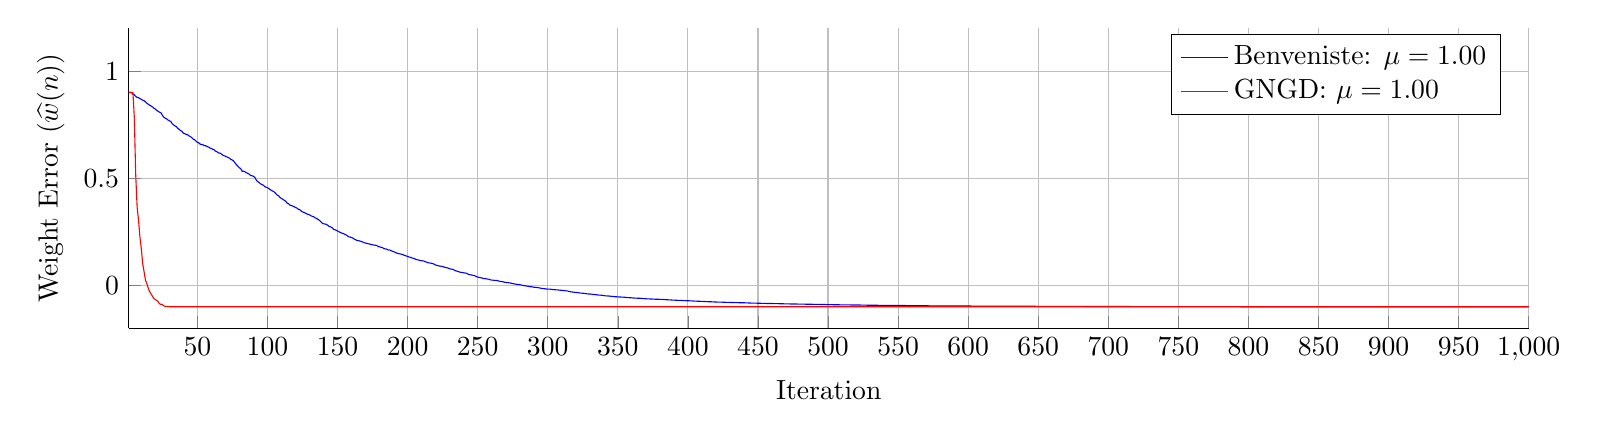
\begin{tikzpicture}

\begin{axis}[%
width=7in,
height=1.5in,
scale only axis,
xmin=1,
xmax=1000,
xlabel={Iteration},
xmajorgrids,
ymin=-0.2,
ymax=1.2,
ylabel={Weight Error ($\widehat{w}(n)$)},
ymajorgrids,
axis x line*=bottom,
axis y line*=left,
legend style={draw=black,fill=white,legend cell align=left}
]
\addplot [color=blue,solid]
  table[row sep=crcr]{1	0.9\\
2	0.9\\
3	0.9\\
4	0.89246621759067\\
5	0.889300379667029\\
6	0.882030676554208\\
7	0.877364068196871\\
8	0.875666177897206\\
9	0.871354948226354\\
10	0.867879107170633\\
11	0.864270442354246\\
12	0.861334051733481\\
13	0.855986330643285\\
14	0.849586136691085\\
15	0.845236959576214\\
16	0.840771048937967\\
17	0.836716543463529\\
18	0.832648180371729\\
19	0.82598408906249\\
20	0.823158204441232\\
21	0.817012341379359\\
22	0.81222344364225\\
23	0.808168148171388\\
24	0.805377899568316\\
25	0.793858932378786\\
26	0.785224598572891\\
27	0.780165501425037\\
28	0.777206843247355\\
29	0.771884533722887\\
30	0.768371159534594\\
31	0.764862357771896\\
32	0.754833589898165\\
33	0.748890454727399\\
34	0.743830330962112\\
35	0.740742776771595\\
36	0.732454611445811\\
37	0.728472591671019\\
38	0.722128108933738\\
39	0.719398581250228\\
40	0.710085877614675\\
41	0.707909507506167\\
42	0.704486585400023\\
43	0.703039180263328\\
44	0.6976873352632\\
45	0.693922346760395\\
46	0.689634479953993\\
47	0.682424319300464\\
48	0.679587490554477\\
49	0.672798778333772\\
50	0.667541024287875\\
51	0.665267954265584\\
52	0.658800535935858\\
53	0.657448368934852\\
54	0.655922078855278\\
55	0.652046119396351\\
56	0.651326372510181\\
57	0.647662119864227\\
58	0.64538413202839\\
59	0.640611450578998\\
60	0.638982125739482\\
61	0.634823544479989\\
62	0.632724571224535\\
63	0.626182102465582\\
64	0.623345320440783\\
65	0.618202964369375\\
66	0.617228920558395\\
67	0.613647821873813\\
68	0.608066990218837\\
69	0.60525867341197\\
70	0.60249058460536\\
71	0.599552701724071\\
72	0.596585762017137\\
73	0.59367502523378\\
74	0.586951822589198\\
75	0.585183640663902\\
76	0.579059996007459\\
77	0.570335105065955\\
78	0.562214287937066\\
79	0.555414400452733\\
80	0.548967743668685\\
81	0.543343887659217\\
82	0.532439738383363\\
83	0.532916445148112\\
84	0.529669302870372\\
85	0.525724090902359\\
86	0.522086589018822\\
87	0.519005865854083\\
88	0.513213835158974\\
89	0.511140914037441\\
90	0.509455622607838\\
91	0.503640087346894\\
92	0.492027113815121\\
93	0.4839119437404\\
94	0.480602996976824\\
95	0.474293114928524\\
96	0.470674245969945\\
97	0.467726622640063\\
98	0.461369360154249\\
99	0.45820121770722\\
100	0.455650189106997\\
101	0.452191537543344\\
102	0.446453784190006\\
103	0.442513384753563\\
104	0.438920176984734\\
105	0.43512930785166\\
106	0.427882867154837\\
107	0.421449855924578\\
108	0.418034028309152\\
109	0.409521390665955\\
110	0.405871170386572\\
111	0.401036054791144\\
112	0.396890036468093\\
113	0.392974794246107\\
114	0.38373341988298\\
115	0.381690935815512\\
116	0.374489265077057\\
117	0.372375997177259\\
118	0.370454806467114\\
119	0.366977639321656\\
120	0.363655912390095\\
121	0.360891197230356\\
122	0.355392097248246\\
123	0.353065928179253\\
124	0.347517885594097\\
125	0.34298148968504\\
126	0.340155211826512\\
127	0.337512978781199\\
128	0.334203701999589\\
129	0.330932888679365\\
130	0.329526343276441\\
131	0.324784971439447\\
132	0.322258493250213\\
133	0.320323113885022\\
134	0.314808699142924\\
135	0.312904487144416\\
136	0.30789688653086\\
137	0.304110356252179\\
138	0.297399692254421\\
139	0.290735777499623\\
140	0.287414589848527\\
141	0.286429549733006\\
142	0.284595908459977\\
143	0.280765721932813\\
144	0.274731195423071\\
145	0.272877383214771\\
146	0.269978541244004\\
147	0.262694655231315\\
148	0.259659016928578\\
149	0.257359469950497\\
150	0.253763825634715\\
151	0.250286077106786\\
152	0.246515463376409\\
153	0.243980881414783\\
154	0.24201700670436\\
155	0.238805610933443\\
156	0.235816956834633\\
157	0.231467974876412\\
158	0.22651363250011\\
159	0.225539623358514\\
160	0.22306497672838\\
161	0.220485030601734\\
162	0.215911386228065\\
163	0.212385126909046\\
164	0.209680137398688\\
165	0.20852015332244\\
166	0.206728881890613\\
167	0.204559143352569\\
168	0.202362906348626\\
169	0.198569635091692\\
170	0.197659093041998\\
171	0.19581728159039\\
172	0.193870427204048\\
173	0.192800837662292\\
174	0.19050484093328\\
175	0.189303610883971\\
176	0.188247688891546\\
177	0.187227508025501\\
178	0.186192926598871\\
179	0.18140706570032\\
180	0.179556533706728\\
181	0.177957687134788\\
182	0.175988648386967\\
183	0.172352042115338\\
184	0.170273386686173\\
185	0.169304002412893\\
186	0.165134958361591\\
187	0.165524157552452\\
188	0.162839474013205\\
189	0.159752077297533\\
190	0.157176057998391\\
191	0.154542779431521\\
192	0.151511818438805\\
193	0.148899215779492\\
194	0.147689145543227\\
195	0.146386480507473\\
196	0.144641991688906\\
197	0.14222746511545\\
198	0.139280375280982\\
199	0.137306301764167\\
200	0.134807124926226\\
201	0.132208222027054\\
202	0.131370675826319\\
203	0.128116016515823\\
204	0.126600331680684\\
205	0.124429268136671\\
206	0.120743806060263\\
207	0.119124153518939\\
208	0.118001318508404\\
209	0.115685387833808\\
210	0.115226956021181\\
211	0.114123455878656\\
212	0.112421742246564\\
213	0.109332370431863\\
214	0.107389466426266\\
215	0.105140905995781\\
216	0.104070939003629\\
217	0.103342532782739\\
218	0.101379273628979\\
219	0.0986345916676833\\
220	0.0949732350155342\\
221	0.0929872134463482\\
222	0.0910564452570711\\
223	0.0900336758049235\\
224	0.0890724401999865\\
225	0.0881541312165849\\
226	0.0853654355351614\\
227	0.0837287975476964\\
228	0.0821416905731317\\
229	0.0799778554780204\\
230	0.0778853043489115\\
231	0.0759091727572845\\
232	0.0751264057288034\\
233	0.0723068058747904\\
234	0.0685379288342208\\
235	0.0666955753087173\\
236	0.0649839728963791\\
237	0.0623603885272515\\
238	0.0607743626222135\\
239	0.0603252444113055\\
240	0.0583285342605147\\
241	0.0576826378124077\\
242	0.0567437414734672\\
243	0.0525686847880315\\
244	0.0503784955893825\\
245	0.0490668788848637\\
246	0.0477882529458873\\
247	0.0462758622057727\\
248	0.0445621107668525\\
249	0.0416935674872774\\
250	0.0387432024246703\\
251	0.0369846174634381\\
252	0.0361626607076593\\
253	0.0343128304347783\\
254	0.0320488863008518\\
255	0.0315793890598179\\
256	0.030661089718202\\
257	0.0295763852801999\\
258	0.0286742761012556\\
259	0.0260321150364312\\
260	0.0243133382690921\\
261	0.0241765403870655\\
262	0.023204194746689\\
263	0.0231226659471337\\
264	0.0226033886352924\\
265	0.0203865397794246\\
266	0.018500142286678\\
267	0.0177004499475798\\
268	0.0168184156366596\\
269	0.0149592411693614\\
270	0.0134505153764257\\
271	0.0130948581182507\\
272	0.0120427366229032\\
273	0.0115603533394689\\
274	0.00979409965605871\\
275	0.0081307914582901\\
276	0.00708018604715799\\
277	0.00567090809427795\\
278	0.0049249711899092\\
279	0.00412928252797184\\
280	0.00318457356026269\\
281	0.00181146288510858\\
282	0.00014987295530966\\
283	-0.00104295330874582\\
284	-0.00189673053437434\\
285	-0.00345069909289297\\
286	-0.00413157891849458\\
287	-0.00544194893855998\\
288	-0.00632144608920782\\
289	-0.00698295328188381\\
290	-0.00855325921725714\\
291	-0.00910736580564675\\
292	-0.00979534136781623\\
293	-0.0106522447107128\\
294	-0.0117834326568843\\
295	-0.0132230433411994\\
296	-0.0146396647910186\\
297	-0.0153538140718424\\
298	-0.0157802989181327\\
299	-0.0170097160166396\\
300	-0.0175139672183215\\
301	-0.0177903259786768\\
302	-0.0179052155410587\\
303	-0.0191484683445227\\
304	-0.0195832436492843\\
305	-0.0204176757852369\\
306	-0.0207685569432225\\
307	-0.0211305128182665\\
308	-0.0220349428453998\\
309	-0.0228114024159625\\
310	-0.0233294175154489\\
311	-0.0240707582388781\\
312	-0.0246930439588279\\
313	-0.0255385443339822\\
314	-0.0258469964612977\\
315	-0.0282626402246258\\
316	-0.0295917019978535\\
317	-0.0304833627863234\\
318	-0.0313110885452558\\
319	-0.0323310349669119\\
320	-0.0330499328174966\\
321	-0.0336871301569651\\
322	-0.0343373852290251\\
323	-0.0357822930862403\\
324	-0.0365019213264393\\
325	-0.0366085859133211\\
326	-0.0373704955119157\\
327	-0.0382530259327488\\
328	-0.0395475266305105\\
329	-0.0401328239789868\\
330	-0.0403433291842011\\
331	-0.040815524218649\\
332	-0.0419863706374635\\
333	-0.0428974623817909\\
334	-0.0434706889410483\\
335	-0.0439755616146383\\
336	-0.0450953170128799\\
337	-0.045651414874826\\
338	-0.0459301319657358\\
339	-0.0467367879272352\\
340	-0.047547825099558\\
341	-0.0487448030262209\\
342	-0.0490848910800242\\
343	-0.0496034131994906\\
344	-0.0499797165904937\\
345	-0.0508192416667864\\
346	-0.0512384454122038\\
347	-0.0523026851707025\\
348	-0.0528245913105344\\
349	-0.053238184612473\\
350	-0.0537231836508827\\
351	-0.0541243147959601\\
352	-0.054438957279662\\
353	-0.0548327936194978\\
354	-0.0551667482508424\\
355	-0.0555335117072667\\
356	-0.0562377896621614\\
357	-0.057068227616371\\
358	-0.0574526100020044\\
359	-0.0578121685369665\\
360	-0.0581521020433587\\
361	-0.0588294474248224\\
362	-0.0592594658284457\\
363	-0.0597694048422932\\
364	-0.0600037919423204\\
365	-0.0602193495214187\\
366	-0.0603491468096446\\
367	-0.061070584328745\\
368	-0.0615151913696769\\
369	-0.0619211738510163\\
370	-0.0624424729691785\\
371	-0.0629012712867022\\
372	-0.0631859009171473\\
373	-0.0634927862449267\\
374	-0.0637788224615343\\
375	-0.0639741446590999\\
376	-0.0643269072188387\\
377	-0.0647632821654204\\
378	-0.0649247907869075\\
379	-0.0649886096411222\\
380	-0.0653222553111218\\
381	-0.0654630384189394\\
382	-0.065750577071763\\
383	-0.0661013612784638\\
384	-0.0664051300192614\\
385	-0.0673059201298347\\
386	-0.0673998465594817\\
387	-0.0676326532485632\\
388	-0.0681784773646604\\
389	-0.0687458792517743\\
390	-0.069081183115961\\
391	-0.0692902413882132\\
392	-0.0695362760216778\\
393	-0.0698888380653387\\
394	-0.0701956068838127\\
395	-0.0704420556572743\\
396	-0.070781921200518\\
397	-0.0709675195641761\\
398	-0.0713758892775557\\
399	-0.071601061161502\\
400	-0.071799688854278\\
401	-0.071932820581982\\
402	-0.0723230616484717\\
403	-0.0724837399648469\\
404	-0.0731115783377685\\
405	-0.0735366860150348\\
406	-0.0738555217117326\\
407	-0.0739346362199488\\
408	-0.074243938162002\\
409	-0.0745319843394855\\
410	-0.0748739838279412\\
411	-0.0751332191174112\\
412	-0.0752731112706024\\
413	-0.0759426258334878\\
414	-0.0761211392814252\\
415	-0.076347833113482\\
416	-0.0766203021827226\\
417	-0.0767247129446937\\
418	-0.0771518229857576\\
419	-0.0774695671956799\\
420	-0.0776779759700653\\
421	-0.0779620774627288\\
422	-0.078085205046739\\
423	-0.0781501262442427\\
424	-0.0784025316995368\\
425	-0.078652519747091\\
426	-0.078790082225759\\
427	-0.0793082671767916\\
428	-0.0794666461985549\\
429	-0.0795600647418239\\
430	-0.0796996465150818\\
431	-0.0798412056782787\\
432	-0.0799986927484714\\
433	-0.0802132429335669\\
434	-0.0803891133608639\\
435	-0.0805107283107286\\
436	-0.0808834153481867\\
437	-0.0809068863475112\\
438	-0.0810469730014557\\
439	-0.0811138728793654\\
440	-0.0812196278622007\\
441	-0.0814752656114857\\
442	-0.0817602864070787\\
443	-0.0820343075424904\\
444	-0.0823431640740413\\
445	-0.082593549327117\\
446	-0.0826654111297038\\
447	-0.0828071680577122\\
448	-0.0829179737524267\\
449	-0.0831773144176964\\
450	-0.083409941125986\\
451	-0.0835117023566578\\
452	-0.0836928456459075\\
453	-0.0839010638092139\\
454	-0.0841457590261327\\
455	-0.084264806756746\\
456	-0.0844249605254612\\
457	-0.0844879508446137\\
458	-0.0845949448811868\\
459	-0.0847553817936065\\
460	-0.084779833705149\\
461	-0.0848596821022699\\
462	-0.0850425601952011\\
463	-0.0851547738916674\\
464	-0.0854648435831059\\
465	-0.0855498827389078\\
466	-0.0856253551224059\\
467	-0.0858680583980721\\
468	-0.0860248956023261\\
469	-0.0861160438975496\\
470	-0.0863020611454839\\
471	-0.0863764035622893\\
472	-0.0865163108140612\\
473	-0.0867287796749997\\
474	-0.0869032632313838\\
475	-0.0870135206195423\\
476	-0.0870846860540678\\
477	-0.0871419605901164\\
478	-0.0872073955854594\\
479	-0.0873052142453856\\
480	-0.0874090075076853\\
481	-0.0875065700929066\\
482	-0.0875973734456087\\
483	-0.0877762624690955\\
484	-0.0879371609727471\\
485	-0.0880199600692899\\
486	-0.0881083619658583\\
487	-0.0881675874981324\\
488	-0.0882811455750175\\
489	-0.0884182881344161\\
490	-0.0886007053166359\\
491	-0.0887055263189446\\
492	-0.0888101869150845\\
493	-0.0888691886114287\\
494	-0.0890824542795883\\
495	-0.0891209140858775\\
496	-0.0892301669184755\\
497	-0.0893830811630568\\
498	-0.0895245584633727\\
499	-0.089607516367873\\
500	-0.0897312436182932\\
501	-0.0899888931934317\\
502	-0.0901503272502776\\
503	-0.0901785465482515\\
504	-0.0902887487144987\\
505	-0.0904581739683843\\
506	-0.0905562890675055\\
507	-0.0906210945879975\\
508	-0.0906949173310581\\
509	-0.0908201088544564\\
510	-0.0908938663739011\\
511	-0.0909876409500725\\
512	-0.0910530793767516\\
513	-0.0911760635015338\\
514	-0.0912480211333804\\
515	-0.0913023645191782\\
516	-0.0914008500145519\\
517	-0.0914268785331472\\
518	-0.091520504062677\\
519	-0.091563108387443\\
520	-0.0916317405346305\\
521	-0.0917143494945979\\
522	-0.0917915807311439\\
523	-0.0918706622039808\\
524	-0.0919592171481254\\
525	-0.0921075991550893\\
526	-0.0923662084791675\\
527	-0.0925150956959424\\
528	-0.0925757863906008\\
529	-0.0926603079116688\\
530	-0.0927320413928795\\
531	-0.092763052483383\\
532	-0.0927889600715739\\
533	-0.0929012265266159\\
534	-0.0929656238899056\\
535	-0.0930048377852285\\
536	-0.0931077778576224\\
537	-0.0931598252841767\\
538	-0.0932357995565837\\
539	-0.0932687358282376\\
540	-0.0933188489947369\\
541	-0.0933408239157263\\
542	-0.0933907491812606\\
543	-0.0934504288594468\\
544	-0.0935331922402378\\
545	-0.0936323065439824\\
546	-0.093680409276827\\
547	-0.0937311281868168\\
548	-0.0938011440104954\\
549	-0.0938144788893412\\
550	-0.0938635272057906\\
551	-0.0939251481367842\\
552	-0.0939703327629037\\
553	-0.0940493795532571\\
554	-0.0940756233602983\\
555	-0.0941677765130136\\
556	-0.0942825523600277\\
557	-0.0943647216155329\\
558	-0.0944504846013127\\
559	-0.0945306766528577\\
560	-0.0945838137559828\\
561	-0.0946232896502603\\
562	-0.0947414118910563\\
563	-0.0948229429596628\\
564	-0.0948505770070998\\
565	-0.0948892827922784\\
566	-0.0949208075317898\\
567	-0.0949789134323676\\
568	-0.0951061597059777\\
569	-0.0952200578193511\\
570	-0.0952359041364194\\
571	-0.0953066295468646\\
572	-0.0954124936920708\\
573	-0.0954348847457591\\
574	-0.0954582299498689\\
575	-0.0955215447732671\\
576	-0.0955347773894661\\
577	-0.0956191528126992\\
578	-0.0956756318526679\\
579	-0.0957169253912479\\
580	-0.095743796584527\\
581	-0.0958186190888248\\
582	-0.0958308614020683\\
583	-0.0958458496784098\\
584	-0.0958754423171573\\
585	-0.0959076902635407\\
586	-0.0959426889941081\\
587	-0.0959636135819243\\
588	-0.0960593991783855\\
589	-0.0960592943731872\\
590	-0.0961143005100332\\
591	-0.0961339302481985\\
592	-0.0961573411768946\\
593	-0.0961750892981275\\
594	-0.0962328066260533\\
595	-0.0963420884509769\\
596	-0.0963645635953826\\
597	-0.09638820004334\\
598	-0.0964326871974569\\
599	-0.0964771170895498\\
600	-0.096504134347439\\
601	-0.0965425731618133\\
602	-0.0965546631610982\\
603	-0.0966237154020836\\
604	-0.0966589409999757\\
605	-0.0967096666705879\\
606	-0.0967586900384484\\
607	-0.0967629490984244\\
608	-0.0968024402920215\\
609	-0.0968230117445269\\
610	-0.0968555682774902\\
611	-0.0968921622701561\\
612	-0.0969098464145889\\
613	-0.0969386346017458\\
614	-0.0969559488654136\\
615	-0.0969707179387154\\
616	-0.096986288194796\\
617	-0.097005556671007\\
618	-0.0970195786617075\\
619	-0.0970678508087482\\
620	-0.0971131730136593\\
621	-0.0971670676439432\\
622	-0.0971869786540488\\
623	-0.0972019596266237\\
624	-0.0972161654026859\\
625	-0.0972665949943371\\
626	-0.0972777651961578\\
627	-0.0973239919409531\\
628	-0.0973299153543722\\
629	-0.097374260806539\\
630	-0.0974077443799103\\
631	-0.0974280717686049\\
632	-0.097441025341236\\
633	-0.0974603064615903\\
634	-0.0974784543542115\\
635	-0.0974913742594926\\
636	-0.0975047365149567\\
637	-0.0975152320719601\\
638	-0.0975310311787883\\
639	-0.0975466335432645\\
640	-0.0975619833549221\\
641	-0.0975849237049721\\
642	-0.0976017519968589\\
643	-0.097615653438088\\
644	-0.0976286340097534\\
645	-0.0976442911771258\\
646	-0.0976681358825268\\
647	-0.0976831141086105\\
648	-0.0977037872665668\\
649	-0.097764234240682\\
650	-0.0977871331102106\\
651	-0.0977979387646412\\
652	-0.0978221803448036\\
653	-0.0978360278059199\\
654	-0.0978412316841381\\
655	-0.0978661492664894\\
656	-0.0978901443692953\\
657	-0.0979356468146916\\
658	-0.0979652482844873\\
659	-0.0979815966470221\\
660	-0.0979935452879414\\
661	-0.0980101237819637\\
662	-0.0980344249577438\\
663	-0.0980527080541599\\
664	-0.0980975734506687\\
665	-0.0981122823324858\\
666	-0.0981175794391334\\
667	-0.0981511809608372\\
668	-0.0981708951932108\\
669	-0.0981787865822129\\
670	-0.0982052431739261\\
671	-0.098212554379573\\
672	-0.0982288577829037\\
673	-0.0982520629157069\\
674	-0.09826779096508\\
675	-0.098285524720013\\
676	-0.0983000449028811\\
677	-0.0983052984080585\\
678	-0.0983141864045979\\
679	-0.0983435639489799\\
680	-0.0983534263517599\\
681	-0.0983632657158185\\
682	-0.098423796540918\\
683	-0.0984628794946191\\
684	-0.0984697104947505\\
685	-0.0984814966024331\\
686	-0.0984942781956958\\
687	-0.0985103084230762\\
688	-0.098518600459209\\
689	-0.0985268000431121\\
690	-0.0985427832848002\\
691	-0.0985589633636417\\
692	-0.0985690782849797\\
693	-0.0985809393651468\\
694	-0.0985942804405484\\
695	-0.0986071708431471\\
696	-0.0986186467735909\\
697	-0.0986464219352587\\
698	-0.0986566528883221\\
699	-0.0986787303624304\\
700	-0.09870477973374\\
701	-0.0987109257377364\\
702	-0.0987194397344723\\
703	-0.098734946373597\\
704	-0.0987484086216739\\
705	-0.098763457861951\\
706	-0.0987855286881562\\
707	-0.0988016981906895\\
708	-0.0988159625623817\\
709	-0.0988350671930824\\
710	-0.0988446484922683\\
711	-0.098853532247122\\
712	-0.0988586339842241\\
713	-0.0988655271644246\\
714	-0.0988712382858142\\
715	-0.098889040785205\\
716	-0.0988911113325895\\
717	-0.0988961736352453\\
718	-0.0989102820794636\\
719	-0.0989204639077259\\
720	-0.0989336196417356\\
721	-0.0989415221581608\\
722	-0.0989531595160559\\
723	-0.0989603423696852\\
724	-0.0989643698309647\\
725	-0.0989741825538225\\
726	-0.0989873084785985\\
727	-0.0989972883430076\\
728	-0.0989999804306373\\
729	-0.099010153986388\\
730	-0.0990251373776656\\
731	-0.0990332026585136\\
732	-0.0990550890846144\\
733	-0.0990627535060039\\
734	-0.0990680830443\\
735	-0.0990761835068553\\
736	-0.0990786352251428\\
737	-0.0991040358583847\\
738	-0.0991196110898197\\
739	-0.0991178720680429\\
740	-0.0991290352344604\\
741	-0.0991393165306889\\
742	-0.0991526978014484\\
743	-0.0991657881301601\\
744	-0.099174290325759\\
745	-0.0991811487461353\\
746	-0.0992124625576398\\
747	-0.099216614113147\\
748	-0.0992244266426796\\
749	-0.0992436314784131\\
750	-0.0992557637695585\\
751	-0.0992669293289088\\
752	-0.0992709766785792\\
753	-0.099279938807407\\
754	-0.0992856900445213\\
755	-0.0992906843627382\\
756	-0.0993008686730116\\
757	-0.0993078660355913\\
758	-0.0993098508632336\\
759	-0.0993161781079275\\
760	-0.0993221758284996\\
761	-0.0993341472666145\\
762	-0.0993471244331731\\
763	-0.0993573603643171\\
764	-0.0993631316862984\\
765	-0.099369691003437\\
766	-0.0993744388259538\\
767	-0.0993786310082425\\
768	-0.0993885999573196\\
769	-0.0993979647120209\\
770	-0.099400418669006\\
771	-0.0994024345863295\\
772	-0.0994060181889562\\
773	-0.0994112540005394\\
774	-0.0994203175749406\\
775	-0.0994245466679523\\
776	-0.0994363885615035\\
777	-0.0994439260275684\\
778	-0.0994548992095996\\
779	-0.0994650039230717\\
780	-0.0994671956279173\\
781	-0.0994701961786644\\
782	-0.0994709602194455\\
783	-0.0994898055136005\\
784	-0.0994903925410805\\
785	-0.0994959828334704\\
786	-0.0995001448180416\\
787	-0.0995099030288805\\
788	-0.0995172188775033\\
789	-0.0995213916192231\\
790	-0.0995272610847798\\
791	-0.0995350262263571\\
792	-0.0995480176655553\\
793	-0.0995511576991525\\
794	-0.0995568847088341\\
795	-0.0995604671125979\\
796	-0.099566653457076\\
797	-0.0995714149857925\\
798	-0.0995732252521181\\
799	-0.0995795133138321\\
800	-0.0995900922282338\\
801	-0.0995921182631171\\
802	-0.0995936111065591\\
803	-0.0995951721745955\\
804	-0.0995983673302712\\
805	-0.0996055892744954\\
806	-0.0996129080827864\\
807	-0.099613496222438\\
808	-0.0996193089811317\\
809	-0.0996272789539159\\
810	-0.0996303348315102\\
811	-0.0996352133390758\\
812	-0.0996372778747908\\
813	-0.0996419181280099\\
814	-0.0996432293618327\\
815	-0.0996491561532037\\
816	-0.0996513081766551\\
817	-0.0996547150663725\\
818	-0.0996589065324095\\
819	-0.0996636996481391\\
820	-0.0996669352466728\\
821	-0.0996688228972126\\
822	-0.0996709432923207\\
823	-0.0996727795999114\\
824	-0.0996751202515359\\
825	-0.0996799524929421\\
826	-0.0996818199462195\\
827	-0.0996884603556168\\
828	-0.0996906665300397\\
829	-0.0996961764879047\\
830	-0.0996980145578931\\
831	-0.0997021498215244\\
832	-0.0997047070848218\\
833	-0.0997097583712756\\
834	-0.0997125571085019\\
835	-0.0997147886400613\\
836	-0.0997169349904828\\
837	-0.09972032244159\\
838	-0.0997227599801512\\
839	-0.0997237178377427\\
840	-0.0997290750275247\\
841	-0.0997332483792437\\
842	-0.0997371936969317\\
843	-0.0997378794474126\\
844	-0.0997416458349661\\
845	-0.0997447075068326\\
846	-0.0997513714391999\\
847	-0.0997577916730809\\
848	-0.0997677718839011\\
849	-0.0997683272382905\\
850	-0.0997689366473009\\
851	-0.0997701369471015\\
852	-0.0997720661873852\\
853	-0.0997744879905095\\
854	-0.0997755986554913\\
855	-0.0997795561854673\\
856	-0.0997799424062747\\
857	-0.0997839914462755\\
858	-0.0997863408453398\\
859	-0.0997886049999893\\
860	-0.0997910240014827\\
861	-0.0997931621821971\\
862	-0.0997955214906995\\
863	-0.0997969059078049\\
864	-0.0997973794659145\\
865	-0.0997985929544496\\
866	-0.0998025080897011\\
867	-0.0998072195272419\\
868	-0.0998076731878862\\
869	-0.099808866964172\\
870	-0.0998095999179938\\
871	-0.099810889172657\\
872	-0.0998133981114957\\
873	-0.0998146405989592\\
874	-0.0998165474879492\\
875	-0.0998179642201892\\
876	-0.099818878140041\\
877	-0.0998194925555991\\
878	-0.0998207766243233\\
879	-0.0998226256080951\\
880	-0.099823069359852\\
881	-0.0998245629212944\\
882	-0.0998288732531938\\
883	-0.0998308295405934\\
884	-0.0998307225070763\\
885	-0.0998328674093013\\
886	-0.0998352228007647\\
887	-0.0998362301780166\\
888	-0.0998380564484023\\
889	-0.0998410073544237\\
890	-0.0998426672559646\\
891	-0.099844140077695\\
892	-0.0998452430193147\\
893	-0.0998461422367363\\
894	-0.0998491578994162\\
895	-0.0998502666461544\\
896	-0.099852990395208\\
897	-0.0998565072662083\\
898	-0.0998583570644841\\
899	-0.099859476441763\\
900	-0.0998602925063927\\
901	-0.0998622599552949\\
902	-0.0998643125234489\\
903	-0.0998648325647824\\
904	-0.0998674686612301\\
905	-0.0998692691089559\\
906	-0.0998712465996657\\
907	-0.0998718747346956\\
908	-0.0998726930413234\\
909	-0.0998764571368671\\
910	-0.0998777383557232\\
911	-0.099879705109438\\
912	-0.09988052868897\\
913	-0.0998808632764129\\
914	-0.0998833958732867\\
915	-0.0998839088413284\\
916	-0.0998847874189728\\
917	-0.0998858405491623\\
918	-0.0998861941240535\\
919	-0.0998885650215167\\
920	-0.0998887681111993\\
921	-0.0998899821200849\\
922	-0.0998908951177215\\
923	-0.0998922042563422\\
924	-0.0998933774318341\\
925	-0.0998946842579524\\
926	-0.0998949284642945\\
927	-0.099895481409619\\
928	-0.0998961044840445\\
929	-0.0998968657086466\\
930	-0.0998986367640438\\
931	-0.0998991618149254\\
932	-0.099901101447319\\
933	-0.0999020864686564\\
934	-0.0999030073557311\\
935	-0.0999030471111225\\
936	-0.0999037091901404\\
937	-0.0999054415058662\\
938	-0.0999058522248061\\
939	-0.0999070195760424\\
940	-0.0999073530623107\\
941	-0.0999086937275923\\
942	-0.0999092257825961\\
943	-0.0999102248886464\\
944	-0.0999108414963821\\
945	-0.0999112246053896\\
946	-0.0999127152414973\\
947	-0.0999131189562753\\
948	-0.0999136509486919\\
949	-0.0999138445302007\\
950	-0.0999145673588259\\
951	-0.0999147223391771\\
952	-0.0999152597654909\\
953	-0.0999162526877342\\
954	-0.0999170848312462\\
955	-0.0999174761452512\\
956	-0.099918603506462\\
957	-0.0999187983350766\\
958	-0.099919842208224\\
959	-0.0999202593792903\\
960	-0.0999206658829594\\
961	-0.0999214855160477\\
962	-0.0999222557219633\\
963	-0.0999229875188138\\
964	-0.0999236128746533\\
965	-0.0999241913414932\\
966	-0.0999256672634186\\
967	-0.0999259065263628\\
968	-0.0999269550662009\\
969	-0.0999275566771534\\
970	-0.0999279946881035\\
971	-0.09992839381207\\
972	-0.0999291737962587\\
973	-0.0999292650493571\\
974	-0.0999293368771171\\
975	-0.0999298349282142\\
976	-0.0999306105809358\\
977	-0.099931053350506\\
978	-0.0999317599505195\\
979	-0.0999320242003057\\
980	-0.0999330451400732\\
981	-0.0999335584503477\\
982	-0.0999348401836549\\
983	-0.0999351068480756\\
984	-0.0999354601168402\\
985	-0.0999362841258969\\
986	-0.0999372986845017\\
987	-0.0999380444106348\\
988	-0.0999382651718749\\
989	-0.0999388021628421\\
990	-0.0999394972737294\\
991	-0.0999399270339506\\
992	-0.099940225827807\\
993	-0.0999414779096899\\
994	-0.0999421992912859\\
995	-0.099943823071645\\
996	-0.0999448037862857\\
997	-0.0999460917965995\\
998	-0.0999468106379876\\
999	-0.0999475218192464\\
1000	-0.0999478331987808\\
1001	-0.0999482547934084\\
};
\addlegendentry{Benveniste: $\mu=1.00$};

\addplot [color=red,solid]
  table[row sep=crcr]{1	0.9\\
2	0.9\\
3	0.9\\
4	0.9\\
5	0.783655629436531\\
6	0.515196627266386\\
7	0.365664610573291\\
8	0.304946086861636\\
9	0.225638986648079\\
10	0.170523042753516\\
11	0.100526642272392\\
12	0.0627946893961063\\
13	0.0235375399243068\\
14	0.0066595500881379\\
15	-0.0146462943183548\\
16	-0.0300306906035475\\
17	-0.0409408115977464\\
18	-0.0510190919481683\\
19	-0.0622081547064791\\
20	-0.0663619951342344\\
21	-0.0705513697850059\\
22	-0.0765955492415521\\
23	-0.0859621451971841\\
24	-0.0885118374673881\\
25	-0.0891011753393834\\
26	-0.0958104145765111\\
27	-0.0976974221343869\\
28	-0.0980481382948669\\
29	-0.0988166211218769\\
30	-0.0995502796072728\\
31	-0.0997787786459632\\
32	-0.0996020418044085\\
33	-0.0997363421951224\\
34	-0.0998941947827189\\
35	-0.0997790073013795\\
36	-0.0998505236043756\\
37	-0.0998778767918722\\
38	-0.0998823260704876\\
39	-0.0999255139859981\\
40	-0.0999740327469644\\
41	-0.0999882711002286\\
42	-0.0999796209550166\\
43	-0.0999834798166404\\
44	-0.099985346398643\\
45	-0.0999772573930325\\
46	-0.0999793545423525\\
47	-0.100002399969823\\
48	-0.0999907826171139\\
49	-0.0999923736898479\\
50	-0.0999898451567057\\
51	-0.0999904308667675\\
52	-0.099994571287656\\
53	-0.0999919013063746\\
54	-0.0999951216525893\\
55	-0.0999957035008406\\
56	-0.0999957006373483\\
57	-0.0999967557630752\\
58	-0.0999973810215202\\
59	-0.099997368321023\\
60	-0.0999991312668586\\
61	-0.0999985585938452\\
62	-0.099999252632219\\
63	-0.0999998282702075\\
64	-0.0999996755922982\\
65	-0.10000014751203\\
66	-0.100000205916566\\
67	-0.100000196401621\\
68	-0.100000228576683\\
69	-0.100000050710227\\
70	-0.100000002822508\\
71	-0.0999999882449966\\
72	-0.099999971809034\\
73	-0.0999999556781057\\
74	-0.0999999290474036\\
75	-0.0999999091114103\\
76	-0.0999999614661922\\
77	-0.0999999588933217\\
78	-0.0999999664187541\\
79	-0.0999999690990355\\
80	-0.0999999671702426\\
81	-0.0999999674783637\\
82	-0.0999999844271791\\
83	-0.0999999831385031\\
84	-0.0999999880441\\
85	-0.09999999060242\\
86	-0.0999999926363416\\
87	-0.099999992983005\\
88	-0.0999999946247341\\
89	-0.0999999946192858\\
90	-0.0999999954265982\\
91	-0.0999999965299467\\
92	-0.0999999981783567\\
93	-0.0999999982677579\\
94	-0.0999999986857967\\
95	-0.0999999993679358\\
96	-0.0999999994771631\\
97	-0.0999999996708102\\
98	-0.0999999997906311\\
99	-0.0999999998572766\\
100	-0.0999999998648505\\
101	-0.0999999998928569\\
102	-0.0999999999510148\\
103	-0.0999999999505492\\
104	-0.0999999999609741\\
105	-0.0999999999690804\\
106	-0.0999999999785174\\
107	-0.0999999999798887\\
108	-0.099999999981106\\
109	-0.0999999999864579\\
110	-0.0999999999963014\\
111	-0.0999999999983224\\
112	-0.0999999999986164\\
113	-0.0999999999992859\\
114	-0.0999999999994327\\
115	-0.0999999999995441\\
116	-0.0999999999996192\\
117	-0.0999999999995813\\
118	-0.0999999999995692\\
119	-0.0999999999996081\\
120	-0.0999999999996228\\
121	-0.0999999999996565\\
122	-0.0999999999996725\\
123	-0.0999999999997346\\
124	-0.09999999999979\\
125	-0.0999999999998283\\
126	-0.0999999999998625\\
127	-0.0999999999998786\\
128	-0.0999999999999254\\
129	-0.0999999999999248\\
130	-0.0999999999999381\\
131	-0.0999999999999783\\
132	-0.0999999999999904\\
133	-0.0999999999999904\\
134	-0.0999999999999943\\
135	-0.0999999999999971\\
136	-0.0999999999999971\\
137	-0.0999999999999984\\
138	-0.0999999999999998\\
139	-0.1\\
140	-0.1\\
141	-0.1\\
142	-0.1\\
143	-0.1\\
144	-0.1\\
145	-0.1\\
146	-0.1\\
147	-0.1\\
148	-0.1\\
149	-0.1\\
150	-0.1\\
151	-0.1\\
152	-0.1\\
153	-0.1\\
154	-0.1\\
155	-0.1\\
156	-0.1\\
157	-0.1\\
158	-0.1\\
159	-0.1\\
160	-0.1\\
161	-0.1\\
162	-0.1\\
163	-0.1\\
164	-0.1\\
165	-0.1\\
166	-0.1\\
167	-0.1\\
168	-0.1\\
169	-0.1\\
170	-0.1\\
171	-0.1\\
172	-0.1\\
173	-0.1\\
174	-0.1\\
175	-0.1\\
176	-0.1\\
177	-0.1\\
178	-0.1\\
179	-0.1\\
180	-0.1\\
181	-0.1\\
182	-0.1\\
183	-0.1\\
184	-0.1\\
185	-0.1\\
186	-0.1\\
187	-0.1\\
188	-0.1\\
189	-0.1\\
190	-0.1\\
191	-0.1\\
192	-0.1\\
193	-0.1\\
194	-0.1\\
195	-0.1\\
196	-0.1\\
197	-0.1\\
198	-0.1\\
199	-0.1\\
200	-0.1\\
201	-0.1\\
202	-0.1\\
203	-0.1\\
204	-0.1\\
205	-0.1\\
206	-0.1\\
207	-0.1\\
208	-0.1\\
209	-0.1\\
210	-0.1\\
211	-0.1\\
212	-0.1\\
213	-0.1\\
214	-0.1\\
215	-0.1\\
216	-0.1\\
217	-0.1\\
218	-0.1\\
219	-0.1\\
220	-0.1\\
221	-0.1\\
222	-0.1\\
223	-0.1\\
224	-0.1\\
225	-0.1\\
226	-0.1\\
227	-0.1\\
228	-0.1\\
229	-0.1\\
230	-0.1\\
231	-0.1\\
232	-0.1\\
233	-0.1\\
234	-0.1\\
235	-0.1\\
236	-0.1\\
237	-0.1\\
238	-0.1\\
239	-0.1\\
240	-0.1\\
241	-0.1\\
242	-0.1\\
243	-0.1\\
244	-0.1\\
245	-0.1\\
246	-0.1\\
247	-0.1\\
248	-0.1\\
249	-0.1\\
250	-0.1\\
251	-0.1\\
252	-0.1\\
253	-0.1\\
254	-0.1\\
255	-0.1\\
256	-0.1\\
257	-0.1\\
258	-0.1\\
259	-0.1\\
260	-0.1\\
261	-0.1\\
262	-0.1\\
263	-0.1\\
264	-0.1\\
265	-0.1\\
266	-0.1\\
267	-0.1\\
268	-0.1\\
269	-0.1\\
270	-0.1\\
271	-0.1\\
272	-0.1\\
273	-0.1\\
274	-0.1\\
275	-0.1\\
276	-0.1\\
277	-0.1\\
278	-0.1\\
279	-0.1\\
280	-0.1\\
281	-0.1\\
282	-0.1\\
283	-0.1\\
284	-0.1\\
285	-0.1\\
286	-0.1\\
287	-0.1\\
288	-0.1\\
289	-0.1\\
290	-0.1\\
291	-0.1\\
292	-0.1\\
293	-0.1\\
294	-0.1\\
295	-0.1\\
296	-0.1\\
297	-0.1\\
298	-0.1\\
299	-0.1\\
300	-0.1\\
301	-0.1\\
302	-0.1\\
303	-0.1\\
304	-0.1\\
305	-0.1\\
306	-0.1\\
307	-0.1\\
308	-0.1\\
309	-0.1\\
310	-0.1\\
311	-0.1\\
312	-0.1\\
313	-0.1\\
314	-0.1\\
315	-0.1\\
316	-0.1\\
317	-0.1\\
318	-0.1\\
319	-0.1\\
320	-0.1\\
321	-0.1\\
322	-0.1\\
323	-0.1\\
324	-0.1\\
325	-0.1\\
326	-0.1\\
327	-0.1\\
328	-0.1\\
329	-0.1\\
330	-0.1\\
331	-0.1\\
332	-0.1\\
333	-0.1\\
334	-0.1\\
335	-0.1\\
336	-0.1\\
337	-0.1\\
338	-0.1\\
339	-0.1\\
340	-0.1\\
341	-0.1\\
342	-0.1\\
343	-0.1\\
344	-0.1\\
345	-0.1\\
346	-0.1\\
347	-0.1\\
348	-0.1\\
349	-0.1\\
350	-0.1\\
351	-0.1\\
352	-0.1\\
353	-0.1\\
354	-0.1\\
355	-0.1\\
356	-0.1\\
357	-0.1\\
358	-0.1\\
359	-0.1\\
360	-0.1\\
361	-0.1\\
362	-0.1\\
363	-0.1\\
364	-0.1\\
365	-0.1\\
366	-0.1\\
367	-0.1\\
368	-0.1\\
369	-0.1\\
370	-0.1\\
371	-0.1\\
372	-0.1\\
373	-0.1\\
374	-0.1\\
375	-0.1\\
376	-0.1\\
377	-0.1\\
378	-0.1\\
379	-0.1\\
380	-0.1\\
381	-0.1\\
382	-0.1\\
383	-0.1\\
384	-0.1\\
385	-0.1\\
386	-0.1\\
387	-0.1\\
388	-0.1\\
389	-0.1\\
390	-0.1\\
391	-0.1\\
392	-0.1\\
393	-0.1\\
394	-0.1\\
395	-0.1\\
396	-0.1\\
397	-0.1\\
398	-0.1\\
399	-0.1\\
400	-0.1\\
401	-0.1\\
402	-0.1\\
403	-0.1\\
404	-0.1\\
405	-0.1\\
406	-0.1\\
407	-0.1\\
408	-0.1\\
409	-0.1\\
410	-0.1\\
411	-0.1\\
412	-0.1\\
413	-0.1\\
414	-0.1\\
415	-0.1\\
416	-0.1\\
417	-0.1\\
418	-0.1\\
419	-0.1\\
420	-0.1\\
421	-0.1\\
422	-0.1\\
423	-0.1\\
424	-0.1\\
425	-0.1\\
426	-0.1\\
427	-0.1\\
428	-0.1\\
429	-0.1\\
430	-0.1\\
431	-0.1\\
432	-0.1\\
433	-0.1\\
434	-0.1\\
435	-0.1\\
436	-0.1\\
437	-0.1\\
438	-0.1\\
439	-0.1\\
440	-0.1\\
441	-0.1\\
442	-0.1\\
443	-0.1\\
444	-0.1\\
445	-0.1\\
446	-0.1\\
447	-0.1\\
448	-0.1\\
449	-0.1\\
450	-0.1\\
451	-0.1\\
452	-0.1\\
453	-0.1\\
454	-0.1\\
455	-0.1\\
456	-0.1\\
457	-0.1\\
458	-0.1\\
459	-0.1\\
460	-0.1\\
461	-0.1\\
462	-0.1\\
463	-0.1\\
464	-0.1\\
465	-0.1\\
466	-0.1\\
467	-0.1\\
468	-0.1\\
469	-0.1\\
470	-0.1\\
471	-0.1\\
472	-0.1\\
473	-0.1\\
474	-0.1\\
475	-0.1\\
476	-0.1\\
477	-0.1\\
478	-0.1\\
479	-0.1\\
480	-0.1\\
481	-0.1\\
482	-0.1\\
483	-0.1\\
484	-0.1\\
485	-0.1\\
486	-0.1\\
487	-0.1\\
488	-0.1\\
489	-0.1\\
490	-0.1\\
491	-0.1\\
492	-0.1\\
493	-0.1\\
494	-0.1\\
495	-0.1\\
496	-0.1\\
497	-0.1\\
498	-0.1\\
499	-0.1\\
500	-0.1\\
501	-0.1\\
502	-0.1\\
503	-0.1\\
504	-0.1\\
505	-0.1\\
506	-0.1\\
507	-0.1\\
508	-0.1\\
509	-0.1\\
510	-0.1\\
511	-0.1\\
512	-0.1\\
513	-0.1\\
514	-0.1\\
515	-0.1\\
516	-0.1\\
517	-0.1\\
518	-0.1\\
519	-0.1\\
520	-0.1\\
521	-0.1\\
522	-0.1\\
523	-0.1\\
524	-0.1\\
525	-0.1\\
526	-0.1\\
527	-0.1\\
528	-0.1\\
529	-0.1\\
530	-0.1\\
531	-0.1\\
532	-0.1\\
533	-0.1\\
534	-0.1\\
535	-0.1\\
536	-0.1\\
537	-0.1\\
538	-0.1\\
539	-0.1\\
540	-0.1\\
541	-0.1\\
542	-0.1\\
543	-0.1\\
544	-0.1\\
545	-0.1\\
546	-0.1\\
547	-0.1\\
548	-0.1\\
549	-0.1\\
550	-0.1\\
551	-0.1\\
552	-0.1\\
553	-0.1\\
554	-0.1\\
555	-0.1\\
556	-0.1\\
557	-0.1\\
558	-0.1\\
559	-0.1\\
560	-0.1\\
561	-0.1\\
562	-0.1\\
563	-0.1\\
564	-0.1\\
565	-0.1\\
566	-0.1\\
567	-0.1\\
568	-0.1\\
569	-0.1\\
570	-0.1\\
571	-0.1\\
572	-0.1\\
573	-0.1\\
574	-0.1\\
575	-0.1\\
576	-0.1\\
577	-0.1\\
578	-0.1\\
579	-0.1\\
580	-0.1\\
581	-0.1\\
582	-0.1\\
583	-0.1\\
584	-0.1\\
585	-0.1\\
586	-0.1\\
587	-0.1\\
588	-0.1\\
589	-0.1\\
590	-0.1\\
591	-0.1\\
592	-0.1\\
593	-0.1\\
594	-0.1\\
595	-0.1\\
596	-0.1\\
597	-0.1\\
598	-0.1\\
599	-0.1\\
600	-0.1\\
601	-0.1\\
602	-0.1\\
603	-0.1\\
604	-0.1\\
605	-0.1\\
606	-0.1\\
607	-0.1\\
608	-0.1\\
609	-0.1\\
610	-0.1\\
611	-0.1\\
612	-0.1\\
613	-0.1\\
614	-0.1\\
615	-0.1\\
616	-0.1\\
617	-0.1\\
618	-0.1\\
619	-0.1\\
620	-0.1\\
621	-0.1\\
622	-0.1\\
623	-0.1\\
624	-0.1\\
625	-0.1\\
626	-0.1\\
627	-0.1\\
628	-0.1\\
629	-0.1\\
630	-0.1\\
631	-0.1\\
632	-0.1\\
633	-0.1\\
634	-0.1\\
635	-0.1\\
636	-0.1\\
637	-0.1\\
638	-0.1\\
639	-0.1\\
640	-0.1\\
641	-0.1\\
642	-0.1\\
643	-0.1\\
644	-0.1\\
645	-0.1\\
646	-0.1\\
647	-0.1\\
648	-0.1\\
649	-0.1\\
650	-0.1\\
651	-0.1\\
652	-0.1\\
653	-0.1\\
654	-0.1\\
655	-0.1\\
656	-0.1\\
657	-0.1\\
658	-0.1\\
659	-0.1\\
660	-0.1\\
661	-0.1\\
662	-0.1\\
663	-0.1\\
664	-0.1\\
665	-0.1\\
666	-0.1\\
667	-0.1\\
668	-0.1\\
669	-0.1\\
670	-0.1\\
671	-0.1\\
672	-0.1\\
673	-0.1\\
674	-0.1\\
675	-0.1\\
676	-0.1\\
677	-0.1\\
678	-0.1\\
679	-0.1\\
680	-0.1\\
681	-0.1\\
682	-0.1\\
683	-0.1\\
684	-0.1\\
685	-0.1\\
686	-0.1\\
687	-0.1\\
688	-0.1\\
689	-0.1\\
690	-0.1\\
691	-0.1\\
692	-0.1\\
693	-0.1\\
694	-0.1\\
695	-0.1\\
696	-0.1\\
697	-0.1\\
698	-0.1\\
699	-0.1\\
700	-0.1\\
701	-0.1\\
702	-0.1\\
703	-0.1\\
704	-0.1\\
705	-0.1\\
706	-0.1\\
707	-0.1\\
708	-0.1\\
709	-0.1\\
710	-0.1\\
711	-0.1\\
712	-0.1\\
713	-0.1\\
714	-0.1\\
715	-0.1\\
716	-0.1\\
717	-0.1\\
718	-0.1\\
719	-0.1\\
720	-0.1\\
721	-0.1\\
722	-0.1\\
723	-0.1\\
724	-0.1\\
725	-0.1\\
726	-0.1\\
727	-0.1\\
728	-0.1\\
729	-0.1\\
730	-0.1\\
731	-0.1\\
732	-0.1\\
733	-0.1\\
734	-0.1\\
735	-0.1\\
736	-0.1\\
737	-0.1\\
738	-0.1\\
739	-0.1\\
740	-0.1\\
741	-0.1\\
742	-0.1\\
743	-0.1\\
744	-0.1\\
745	-0.1\\
746	-0.1\\
747	-0.1\\
748	-0.1\\
749	-0.1\\
750	-0.1\\
751	-0.1\\
752	-0.1\\
753	-0.1\\
754	-0.1\\
755	-0.1\\
756	-0.1\\
757	-0.1\\
758	-0.1\\
759	-0.1\\
760	-0.1\\
761	-0.1\\
762	-0.1\\
763	-0.1\\
764	-0.1\\
765	-0.1\\
766	-0.1\\
767	-0.1\\
768	-0.1\\
769	-0.1\\
770	-0.1\\
771	-0.1\\
772	-0.1\\
773	-0.1\\
774	-0.1\\
775	-0.1\\
776	-0.1\\
777	-0.1\\
778	-0.1\\
779	-0.1\\
780	-0.1\\
781	-0.1\\
782	-0.1\\
783	-0.1\\
784	-0.1\\
785	-0.1\\
786	-0.1\\
787	-0.1\\
788	-0.1\\
789	-0.1\\
790	-0.1\\
791	-0.1\\
792	-0.1\\
793	-0.1\\
794	-0.1\\
795	-0.1\\
796	-0.1\\
797	-0.1\\
798	-0.1\\
799	-0.1\\
800	-0.1\\
801	-0.1\\
802	-0.1\\
803	-0.1\\
804	-0.1\\
805	-0.1\\
806	-0.1\\
807	-0.1\\
808	-0.1\\
809	-0.1\\
810	-0.1\\
811	-0.1\\
812	-0.1\\
813	-0.1\\
814	-0.1\\
815	-0.1\\
816	-0.1\\
817	-0.1\\
818	-0.1\\
819	-0.1\\
820	-0.1\\
821	-0.1\\
822	-0.1\\
823	-0.1\\
824	-0.1\\
825	-0.1\\
826	-0.1\\
827	-0.1\\
828	-0.1\\
829	-0.1\\
830	-0.1\\
831	-0.1\\
832	-0.1\\
833	-0.1\\
834	-0.1\\
835	-0.1\\
836	-0.1\\
837	-0.1\\
838	-0.1\\
839	-0.1\\
840	-0.1\\
841	-0.1\\
842	-0.1\\
843	-0.1\\
844	-0.1\\
845	-0.1\\
846	-0.1\\
847	-0.1\\
848	-0.1\\
849	-0.1\\
850	-0.1\\
851	-0.1\\
852	-0.1\\
853	-0.1\\
854	-0.1\\
855	-0.1\\
856	-0.1\\
857	-0.1\\
858	-0.1\\
859	-0.1\\
860	-0.1\\
861	-0.1\\
862	-0.1\\
863	-0.1\\
864	-0.1\\
865	-0.1\\
866	-0.1\\
867	-0.1\\
868	-0.1\\
869	-0.1\\
870	-0.1\\
871	-0.1\\
872	-0.1\\
873	-0.1\\
874	-0.1\\
875	-0.1\\
876	-0.1\\
877	-0.1\\
878	-0.1\\
879	-0.1\\
880	-0.1\\
881	-0.1\\
882	-0.1\\
883	-0.1\\
884	-0.1\\
885	-0.1\\
886	-0.1\\
887	-0.1\\
888	-0.1\\
889	-0.1\\
890	-0.1\\
891	-0.1\\
892	-0.1\\
893	-0.1\\
894	-0.1\\
895	-0.1\\
896	-0.1\\
897	-0.1\\
898	-0.1\\
899	-0.1\\
900	-0.1\\
901	-0.1\\
902	-0.1\\
903	-0.1\\
904	-0.1\\
905	-0.1\\
906	-0.1\\
907	-0.1\\
908	-0.1\\
909	-0.1\\
910	-0.1\\
911	-0.1\\
912	-0.1\\
913	-0.1\\
914	-0.1\\
915	-0.1\\
916	-0.1\\
917	-0.1\\
918	-0.1\\
919	-0.1\\
920	-0.1\\
921	-0.1\\
922	-0.1\\
923	-0.1\\
924	-0.1\\
925	-0.1\\
926	-0.1\\
927	-0.1\\
928	-0.1\\
929	-0.1\\
930	-0.1\\
931	-0.1\\
932	-0.1\\
933	-0.1\\
934	-0.1\\
935	-0.1\\
936	-0.1\\
937	-0.1\\
938	-0.1\\
939	-0.1\\
940	-0.1\\
941	-0.1\\
942	-0.1\\
943	-0.1\\
944	-0.1\\
945	-0.1\\
946	-0.1\\
947	-0.1\\
948	-0.1\\
949	-0.1\\
950	-0.1\\
951	-0.1\\
952	-0.1\\
953	-0.1\\
954	-0.1\\
955	-0.1\\
956	-0.1\\
957	-0.1\\
958	-0.1\\
959	-0.1\\
960	-0.1\\
961	-0.1\\
962	-0.1\\
963	-0.1\\
964	-0.1\\
965	-0.1\\
966	-0.1\\
967	-0.1\\
968	-0.1\\
969	-0.1\\
970	-0.1\\
971	-0.1\\
972	-0.1\\
973	-0.1\\
974	-0.1\\
975	-0.1\\
976	-0.1\\
977	-0.1\\
978	-0.1\\
979	-0.1\\
980	-0.1\\
981	-0.1\\
982	-0.1\\
983	-0.1\\
984	-0.1\\
985	-0.1\\
986	-0.1\\
987	-0.1\\
988	-0.1\\
989	-0.1\\
990	-0.1\\
991	-0.1\\
992	-0.1\\
993	-0.1\\
994	-0.1\\
995	-0.1\\
996	-0.1\\
997	-0.1\\
998	-0.1\\
999	-0.1\\
1000	-0.1\\
1001	-0.1\\
};
\addlegendentry{GNGD: $\mu=1.00$};

\end{axis}
\end{tikzpicture}%}
	\caption{\textit{LMS filter error (dB) for the given AR process, averaged over 100 independent trials}}
	\label{fig:3_2_c}
\end{figure}

\end{document}

